% This template was initially provided by Dulip Withanage.
% Modifications were made by Conny Junghans, Jannik Strötgen, and Sascha Hunold

\documentclass[
     12pt,
     a4paper,
     BCOR=10mm,
     DIV=14,
     listof=totoc,
     bibliography=totoc,
     parskip,
     twoside,
     headsepline
     ]{scrreprt}

%%%%%%%%%%%%%%%%%%%%%%%%%%%%%%%%%%%%%%%%%%%%%%%%%%%%%%%%%%%%%%%%%%%%%%%%%%%%%%%%

% PACKAGES:

\usepackage[english]{babel}
\usepackage[utf8]{inputenc}
\usepackage{lmodern}
\usepackage[T1]{fontenc}

\makeatletter

\newcommand*\lmtt@fillM[1]{%
  \DeclareFontShape{T1}{lmtt}{#1}{n}{<->ssub*lmtt/m/n}{}%
  \DeclareFontShape{T1}{lmtt}{#1}{it}{<->ssub*lmtt/m/it}{}%
  \DeclareFontShape{T1}{lmtt}{#1}{sl}{<->ssub*lmtt/m/sl}{}%
  \DeclareFontShape{T1}{lmtt}{#1}{sc}{<->ssub*lmtt/m/sc}{}%
  \DeclareFontShape{T1}{lmtt}{#1}{scsl}{<->ssub*lmtt/m/sl}{}%
  \DeclareFontShape{T1}{lmtt}{#1}{scit}{<->ssub*lmtt/m/it}{}%
  \DeclareFontShape{T1}{lmtt}{#1}{ui}{<->ssub*lmtt/m/n}{}%
  \DeclareFontShape{T1}{lmtt}{#1}{In}{<->ssub*lmtt/m/it}{}}

\newcommand*\lmtt@fillBold[2]{%
  \DeclareFontShape{T1}{lmtt}{#1}{n}{<->ssub*lmtt/#2/n}{}%
  \DeclareFontShape{T1}{lmtt}{#1}{it}{<->ssub*lmtt/#2/sl}{}%
  \DeclareFontShape{T1}{lmtt}{#1}{sl}{<->ssub*lmtt/#2/sl}{}%
  \DeclareFontShape{T1}{lmtt}{#1}{sc}{<->ssub*lmtt/#2/n}{}%
  \DeclareFontShape{T1}{lmtt}{#1}{scsl}{<->ssub*lmtt/#2/sl}{}%
  \DeclareFontShape{T1}{lmtt}{#1}{scit}{<->ssub*lmtt/#2/sl}{}%
  \DeclareFontShape{T1}{lmtt}{#1}{ui}{<->ssub*lmtt/#2/n}{}%
  \DeclareFontShape{T1}{lmtt}{#1}{In}{<->ssub*lmtt/#2/sl}{}}

\newcommand*\lmtt@fillVariants[1]{%
  \DeclareFontShape{T1}{lmtt}{#1}{it}{<->ssub*lmtt/#1/sl}{}%
  \DeclareFontShape{T1}{lmtt}{#1}{sc}{<->ssub*lmtt/#1/n}{}%
  \DeclareFontShape{T1}{lmtt}{#1}{scsl}{<->ssub*lmtt/#1/sl}{}%
  \DeclareFontShape{T1}{lmtt}{#1}{scit}{<->ssub*lmtt/#1/sl}{}%
  \DeclareFontShape{T1}{lmtt}{#1}{ui}{<->ssub*lmtt/#1/n}{}%
  \DeclareFontShape{T1}{lmtt}{#1}{In}{<->ssub*lmtt/#1/sl}{}}

\begingroup\usefont{T1}{lmtt}{m}{n}\endgroup
\lmtt@fillVariants{b}
\lmtt@fillVariants{bx}
\DeclareFontShape{T1}{lmtt}{m}{ui}{<->ssub*lmtt/m/n}{}
\DeclareFontShape{T1}{lmtt}{m}{In}{<->ssub*lmtt/m/it}{}
\lmtt@fillM{c}
\lmtt@fillM{lc}
\lmtt@fillBold{sbx}{bx}
\lmtt@fillBold{sbc}{bx}
\lmtt@fillBold{bc}{b}
\makeatother
% Include Graphic-files:
\usepackage{graphicx}
% For math stuff
\usepackage{amsmath}
\usepackage{listings}
\usepackage{xcolor}
\usepackage{makecell}
\usepackage{multirow}
\usepackage{booktabs}
\usepackage{array}
\usepackage{tabularx}
\usepackage{ltablex}
\keepXColumns % tables opt in to page-breaking with \convertXColumns
\usepackage{geometry}
\geometry{a4paper, margin=1in}

\makeatletter
\let\hyphenat@svwarn\PackageWarning
\let\hyphenat@svwarnnl\PackageWarningNoLine
\renewcommand\PackageWarning[2]{}
\renewcommand\PackageWarningNoLine[2]{}
\usepackage[htt]{hyphenat}
\let\PackageWarning\hyphenat@svwarn
\let\PackageWarningNoLine\hyphenat@svwarnnl
\makeatother

\lstset{
    basicstyle=\footnotesize\ttfamily,
    lineskip=-1pt,                 % tighter line spacing
    breaklines=true,               % Wraps long lines
    frame=single,                  % Adds a box around the prompt
    columns=flexible,              % better space usage
    backgroundcolor=\color{gray!5},% Slight gray background
    captionpos=b                   % Puts caption at the bottom
}

% Make glossary
\usepackage[acronym, nonumberlist, toc]{glossaries}

\makenoidxglossaries
\newacronym{eai}{EAI}{Embodied Artificial Intelligence}
\newacronym{llm}{LLM}{Large Language Model}
\newacronym{ros}{ROS}{Robot Operating System 2 Humble}
\newacronym{fm}{FM}{Foundation Model}
\newacronym{yolo}{YOLO}{You Only Look Once}
\newacronym{vlm}{VLM}{Vision-Language Model}
\newacronym{rag}{RAG}{Retrieval-Augmented Generation}
\newacronym{kg}{KG}{Knowledge Graph}
\newacronym{s2r}{Sim2Real}{Simulation-to-Real}
\newacronym{vgn}{VGN}{Volumetric Grasping Network}
\newacronym{hrc}{HRC}{Human-Robot Collaboration}
\newacronym{rl}{RL}{Reinforcement Learning}
\newacronym{vla}{VLA}{Vision-Language-Action}
\newacronym{tsdf}{TSDF}{Truncated Signed Distance Function}
\newacronym{ik}{IK}{Inverse Kinematics}
\newacronym{magi}{Magistral 24B}{Magistral Small 2509 24B 4-bit Quant}
\newacronym{mini}{Ministral 14B}{Ministral 3 14B Reasoning 4-bit Quant}
\newacronym{gema44}{Gemma 4B}{Gemma 4 E4B 4-bit Quant}
\newacronym{gema42}{Gemma 2B}{Gemma 4 E2B 4-bit Quant}
\newacronym{qwen330}{Qwen 30B}{Qwen 3 VL 30B 4-bit Quant}
\newacronym{qwen38}{Qwen 8B}{Qwen 3 VL 8B 4-bit Quant}
\newacronym{cap}{CaP}{Code as Policies}
\newacronym{sgbm}{SGBM}{Semi-Global Block Matching}
\newacronym{pd}{PD}{Proportional-Derivative}
\newacronym{ompl}{OMPL}{Open Motion Planning Library}
\newacronym{urdf}{URDF}{Unified Robot Description Format}
\newacronym{cv}{CV}{Coefficient of Variation}
\newacronym{sd}{SD}{Sample Standard Deviation}
\newacronym{tfidf}{TF-IDF}{Term Frequency-Inverse Document Frequency}

\usepackage{setspace}

% hyperrefs in the documents
\usepackage[bookmarks=true,colorlinks,pdfpagelabels,pdfstartview = FitH,bookmarksopen = true,bookmarksnumbered = true,linkcolor = black,plainpages = false,hypertexnames = false,citecolor = black,urlcolor=black]{hyperref}
\usepackage{bookmark}

%%%%%%%%%%%%%%%%%%%%%%%%%%%%%%%%%%%%%%%%%%%%%%%%%%%%%%%%%%%%%%%%%%%%%%%%%%%%%%%%

% OTHER SETTINGS:

% --- Layout Fixes ---
\raggedbottom
\setlength{\emergencystretch}{3em}

\DeclareTOCStyleEntry[numwidth=2.8em]{tocline}{section}
\DeclareTOCStyleEntry[numwidth=2.8em]{tocline}{table}
\DeclareTOCStyleEntry[numwidth=2.8em]{tocline}{figure}

% Pagestyle:
\pagestyle{headings}

% Choose language
\newcommand{\setlang}[1]{\selectlanguage{#1}\nonfrenchspacing}

\begin{document}

% TITLE:
\pagenumbering{roman}
\begin{titlepage}

	\vspace*{1cm}
	\begin{center}
		\vspace*{1cm}
		\textbf{
			\Large Ruprecht Karls University of Heidelberg\\
			\smallskip
			\Large Institute for Computer Science\\
			\smallskip
			\Large Artificial Intelligence for Programming\\
			\smallskip
		}

		\vspace{3cm}

		\textbf{\large Master's Thesis}

		\vspace{2\baselineskip}
		{\huge
			Building Cooperative Robot Behavior from Basic Action Modules
		}
	\end{center}

	\vfill

	{\large
		\begin{tabular}[l]{ll}
			Name:                 & Jan Michael Straub        \\
			Matriculation Number: & 34 05 670                 \\
			Supervisor:           & Prof. Dr. Artur Andrzejak \\
			Date of Submission:   & 15.07.2026
		\end{tabular}
	}

\end{titlepage}

\onehalfspacing

\thispagestyle{empty}

\vspace*{30pt}

\section*{Declaration of Authorship and AI Usage}

I hereby declare that I have written this Master's thesis independently and have used no other sources or aids than those specified. Furthermore, regarding the use of Artificial Intelligence (AI) tools in this work, I declare that:

\begin{itemize}
	\item I assume full responsibility for the scholarly quality and content of the submitted work, the chosen methodology, the production process, and the cited literature.
	\item I confirm that the work was prepared in compliance with the principles of good academic practice (see guidelines on good academic practice).
	\item I confirm that the use of AI tools was agreed in advance with the instructor or examiner and that the agreed rules were followed.
\end{itemize}

\vspace{1.5em}

\begin{flushright}
	\begin{minipage}{20em}
		\rule{\textwidth}{0.5pt}\\
		Jan M. Straub \\
		Heidelberg, \today
	\end{minipage}
\end{flushright}

\clearpage

\vspace*{30pt}

\subsection*{Overview of AI Tools Used}

\begin{tabularx}{\textwidth}{>{\raggedright\arraybackslash}X >{\raggedright\arraybackslash}X >{\raggedright\arraybackslash}X}
	\toprule
	\textbf{AI Tool}          & \textbf{Purpose of Use}                                  & \textbf{Comments}                                                    \\
	\midrule
	Claude                    & Drafting, language editing and proofreading              & Everything was reviewed by me                                        \\
	Claude Code               & Implementation, error/bug fixing, and prompt engineering & Used as an assistant, and all code was reviewed, tested, and revised \\
	Ministral-3 14B Reasoning & Planning model                                           & Used for tests and benchmarks                                        \\
	Magistral Small 2509      & Planning model                                           & Default model used for tests, benchmarks, and system operation       \\
	Qwen3-VL 8B / 30B         & Planning model                                           & Used for tests and benchmarks                                        \\
	Gemma-4 E2B / E4B         & Planning model                                           & Used for tests and benchmarks                                        \\
	\bottomrule
\end{tabularx}

\cleardoublepage

\section*{Abstract}
Current robotic systems excel at precision in rigid sequences, yet frequently fail in unknown situations. Large Language Models (LLMs) promise to close this gap through their reasoning capabilities, even though they currently cannot turn that reasoning into physical action on their own. In this work, we present an LLM-driven control framework for two AR4 robotic arms that enables precisely this transition. To achieve this, we equip a locally hosted Vision-Language Model (VLM) with a pool of 20 operations, which the model assembles into executable chains. A Retrieval-Augmented Generation (RAG)-assisted pipeline processes natural-language instructions, a reflection mechanism retries faulty sequences, and an optional multi-agent negotiation protocol coordinates multiple robots. We implement the system in Unity using Robot Operating System (ROS) 2 and MoveIt as the collision-aware planning backend, and evaluate it across 17 benchmarks. With Magistral Small 2509 24B 4-bit Quant as the default backend model, it achieves a success rate of 1.000 across all five single-robot benchmarks and object handovers between the two arms. Additionally, ablation studies demonstrate that, with the default model, enabling the Volumetric Grasping Network (VGN) grasp path improves grasp reliability by 35 percentage points, negotiation improves task success by 10 percentage points, and the reflection mechanism improves task success by 14 percentage points. However, simultaneous manipulation of a single object remains unsolved.

\clearpage

\section*{Zusammenfassung}
Heutige Robotersysteme glänzen durch Präzision in starren Abläufen, scheitern jedoch oft noch an unvorhergesehenen Situationen. Große Sprachmodelle (LLMs) versprechen, diese Lücke durch ihre Schlussfolgerungsfähigkeit zu schließen, auch wenn ihnen bislang die Fähigkeit fehlt, abstraktes Schlussfolgern in physisches Handeln umzusetzen. In dieser Arbeit stellen wir ein LLM-gesteuertes Kontrollframework für zwei AR4-Roboterarme vor, das genau diesen Übergang ermöglicht. Wir statten dafür ein lokal betriebenes Vision-Language-Modell (VLM) mit einem Pool aus 20 Operationen aus und lassen es aus sprachlichen Anweisungen selbstständig ausführbare Operationsketten zusammensetzen. Eine Retrieval-Augmented-Generation (RAG)-gestützte Pipeline begrenzt die Anzahl möglicher Operationen. Ein Reflexionsmechanismus korrigiert fehlerhafte Schritte, und ein optionales Multi-Agenten-Verhandlungsprotokoll koordiniert mehrere Roboter. Wir implementieren das System in einer Unity-Simulation mit Robot Operating System (ROS) 2 und MoveIt als kollisionsbewusstem Planungs-Backend und evaluieren es anhand von 17 Benchmarks. Mit dem Magistral Small 2509 24B 4-bit Quant als Standard-Backend-Modell erreicht es einen 100\%igen Erfolg bei allen fünf Einzelrobotertests sowie bei der Objektübergabe zwischen beiden Robotern. Ablationsstudien zeigen zudem, dass die Aktivierung des Volumetric-Grasping-Network-(VGN)-Greifpfads die Greifzuverlässigkeit um 35 Prozentpunkte, das Verhandlungsprotokoll den Aufgabenerfolg um 10 Prozentpunkte und die Reflexion um 14 Prozentpunkte erhöht. Die gleichzeitige Manipulation eines Objekts bleibt jedoch ungelöst.

\cleardoublepage

\tableofcontents
\clearpage

\printnoidxglossary[
	type=\acronymtype,
	title=List of Abbreviations,
	nonumberlist,
	style=listdotted,
	nogroupskip,
]

\cleardoublepage

\pagenumbering{arabic}

\cleardoublepage

\glsresetall

%%%%%%%%%%%%%%%%%%%%%%%%%%%%%%%%%%%%%%%%%%%%%%%%%%%%%%%%%%%%%%%%%%%%%%%%%%%%%%%%
%%  INTRODUCTION
%%%%%%%%%%%%%%%%%%%%%%%%%%%%%%%%%%%%%%%%%%%%%%%%%%%%%%%%%%%%%%%%%%%%%%%%%%%%%%%%
\chapter{Introduction}\label{intro}
Since the introduction of Unimate in the early 1960s, robotic systems have been central to industrial manufacturing. In the automotive sector in particular, specialized robotic arms execute repetitive tasks such as painting, welding, and assembly with accuracy and speed. These operations, however, required a deterministic environment, so robots were confined to cages and pre-programmed paths, since any unplanned event could cause errors or safety hazards. Sensors and adaptive control changed this, enabling robots to absorb minor environmental variation \cite{Li2020}. The arrival of language models has pushed this further, as robots are beginning to navigate unfamiliar conditions with minimal human control, drawing on the world knowledge and reasoning these models provide.

This progress has enabled the field of \gls{eai}, where a model is embedded in a robotic body to close the loop between perception and action \cite{liu2025aligningcyberspacephysical}. Yet planning a task is not the same as executing it, and a gap remains between a model’s reasoning and a robot’s physical movement. Precise coordination is still difficult, and many models struggle with temporal consistency, failing to account for past physical states when planning future movements.

In this thesis, we bridge that disconnect with a framework that merges \gls{ros}~\cite{Macenski_2022} and MoveIt~\cite{coleman2014reducingbarrierentrycomplex} for motion planning, together with a \gls{yolo}-based~\cite{yolov8_ultralytics} vision pipeline for environmental awareness. To handle reasoning, we augment a \gls{vlm}~\cite{mistral_magistral_small_2025} with \gls{rag}~\cite{lewis2021retrievalaugmentedgenerationknowledgeintensivenlp} and an optional \gls{kg}~\cite{Hogan_2021}. Together, the stack can translate natural-language instructions into concrete, executable robot commands. Our novel contribution is an integrated architecture that combines planning, perception, and reasoning for coordinated robot control. The architecture aims at eventual \gls{s2r} deployment, but we build and validate it inside a Unity~\cite{unity} simulation. Ultimately, we aim to show that \glspl{vlm} can coordinate genuine, autonomous action between two robotic arms working toward a shared goal.

The rest of this chapter covers our motivation, objectives, and contributions. Chapter~\ref{background} summarizes related work, from early semantic planning to modern deployment frameworks. Chapter~\ref{methodology} lays out the system design and the reasoning behind it, from the operation system and the \gls{vlm}-driven command pipeline through to multi-robot coordination. Chapter~\ref{implementation} covers the implementation and the engineering decisions that mattered most. In Chapter~\ref{evaluation}, we define our benchmarks, present the results, and report an ablation for each component. Chapter~\ref{discussion} discusses the limitations of our evaluation and the open questions it leaves. Chapter~\ref{conclusion} closes with our contributions and future directions.

% ------------------------------------------------------------------------------
\section{Motivation}
Most \gls{eai} research focuses on single-agent tasks, yet many of the applications with the highest automation value are cooperative. Moving from a single arm to two introduces a new class of problems a lone robot never faces, because the arms must avoid colliding not only with objects but also with each other, and must synchronize their timing. Even with the rapid progress of language models, translating digital reasoning into reliable physical execution remains a challenge.

General-purpose models are also prone to hallucinating actions and lack the operational memory required by multi-stage task chains. To address this, we ground the model’s reasoning in live perception. A \gls{rag} operation pool restricts it to a vocabulary of executable actions, and a vision system resolves manipulation targets from current stereo detections, keeping its picture of the scene up to date.

This motivates a pipeline in which the reasoning model works as a high-level coordinator, selecting and ordering operations from a shared pool at runtime and translating intent into executable trajectories through \gls{ros} and MoveIt. Building this in a Unity-based simulation also creates a safe, scalable environment to develop these behaviors before they ever touch a physical motor.

% ------------------------------------------------------------------------------
\section{Goals, Novelty and Contributions}\label{sec:goals}\label{sec:novelty}
We set out to build an autonomous robotic operation framework driven by a reasoning \gls{vlm}, validated in simulation, and designed for physical deployment. The system accepts natural-language instructions and generates coordinated behavior without fine-tuning, hard-coded sequencing, or cloud-service dependencies. We build it in a Unity simulation with two AR4~\cite{AnninRobotics2026} arms, each behind a hardware abstraction layer.

The novelty is not a new model or control algorithm, as every component is based on previous work. The contribution is a runtime composition of behavior between two arms by a model that reasons over a shared vocabulary of basic operations, rather than a fixed execution path. The model selects, orders, and parameterizes the coordination primitives itself. The retrieval layer and the prompt supply handoff and synchronization priors, and the model applies them more reliably than it would if it had to rediscover them on its own (Section~\ref{sec:results-dual}). Prior systems side-step even that, assigning independent robots~\cite{ahn2024autortembodiedfoundationmodels} or negotiating through open dialogue~\cite{mandi2023rocodialecticmultirobotcollaboration}. Runtime composition of shared-object coordination from a fixed set of operations remains unexplored.

Five contributions build out this claim. First, a retrieval-grounded pipeline, built on a hierarchical registry of 20 operations, separates reasoning from execution. It combines \gls{rag} retrieval, a two-phase chain-of-thought decomposition inspired by RT-H~\cite{belkhale2024rthactionhierarchiesusing}, and a variable-passing mechanism that threads perception outputs into later operation parameters at runtime. Second, the coordination behind that claim runs on general-purpose primitives. The \gls{vlm} assembles signal/wait and parallel-group operations into time-ordered handoffs, parallel scheduling, and re-detection. The prompt supplies the handoff and synchronization rules, while the model chooses which primitives to use and how to combine them. Third, a consensus-gated negotiation protocol, inspired by RoCo~\cite{mandi2023rocodialecticmultirobotcollaboration} but without its free-form dialectic. Each robot gets its own agent, and the protocol runs a three-phase analysis–proposal–evaluation cycle. One agent drafts a complete plan per round in round-robin order; every peer must accept it, and the system falls back to single-model parsing if no consensus is reached within three rounds. Its B13 ablation shows a measurable but model-specific effect. For the default backend, per-task success rises $+10$~percentage points (pp), though the benefit does not generalize across models. Fourth, an operation-gated reflection mechanism re-queries the parser with an operation’s own recovery suggestions, for eligible operation categories only, clearing transient failures that a naive retry fixes (B12, $+14$~pp at the task level, $+7.0$~pp at the per-operation level). Fifth, an AutoRT adaptation for fixed-base manipulation swaps the raw-image scene representation for a structured object manifest and extends the prompt-encoded Robot Constitution with a hard kinematic layer (workspace bounds, velocity, gripper force, and minimum robot separation) that the semantic filter cannot override. Throughout, we isolate each component using single-flag ablations rather than reporting only aggregate success.

% ------------------------------------------------------------------------------
\section{Extensibility and Reusability}\label{sec:extensibility}
Because this system is intended to outlive the present thesis and serve as a foundation for later student projects, several engineering choices are designed to keep it extensible. The Python backend is split into strict dependency layers with centralized lazy imports, which avoids the circular-import failures that a growing research codebase accumulates and makes clear where new code belongs. New robot behavior has a single extension point. A contributor writes one \texttt{BasicOperation} with its parameter schema and optional metadata, registers it, and it propagates automatically to every subsystem that reads the registry as its single source of truth (Appendix~\ref{appendix:operation_example}). Camera and hardware interfaces sit behind adapters that isolate the rest of the system from the simulation/hardware distinction, so a move to physical hardware is localized to those adapters (Section~\ref{sec:sim-to-real}); tunable values live in dedicated configuration modules and Unity ScriptableObject \texttt{.asset} files (Appendix~\ref{appendix:config}); and each major subsystem is independently toggleable through its own feature flag. A regression test suite guards both halves of the system, with Python tests covering the operation registry, orchestrators, protocol handling, and the integration paths, while a Unity C\# test suite exercises the \gls{ik} solver, grasp pipeline, robot and trajectory controllers, and the wire protocol. Together, they give future contributors a safety net that catches breakage when they extend or refactor the system. The system also degrades gracefully when a piece is missing. Retrieval falls back to \gls{tfidf}, parsing to a regex matcher, negotiation to single-model parsing, and \gls{ros}/MoveIt motion to the built-in Unity controller, so the rest keeps running while one component is under development.
%%%%%%%%%%%%%%%%%%%%%%%%%%%%%%%%%%%%%%%%%%%%%%%%%%%%%%%%%%%%%%%%%%%%%%%%%%%%%%%%
%%  BACKGROUND AND RELATED WORK
%%%%%%%%%%%%%%%%%%%%%%%%%%%%%%%%%%%%%%%%%%%%%%%%%%%%%%%%%%%%%%%%%%%%%%%%%%%%%%%%
\chapter{Background and Related Work}\label{background}
The history of robotics traces a gradual shift from rigid, pre-scripted automation toward systems capable of flexible interaction with unstructured settings and human collaborators. As Li \emph{et al.}~\cite{Li2020} note, traditional manufacturing robots were high-precision, deterministic tools within strict safety zones, where human-robot interaction was kept to a minimum to avoid injury. In these environments, robots executed pre-programmed trajectories with little to no capacity for environmental sensing or real-time adjustment. This baseline lays the groundwork for the subsequent move toward interactive systems.

\gls{hrc} research sought to overcome these constraints and enable robots to work alongside humans. Even so, early systems struggled with the semantic gap, the fundamental difficulty of translating high-level human intent into low-level motor commands that a robot can reliably execute.

The response to this gap was \gls{eai}, which grounds intelligence in a physical embodiment and requires constant interaction with the environment \cite{Li2026}. In this view, an embodied agent must perceive, act upon, and learn from the physical world rather than reason over abstract symbols alone.

But learning from the physical world at scale is exactly where this ambition meets a hard constraint, as diverse, real-world interaction data is slow and costly to collect. This bottleneck spurred the development of large-scale procedural generation frameworks such as ProcTHOR~\cite{deitke2022procthorlargescaleembodiedai}. These systems train agents across thousands of auto-generated indoor environments. More recent work, such as the Unity Reinforcement Learning Playground~\cite{ye2025unityrlplaygroundversatile}, further refines simulation-based training by introducing versatile \gls{rl} frameworks for mobile robots and explicit \gls{s2r} support. Together, these approaches treat simulation not as a simplified proxy but as a structured pipeline toward real deployment.

The use of \glspl{fm}, which extend language models to encompass diverse sensory modalities such as vision and audio, has proven essential for the current generation of \gls{hrc} systems. Building on this integration, the remainder of this chapter traces the field's main phases, from semantic reasoning and grasp planning to end-to-end paradigms, edge deployment limits, skill-library composition, structured execution, hierarchical safety, fleet-scale management, and multi-robot coordination.

% ------------------------------------------------------------------------------
\section{Semantic Reasoning and Task Planning}
Early demonstrations such as ChatGPT for Robotics by Vemprala \emph{et al.}~\cite{vemprala2023chatgptroboticsdesignprinciples} and Voyager by Wang \emph{et al.}~\cite{wang2023voyageropenendedembodiedagent} established that \glspl{llm} could serve as high-level task planners, generating code sequences or natural language plans to split complex tasks. These works revealed the potential of language as an interface between human intent and robotic execution. At the same time, they exposed the limitations of text-only reasoning in physically grounded settings.

Liang \emph{et al.}~\cite{liang2023codepolicieslanguagemodel} addressed the translation of plans into executable policies in \gls{cap}, demonstrating that code-writing \glspl{llm} can translate natural language commands into robot policy code that chains perception APIs with control primitives. Unlike plan-based approaches that assume a fixed skill library, \gls{cap} writes parameterized control logic on the fly, thereby generalizing to unseen instructions without task-specific training. The key insight is that representing code as policies rather than as sequences of predefined skills enables the system to compose novel behaviors at runtime, advancing planning into execution.

Where \gls{cap} operates at the level of individual workspaces, Rana \emph{et al.}~\cite{rana2023sayplangroundinglargelanguage} tackled the challenge of scaling language-based planning to large, multi-room environments with SayPlan. By grounding an \gls{llm} in 3D scene graphs, SayPlan enables task planning within environments that are far too large for a single model to process in its entirety. Semantic search over a collapsed scene-graph representation expands only the task-relevant subgraph, keeping the model’s context window manageable while preserving awareness of the global structure; a separate iterative replanning loop then validates each draft plan against a scene-graph simulator and feeds infeasible actions back for correction. This is relevant for multi-robot coordination, where agents must reason about objects and workspaces beyond their immediate field of view, extending the same planning logic to larger settings.

% ------------------------------------------------------------------------------
\section{Grasp Planning and Physical Grounding}
While semantic planners provide the strategic plan for complex tasks, effective execution relies on the robot’s ability to physically engage with discrete objects. High-level planners, therefore, define what must be done, whereas grasp planning determines the specific mechanics of physically engaging the environment. As the survey by Newbury \emph{et al.}~\cite{newbury2023deeplearningapproachesgrasp} points out, the field has moved from analytic force-closure methods toward data-driven approaches that learn grasp quality directly from sensor observations. Large-scale benchmarks such as GraspNet-1Billion~\cite{graspnet} and frameworks such as Contact-GraspNet~\cite{sundermeyer2021contactgraspnetefficient6dofgrasp} and AnyGrasp~\cite{fang2023anygrasprobustefficientgrasp} drove this shift, with the latter supporting real-time 7-DOF candidate generation for unseen objects in cluttered scenes.

Given this system’s infrastructure-independent deployment goals, inference speed and deployment simplicity are decisive considerations. \gls{vgn}~\cite{breyer2021volumetricgraspingnetworkrealtime} addresses these constraints by representing the scene as a \gls{tsdf} voxel grid. Using this grid, it predicts grasp quality, orientation, and gripper width in a single forward pass, reducing planning time to approximately 10 ms. This approach also provides implicit collision awareness and zero-shot transfer from simulation to real hardware.

% ------------------------------------------------------------------------------
\section{End-to-End Control}
Building on this progression, the field subsequently shifted toward \gls{vla} models, in which a single architecture consumes visual and linguistic inputs to directly produce motor commands. PaLM-E~\cite{driess2023palmeembodiedmultimodallanguage} injects images, state estimates, and other modalities directly into the embedding space of a pre-trained language model, enabling grounded, multi-embodiment robotic planning. A single model, scaled up to 562 billion parameters, was trained across multiple robotic manipulation domains, demonstrating positive transfer across the visual-language and embodied reasoning domains.

Extending this line of work, RT-2~\cite{brohan2023rt2visionlanguageactionmodelstransfer} showed that \gls{vla} models trained on internet-scale vision-language data can transfer broad semantic knowledge, including logical reasoning and common-sense understanding, to robot manipulation tasks. This enabled generalization to object categories and scenarios completely absent from the robot’s physical training data.

% ------------------------------------------------------------------------------
\section{Computing Constraints and Edge Deployment}
A major challenge in moving \gls{eai} beyond the laboratory is the tension between model scale and the latency constraints of physical systems. End-to-end models such as RT-2~\cite{brohan2023rt2visionlanguageactionmodelstransfer} and PaLM-E~\cite{driess2023palmeembodiedmultimodallanguage} achieve impressive semantic generalization, but their parameter counts require computational infrastructure incompatible with mobile or resource-limited platforms.

As Grover \emph{et al.}~\cite{grover2026embodiedfoundationmodelsedge} and Kim \emph{et al.}~\cite{kim2024openvlaopensourcevisionlanguageactionmodel} note, running a large \gls{vla} is slow in two ways. Interpreting camera and language input is computationally expensive, and producing each action one step at a time is constrained by memory speed. Together, these constraints keep most models to fewer than five updates per second. That is too slow for close collaboration.

Even edge-optimized models such as TinyVLA~\cite{wen2025tinyvlafastdataefficientvisionlanguageaction} face a persistent trade-off between reasoning accuracy and real-time reaction. This infrastructure bottleneck motivates the modular approach we take. By separating visual comprehension from physical execution, our system keeps control frequencies predictable and uses the model for semantic guidance only when a new task requires planning.

% ------------------------------------------------------------------------------
\section{Skill Libraries and Retrieval-Augmented Control}
As the computational and data demands of end-to-end \gls{vla} models became apparent, a parallel approach emerged. Rather than generating low-level control directly, \glspl{llm} are used to sequence predefined, physically verified skills from libraries. This concept adapts \gls{rag}~\cite{lewis2021retrievalaugmentedgenerationknowledgeintensivenlp} from natural language processing to the physical domain; instead of retrieving text documents to ground a model’s answers, the system retrieves parameterized control primitives or executable code blocks.

Early implementations relied on affordance models to constrain skill selection. SayCan~\cite{ahn2022icanisay} showed that a \gls{llm} can decompose high-level instructions into skill sequences, utilizing a pre-trained affordance function to evaluate whether each skill was physically feasible in the current state. Voyager~\cite{wang2023voyageropenendedembodiedagent} extended this concept, demonstrating that agents could not only retrieve executable skills from a library but also iteratively write, refine, and store new ones based on semantic similarity.

Mower \emph{et al.}~\cite{Mower_2026} carried this onto standard robotics middleware with \gls{ros}-\gls{llm}, exposing an atomic action library as documented \gls{ros} actions and services and mapping sensor readings to text, so that the full library and the current scene enter the model's prompt; non-experts extend the library by demonstration. Its open-source models and atomic-action decomposition make it the closest published precedent for the stack we build here, but its correction loop runs through a human operator who types the repair between steps. We close that loop autonomously, re-querying the parser with the failed operation's own recovery suggestions (Section~\ref{sec:reflection}). It also programs a single arm, leaving composition across two arms sharing a workspace outside its scope.

By separating high-level reasoning from low-level execution, these modular architectures aim to avoid the latency and instability of generating motor commands on the fly. The central challenge remains mapping visual scene context to the appropriate subset of atomic operations in unstructured settings. We address this directly with a retrieval-augmented operations pool grounded in structured scene representations.

% ------------------------------------------------------------------------------
\section{Structured Execution and Sim-to-Real Transfer}
Where the skill libraries above sequence hand-built primitives, a further line of work uses \glspl{llm} to automate the training pipeline behind reliable execution. Eureka~\cite{ma2024eurekahumanlevelrewarddesign} showed that \glspl{llm} can autonomously design reward functions for \gls{rl}, outperforming human-engineered rewards on 83\% of tasks across 29 environments and 10 robot morphologies without using task-specific prompt engineering. DrEureka~\cite{ma2024dreurekalanguagemodelguided} extended this approach to the full \gls{s2r} pipeline by utilizing an \gls{llm} to generate domain-randomization configurations, thereby automating two of the most labor-intensive manual steps in simulation-based policy training.

% ------------------------------------------------------------------------------
\section{Hierarchical Refinement and Safety}\label{sec:refinement_and_safety}
To address the hallucinations and safety risks that arise when models operate in physical environments, subsequent architectures introduced mechanisms for structured self-correction and transparent reasoning. Shinn \emph{et al.}~\cite{shinn2023reflexionlanguageagentsverbal} proposed Reflexion, in which an agent turns its own failures into natural-language feedback and conditions its next attempt on that critique rather than on gradient updates. This retry-on-reflection loop is the direct precedent for the operation-gated reflection mechanism we develop in Section~\ref{sec:reflection}.

Belkhale \emph{et al.}~\cite{belkhale2024rthactionhierarchiesusing} complemented this with RT-H, which provides an intermediate layer of language motions as an explicit action hierarchy connecting high-level task instructions with raw motor commands. This multi-level design improves data efficiency across semantically diverse multi-task datasets by forcing the model to learn shared structure at the motion level and providing an easy-to-use interface for human corrections at runtime. Because the intermediate representations are natural-language strings, a human operator can intervene by simply providing a corrected motion, which the policy then executes directly. This improves policy robustness relative to flat architectures such as RT-2~\cite{brohan2023rt2visionlanguageactionmodelstransfer}, where correcting behavior requires re-demonstrating entire trajectories.

% ------------------------------------------------------------------------------
\section{Large-Scale Deployment and Orchestration}
The field’s focus has expanded from single-task policy learning to the challenge of deploying and coordinating \gls{fm}-driven robots at scale. Ahn \emph{et al.}~\cite{ahn2024autortembodiedfoundationmodels} demonstrated, using AutoRT, that a model can autonomously coordinate entire fleets of real-world robots. AutoRT operated across more than 20 robots in four buildings over seven months. It uses a \gls{vlm} to describe each robot’s local scene and an \gls{llm} to propose situationally appropriate tasks. A major contribution of that work is the introduction of a robot constitution. It provides safety and behavioral constraints, encoded with prompts, to align autonomous task selection with human preferences.

Concurrently, Google DeepMind’s Gemini Robotics~\cite{google2026} extended this work. It integrates a general-purpose multimodal reasoning engine into real-time physical control, enabling robots to respond to unstructured human communication.

As the survey by Liu \emph{et al.}~\cite{liu2025aligningcyberspacephysical} highlights, the main challenge of the field is no longer simply aligning image representations with semantic labels. Instead, it is aligning the digital reasoning space with the physical world so that what a model understands corresponds directly to what a robot can physically execute. The reviews by Wu and Suh~\cite{wu2024stateoftheartrobotlearningmultirobot} and Kawaharazuka \emph{et al.}~\cite{Kawaharazuka_2024} converge on the conclusion that the next generation of \gls{hrc} systems will be defined by mutual adaptation. Robots should learn human preferences and adapt their behavior dynamically over time, rather than simply following instructions.

% ------------------------------------------------------------------------------
\section{Multi-Robot Coordination and Multi-Agent Planning}
Coordinating several robots toward a shared goal is a distinct problem. The system must allocate roles, sequence interdependent actions, and resolve conflicts among agents sharing a workspace. As the survey by Wu and Suh~\cite{wu2024stateoftheartrobotlearningmultirobot} documents, learning-based multi-robot collaboration has historically depended on centralized policies or hand-engineered coordination rules. Both scale poorly as the space of possible interactions grows. Language models offer an alternative, since the same reasoning that grounds one robot’s plan can, in principle, also arbitrate between several.

A single centralized planner is the simplest option, but it tends to under-specify how work is divided and to emit plans whose conflicts surface only at execution time. RoCo by Mandi \emph{et al.}~\cite{mandi2023rocodialecticmultirobotcollaboration} approaches this by giving each robot its own \gls{llm} agent. The agents then negotiate a joint plan through a dialectical exchange before any motion is run, so disagreements appear as language. This distributed formulation directly inspires the negotiation protocol we develop in Section~\ref{sec:negotiation}. Fleet-scale frameworks such as AutoRT~\cite{ahn2024autortembodiedfoundationmodels} coordinate many robots, but each acts independently on its own assignment.

% ------------------------------------------------------------------------------
\section{Synthesis and Research Gap}
One trade-off runs through all of this work. End-to-end \gls{vla} models such as PaLM-E~\cite{driess2023palmeembodiedmultimodallanguage} and RT-2~\cite{brohan2023rt2visionlanguageactionmodelstransfer} achieve impressive generalization but demand massive training data and offer limited interpretability. RT-H~\cite{belkhale2024rthactionhierarchiesusing} improves this by introducing an intermediate language-motion layer, essentially a semantic bridge between language instructions and motor actions, which enhances understandability and supports targeted human corrections without sacrificing generalization. Modular, code-generating approaches like \gls{cap}~\cite{liang2023codepolicieslanguagemodel} improve compositionality and transparency by generating code snippets that directly compose with existing perception and control APIs, but their reliability depends on the available API set and degrades when they must adapt to substantially different control interfaces. Framework-level solutions such as \gls{ros}-\gls{llm}~\cite{Mower_2026} and AutoRT~\cite{ahn2024autortembodiedfoundationmodels} provide practical scaffolding for deployment, although they rely on carefully selected action libraries and safety limitations that must be engineered per domain. The gap remains specific. No existing system fully combines the generality of \glspl{fm} with the reliability demanded by physical execution.

We set out to close this gap by separating visual understanding from execution and grounding the planner in a reusable library of basic operations, then letting that same grounding drive cooperation. The aim is genuine, autonomous cooperation between two robotic arms that follows from grounded reasoning; the following chapters detail how the framework achieves it.


%%%%%%%%%%%%%%%%%%%%%%%%%%%%%%%%%%%%%%%%%%%%%%%%%%%%%%%%%%%%%%%%%%%%%%%%%%%%%%%%
%%  METHODOLOGY
%%%%%%%%%%%%%%%%%%%%%%%%%%%%%%%%%%%%%%%%%%%%%%%%%%%%%%%%%%%%%%%%%%%%%%%%%%%%%%%%
\chapter{Methodology}\label{methodology}
We build the system around a single idea: natural-language task planning can be both flexible and reliable if a locally hosted \gls{vlm} is grounded in a structured pool of basic operations and retrieves them on demand. The same grounded vocabulary carries over to cooperation, allowing the model to compose dual-arm coordination at runtime rather than following a hard-coded joint path. Everything else builds on this core. The reflection strategy adds recovery, while the \gls{kg}, the \gls{vgn} grasping backend, the negotiation protocol, and the AutoRT adaptation function as optional extensions that broaden the system’s capabilities.

We begin with the operations system and supporting infrastructure, then move to the task planning pipeline, our main contribution, and close with the coordination mechanisms that extend single-robot behavior to collaborative multi-robot tasks.

% ------------------------------------------------------------------------------
\section{System Architecture Overview}\label{sec:overview}
Two pieces of infrastructure support everything else: a Python stack with \gls{ros}~\cite{Macenski_2022}/\allowbreak MoveIt~\cite{coleman2014reducingbarrierentrycomplex} for motion planning, and a Unity simulation for physics and execution. We chose Unity mostly for continuity, as we build on the existing RoboScan project~\cite{roboscan}, which already provided a Unity-based simulation foundation for the AR4~\cite{AnninRobotics2026} arms. Unity’s editor also makes it easy to build and iterate on scenes with multiple robot instances and objects, and its \texttt{ArticulationBody} physics component can handle the AR4’s six-joint kinematics. We considered alternatives such as Gazebo~\cite{gazebo}, but Apple Silicon compatibility issues ruled it out early in development. Figure~\ref{fig:system_overview} shows how the pieces fit into the four-layer architecture described in the rest of this chapter.

\begin{figure}
	\centering
	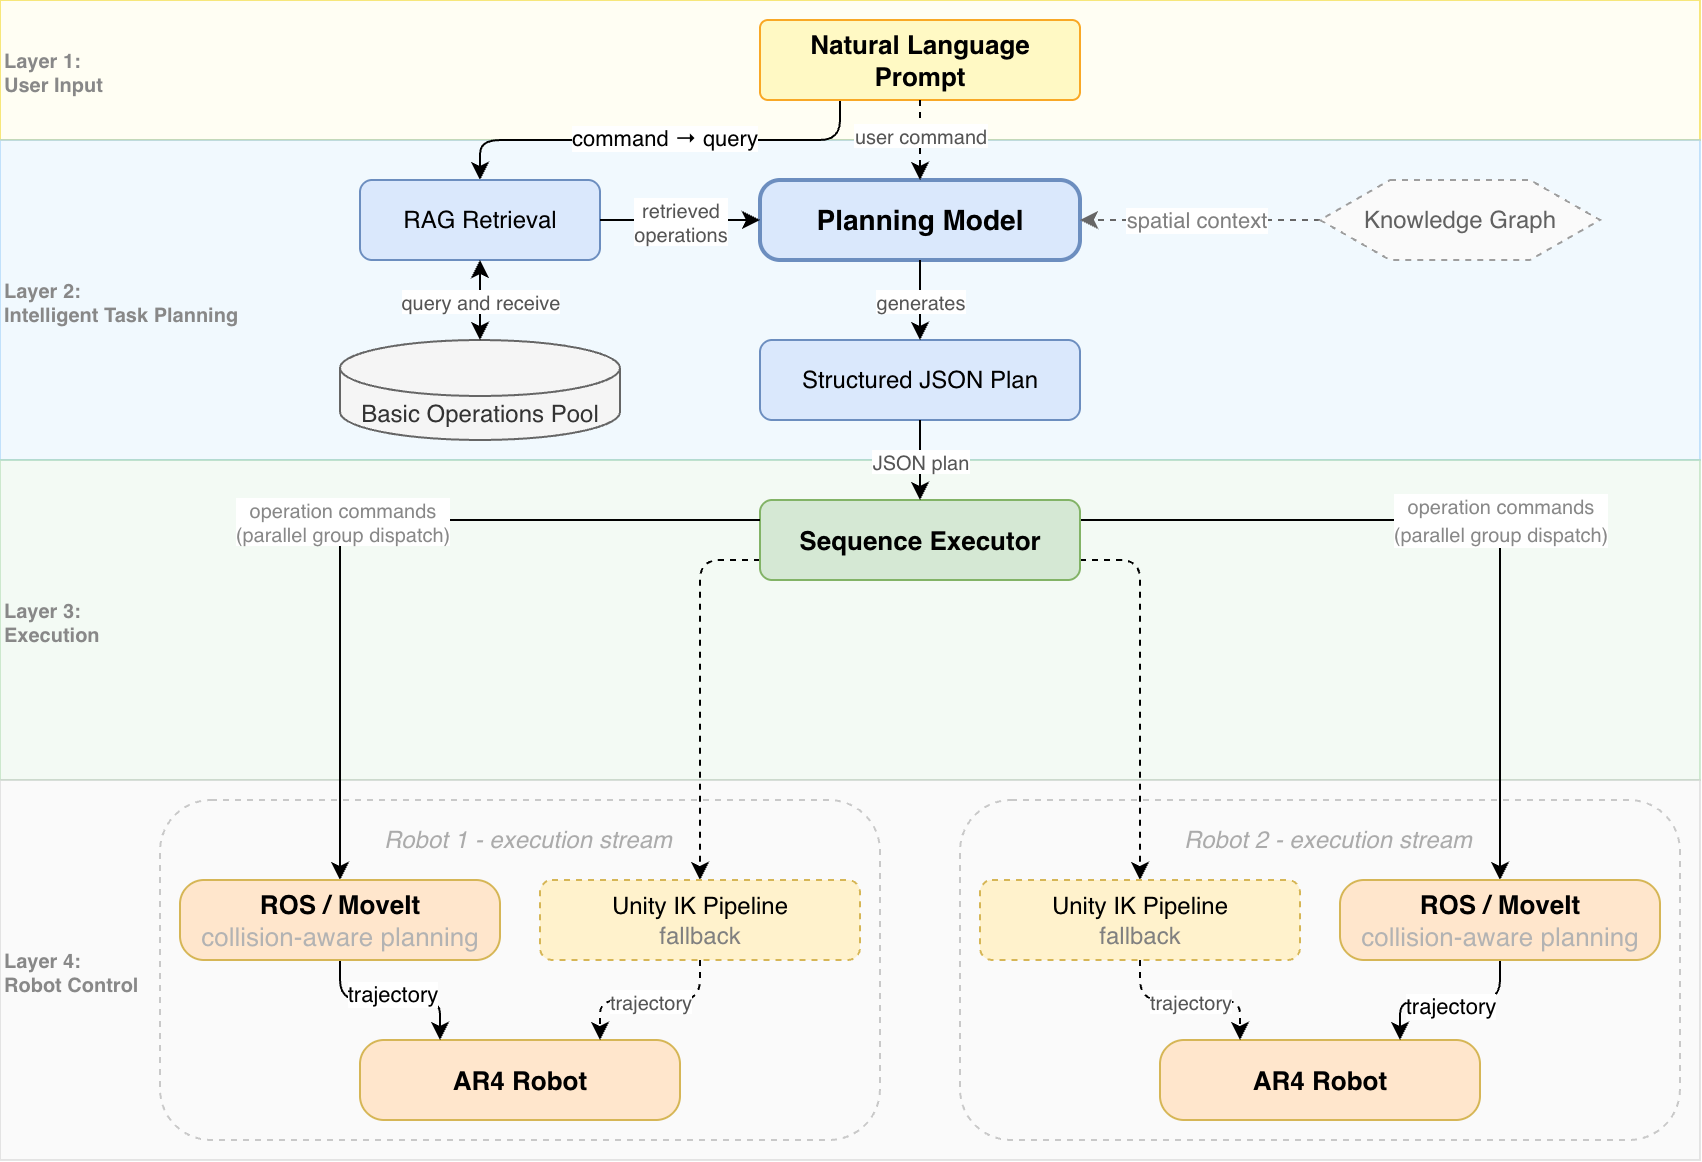
\includegraphics[width=1.0\linewidth]{images/16_system_flow.png}
	\caption{Simplified system architecture overview showing how a natural language prompt flows through the system’s four layers. Layer 1 accepts the user command and passes it to the planning layer. Layer 2 retrieves semantically relevant operations from the basic operations pool via \gls{rag}, sends them to the model, and receives a structured JSON plan. Layer 3 dispatches the plan through the sequence executor, coordinating the two robots via signal/wait synchronization and, where needed, parallel group dispatch. Layer 4 executes the resulting operation commands on the two AR4 arms through either \gls{ros}/MoveIt as a collision-aware planning backend, or the Unity \gls{ik} pipeline (dashed). The \gls{kg} provides optional spatial context to the planning layer.}
	\label{fig:system_overview}
\end{figure}

\subsection{Operations System}\label{sec:operations}
The operations system is the vocabulary the command pipeline uses. Each operation is a self-contained unit with a name, a typed parameter schema, and a structured result format. The two orthogonal axes, function and complexity level, classify them (Figure~\ref{fig:operation_map}). Below, we focus on the complexity axis because it supports failure diagnosis and tracks task difficulty. We considered a flat list, which is simplest but sacrifices failure diagnosis, and a dependency graph, which is more precise but adds complexity without practical benefit at the model-facing API level, where operations are selected by semantic intent. The level hierarchy preserves the same structural information in a form immediately useful to developers. We chose four levels because they align with real architectural boundaries:

\begin{description}
	\item[Atomic] covers single, indivisible commands with no perception dependencies and serves as a building block for higher levels.
	\item[Basic] covers simple coordinated actions that dispatch a single command and return immediately, while introducing perception, such as field detection and point-cloud generation. These also serve as building blocks for higher-level operations.
	\item[Intermediate] covers composite operations spanning object-level perception, spatial navigation, and manipulation. Its manipulation and navigation members internally invoke atomic and basic operations.
	\item[Complex] covers the task-level operations: the heaviest single-call compositions, each bundling a full perception–plan–execute pipeline for one arm, such as the grasp pipeline and the receive side of an inter-robot handoff.
\end{description}

The levels correspond to the evaluation benchmarks defined in Section~\ref{sec:benchmark-framework}. Tasks of increasing difficulty progressively exercise higher levels of the system. The practical benefit is failure diagnosis. If a Complex task fails, the developer can verify that the constituent lower-level operations succeed in isolation before investigating the composition logic. In total 20 operations are registered at startup across the four levels.

\begin{figure}
	\centering
	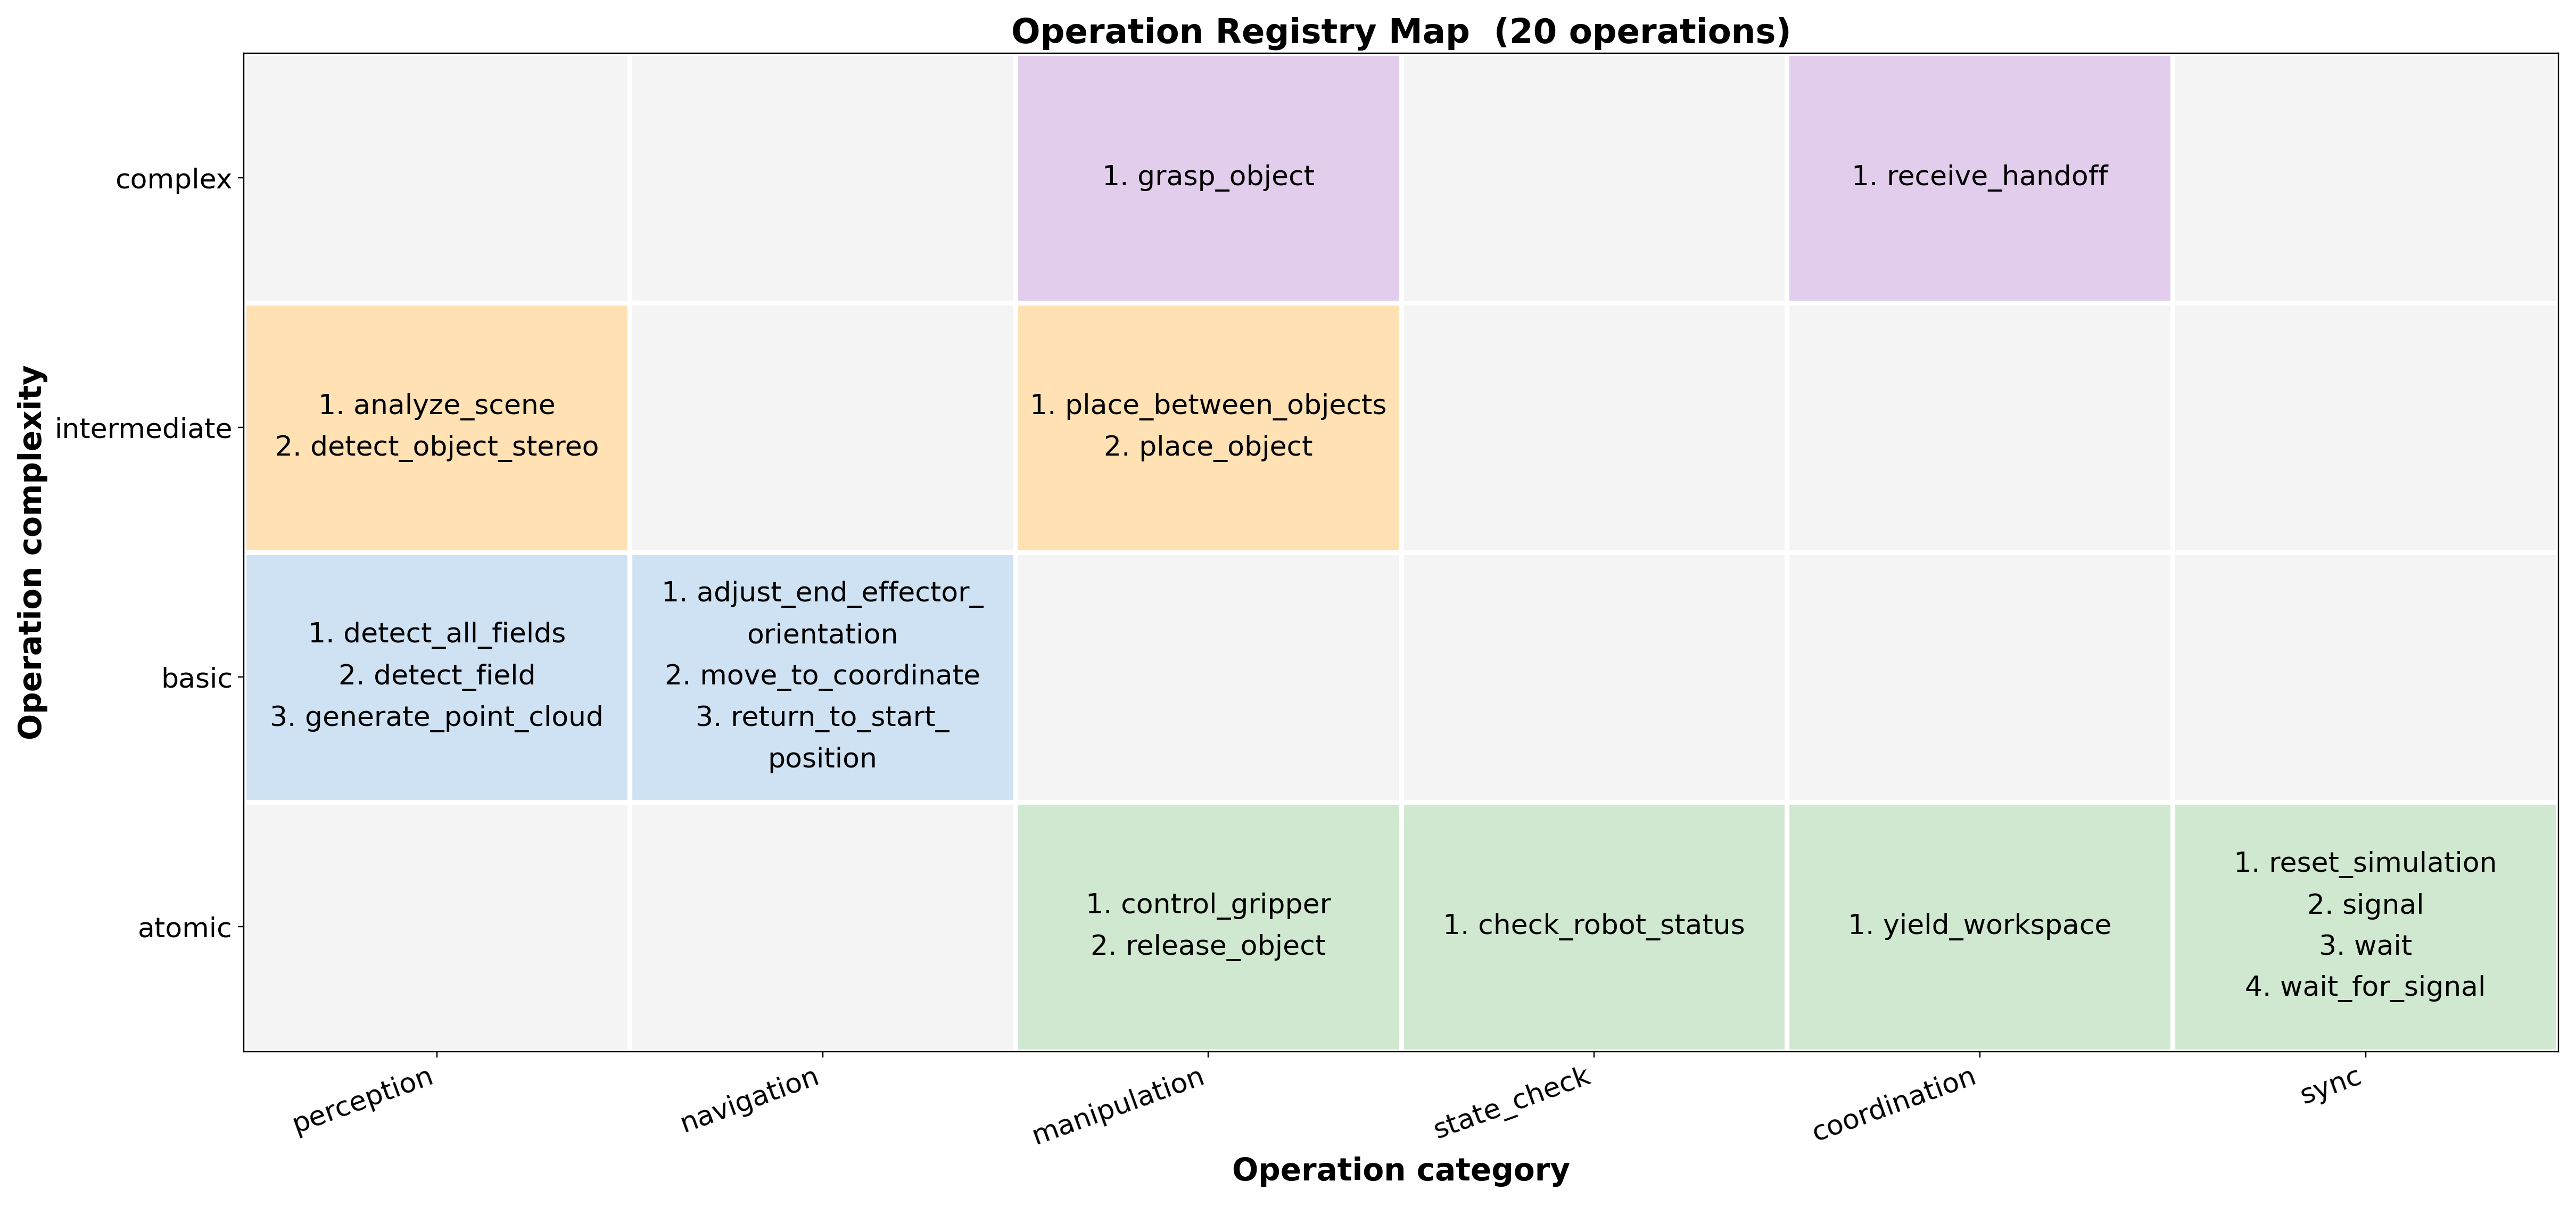
\includegraphics[width=1.0\linewidth]{images/09_operation_map.png}
	\caption{Operation registry map. The 20 operations are arranged by complexity and category.}
	\label{fig:operation_map}
\end{figure}

\subsection{Robot Operating System}\label{sec:ros}
We integrate MoveIt only as a planning backend, not as a full robot controller. This way, path computation and physical execution stay separate. MoveIt computes joint trajectories, and Unity executes them through its \texttt{ArticulationBody} physics engine. This split keeps the simulation as the single authoritative source for the robot state and eliminates the need for a \gls{ros} hardware interface or fake driver in the \gls{ros} stack. The backend is selectable at runtime depending on whether collision-aware planning is needed; Section~\ref{sec:ros_moveit} covers the control modes and their implementation.

% ------------------------------------------------------------------------------
\section{Intelligent Task Planning}\label{sec:task-planning}
Translating a natural-language instruction into robot actions requires several components working together. We describe the design of these components and how they fit together below.

\subsection{Command Pipeline}\label{sec:command-pipeline}
Our main contribution is a pipeline that takes a natural-language instruction and translates it into a coordinated sequence of robot actions. Natural language is a far more convenient interface for controlling robotic systems than writing code or browsing configuration menus, and it lowers the barrier to including robots in existing workflows. The premise is that a rich operations vocabulary reduces task planning to grounding language in structured actions. At the heart of the pipeline is a locally hosted \gls{vlm}. Its context is determined by a \gls{rag} retrieval step, so it reasons only over operations relevant to the current request. A lightweight reflection strategy recovers from transient parse failures, and an optional \gls{kg} can add spatial context. The following subsections describe each of these components in more detail.

\subsection{Local Model}\label{sec:local}
The pipeline is driven by a locally hosted reasoning model. We run it locally, which removes the dependency on cloud services and their associated costs and keeps potentially sensitive environment data off external networks, a real concern in production settings. The tasks here also do not require a frontier model; a capable, compact \gls{vlm} is sufficient. To find the most suitable option, we tested several models across parameter scales and providers. Our selection criteria were that the model must reason over visual inputs alongside text, have a moderate memory requirement, and be an open model.

\subsection{Retrieval-Augmented Generation System}\label{sec:rag}
The pipeline starts by turning the natural-language input into a vector embedding. This embedding is then used to query a vector store of all registered operations and workflow patterns via cosine similarity, retrieving the most semantically relevant ones. The retrieved operations, together with their parameter schemas, preconditions, and usage examples, are added to the \gls{vlm}’s context alongside the system prompts. It then produces a sequence of operation calls with resolved parameters, formatted as a structured JSON plan.

The key advantage of this retrieval-augmented approach over prompting the model with the full list of operations is that the model sees only operations likely relevant to the current request. Once a plan is produced, the sequence executor dispatches operations in the order specified. It threads outputs from earlier steps into later inputs, allowing instructions to be resolved at runtime without pre-specifying coordinates.

\subsection{Reflection Strategy}\label{sec:reflection}
When an operation fails, the system does not surface the error immediately; it first re-queries the model with the failure context to recover, thereby closing the perception-action loop at the language level. We based this on the verbal self-reflection traces described by Shinn \emph{et al.}~\cite{shinn2023reflexionlanguageagentsverbal}. But not all failures qualify: eligibility is restricted to operation categories where a rephrased plan can plausibly succeed.

\subsection{Knowledge Graph Integration}\label{sec:kg-integration}
The \gls{kg} is an optional layer for spatial and relational reasoning over the simulation state. Instead of querying the flat world state directly, components can ask higher-level questions, such as which robots can reach a given object, and get answers grounded in the current scene geometry. It is designed to perform spatial feasibility checks for the sequence planner before it runs multi-robot sequences. On the current task set, its measured effect is a small parse-time cost within run-to-run noise (B14, Section~\ref{sec:results-kg}), and it fails safe when absent, so it remains an optional layer whose value is expected to grow with scene complexity.

% ------------------------------------------------------------------------------
\section{Robotic Control and Coordination}
This section describes how the system manages the robot's physical motion and coordinates behavior between the two arms. It covers the multi-robot negotiation protocol, the volumetric grasping pipeline, and our adaptation of the AutoRT framework for autonomous task generation in a fixed-base manipulation setting.

\subsection{Multi-Robot Negotiation Logic}\label{sec:negotiation}
In addition to the single-model pipeline, the system includes an optional distributed negotiation protocol for multi-robot tasks, inspired by the work of Mandi \emph{et al.}~\cite{mandi2023rocodialecticmultirobotcollaboration}. Instead of a single model for both robots, each robot is assigned its own agent that reasons from its perspective. This design addresses a recurring failure. A single model coordinating two robots often under-specifies task allocations and produces plans with implicit conflicts that only surface at execution time. Distributing reasoning across agents does not eliminate this problem, but it provides a structured mechanism to surface disagreements before they lead to execution failures.

A central hub runs an analysis--proposal--evaluation cycle over up to three rounds; unanimous acceptance of a round's proposal sends the plan directly to the executor, and exhausted rounds fall back to the standard parser.

\subsection{Volumetric Grasping Network}\label{sec:vgn}
The \gls{vgn}~\cite{breyer2021volumetricgraspingnetworkrealtime} is an optional data-driven backend for 6-DOF grasp-pose prediction. While the heuristic grasp planner operates on the visible surface, \gls{vgn} takes a volumetric scene representation and predicts grasp quality, orientation, and gripper width at each point in the workspace, thereby enabling candidates to account for the full 3D geometry. Because simulated stereo degrades the network’s input, the system treats \gls{vgn}’s predicted orientation as provisional and defaults to a conservative top-down pose (Sections~\ref{sec:perception-depth} and~\ref{sec:results-vgn}).

Because single-viewpoint stereo leaves an object's occluded faces empty, its point cloud is first augmented with synthetic surface points to complete the shape, and then voxelized into the \gls{tsdf} grid on which \gls{vgn} was trained. After that, the network's ranked candidates feed the same \gls{ik} filtering and scoring stage as the heuristic planner.

\subsection{AutoRT Adaptation}\label{sec:autort}
The AutoRT framework~\cite{ahn2024autortembodiedfoundationmodels} was built for mobile robots in homes, where a robot autonomously generates tasks by observing its surroundings and proposing actions it could perform. To adapt that loop for fixed-base manipulation, we preserved the core observe, generate, filter, and execute cycle but modified several components.

Our robots have a fixed base and cannot navigate, so we dropped locomotion and exploration entirely. We re-centered the loop on object manipulation and gave the scene a more structured representation. Instead of handing the task generator raw images, the system first runs stereo object detection to obtain 3D object positions, colors, confidence levels, and graspability estimates, then uses the vision component of a \gls{vlm} to add a semantic scene summary. This formatted representation provides the generator with the object locations and graspability it needs without having to infer them from pixels.

Each iteration generates two candidate tasks, each a natural-language description with a concrete sequence of operations. The task generator runs at a higher temperature than the command parser to encourage proposal diversity. A task selector then picks one according to a configurable strategy (balanced, pure exploration, pure exploitation, or random).

Our safety filtering builds on the Robot Constitution from the AutoRT paper and is implemented here as a two-layer filter. The semantic layer, as in the paper, uses a second model call to check the proposed task against a set of safety rules. We extend this with a hard kinematic layer that the semantic layer cannot override, providing guarantees that a language model cannot: because models cannot consistently reason about physical constraints, a code-based check is the only way to prevent a task that exceeds the robot's operating envelope from reaching execution.

% ------------------------------------------------------------------------------
\section{Execution and Synchronization}
Once a plan has been validated and dispatched, the executor must manage timing and ordering across two robots. For multi-robot tasks, the pipeline uses a pair of coordination primitives so one robot can pause at a defined checkpoint until another signals completion of a prerequisite. The executor imposes no fixed coordination pattern of its own. The signal/wait primitives are general, and the model composes them according to the prompt’s synchronization and handoff rules whenever it determines synchronization is needed. The low-level robot control layer remains unaware of any higher-level coordination.

The model can also assign operations to parallel groups for concurrent dispatch. It does so by having both robots reach their positions simultaneously rather than one waiting for the other, thereby reducing the total task duration for symmetric tasks.


%%%%%%%%%%%%%%%%%%%%%%%%%%%%%%%%%%%%%%%%%%%%%%%%%%%%%%%%%%%%%%%%%%%%%%%%%%%%%%%%
%%  IMPLEMENTATION
%%%%%%%%%%%%%%%%%%%%%%%%%%%%%%%%%%%%%%%%%%%%%%%%%%%%%%%%%%%%%%%%%%%%%%%%%%%%%%%%
\chapter{Implementation}\label{implementation}
This chapter focuses on the non-trivial engineering decisions and the places where a straightforward approach failed; infrastructure that works as expected is described briefly.

\begin{figure}
	\centering
	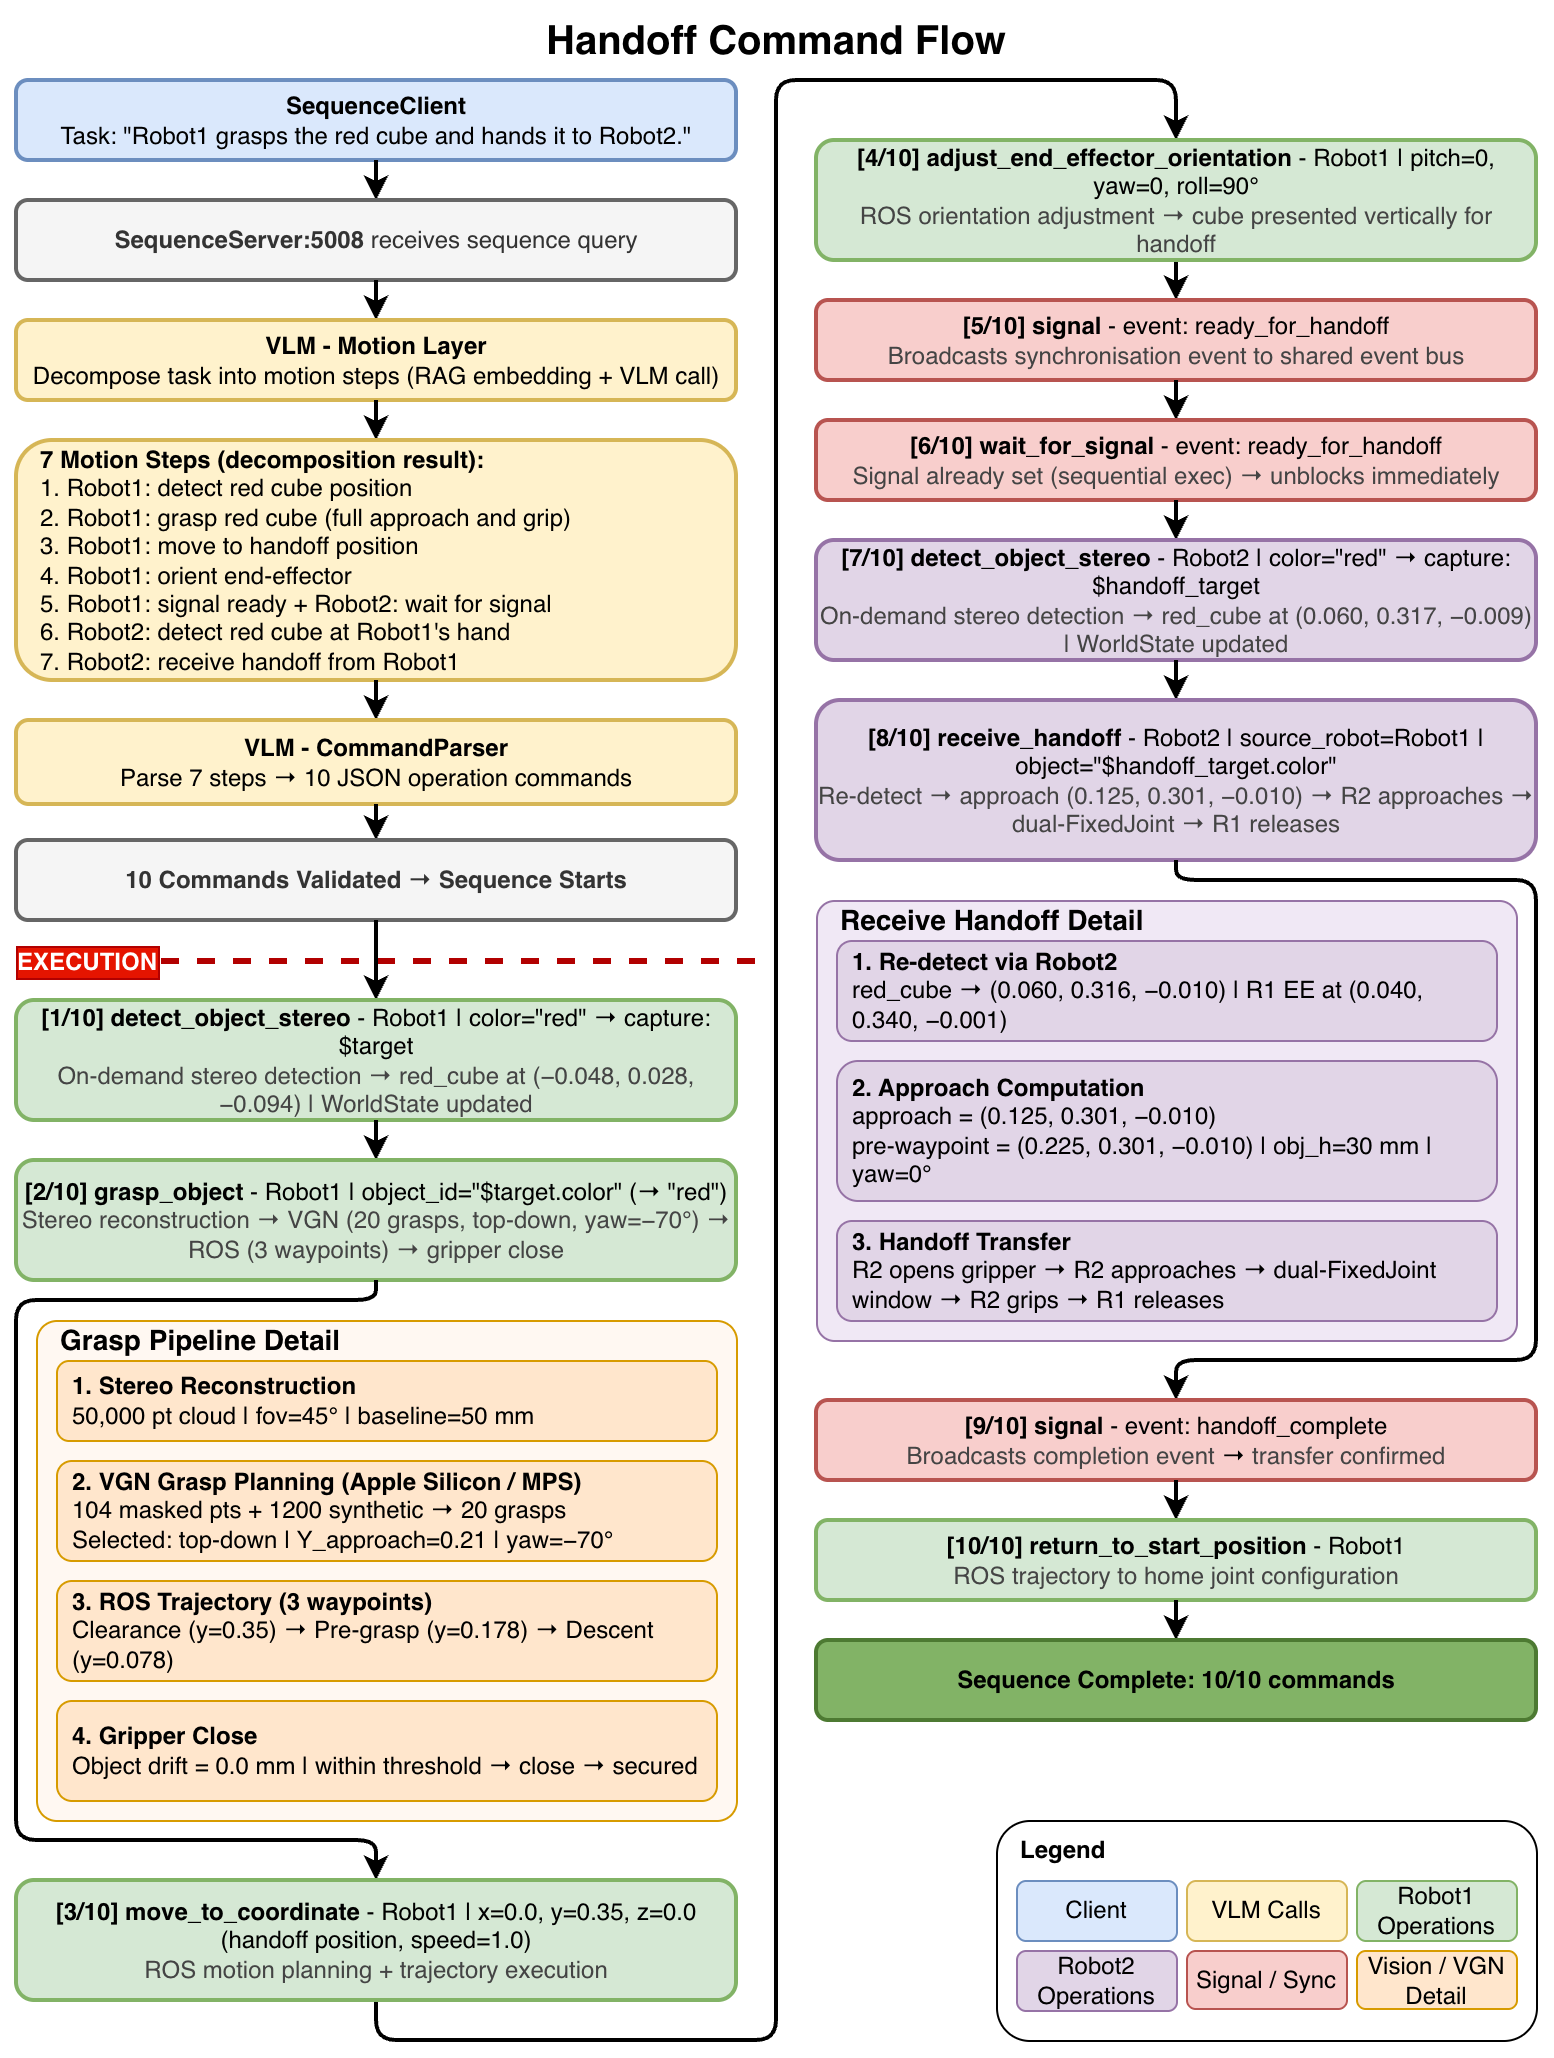
\includegraphics[width=1\linewidth]{images/12_handoff_sequence.png}
	\caption{A detailed flowgraph of how the handoff command is processed by the system.}
	\label{fig:handoff_flow}
\end{figure}

\begin{figure}
	\centering
	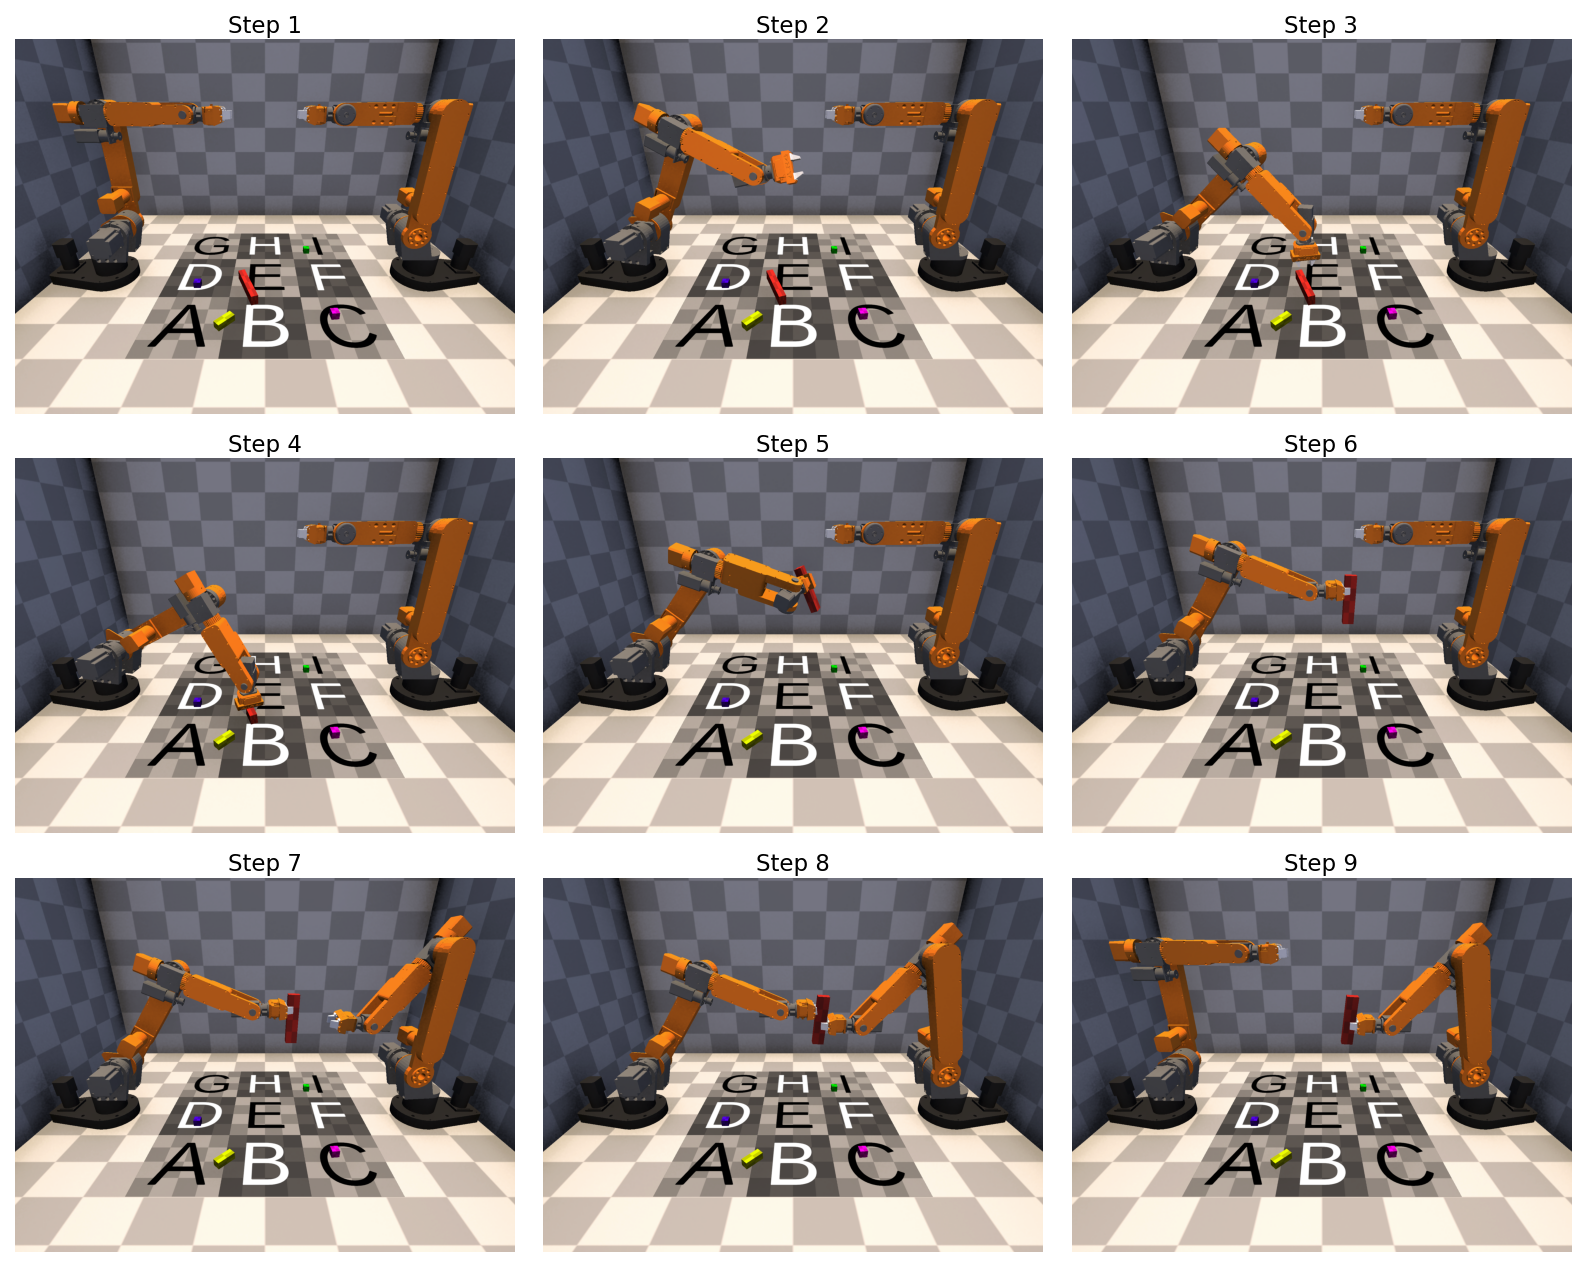
\includegraphics[width=0.75\linewidth]{images/18_handoff_sequence_example.png}
	\caption{Accompanying motion of the two robots during the handoff sequence. Note the nine steps: the \texttt{grasp\_object} and \texttt{receive\_handoff} operations each expand into internal waypoint steps.}
	\label{fig:handoff_example}
\end{figure}

Figure~\ref{fig:handoff_flow} traces a complete handoff command through most of these layers, while Figure~\ref{fig:handoff_example} shows the resulting robot motion. The flowgraph serves as a structural reference while reading this chapter, and the motion sequence illustrates the behavior the implementation produces. The full implementation is available on GitHub\footnote{\url{https://github.com/JanMStraub/Cooperative-Robot-Behavior-from-Basic-Action-Modules}}.

% ------------------------------------------------------------------------------
\section{System Infrastructure}\label{sec:infrastructure}
Before the system’s intelligent components can do anything, several foundational pieces need to be in place, especially a physics-accurate simulation environment, a motion planning backend, and a communication layer that ties Unity and Python together. The following sections describe each of these in turn, focusing on the non-obvious engineering decisions and the problems that motivated them.

\subsection{Simulation Environment and Robot Control}\label{sec:sim-env}
The simulation runs in Unity 6000.3.11f1~\cite{unity} using the \texttt{ArticulationBody} physics component to model two AR4~\cite{AnninRobotics2026} 6-DOF robotic arms (Figure~\ref{fig:robot_env}). To obtain an accurate representation of the physical robot, we imported the actual \gls{urdf} files directly into the scene. \texttt{ArticulationBody} provides reduced-coordinate dynamics, so joint behavior stays physically plausible without the numerical drift that affects traditional Rigidbody chains. Each arm is driven by a three-layer control stack, with the \gls{ik} solver at the bottom, the trajectory controller above it, and the robot controller at the top, handling convergence.

\begin{figure}
	\centering
	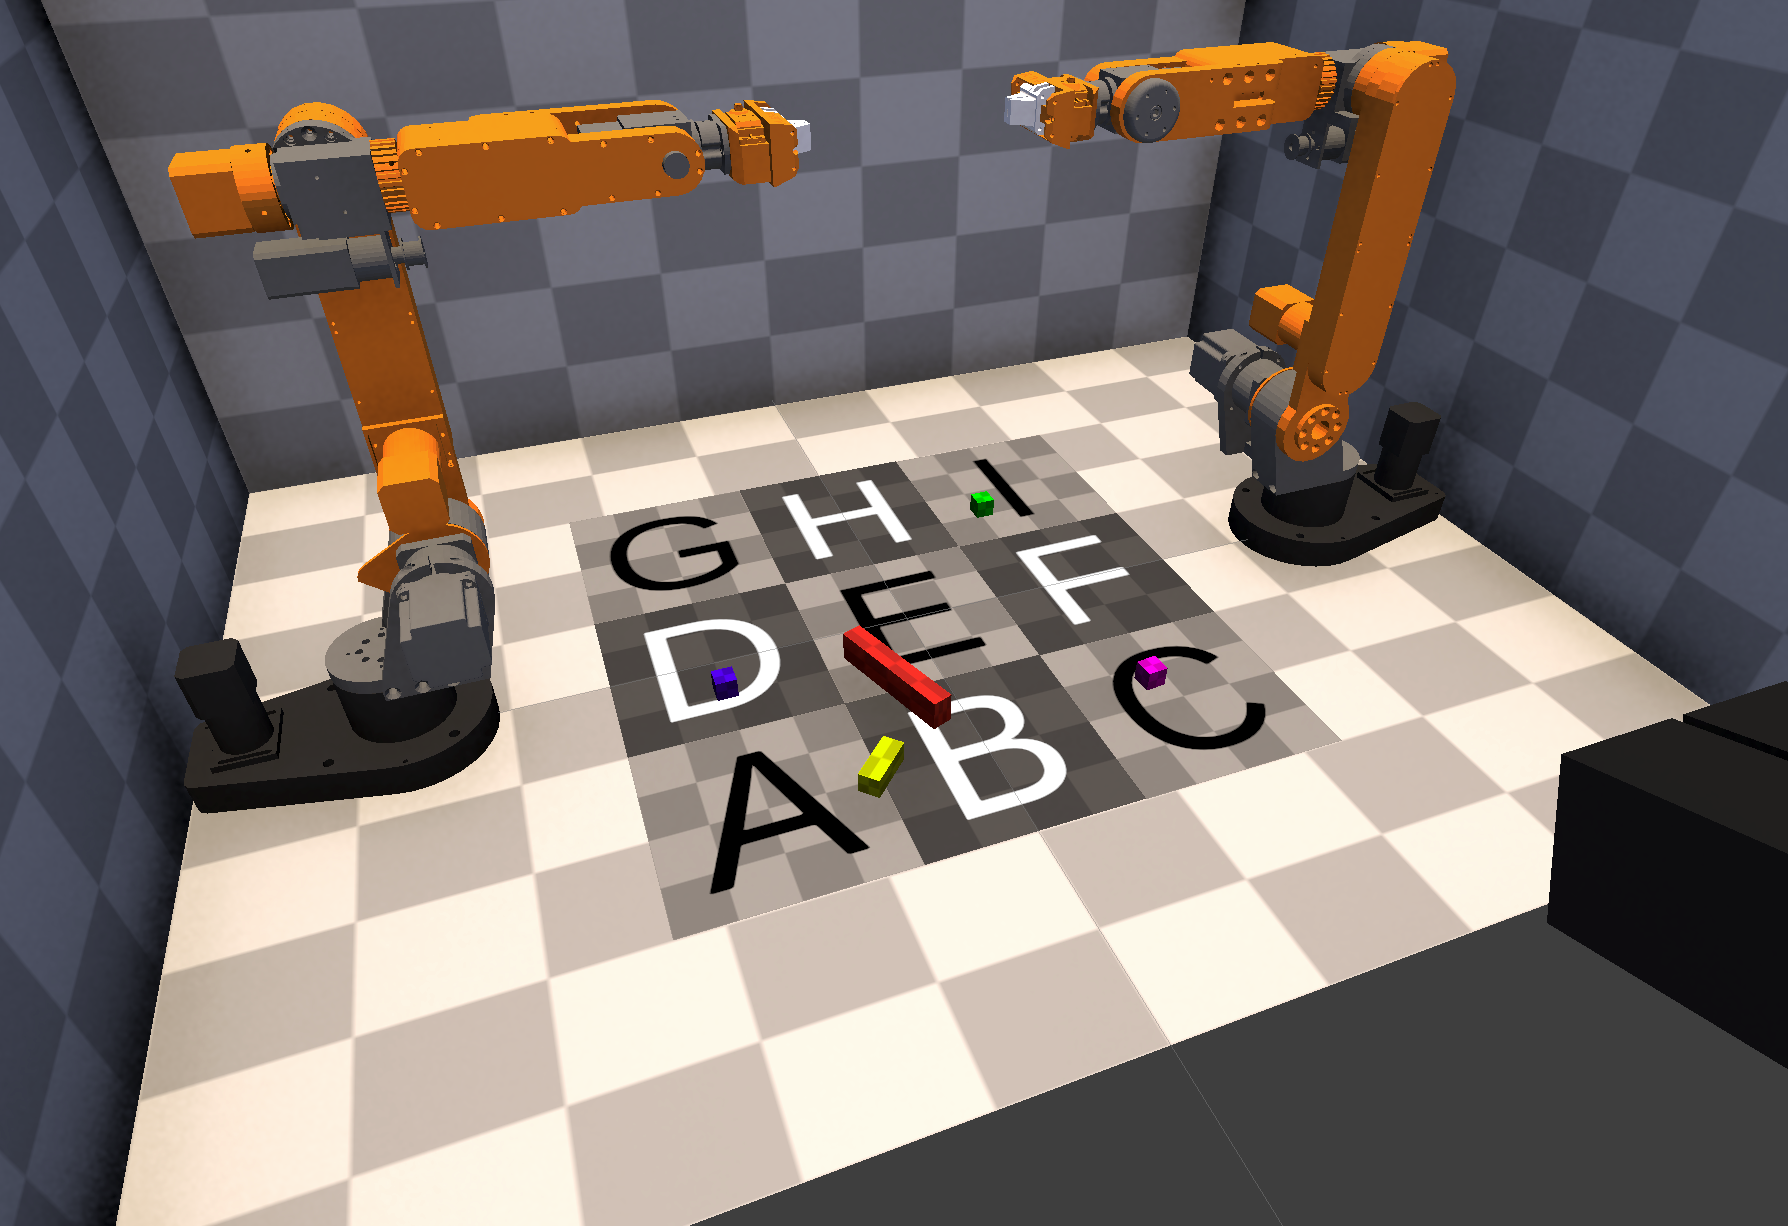
\includegraphics[width=0.5\linewidth]{images/14_robot_env.png}
	\caption{The Unity simulation environment showing the two AR4 robotic arms and the mutual workspace. Lettered zones are used to place tasks; colored objects serve as manipulation targets; and the two black boxes on the right represent the stereo camera.}
	\label{fig:robot_env}
\end{figure}

The bottom layer is the \gls{ik} solver, a damped least-squares mapping from Cartesian error to joint deltas. An earlier version oscillated due to a too-large per-frame step and insufficient damping. Adding a velocity-feedback term to the position error, turning the update into a \gls{pd} law before the damped-least-squares inverse, damped the swing. The solver maps the six-dimensional Cartesian error $e$ to a joint step $\Delta q$ through the damped pseudo-inverse
\begin{equation}\label{eq:dls}
	\Delta q = J^{\top}\bigl(J J^{\top} + \lambda^{2} I\bigr)^{-1} e,
	\qquad
	e_{\mathrm{trans}} = K_p\, e_{\mathrm{pos}} + K_d\, e_{\mathrm{vel}},
\end{equation}
where $J$ is the $6 \times n$ end-effector Jacobian, $\lambda$ the damping factor, and $I$ the identity matrix that adds $\lambda^{2}$ to the diagonal of $J J^{\top}$ to keep it invertible near singularities. The translational part of $e$ carries the \gls{pd} feedback, with $K_p$ acting on the position error $e_{\mathrm{pos}}$ and $K_d$ on its rate $e_{\mathrm{vel}}$; the rotational part is the orientation error. The translational command $K_p\, e_{\mathrm{pos}} + K_d\, e_{\mathrm{vel}}$ is clamped to unit magnitude before being combined with the orientation error and passed to the inverse, which bounds the per-step correction when a large target jump would otherwise overshoot.

We set $K_p = 3.5$ and $K_d = 0.5$. Convergence is not the solver's responsibility but the robot controller's, which declares the target reached once the position error falls below an adaptive threshold (0.02 m by default, tightened for grasping) and the orientation error is within tolerance. The remaining solver bounds are a damping factor $\lambda = 0.2$, a maximum joint step of 0.2 rad per iteration, and a joint-velocity clamp of 5.0 rad/s.

The damped least-squares solver, however, is a local, gradient-based method. It minimizes Cartesian error by following the Jacobian gradient from the current joint configuration. Because it cannot avoid local minima or reason about the global joint-space landscape, two identical Cartesian targets can produce different joint configurations and approach paths depending on the initial state, rest pose, mid-task configuration, or a previous grasp. This results in configurations near joint limits or wrist singularities that can be unreachable from some starting poses, even when they are kinematically feasible from others. Reproducibility can also suffer, as runs starting from the home pose reliably converge, while those after a sequence can land in geometrically correct but mechanically awkward configurations, increasing settling time. To fix this, multi-phase benchmarks such as B8 issue an explicit \texttt{return\_to\_start\_position} command at the end of each phase, resetting the arm to a known well-conditioned configuration before the next task.

Above the \gls{ik} solver, a trajectory controller generates trapezoidal speed curves in Cartesian space, ensuring controlled acceleration and deceleration instead of abrupt changes in target position. It operates with its own \gls{pd} gains (a position gain of 10.0 and a velocity gain of 2.0 per axis), governing how aggressively it tracks the desired profile. These gains are distinct from the \gls{ik}-level gains. The trajectory controller determines what the Cartesian target should be at any given instant, while the \gls{ik} solver translates each of those targets into joint-space commands.

We configure the \texttt{ArticulationBody} joints with per-joint stiffness and damping profiles tuned to each joint’s mechanical characteristics. Damping was tuned empirically, as the critical-damping condition $d = 2\sqrt{k \cdot I}$, where $d$ is the joint damping, $k$ the stiffness, and $I$ the rotational inertia, serves only as a lower-bound reference; at Unity’s 50~Hz physics rate, the joints require damping well above this baseline (see Appendix~\ref{appendix:robot_values}).

This three-layer control stack is only fully active in Unity mode. In the default Hybrid mode, each motion is attempted through MoveIt first and falls back to the Unity \gls{ik} and trajectory stack when planning fails, for instance, on a wrist singularity or an unreachable goal. In \gls{ros} mode, MoveIt computes every joint trajectory, Unity receives it over the \gls{ros}-TCP bridge, and the \texttt{ArticulationBody} joints execute it directly; the \gls{ik} solver and trajectory controller are bypassed entirely. The \gls{ros} implementation is described in detail in Section~\ref{sec:ros_moveit}.

\begin{figure}
	\centering
	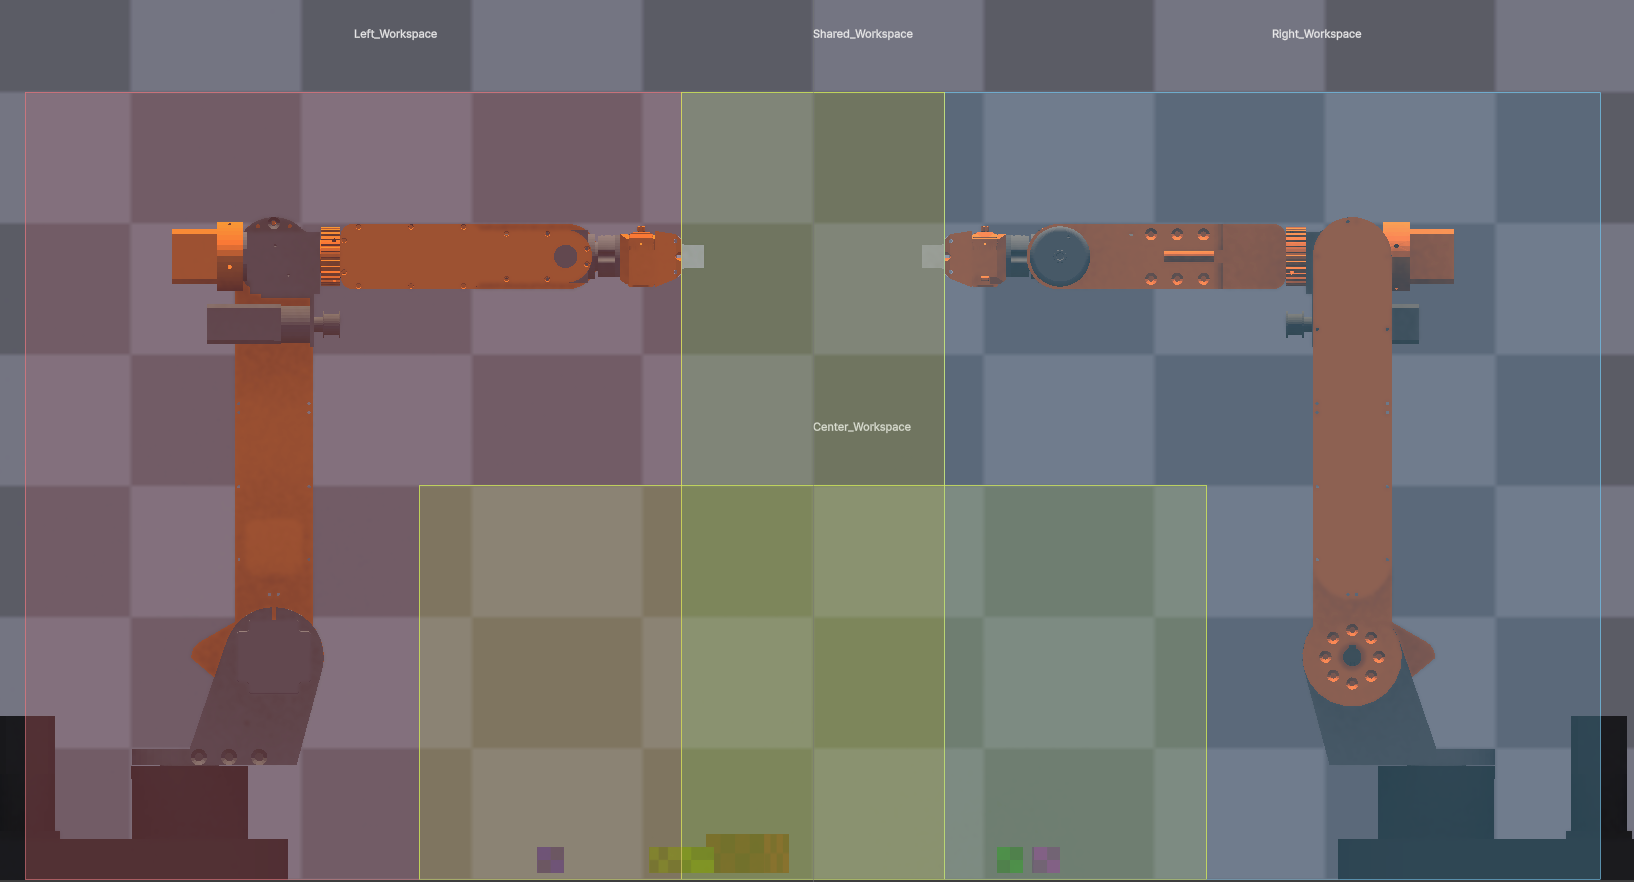
\includegraphics[width=0.75\linewidth]{images/15_robot_workspaces.png}
	\caption{Workspace regions defined in Unity, used by the \gls{kg} and the evaluation benchmarks. Red and blue mark each robot’s primary zone; the yellow areas are the center and shared zones where the two arms may interact.}
	\label{fig:robot_workspaces}
\end{figure}

Safety limitations operate in three distinct layers. At the Python level, \texttt{CoordinationVerifier} runs a static pre-check before every navigation command. If the planned target falls within 60~mm of the partner robot’s current end-effector position, the command is blocked, and a safe waypoint is prepended to the resolution suggestions before dispatch. When both robots are moving, a separate, looser check compares the two planned targets to ensure a minimum separation of 0.2~m. The same pass also checks for workspace conflicts, object conflicts (both robots targeting the same grasped object), and potential deadlocks.

At the Unity level, the \texttt{ProximityGuard} monitors end-effector separation at runtime. When their separation drops below 0.25~m, both robots freeze. Link-to-link proximity for joints 2–5 is assessed separately using a tighter 0.15~m threshold, since mid-arm collisions can occur even when end-effectors are far apart. The frozen state is broadcast to Python on the next \texttt{WorldStatePublisher} cycle, allowing the planner to replan. During intentional close-approach operations such as handoffs, the \texttt{ProximityGuard} is disabled by the \texttt{receive\_handoff} operation and re-enabled on completion, because those sequences handle inter-robot safety internally through the signal/wait serialization protocol.

The third safety layer is the workspace region system (Figure~\ref{fig:robot_workspaces}). The workspace is divided into four named regions: \texttt{left\_workspace} ($-0.6 \leq x \leq -0.1$~m, Robot~1’s main area), \texttt{right\_workspace} ($0.1 \leq x \leq 0.6$~m, Robot~2’s main area), \texttt{shared\_zone} ($-0.1 \leq x \leq 0.1$~m, the overlap of both robots’ allocations), and \texttt{center} (which overlaps the shared zone and inner parts of both workspaces and is used by the \gls{kg} for proximity reasoning). Region ownership is tracked by Python’s \texttt{WorldState}. Enforcement occurs through the \texttt{yield\_workspace} operation, which causes a robot to release its current region so the partner may enter. This strict region partition differs from the per-robot reachability bounds provided to the command-parser model in its prompt (Appendix~\ref{appendix:prompts}), which extend each arm's reachable range to $|x| \leq 0.165$~m. The difference is that the looser bound reflects the actual kinematic reach across the centerline, so the model can place and grasp objects there, while the tighter $\pm0.1$~m \texttt{shared\_zone} sets the conservative boundary at which region allocation and coordination take over.

\subsection{Grasp Planning Pipeline}\label{sec:grasp-pipeline}
Grasping is handled by a four-stage pipeline inspired by the MoveIt grasp planning architecture and implemented separately on both the Unity and Python sides. The two implementations share the same logical structure, namely candidate generation, \gls{ik} filtering, collision filtering, and scoring, but they serve different execution paths. The Unity pipeline plans for the built-in \gls{ik} stack, while the Python pipeline plans for the \gls{ros}/MoveIt path and validates its candidates directly against MoveIt’s \gls{ik} solver. Table~\ref{tab:grasp_params} lists the key parameter differences.

\begin{table}[t]
	\centering
	\begin{tabular}{lcc}
		\hline
		\textbf{Parameter}             & \textbf{Unity} & \textbf{Python} \\
		\hline
		Candidates per direction       & 10             & 8               \\
		Angle perturbation             & $\pm20^\circ$  & $\pm15^\circ$   \\
		Maximum reach                  & 0.6 m          & 0.75 m          \\
		\gls{ik} validation iterations & 250            & 50              \\
		\gls{ik} validation threshold  & 0.01 m         & 0.005 m         \\
		Depth score weight             & 0.6            & 1.0             \\
		Pipeline time budget           & 1000 ms        & 200 ms          \\
		\hline
	\end{tabular}
	\caption{Grasp planning parameters for the Unity (\texttt{GraspConfig.asset}) and Python (\texttt{grasp\_planning/GraspConfig.py}) implementations. We tuned the Unity values for PhysX execution. A generous \gls{ik} budget and a tighter 0.6~m reach keep candidates within the range where the damped least-squares solver converges reliably. The Python pipeline can afford a tighter validation threshold and shorter time budget because its candidates are checked against MoveIt’s \gls{ik} solver.}
	\label{tab:grasp_params}
\end{table}

The candidate generator produces proposals for three directions: top, front, and side. It uses approach-angle perturbations and object-size-adaptive pre-grasp distances ranging from 5 to 15 cm. Candidates pass through an \gls{ik} filter that first applies a fast distance-based reachability check and then a full \gls{ik} validation. Those that survive are evaluated by a collision filter, which samples five waypoints along the approach trajectory and performs sphere-cast checks within a 3 cm radius at each waypoint. The final scorer combines five weighted additive criteria, namely \gls{ik} quality (weight 1.0), approach direction preference (0.8), grasp depth relative to the object center (0.6 Unity / 1.0 Python), stability based on contact geometry (1.2), and antipodal quality (1.0), all scaled by an orientation-consistency multiplier. We gave the stability term the highest weight because empirical tuning showed it was the strongest predictor of whether the grasp would withstand the forces encountered during subsequent manipulation.

Grasp verification after closing is handled by a contact sensor. It tracks per-finger contact via Unity’s collision callbacks, applies a 5-frame moving average to smooth physics noise, and requires a minimum contact duration of 50~ms and an estimated contact force above 5~N before declaring a successful grasp.

The \gls{vgn} pipeline~\cite{breyer2021volumetricgraspingnetworkrealtime} is an optional learned backend for 6-DOF grasp-pose prediction, retained as sim-to-real infrastructure and not the currently active alternative to the heuristic planner. It takes a \gls{yolo} bounding box, constructs a masked point cloud, builds a \gls{tsdf} volume, and runs \gls{vgn} inference to produce 6-DOF grasp poses, which are injected into the same filter and scorer pipeline. The executed orientation, however, is a top-down override described below, while the grasp position is taken from the detected object center. In this simulation, the center is supplied by the \texttt{WorldState} oracle rather than recovered from the point cloud, since the per-pixel depth needed to localize it from stereo is unreliable on Unity's textureless surfaces (Section~\ref{sec:perception-depth}). The measurable benefit of enabling the \gls{vgn} path therefore comes from this positioning, not from \gls{vgn}'s predicted pose (Section~\ref{sec:results-vgn}).

We first tried Contact-GraspNet~\cite{sundermeyer2021contactgraspnetefficient6dofgrasp} as the data-driven backend. However, it requires a dedicated GPU for inference, which we did not have in our development environment, so we adopted \gls{vgn} instead. Its lighter inference footprint runs on the CPU and Apple Silicon without modification, aligning with the infrastructure-independent deployment goals in Section~\ref{sec:local}. Although \gls{vgn} is trained on both top-down and side grasps, the sparse \gls{tsdf} volumes produced by this system’s stereo disparity rarely yield a confident near-vertical prediction. Our pipeline, therefore, imposes a top-down orientation unless \gls{vgn}'s predicted approach is strongly vertical ($|Y| \geq 0.7$); otherwise, the predicted approach is discarded and replaced with a straight-down grasp whose yaw is derived geometrically from the object’s long axis. Under this system’s stereo depth, the threshold is seldom met, so most executed grasps are top-down by override, not \gls{vgn}'s own preference.

\subsection{Robot Operating System and MoveIt Integration}\label{sec:ros_moveit}
The key implementation choice is to enable the \texttt{plan\_only} flag in the MoveGroup goal. MoveIt produces a joint trajectory plan but does not attempt to execute it, and Unity receives it over the \gls{ros}-TCP bridge and runs it through its \texttt{ArticulationBody} physics. The rationale for this planning-only split is given in Section~\ref{sec:ros}.

The three control modes introduced in Section~\ref{sec:sim-env} vary mainly in planning cost and collision handling. \gls{ros} mode plans through MoveIt, with trajectory execution averaging about 5~s per motion (Table~\ref{tab:b16-results}), and it provides full collision-aware planning via \gls{ompl}~\cite{6377468}. Unity mode is preferable when lower latency is required, and collision-aware planning is not needed, while \gls{ros} mode becomes worthwhile once the workspace is cluttered enough to need collision-free planning; Hybrid, the default, blends the two.

Joint states are published at 50~Hz using pre-allocated \gls{ros} messages to avoid garbage-collection pressure. Trajectories are received and validated against joint limits and velocity constraints. They are then interpolated to Unity’s fixed-update frequency. In dual-robot mode, all topics are namespaced per robot to keep the two control streams independent.

We encountered three failure modes during integration. Each required an explicit fix before the \gls{ros}/MoveIt path became reliable.

\paragraph{MoveIt \texttt{UNKNOWN\_ERROR\_99999}.}
\gls{ompl} aborted planning with error code 99999 in two distinct scenarios. First, Unity’s \texttt{ArticulationBody} physics can overshoot joint limits at the end of a trajectory, particularly after a settle timeout. Because those out-of-bounds values were submitted as the MoveIt start state, \gls{ompl} rejected it as kinematically invalid; our fix clamps every joint value to its \gls{urdf} bounds before constructing the \texttt{RobotState} message. Second, setting \texttt{is\_diff = false} at the start state caused unlisted joints to default to zero, placing the robot in self-collision or in contact with the ground plane and triggering the same error. Setting \texttt{is\_diff = true} instructs MoveIt to apply the provided joints as a differential update over its internally tracked state, leaving unlisted joints unchanged. Additionally, gripper jaw joints published by Unity must be stripped from the start state prior to submission, because the \texttt{arm} planning group does not include them, and their presence renders the start state invalid.

\paragraph{Execution settle timeout.}
Unity sends a \texttt{completed\_with\_timeout} status when trajectory execution finishes, but the arm has not fully settled at its drive target within the allotted window. If the next plan is requested immediately, MoveIt receives a stale \texttt{/joint\_states} that still reflects the arm mid-motion, resulting in a start state that either violates joint bounds or is in an unexpected configuration. Our fix inserts a 3~s physics-settle wait after any \texttt{completed\_with\_timeout} response before the next planning request is issued. The execution timeout itself is set dynamically as
\begin{equation}
	t_{\mathrm{exec}} = \max\bigl(c_0,\; 2.5 \cdot t_{\mathrm{traj}} + c_1\bigr)~\text{s},
\end{equation}
where the floor $c_0$ and offset $c_1$ are set per call path (for example, $c_0 = 30$, $c_1 = 15$ on the primary plan-and-execute path), so the timeout scales conservatively with trajectory duration.

\paragraph{\gls{vgn} approach bias.}
When stereo point cloud quality is insufficient to produce reliable \gls{tsdf} input, \gls{vgn}'s predicted approach vectors bias toward the horizontal; selecting the highest-scoring candidate unfiltered then rotates the wrist into a twisted configuration that the planner rejects. The fix is the $|Y| \geq 0.7$ vertical-component threshold described above. Near-vertical predictions are trusted; all others are overridden with the top-down direction.

\subsection{Communication Architecture}\label{sec:communication}
The Unity simulation and the Python backend communicate over TCP. All messages use a protocol that prepends a 5-byte header to each message: one byte for the message type and four bytes for the request identifier. The request ID enables asynchronous request-response matching. The Python backend maintains per-request queues and handles concurrent operations from multiple robots without mixing replies.

World state is published on a dedicated port as a one-way broadcast stream with a fixed request ID of zero, explicitly separating it from the request–response channel. We introduced this separation after early versions suffered correlation errors. High-frequency world-state updates arrived interleaved with command responses.

End-to-end, a command flows as follows. A natural-language sequence arrives at the Python \texttt{SequenceServer}; the backend passes it to the command parser; the parsed plan is sent to the sequence executor, which dispatches each operation via the \gls{ros}-Unity router. In the default Hybrid mode, motion commands are planned by MoveIt and the resulting trajectory is executed by Unity through its \texttt{ArticulationBody} physics. If planning fails, the system falls back to the Unity \gls{ik} pipeline. Unity then returns a completion notification. In practice, model parsing is the dominant fixed cost. The median time from query arrival to a validated plan was roughly 20~s, limited by the reasoning model’s thinking budget. Motion planning adds well under 0.5~s on the \gls{ros} path, or 5–10~ms per \gls{ik} step on the Unity path. Robot movement adds 2–10~s per motion command, depending on travel distance, so a single-robot command sequence typically finishes within 30–60~s of arriving, while dual-robot handoff sequences extend to roughly 60–100~s.

On top of this TCP backbone sits an optional operator interface, the Mission Control dashboard. It acts purely as a client of the existing backend. It renders the live scene from the world-state broadcast, streams logs and AutoRT task proposals, accepts natural-language commands, and exposes the benchmark analysis tab used in Chapter~\ref{evaluation}.

% ------------------------------------------------------------------------------
\section{Operations System}\label{sec:ops-impl}
Each operation is an instance of the \texttt{BasicOperation} dataclass, configured with an implementation callable; its shared \texttt{execute()} method validates parameters and dispatches to that callable, returning an \texttt{OperationResult} containing a success flag, an optional error dictionary, and a result dictionary. Operations are registered in a central registry at startup, which serves as the single source of truth for the \gls{rag} indexer, the command parser prompt, and the AutoRT task generator.

Beyond the operation implementations themselves, each operation carries structured metadata that the \gls{rag} system actively uses. \texttt{ParameterFlow} objects declare how output fields of one operation map onto input parameters of another, allowing the retrieval step to surface both the most relevant individual operation and the natural sequences it belongs to. Seven such flows are defined across the registry, covering vision, field, and spatial operations. In addition, \texttt{OperationRelationship} objects declare which operations are commonly paired together and what temporal ordering constraints exist between them.

An example of an operation can be found in Appendix~\ref{appendix:operation_example}.

% ------------------------------------------------------------------------------
\section{Intelligent Task Planning}\label{sec:planning-impl}
This section covers the concrete implementation of the command pipeline described in Section~\ref{sec:command-pipeline}, covering how we serve and configure the local model, build and query the \gls{rag} index, and convert a retrieved plan into robot actions.

\subsection{Local Model Selection}
The locally hosted \gls{vlm} is served via LM Studio~\cite{lmstudio}, which exposes an OpenAI-compatible API endpoint. We chose this interface because it lets the same client code target different models without modification, making model substitution straightforward during evaluation. Temperature is set to 0.3 for command parsing, low enough to keep plan generation predictable. For multi-step tasks, we use two complementary mechanisms to improve output quality. The first is a model-level thinking block, enabled via LM Studio’s \texttt{budget\_tokens} parameter, that lets the model reason internally before producing a response; the second is a chain-of-thought context injected into the prompt as motion-planning guidance. Together, these reduce structural errors in the generated plans, though we have not independently measured the effect of each mechanism.

\subsection{Retrieval-Augmented Generation System and Embedding}
Embeddings are generated using \texttt{nomic-embed-text-v1.5}~\cite{nussbaum2025nomicembedtrainingreproducible}, served locally via LM Studio and producing 768-dimensional vectors. The vector store uses cosine similarity search with an in-memory index protected by a thread-safe lock; the index is persisted to disk, so re-indexing is needed only when operations change. Query results are filtered using a minimum similarity threshold of 0.5 and a configurable confidence strategy (strict/balanced/permissive). If LM Studio is unavailable at startup, the system falls back to \gls{tfidf} with a maximum of 500 features, which is coarser, but sufficient to keep the system functional in degraded conditions. Figure~\ref{fig:rag} shows the indexing and search pipeline.

\begin{figure}
	\centering
	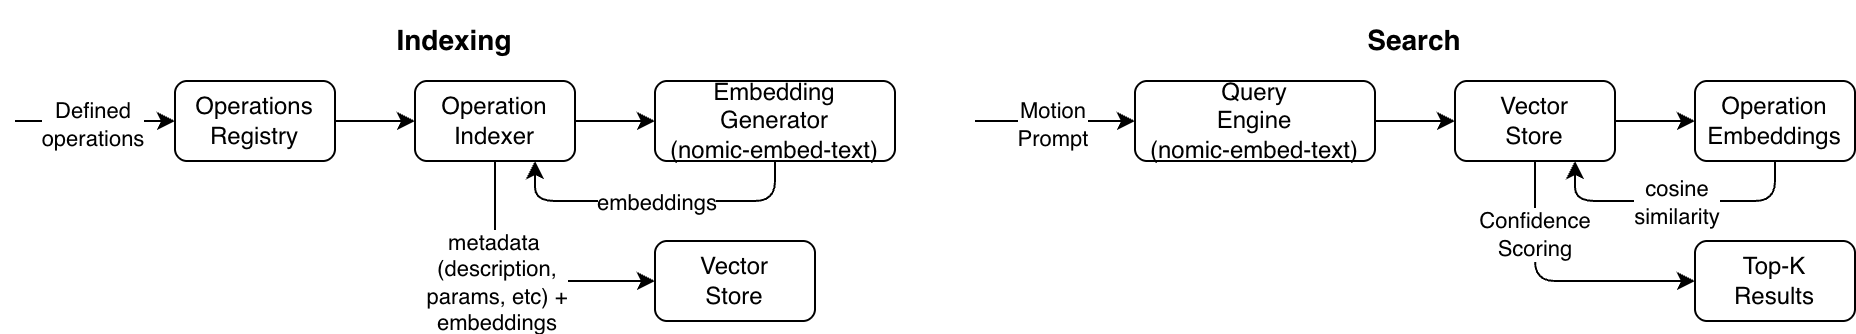
\includegraphics[width=1\linewidth]{images/13_rag.png}
	\caption{Indexing and search in the \gls{rag} system: operations are embedded and stored at startup (left); a user prompt is embedded and matched by cosine similarity, then confidence-scored to Top-K results (right).}
	\label{fig:rag}
\end{figure}

The \gls{rag} index contains 31 items in total: the 20 registered operations, 7 predefined workflow patterns, and 4 multi-robot context documents. The workflow patterns describe common multi-step sequences in a structured format, including pattern-level success criteria and failure recovery hints. When one pattern scores highly during retrieval, it is injected into the model prompt as an example plan, reducing structural errors in generated plans for familiar task types. The context documents cover workspace layout, coordination patterns, safety restrictions, and parallel execution guidelines, providing the model with relevant background when no single operation is a close semantic match for the query.

\subsection{Command Parser and Sequence Executor}
The command parser extracts and normalizes the JSON from the model’s response. Per request, a 90-second timeout is applied, and a connection pool with 10 persistent connections reduces TCP overhead. The system prompt lists the top \gls{rag}-retrieved operations with their full parameter schemas. The vector store is queried for 10 candidates spanning both operations and workflow patterns. These candidates are partitioned by type; up to 5 operations and up to 3 workflow patterns are retained, and any surplus is discarded. The most relevant items, together with critical rules for multi-robot tasks and the variable-passing syntax, are then fed into the prompt.

Before execution, the parser validates the returned plan. Operation names are checked against the registry, and every \texttt{wait\_for\_signal} call must have a matching \texttt{signal} with the same identifier. Variable references are resolved at execution time; unresolved references fall back to recovery patterns or are left for the operation’s parameter type-check to reject, and missing \texttt{capture\_var} declarations are inferred from downstream \texttt{\$var} usage. If the response can be partially salvaged, for example, if the model returned a bare array instead of a wrapped object, a normalization step is attempted before returning an error. If LM Studio~\cite{lmstudio} is entirely unreachable, the parser falls back to a regex-based matcher that covers a subset of common command patterns.

The sequence executor iterates over the validated plan. For operations sharing the same parallel group identifier, it dispatches them concurrently and blocks until all complete or a timeout elapses. Variable passing is handled automatically. After each operation, result fields declared in the operation’s parameter flow metadata are stored in a session-scoped variable dictionary; before each operation, missing parameters are filled from this dictionary by field-name matching. Both explicit capture directives in the plan and automatic capture run in sequence, with explicit directives applied first. Signal and wait primitives are implemented using a \texttt{threading.Condition} variable. The signaling robot calls \texttt{notify\_all()} on the condition, and the waiting robot blocks on the condition until notified.

\subsection{Reflection Strategy}\label{sec:reflection-impl}
When an operation fails, the executor checks whether it qualifies for reflection-based recovery. Only Navigation, Manipulation, and Perception operations are eligible; synchronization primitives and status checks are explicitly excluded, since re-querying the language model for them offers no benefit and adds latency. If the failed operation is eligible and reflection is enabled, the executor constructs a failure hint by combining the error message with any recovery suggestions returned by the failed operation. This hint is returned to the command parser alongside the original natural-language command, which re-queries the \gls{vlm} with the failure context appended. The re-parsed command is re-resolved against the current variable store and re-executed. By default, this loop runs up to 2 retries; on success, the failed entry in the sequence log is replaced with the successful result, and execution continues normally.

\subsection{Knowledge Graph}\label{sec:kg-impl}
The \gls{kg} is implemented as a thread-safe directed multi-graph that permits safe access from the world-state callback thread and from operation handlers. The graph is updated in place on every world-state update by a builder that registers as a callback on the world-state server. Three node types represent robots, objects, and workspace regions. Six edge relations are actively populated: \textsc{Can\_Reach}, \textsc{Near}, \textsc{In\_Region}, \textsc{Grasping}, \textsc{Adjacent\_To}, and \textsc{Allocated}. Figure~\ref{fig:kg_example} shows the graph state at simulation start.

\begin{figure}
	\centering
	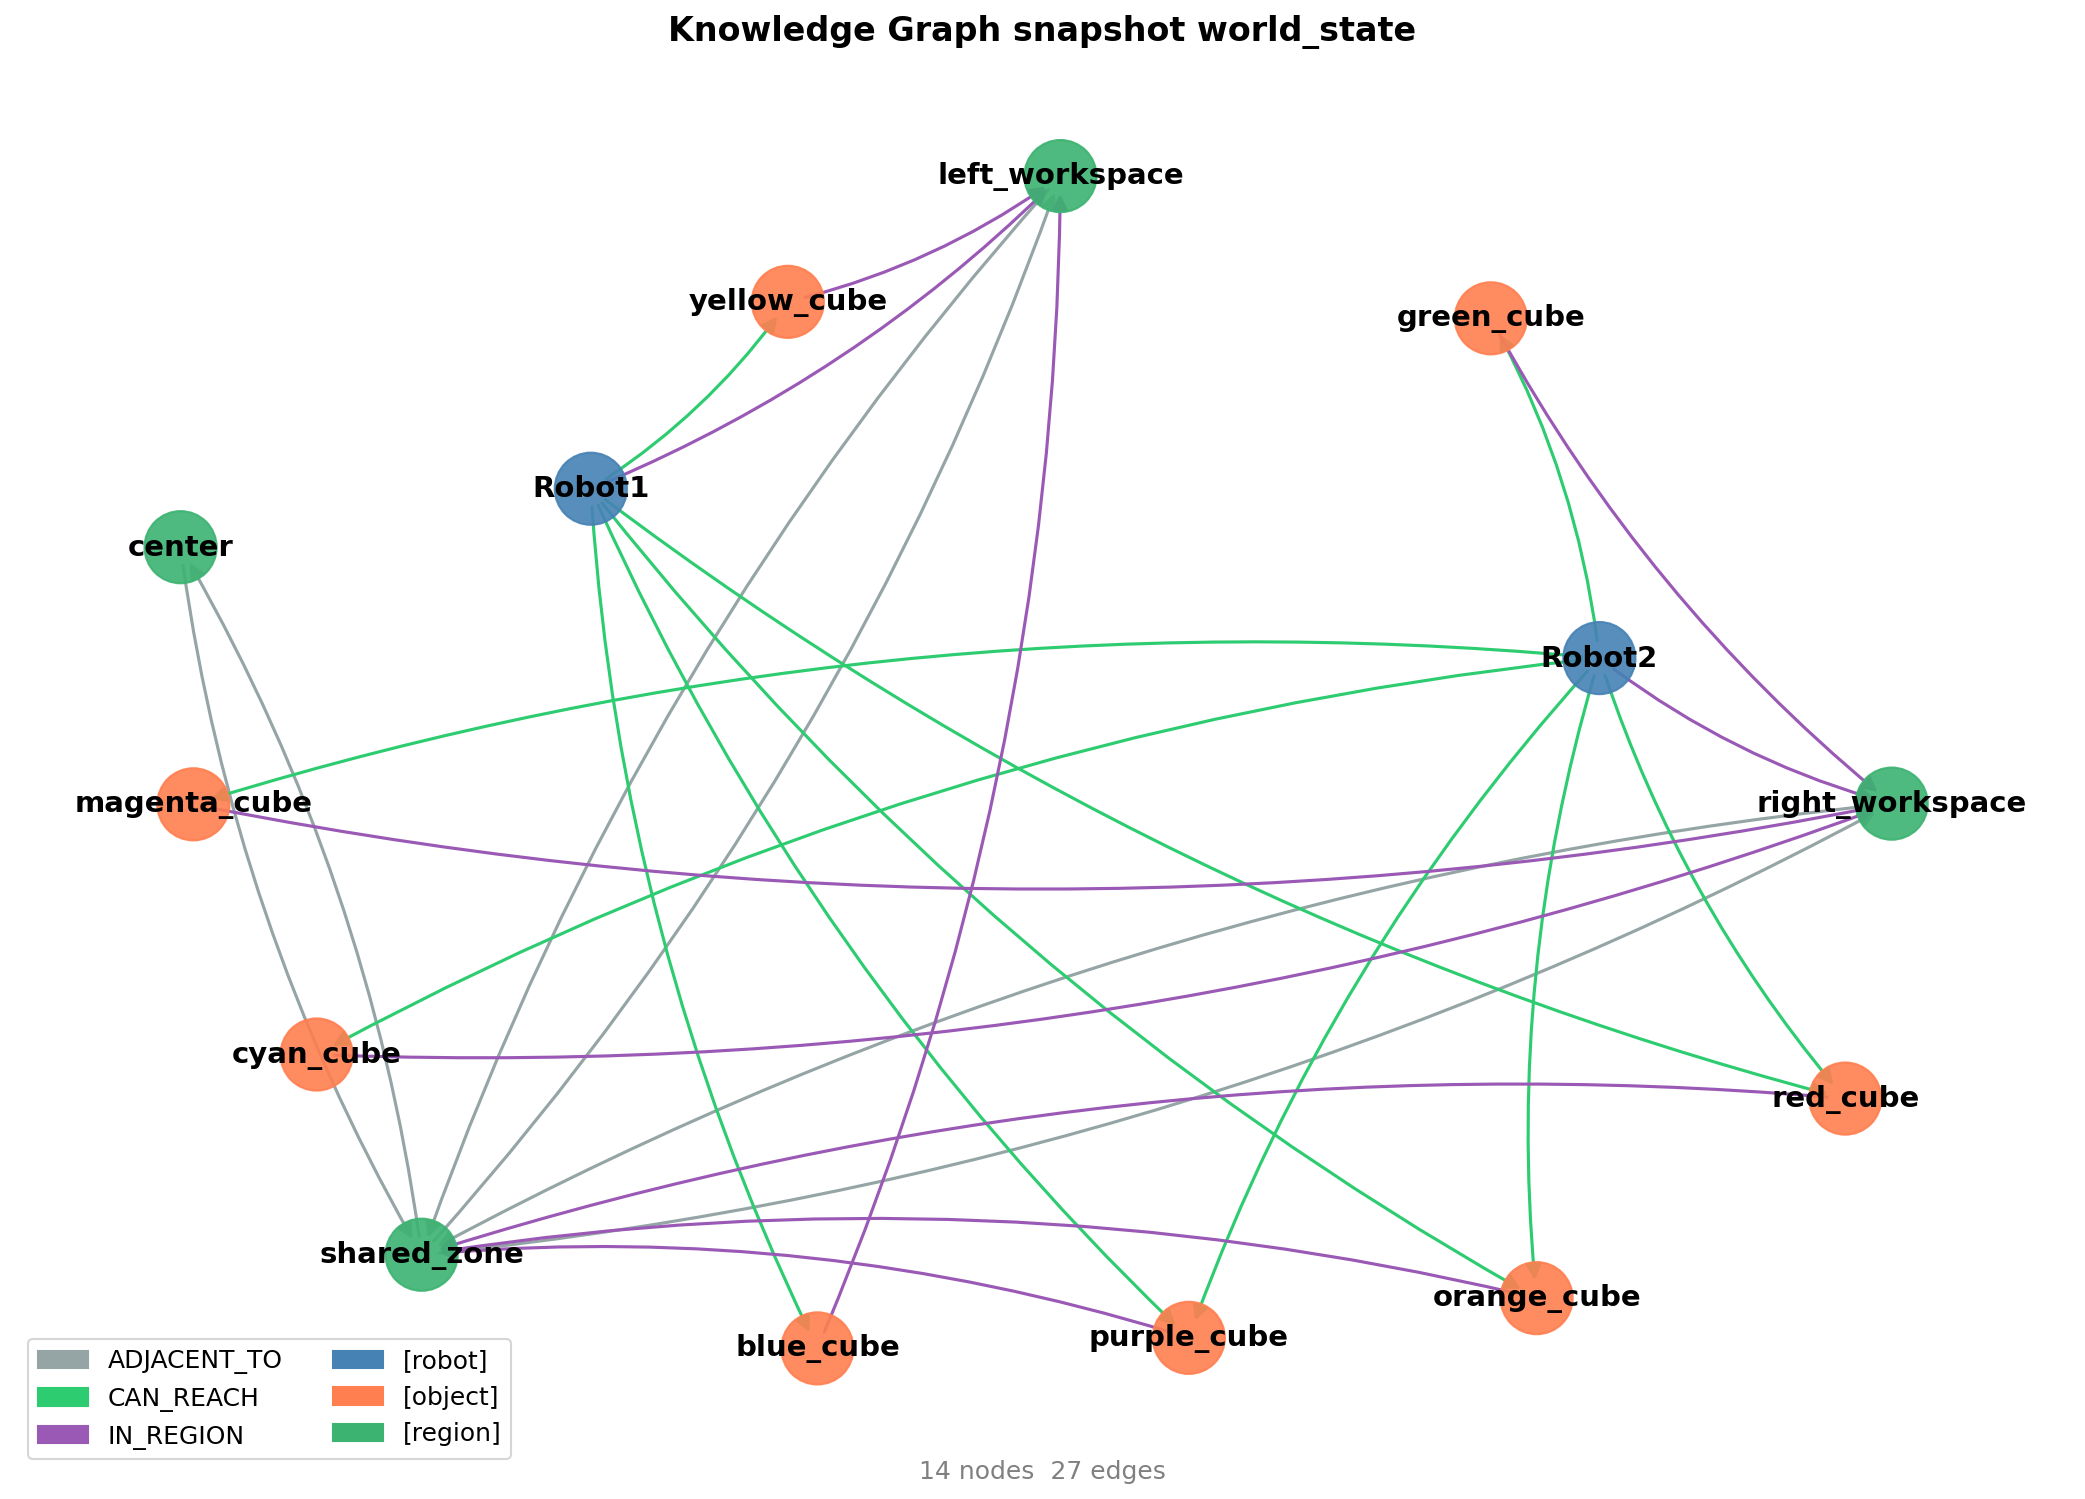
\includegraphics[width=0.75\linewidth]{images/11_kg_world_state.png}
	\caption{The \gls{kg} at simulation start: robot, object, and region nodes with their initial reachability, proximity, and containment edges.}
	\label{fig:kg_example}
\end{figure}

% ------------------------------------------------------------------------------
\section{Benchmark Implementation}\label{sec:benchmark-impl}
Each benchmark is implemented as a self-contained Python module. The single-task benchmarks (B1–B7, B9, B10) expose a \texttt{get\_task()} function that returns one natural-language task; the ablations (B11–B16) expose \texttt{get\_tasks()} returning a list, and B8 exposes \texttt{get\_sub\_tasks()}. The \texttt{BenchmarkRunner} dispatches this string to the live system over the same TCP interface used in normal operation, connecting to the \texttt{SequenceServer}. Most execution benchmarks send the task string through the full parsing pipeline. Two exceptions, B15 (\gls{vgn}) and B16 (\gls{ros}-vs-Unity), dispatch fixed operation chains directly to the sequence executor and bypass the command parser so that grasp quality and movement timing are measured independently of parser variability. For the rest, the command parser translates the natural-language instruction into an ordered list of operations, which the sequence executor then executes in the simulation.

Three benchmarks stop earlier in the pipeline. B9 runs in parse-only mode to evaluate input rejection, and the B11 and B14 ablations evaluate parse quality without dispatching operations to Unity. B17 is the most self-contained of all. It bypasses the \texttt{BenchmarkRunner} dispatch entirely and drives \texttt{RobotConstitution.evaluate\_task()} and the task generator in process, so it runs fully offline with only the local model and no Unity or server stack (Section~\ref{sec:results-autort}).

Results are collected as a \texttt{BenchmarkResult} dataclass that captures step-level metrics, operation name, duration, success flag, and error information, along with aggregate figures: total wall-clock duration, operations executed and succeeded, per-benchmark success rate, mean step duration, and the index of the first failing step. Each run is tagged with a unique identifier that combines a UTC timestamp and a fragment of a universally unique identifier (UUID), enabling each run to be traced. A run is marked successful if and only if the sequence executor reports success for the entire sequence, inheriting the operation-level pass/fail semantics already defined in the system. Benchmark B8 departs from the single-sequence model. Instead of a single fixed task, the runner issues a scripted sequence of 20 heterogeneous natural-language prompts, organized into four phases, repeated over five cycles each, parsed and executed independently, without cross-prompt memory. The chain succeeds only if every sub-task succeeds and every parsed plan fits the expected operation template, making B8 a measure of sustained system reliability.

Between every run, a reset command returns all objects and robots to their initial poses to ensure isolation between trials. A dry-run mode bypasses TCP entirely and executes operations in-process, enabling fast testing of benchmark logic without a running simulation.

Beyond the benchmark framework, both codebases carry automated regression tests so a contributor can confirm a change preserves existing behavior before merging, with roughly 100 subsystem-organized \texttt{pytest} modules on the Python side, many runnable offline via the mock registry and adapter interfaces, and 25 Unity files across EditMode and PlayMode suites driven by the Test Runner.

% ------------------------------------------------------------------------------
\section{Autonomous Task Generation and Coordination}\label{sec:autort-impl}
This section covers the implementation of the system’s autonomous capabilities, how it perceives the scene, generates and filters task candidates, and coordinates activities across two robots. It corresponds to the methods described in Sections~\ref{sec:negotiation} and~\ref{sec:autort}.

\subsection{Vision System}
Object detection uses a fine-tuned \gls{yolo}v8~\cite{yolov8_ultralytics} model trained on a custom cube dataset that covers 17 object classes, including manipulation targets and workspace field markers. The model is loaded at runtime from an Open Neural Network Exchange (ONNX) file, and the actual class count is determined by the model metadata. Images are captured from Unity simulation cameras. Depth estimation uses a stereo camera pair with a 5~cm baseline and a 45$^\circ$ field of view. Stereo disparity is computed using the \gls{sgbm}~\cite{4359315} implementation in OpenCV~\cite{bradski2000opencv} with a tuned preset.

Persistent object tracking between frames uses intersection-over-union matching. Each track maintains a position history for velocity-based prediction. It is aged out after 5 consecutive frames without a match. In multi-robot scenarios, a common vision state module provides a thread-safe object registry with a claim/release mechanism. When one robot claims an object, the other robots see it as unavailable. Stale claims are released after a 10-second timeout, with conflict resolution defaulting to closest-robot priority.

We designed the vision system as an interchangeable component via an abstraction of camera providers. In simulation, a Unity adapter wraps the Unity image store. In real-robot mode, a local adapter connects to cameras instead. No other system component needs to distinguish between the two.

\subsection{AutoRT Implementation}
The AutoRT~\cite{ahn2024autortembodiedfoundationmodels} loop runs only when manually triggered. Each iteration begins with scene capture. Stereo object detection retrieves a complete list of grounded objects with 3D positions. The world state provides robot positions and gripper states, and an optional \gls{vlm} call adds a semantic scene summary. Duplicate objects between stereo detection and the world state are resolved by proximity, so objects within 5~cm of each other are treated as the same object. The resulting scene description is a validated data model, so downstream components can rely on its structure.
Two task candidates are generated in parallel per iteration. The task generation model runs at a temperature of 0.7 to encourage diversity, with up to 3 retries for malformed JSON. On each retry, the parse error is appended to the prompt, giving the model the context it needs to self-correct. Candidates are deduplicated by task identifier before safety filtering. Both layers of the Robot Constitution are then applied. The semantic layer makes a separate \gls{vlm} call at temperature 0, producing near-deterministic decisions. The kinematic layer is pure Python. Workspace bounds are checked against $x \in [-0.4, 0.4]$m, $z \in [-0.4, 0.4]$m, and $y \in [0.0, 0.5]$m. Planned velocities must stay below 2.0 m/s. Gripper force must stay below 50~N. All robot pairs must maintain a separation of at least 0.2~m. These bounds are deliberately tighter than the workspace envelope advertised to the command parser in its prompt (Appendix~\ref{appendix:prompts}) and the \texttt{move\_to\_coordinate} parameter-validation range (Appendix~\ref{appendix:operation_example}), which is wider still in $x$ and $y$ ($z$ is identical), because the autonomous generator must keep self-proposed tasks well inside the reachable region rather than merely within the kinematic limit. A violation in either layer results in the candidate’s rejection.

The balanced task selection strategy scores surviving candidates as

\begin{equation}
	s = 0.6 \cdot r + 0.4 \cdot n,
\end{equation}

where $r$ is the historical success rate for that task type and $n = 1/(1 + \text{attempts})$ is a novelty term that decays with the number of prior attempts. Unseen task types receive a fixed score of 0.7. The selection history is grouped by operation-sequence pattern, so the same conceptual task is recognized regardless of which specific object was involved. Human-in-the-loop approval is enabled by default. It can be disabled with the \texttt{--autonomous} flag.

\subsection{Multi-Robot Negotiation}\label{sec:negotiation-impl}
The negotiation system is activated when the sequence executor detects collaboration keywords or two or more explicit robot identifiers in the input. The negotiation hub is invoked directly as a Python singleton, avoiding the latency and failure modes of an inter-process call.

Each robot is represented by an agent that holds its own conversation context and runs on the same locally hosted model. During analysis, all agents call the \gls{vlm} in parallel. Each returns an assessment of what its robot needs to do and what role it is best suited for. During the proposal, exactly one agent is selected per round in round-robin order. That agent generates a complete sequence of operations covering all participating robots. A plan omitting any robot is rejected, and the remaining agents do not propose in that round. During evaluation, all agents assess the single proposal in parallel and return a binary accept/reject decision, along with a written justification. Both the accept/reject decision and the justifications drive the protocol. When a proposal is rejected, the reviewers' justifications are fed back to the next proposing agent, which must address each one in its revision. Up to three rounds are attempted. If all agents accept, the plan is forwarded to the executor.

A per-agent timeout of 90~s and a global timeout of 300~s bound the worst-case duration. The per-agent timeout applies to each individual call within the protocol; the proposal phase, in which an agent must generate a complete operation sequence, is the most resource-intensive of these calls. Negotiation temperature is set to 0.3, in line with the command parser and well below the 0.7 used for task generation, to allow some variation in proposals while keeping evaluation stable. On any timeout, model error, exhausted rounds without consensus, or other failure, the system silently falls back to the standard single-model command parser.
%%%%%%%%%%%%%%%%%%%%%%%%%%%%%%%%%%%%%%%%%%%%%%%%%%%%%%%%%%%%%%%%%%%%%%%%%%%%%%%%
%%  BENCHMARKS AND EVALUATION
%%%%%%%%%%%%%%%%%%%%%%%%%%%%%%%%%%%%%%%%%%%%%%%%%%%%%%%%%%%%%%%%%%%%%%%%%%%%%%%%
\chapter{Benchmarks and Evaluation}\label{evaluation}
This chapter defines the benchmarks we use to test the system and explains the criteria we use to select and organize them. The benchmarks progress from basic single-robot operations to collaborative multi-robot tasks, culminating in sustained autonomous operation. Additionally, we use ablation analyses to isolate the contributions of individual architectural components.

% ------------------------------------------------------------------------------
\section{Benchmark Framework}\label{sec:benchmark-framework}
Seventeen benchmarks evaluate system capabilities across the full operational range, grouped into four tiers: a single-robot baseline increasing from object-directed navigation to pose-aware grasping (B1--B5), dual-robot collaboration (B6--B7), system-robustness probes (B8--B10), and single-flag ablations (B11--B16), followed by the offline AutoRT~\cite{ahn2024autortembodiedfoundationmodels} evaluation (B17). The ablations isolate the impact of \gls{rag}~\cite{lewis2021retrievalaugmentedgenerationknowledgeintensivenlp}-augmented parsing, reflection recovery, negotiation, \gls{kg}~\cite{Hogan_2021} context, \gls{vgn}~\cite{breyer2021volumetricgraspingnetworkrealtime} versus geometric fallback, and \gls{ros}~\cite{Macenski_2022}/MoveIt~\cite{coleman2014reducingbarrierentrycomplex} path computation versus direct Unity control, while B17 exercises the AutoRT task generator and two-layer safety gate offline. The full per-benchmark list is in Appendix~\ref{appendix:benchmarks}.

Each ablation benchmark uses its own purpose-built task set and is run under both conditions, a single feature flag enabled or disabled, so the same strings are compared flag-on versus flag-off to isolate the component's effect. The benchmark harness itself (module structure, task dispatch, the parse-only and fixed-chain modes, and the inter-run \texttt{reset\_simulation}) is described in Section~\ref{sec:benchmark-impl}.

% ------------------------------------------------------------------------------
\section{Evaluation Metrics}\label{sec:evaluation-metrics}
We collect results at two levels of granularity. At the step level, each operation records success or failure, wall-clock duration, and a structured error code when it fails. At the task level, we mark a run successful when the sequence executor reports overall success for the dispatched task. We derive several metrics from these records and visualize them in the web dashboard’s analysis tab. Together, they answer three questions: whether the system works, whether each architectural component contributes, and whether performance is sufficiently consistent to be credible.

\subsection{Primary metrics}
\begin{description}
	\item[Success rate] is the central metric and direct evidence for the thesis claim that the system reliably executes \gls{vlm}-generated plans among tasks of increasing complexity. A run is marked successful when the sequence executor reports overall success for the task. Several benchmarks add a stricter check, conjoined with that flag: those with a defined reference plan also require the parsed operation sequence to match it exactly, B10 additionally requires a parallelism ratio of $\geq 0.5$, and B9 inverts the criterion, counting a run as successful only when the parser correctly rejects the task. Where tables report an operation-level success rate for a multi-run condition, it is the pooled count of successful operations over operations executed across that condition’s runs.
	\item[Task duration] reports wall-clock time per benchmark. It also serves as a sanity check, as a benchmark with high success and suspiciously low duration may indicate trivial execution. Reported durations cover operation execution only; the initial model parse preceding execution is not included, but reflection re-parses triggered during execution fall inside the measured window and are therefore part of the total.
	\item[Multi-run stability] reports mean and \gls{sd} across repeated runs. \gls{vlm}-based systems are non-deterministic by nature, so a single run proves nothing. High variance at a given benchmark level indicates unreliability, even when the mean success rate looks acceptable.
\end{description}

\subsection{Large Language Model command parse accuracy}
In benchmarks B1–B8 and B10, the model parses each natural-language task string into an operation sequence, which is then executed. Because of this, plan correctness is reflected in the run’s success rate rather than being scored separately. To directly isolate and evaluate parse quality, ablations B11 and B14 inspect the parsed plans without dispatching them. Each ablation pairs the system against a flag-disabled baseline to determine causal impact.

B14 isolates whether \gls{kg} context helps the model reference correct object labels instead of hallucinating plausible-sounding ones. It applies two structural checks, which are reported together as a single bad-operation rate. Parse accuracy flags parsed operations whose names resolve to no registered entry in the operation registry as hallucinated. Object-reference correctness is checked structurally. A parameter qualifies as a valid reference if it uses a \texttt{\$}-prefixed variable or names a known object, and a \gls{kg}-aware operation that references neither is flagged as a wrong-object reference, indicating the model invented a label.

Similarly, B11 isolates how \gls{rag} retrieval affects an additional metric, operation-selection accuracy, defined as the fraction of tasks whose parsed plan contains the single ground-truth operation the task is designed to elicit, checked anywhere in the plan since a name- or color-referenced task legitimately decomposes into a detect-then-act sequence. Each B11 task is deliberately ambiguous, with several registered operations that could plausibly satisfy the description but only one correct given the system’s semantics, so the metric measures whether retrieval steers the parser to the intended operation.

\subsection{Grasp metrics}
Grasp success rate is measured as the fraction of grasp attempts in which the object is actually held and lifted clear of the table. We also report execution time per operation, grouped by the functional categories from Figure~\ref{fig:operation_map}. The manipulation operations dominate, with \texttt{grasp\_object} averaging over 15~s per grasp across the benchmark suite. B15 compares the \gls{vgn} grasp path against the geometric top-down baseline, using the same held-and-lifted criterion.

\subsection{Multi-robot synchronization}
Dual-robot benchmarks B6 and B7 coordinate two arms by explicit \texttt{signal} and \texttt{wait\_for\_signal} primitives. Barrier latency, the time the receiving robot spends blocked, from when it begins waiting to when the expected signal unblocks it, is captured as the duration of the \texttt{wait\_for\_signal} step on that robot. The coordination failure mode tracked is \texttt{WAIT\_TIMEOUT}, raised when a robot waits beyond the configured timeout without receiving the expected signal.

Negotiation ablation B13 records the number of negotiation rounds completed, using rounds from the hub and, if that fails, the signal-op count in the parsed plan as a proxy for coordination effort. Additionally, a per-robot step breakdown reports the total step time for each arm in the dual-robot benchmarks; a balanced distribution indicates coherent coordination, with neither arm left idling.

\subsection{Diagnostic metrics}
The web dashboard’s analysis tab provides several diagnostic visualizations to support debugging and interpretation of results. The operation timing heatmap cross-references benchmarks with individual operations, with cells colored by the average duration per operation, allowing us to spot context-dependent slowdowns, such as \texttt{grasp\_object} taking longer in B7 than in B4 due to multi-robot workspace contention. Complexity scaling plots plan length against total execution time; roughly steady scaling indicates the system does not degrade as plans grow longer, while superlinear scaling would flag an architectural bottleneck. B8 is excluded from this chart because its plan is assembled from sub-tasks and not parsed from a single command.

We reproduce the operation reliability heatmap diagnostic view here as Figure~\ref{fig:reliability_heatmap}. It reports per-operation success rates across the benchmarks, pooled over runs and models. It also doubles as a coverage check, because the populated cells confirm that the suite exercises a representative subset of the operation registry, with a clear progression of capabilities from B1 to the multi-step collaborative benchmarks, while the cell colors expose where individual operations become unreliable in specific situations.

\begin{figure}
	\centering
	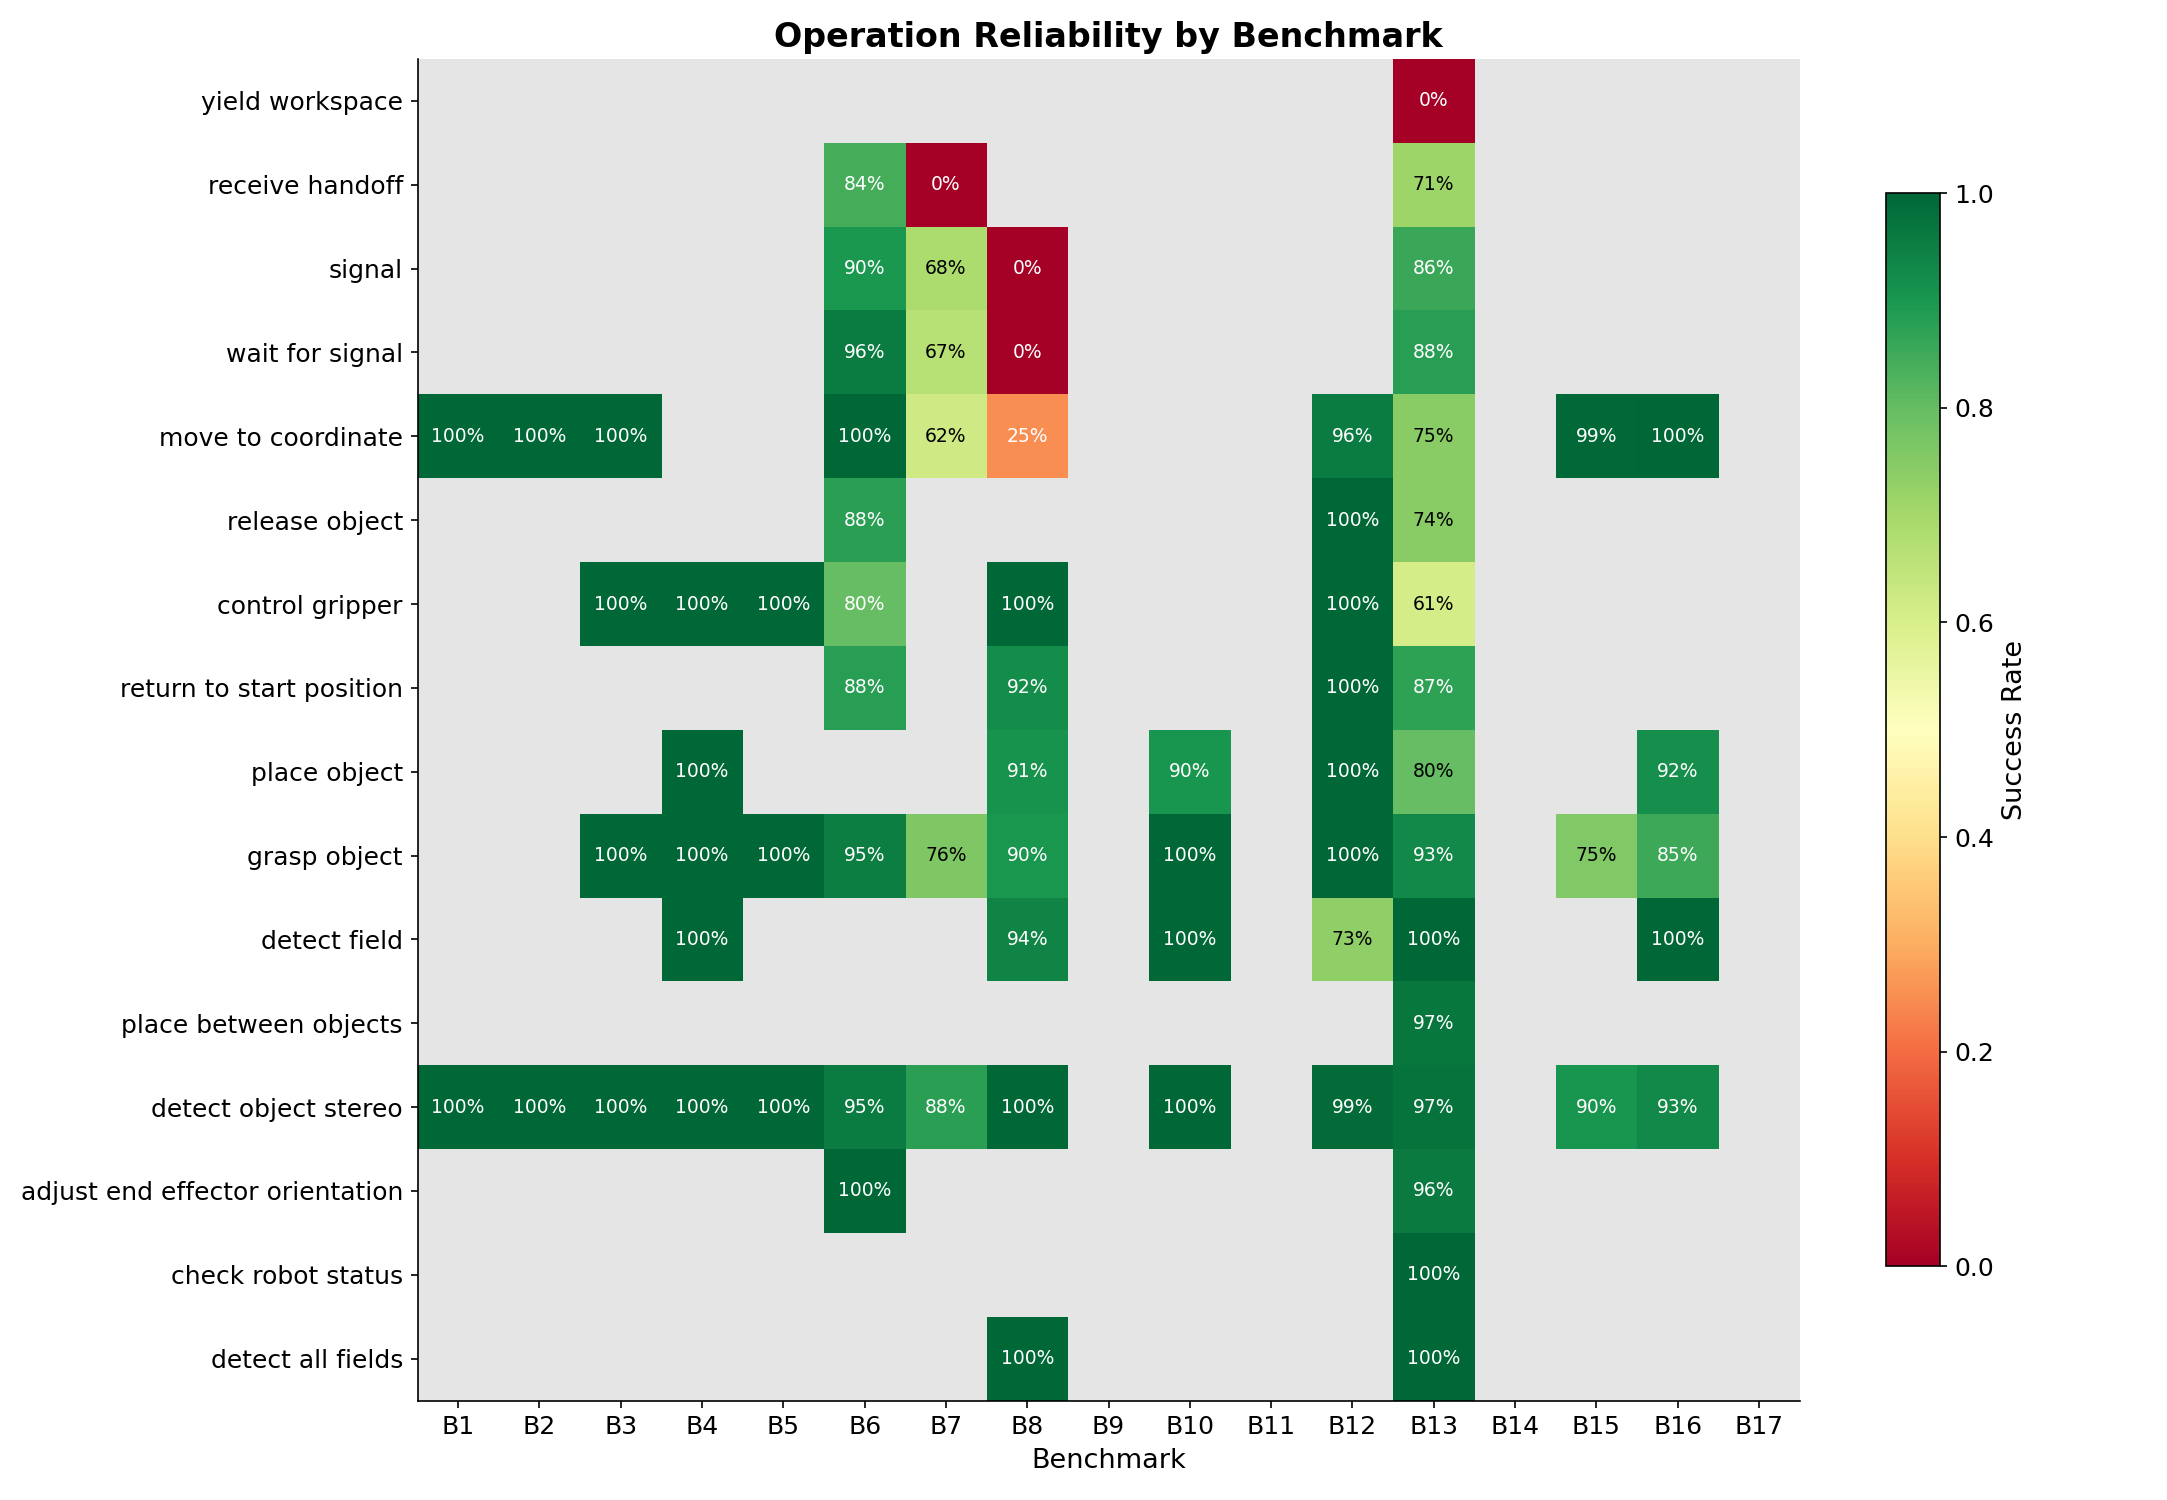
\includegraphics[width=1\linewidth]{images/06_reliability_heatmap.png}
	\caption{Operation reliability by benchmark: aggregated per-operation success rates across all models. Gray cells indicate that the operation does not occur in that benchmark. The synchronization operations are reliable in well-formed plans, degrade in B7, and collapse in B8, where they appear only in non-conforming plans from weaker backends, so every occurrence necessarily times out with no partner listening.}
	\label{fig:reliability_heatmap}
\end{figure}

% ------------------------------------------------------------------------------
\section{Results}\label{sec:results}
We ran all benchmarks on an Apple MacBook Pro with an M5 Pro Chip with 64~GB of unified memory, running the Unity~\cite{unity} 6000.3.11f1 simulation, the Python backend, and a Docker-hosted \gls{ros}/MoveIt stack on the same machine. \gls{magi}~\cite{mistral_magistral_small_2025}, served locally through LM Studio~\cite{lmstudio}, was the default \gls{vlm} backend unless stated otherwise. We ran each benchmark five times consecutively, resetting the simulation between runs; the B9, B11, B12, and B13 sweeps and the \gls{magi} B16 comparison were subsequently extended to twenty runs per condition to tighten those estimates. Unless noted, we kept all feature flags active throughout. The \gls{kg} stays at its enabled default rather than being toggled per run. B14 shows it carries a small parse-quality cost, but that cost sits within run-to-run noise, and the \gls{kg} only supplies additive spatial context to detection and handoff reasoning that fails safe when it is absent, so nothing in the execution or safety path depends on it. The negotiation protocol, in contrast, is disabled in all system runs. Beyond keeping cross-run and cross-model comparisons clean by isolating a single variable, this reflects what negotiation is for. It resolves role-assignment ambiguity, and only B13’s tasks present that ambiguity by design. The other multi-robot benchmarks explicitly specify roles. B6, for instance, names both the initiating and the receiving arm, so negotiation would introduce no ambiguity there and would add multi-agent latency and variance without changing the plan.

This section reports results across the four benchmark tiers introduced in Section~\ref{sec:benchmark-framework}, followed by the offline AutoRT evaluation. Detailed per-run metrics are in Appendix~\ref{appendix:benchmark_runs}.

Figure~\ref{fig:success_by_model} summarizes success rates per benchmark for the six models evaluated across the full suite, and Figure~\ref{fig:model_task_heatmap} condenses the same data into a model–task matrix. A few patterns are visible before any individual benchmark is examined. All models solve the simplest navigation tasks, but the single-robot tier already separates them from B3 onward. \gls{magi}, \gls{mini}, \gls{gema42}, and \gls{gema44} all clear the single-robot tier at full task success, while the Qwen3-VL family is the weak performer here. \gls{qwen38} fails B3, and \gls{qwen330} is unreliable across B3–B5, not by mis-executing the grasp, but by emitting truncated plans that omit the grasp-and-place steps, which execute without error yet do not accomplish the task. B6 separates the models sharply. Only \gls{magi} and \gls{mini} complete the handoff in every run, with \gls{gema44} succeeding in three of five, while B7 defeats all six. B9 inverts the usual ordering. Only \gls{gema42} refuses the impossible task with any consistency, and it does so by emitting no plan at all, while every stronger planner generates commands for it. The per-benchmark sections below unpack each result.

\begin{figure}
	\centering
	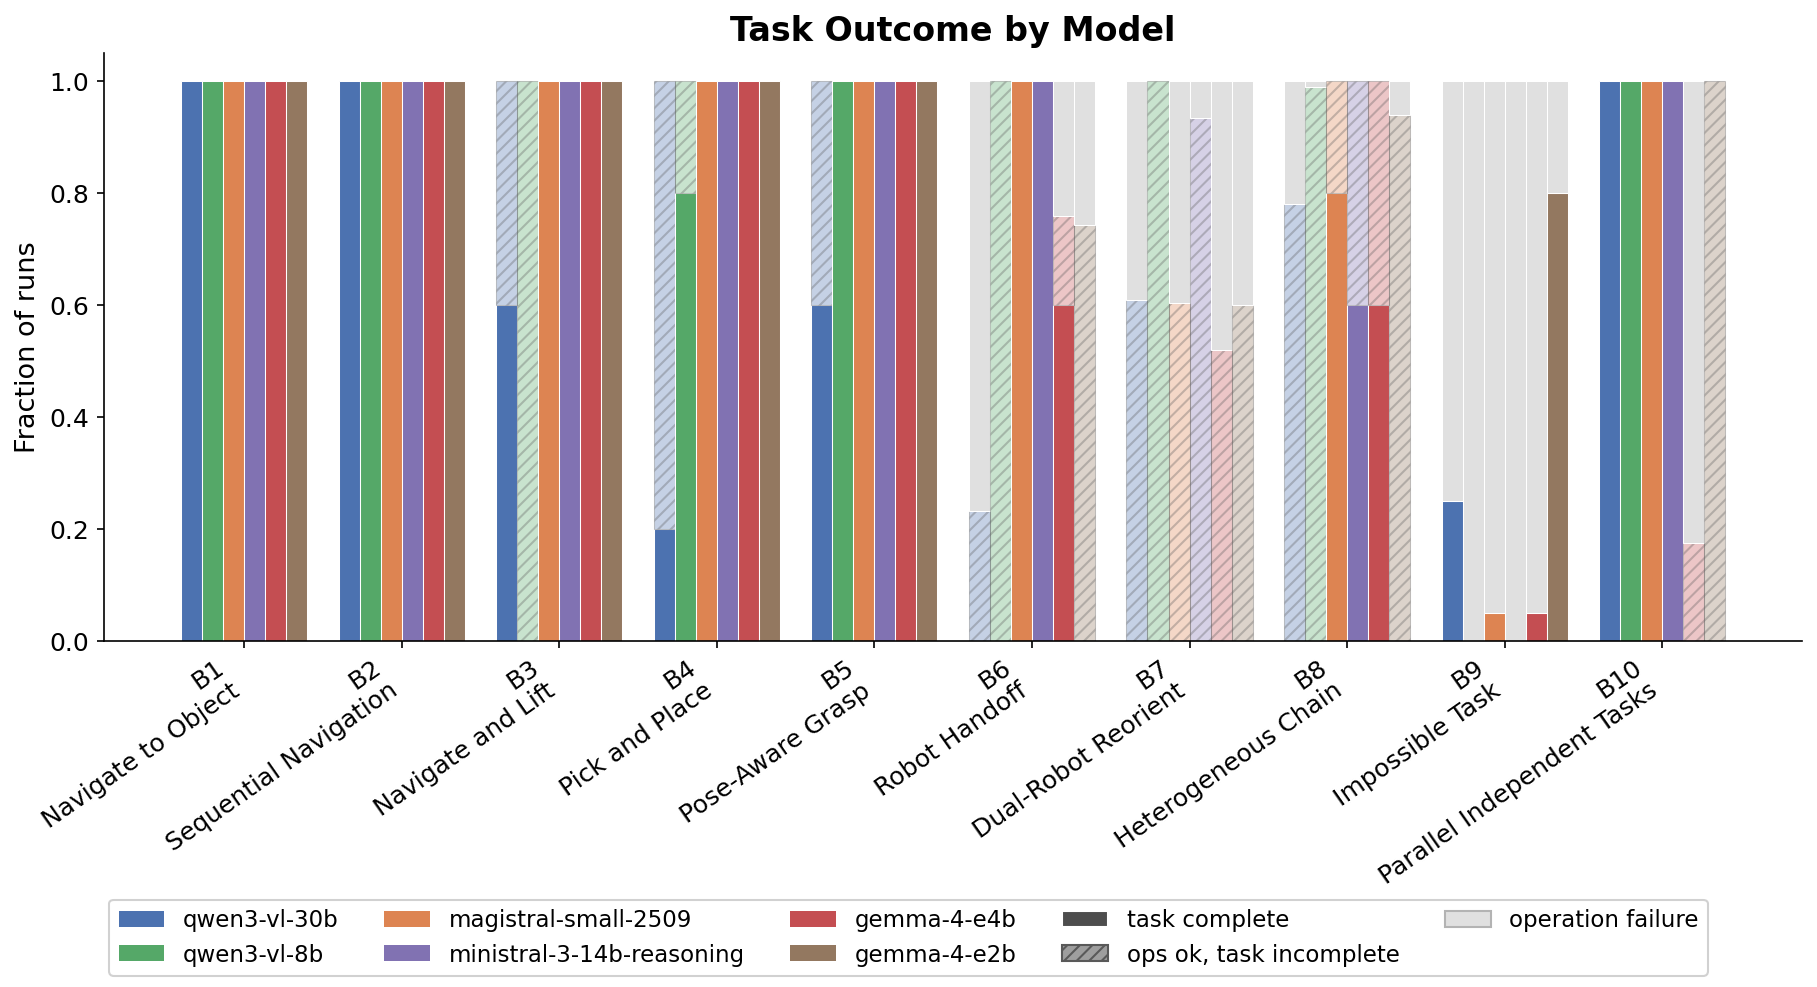
\includegraphics[width=1\linewidth]{images/01_success_rate_by_model.png}
	\caption{Task outcome per benchmark and model. Each bar is a full-height stack. The solid lower segment is the fraction of runs that complete the task, the hatched middle segment is runs whose emitted operations succeed but whose plan is too short to finish the task, e.g.\ \gls{qwen38} reducing B3 to a single detection, and the light upper segment is operation failures.}
	\label{fig:success_by_model}
\end{figure}

\begin{figure}
	\centering
	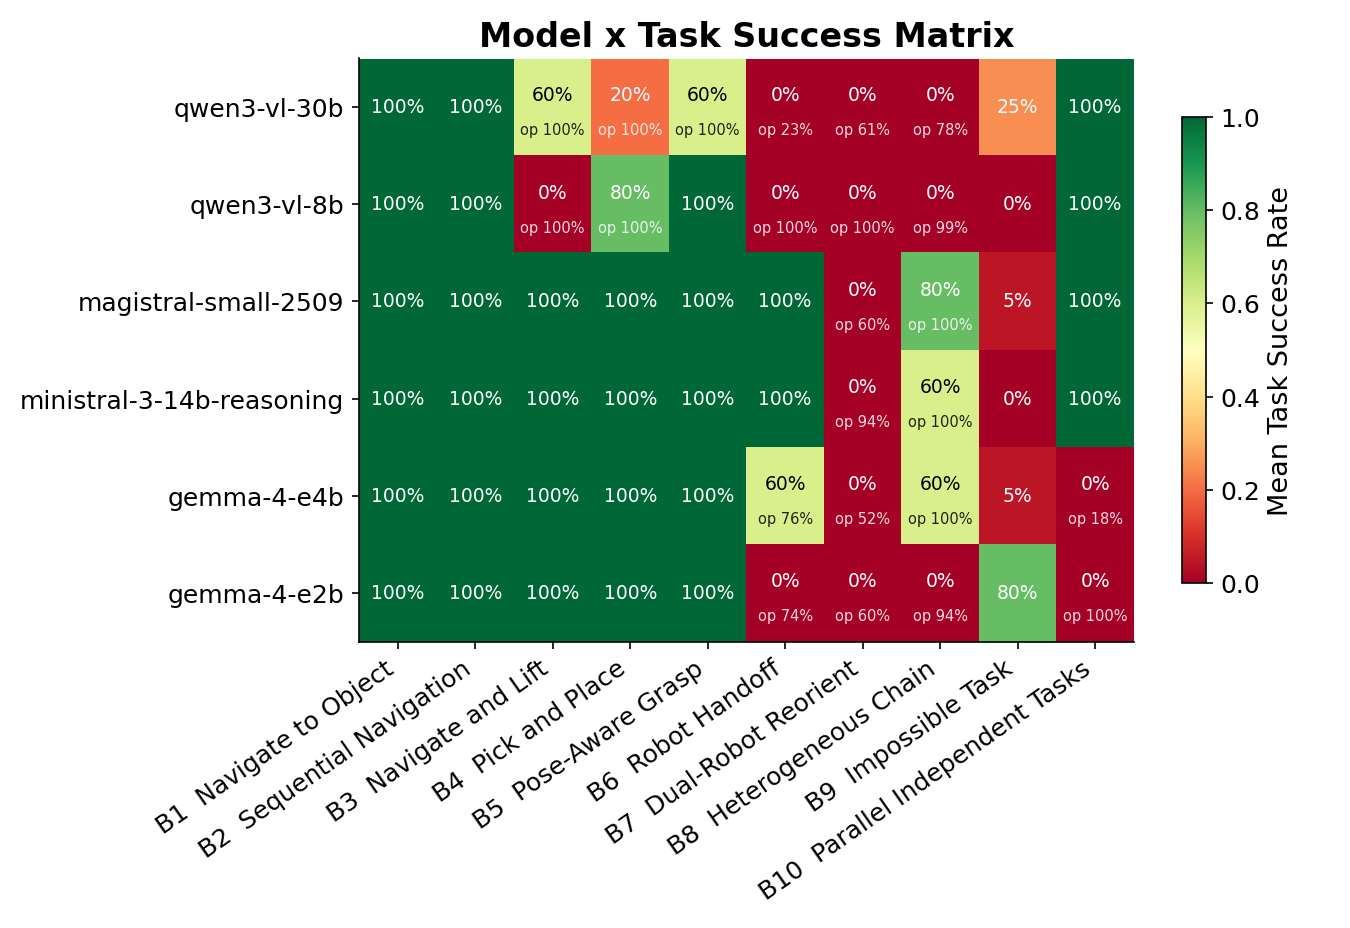
\includegraphics[width=1\linewidth]{images/02_model_task_heatmap.png}
	\caption{Model–task success matrix across all models (mean task success rate over five runs, twenty for B9; the small op subscript gives the operation-level rate where it diverges from task completion). The B9 column shows the inverted capability ordering discussed in Section~\ref{sec:results}: at twenty runs per model, only \gls{gema42} rejects the impossible task with any consistency (0.80), while every stronger planner emits commands for it.}
	\label{fig:model_task_heatmap}
\end{figure}

\subsection{Single-Robot Tasks}
Five benchmarks evaluate individual-robot performance along a complexity gradient. B1 navigates to a stereo-detected object; B2 chains two such navigations; B3 adds a grasp and transport; B4 runs the full detect–grasp–detect-field–place pipeline; and B5 exercises the grasp-planning path with a pose-aware grasp that requires detection but no transport. We report the tier in detail for \gls{magi}, whose behavior the other three clearing models reproduce. Across its 25 runs, the system achieved a task completion rate of 1.000 with no hallucinated operations and no retries, producing the same operation sequence across all 5 runs of each benchmark.

Two behaviors break the otherwise uniform timing. In B4, the grasp completes faster than in B3 because the object is consistently presented in an accessible pose, allowing the planner to converge quickly. Object-pose predictability, not plan structure, is the primary driver of grasp cost. In B5, the grasp is marginally faster than B3’s in absolute terms, the target being easier to reach, but more variable (\gls{cv} $=\sigma/\mu$ of 0.36 versus 0.28).

Table~\ref{tab:single-robot-latency} pools latencies for the highest-cost primitives; Figure~\ref{fig:op_latency} extends the view across the suite as per-operation box plots. Stereo detection is the most stable primitive (\gls{cv}~9\% across 30 pooled steps). Navigation variance (\gls{cv}~30\%) reflects dependence on inter-pose distance. End-to-end duration scales with the cost of physical manipulation rather than plan length alone. B2 takes four steps, 10.01~s, and is faster than B5’s two steps, including a pose-aware grasp, which takes 20.00~s. These results establish a strong individual-robot baseline and motivate the dual-robot benchmarks, in which correct coordination must be achieved on top of this foundation.

\begin{table}[t]
	\centering
	\resizebox{\textwidth}{!}{
		\begin{tabular}{llcccc}
			\hline
			\textbf{Operation}              & \textbf{Benchmarks}   & \textbf{n}         &
			\textbf{Mean (s)}               & \textbf{\gls{sd} (s)} & \textbf{Range (s)}                               \\
			\hline
			\texttt{detect\_object\_stereo} & B1–B5                 & 30                 & 0.80  & 0.07  & 0.74–0.94   \\
			\texttt{move\_to\_coordinate}   & B1–B3                 & 20                 & 4.37  & 1.32  & 3.06–7.18   \\
			\texttt{grasp\_object} (B3)     & B3                    & 5                  & 19.84 & 5.52  & 16.00–29.55 \\
			\texttt{grasp\_object} (B4)     & B4                    & 5                  & 10.93 & 1.37  & 8.94–12.56  \\
			\texttt{grasp\_object} (B5)     & B5                    & 5                  & 17.70 & 6.39  & 10.53–23.43 \\
			\texttt{place\_object}          & B4                    & 5                  & 34.43 & 11.52 & 23.42–51.42 \\
			\hline
		\end{tabular}
	}
	\caption{Pooled operation latencies across single-robot benchmarks.}
	\label{tab:single-robot-latency}
\end{table}

\begin{figure}
	\centering
	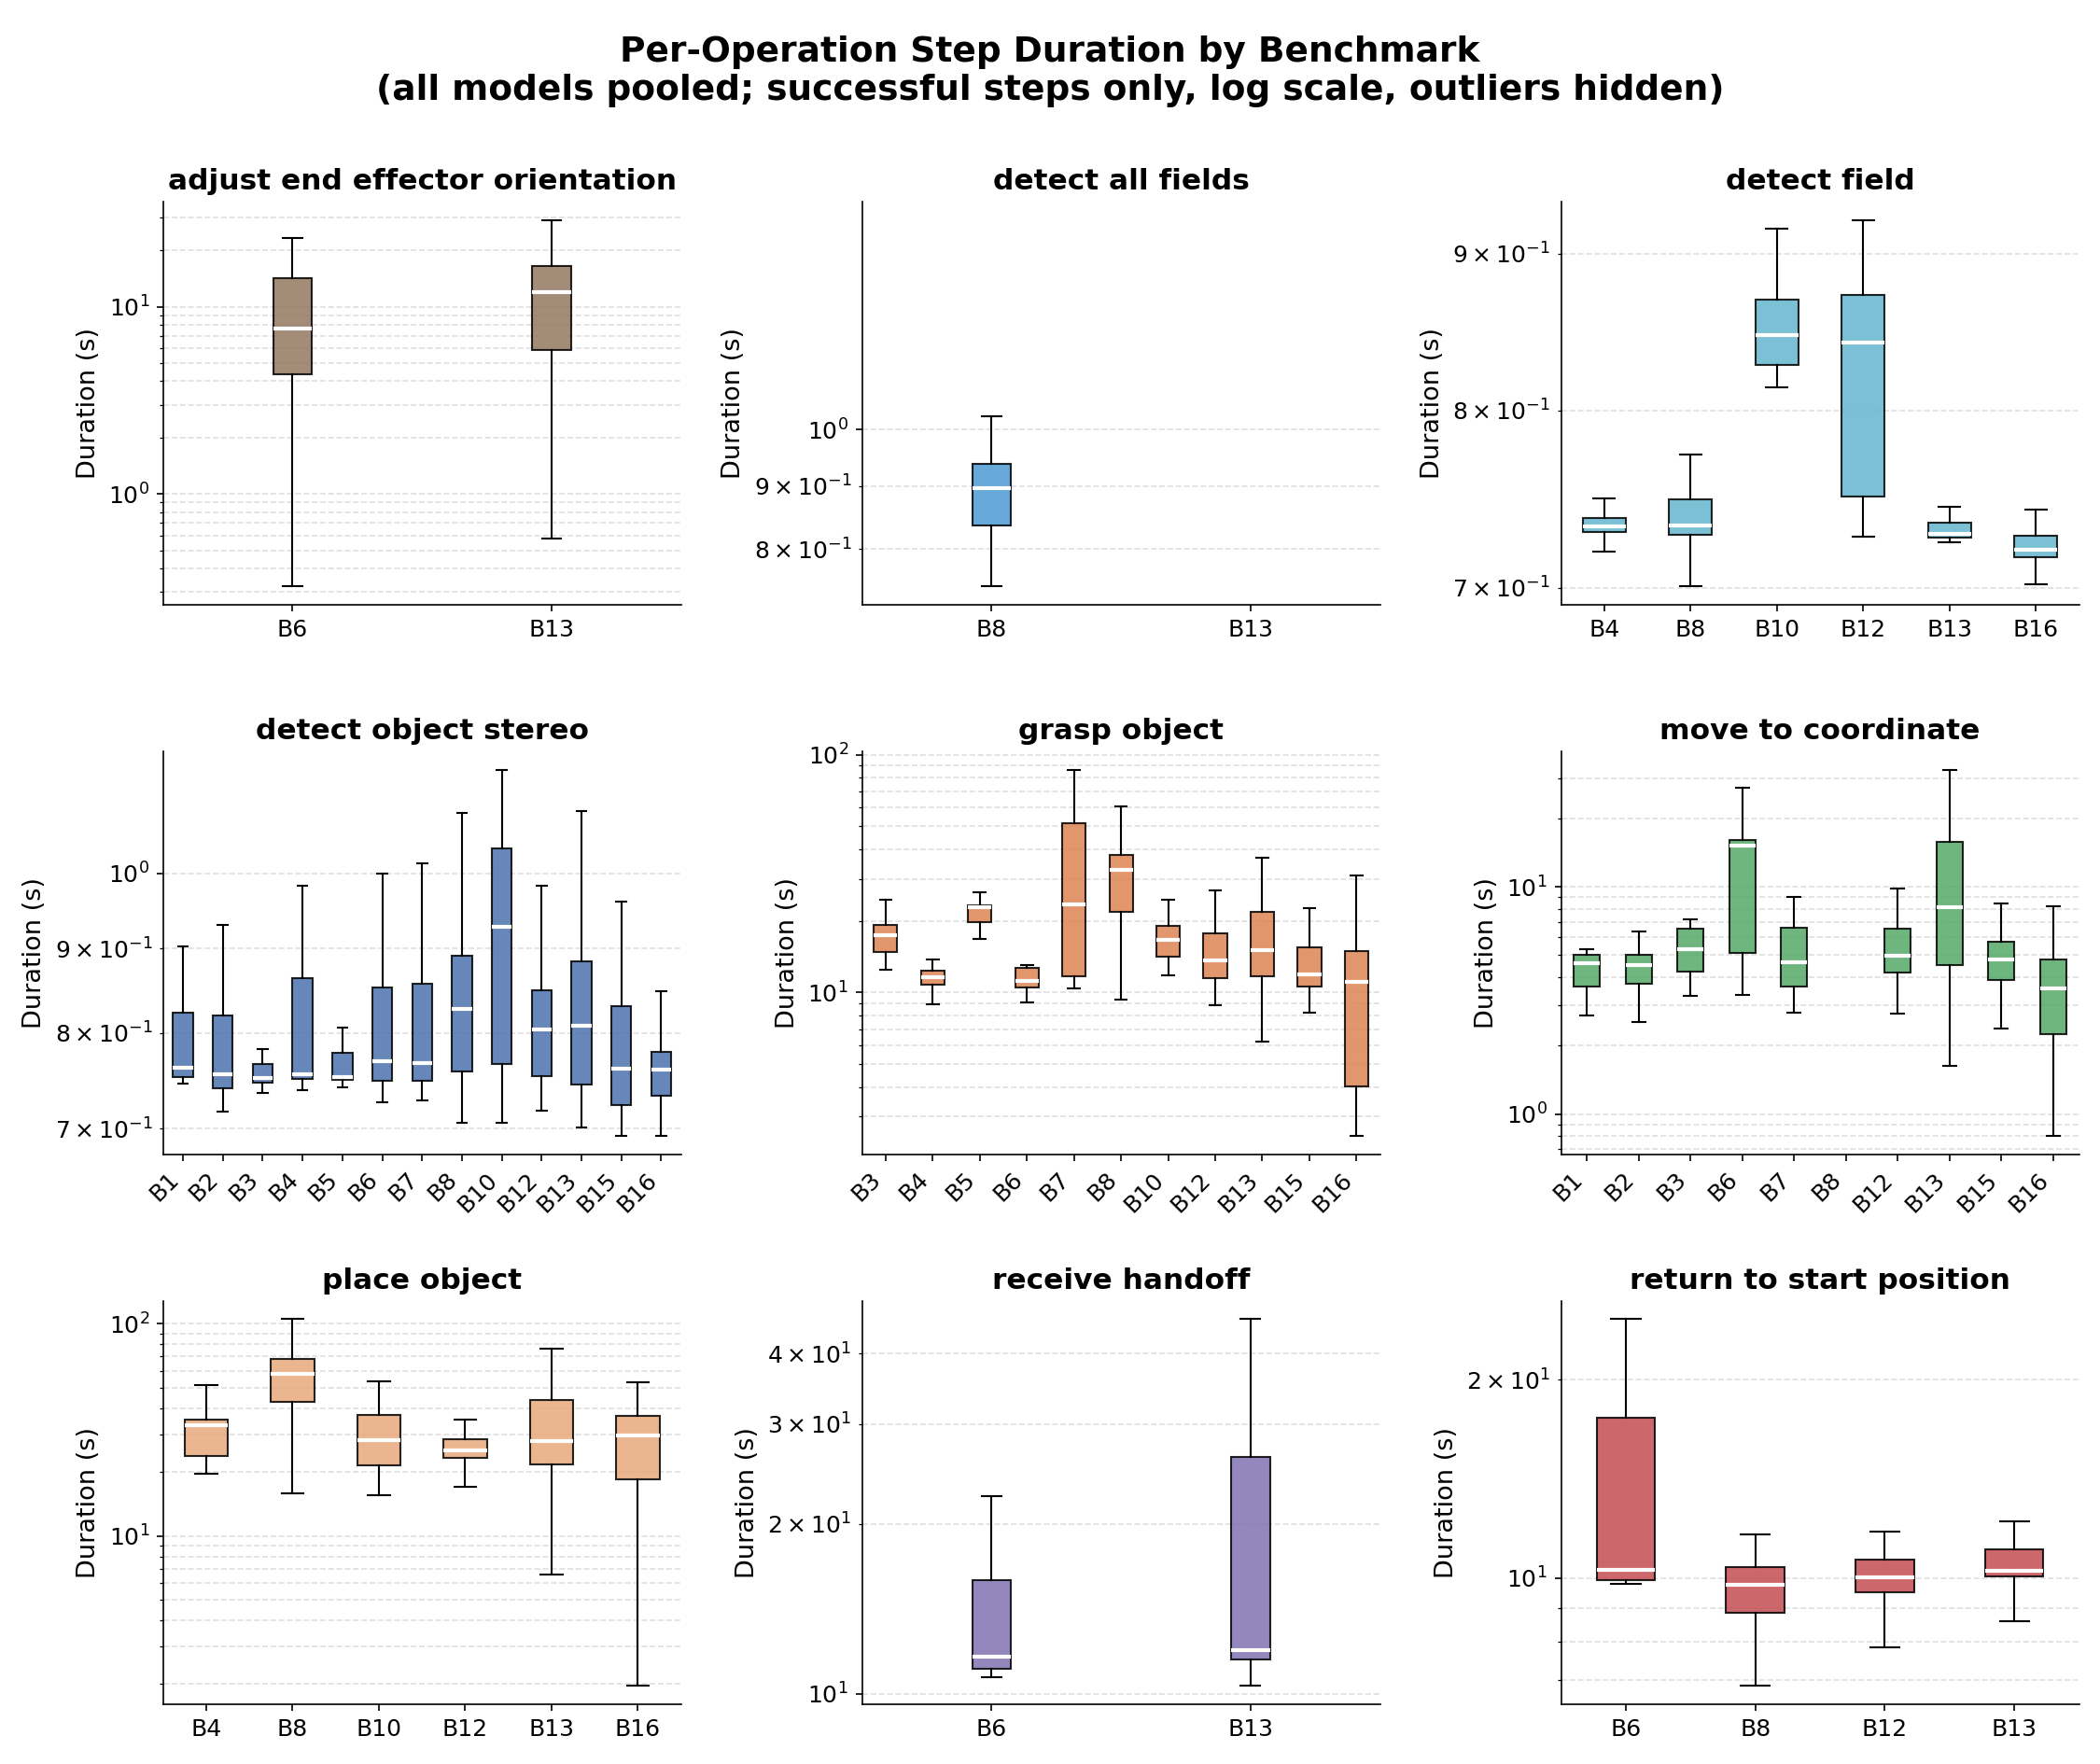
\includegraphics[width=1\linewidth]{images/05_op_latency.png}
	\caption{Aggregated per-operation step durations by benchmark. Perception primitives \texttt{detect\_field} and \texttt{detect\_object\_stereo} cluster tightly below one second, while the contact-rich primitives like \texttt{grasp\_object} and \texttt{place\_object} dominate total task time and carry the widest spread.}
	\label{fig:op_latency}
\end{figure}

\subsection{Dual-Robot Tasks}\label{sec:results-dual}
Two benchmarks evaluate the system’s ability to coordinate actions across both arms. B6 tests sequential handoff coordination, in which robots act in turn at an explicit synchronization point. B7 escalates this to concurrent physical coupling, in which both robots must grasp a shared object simultaneously. Together, they define the current boundary of coordination capability.

\subsubsection{B6 — Robot Handoff}
The task prompt is \textit{Robot1 grasps the red cube and hands it to Robot2}. The system must plan and execute a multi-step, two-robot sequence covering perception, grasping, spatial repositioning, synchronization, and handoff reception without explicitly listing these sub-steps in the prompt.

Two models, \gls{magi} and \gls{mini}, produced complete handoff plans and achieved a task success rate of 1.000; \gls{gema44} succeeded in three of five runs. The remaining three failed at different stages of plan construction. \gls{qwen38} generated a single-operation plan in all five runs, never proceeding to grasp or transfer. \gls{qwen330} produced an empty plan in three of five runs and partial executions in the other two, only one of which contained a complete handoff chain. \gls{gema42} produced an empty plan in one run and longer, non-conforming plans in the other four, usually executing every operation but deviating from the expected handoff chain without ever scoring a completed handoff. We report the successful pattern in detail for \gls{magi}. Four \gls{magi} runs produced an identical nine-operation plan; one run appended an additional \texttt{return\_to\_start\_position} and \texttt{signal} at the end:

\begin{lstlisting}
detect_object_stereo -> grasp_object -> move_to_coordinate -> adjust_end_effector_orientation -> signal || wait_for_signal -> detect_object_stereo -> receive_handoff -> release_object
\end{lstlisting}

All 47 operations across the five runs executed successfully on the first attempt. Mean total duration was 58.3~s (\gls{sd} = 16.2~s), ranging from 43.3~s to 82.8~s across runs. Three contact-rich primitives, \texttt{move\_to\_coordinate}, \texttt{grasp\_object}, and \texttt{receive\_handoff}, dominate, together accounting for roughly 59\% of total task time (Table~\ref{tab:b6-latency}), while the synchronization constructs completed in under 1~ms in every run, consistent with their role as logical barriers. The per-operation means sum to $\sim$42~s, but the residual is not a steady per-step tax. Three of the five runs match their own step-duration sum to within 1.5~s, while the two longest runs carry residuals of 35.4~s and 31.6~s, respectively; these residuals arise during execution, between the per-step measurements.

\begin{table}[t]
	\centering
	\begin{tabular}{lcc}
		\hline
		\textbf{Operation}                           & \textbf{Mean (ms)} & \textbf{\gls{sd} (ms)} \\
		\hline
		\texttt{detect\_object\_stereo}              & 878                & 119                    \\
		\texttt{grasp\_object}                       & 11{,}286           & 1{,}556                \\
		\texttt{move\_to\_coordinate}                & 12{,}077           & 4{,}975                \\
		\texttt{adjust\_end\_effector\_orientation}  & 6{,}079            & 1{,}934                \\
		\texttt{signal} / \texttt{wait\_for\_signal} & $<$1               & –                      \\
		\texttt{receive\_handoff}                    & 11{,}152           & 379                    \\
		\texttt{release\_object}                     & 2                  & 1                      \\
		\hline
	\end{tabular}
	\caption{B6 per-operation mean latencies averaged across five runs (\gls{magi}).}
	\label{tab:b6-latency}
\end{table}

The high variance in \texttt{move\_to\_coordinate} reflects variation in the handoff position across runs. The step alone takes 6.4~s to 15.7~s depending on the chosen coordinate, which drives the elevated variance in total duration. The success rate is only part of what B6 shows; the rest is how the coordination arose. The system identified the need for a synchronization barrier at the handoff, so that Robot~2 begins its receiving motion only after Robot~1 signals readiness through the signal/wait primitives. The plan correctly realizes the handoff’s temporal dependency. The instruction never lists this ordering; the system prompt’s handoff rule does, so these runs show reliable rule-following for the constraints the chain matcher enforces: orientation before signaling, reception before release. The rule’s two \texttt{return\_to\_start\_position} steps, by contrast, are prescribed in the same ordering-constraint block yet are systematically ignored. Four of the five plans omit both, and the remaining run instead appends a single \texttt{return\_to\_start\_position} plus a trailing \texttt{signal} at the end of the plan. The chain matcher treats the returns as optional, so scoring is unaffected, but the pattern indicates the model weights positional constraints more heavily than clear-the-workspace steps.

During development, we observed that the model could sometimes compose the correct \texttt{signal}$\rightarrow$\texttt{wait\_for\_signal}$\rightarrow$\texttt{receive\_handoff} ordering from the task description alone, with no handoff-specific guidance. This was not consistent across models or runs. Some backends emitted a flat command list, while others dropped the synchronization barrier entirely. We therefore added an explicit handoff rule to the prompt and a reusable coordination pattern to the retrieval layer, thereby making ordering reliable and consistently reproducing concurrent co-grouping. The benchmark runs use this default configuration, so they demonstrate dependable rule-following built on a capability the model also shows, more weakly, on its own.

\subsubsection{B7 — Dual-Robot Reorient}
B7 escalates the coordination requirement from turn-taking to a shared object that both arms must lift concurrently. Robot~1 grasps the object first to stabilize it, Robot~2 then grasps from the opposing side, and both arms lift it together to a target height. The expected plan is therefore a sequential two-arm grasp followed by a concurrent lift. Unlike the handoff, both arms act on the same stationary object during the lift and must select mutually compatible end-effector targets.

The system failed on all five runs across all models. Results below are reported for \gls{magi}. The mean operation success rate was 0.603 (\gls{sd} = 0.236), reflecting partial progress in each run before execution halted. Across runs, the plans consistently used sequential signal/wait synchronization, with lengths varying between 7 and 10 operations (unlike the stable plan structure of B6); only the two 10-operation plans realize both of the expected synchronization barriers, while the other three drop the second barrier and keep only the first:

\begin{lstlisting}
detect_object_stereo -> grasp_object -> signal || wait_for_signal -> detect_object_stereo -> grasp_object -> move_to_coordinate -> move_to_coordinate
\end{lstlisting}

\begin{table}[t]
	\centering
	\begin{tabular}{lccl}
		\textbf{Ops succeeded} & \textbf{First failure}     &
		\textbf{Duration (s)}  & \textbf{Failing operation}                                       \\
		\hline
		4/8                    & step 3                     & 111 & \texttt{wait\_for\_signal}    \\
		4/10                   & step 3                     & 43  & \texttt{wait\_for\_signal}    \\
		6/7                    & step 6                     & 211 & \texttt{move\_to\_coordinate} \\
		6/7                    & step 6                     & 206 & \texttt{move\_to\_coordinate} \\
		4/10                   & step 3                     & 46  & \texttt{wait\_for\_signal}    \\
		\hline
	\end{tabular}
	\caption{B7 per-run outcomes. Runs fail either at the synchronization barrier, where the wait and the operations behind it are recorded as failed without ever executing, or at the coordinated lift (\texttt{move\_to\_coordinate} collision rejection). Duration is the run’s total wall-clock time; step indices are zero-based.}
	\label{tab:b7-outcomes}
\end{table}

Two distinct failure modes emerge (Table~\ref{tab:b7-outcomes}). In three runs, execution first fails at \texttt{wait\_for\_signal} due to two variants of the same mis-realized barrier. In run~1, the plan assigns the wait to Robot~1 itself, the robot that just signaled, demanding a reciprocal signal from Robot~2 that a sequential plan can never produce. In runs~2 and~5, the barrier’s robots are assigned correctly, but the plan crosses from Robot~1 to Robot~2 outside an explicit \texttt{parallel\_group}. In all three, the executor never runs the doomed block. The run records mark the wait and everything behind it, the detection, and the second grasp, as failed with zero duration and no execution, so the wait is the first non-executed operation, not a timed-out one. Only the final \texttt{parallel\_group} of lift moves is still dispatched, where Robot~2’s \texttt{move\_to\_coordinate} is rejected by the coordination collision check or runs out of the 60-second motion timeout.

In the remaining two runs, both grasps succeed, and execution reaches the coordinated lift. Here, however, the workspace safety checker rejects the planned \texttt{move\_to\_coordinate} targets because they would place both robots within 0.104~m and 0.110~m of each other, below the 0.2~m minimum workspace separation enforced by the coordination layer. The sequential plan assigns each robot a lift target independently without accounting for their simultaneous positions, so the coordinates selected by the model violate the proximity constraint. The duration variance is driven mainly by the grasp execution time (33–86~s) and by whether the trailing \texttt{move\_to\_coordinate} reaches the per-step timeout. Run~1, a synchronization failure, still takes 111~s because its final move times out.

\subsubsection{Summary}
B6 and B7 together define a clear capability boundary, which Figure~\ref{fig:coordination_timeline} makes visible as execution timelines. Sequential handoff coordination, where robots act in turn with a logical synchronization point, is reliably solved by \gls{magi} and \gls{mini}, with a 1.000 success rate and near-deterministic plan generation, and partially by \gls{gema44}; the Qwen3-VL models and \gls{gema42} break down at earlier stages of plan construction. Concurrent physical coupling, in which both arms hold a shared object and lift it to compatible targets simultaneously, remains unsolved across all six models, but two caveats apply. The planning gaps exposed by the runs are the mis-realized synchronization barrier and partner-aware target selection at the lift. The registry deliberately provides no dedicated bimanual primitive, so the model’s individual \texttt{grasp\_object} calls are the intended composition, and they match the benchmark’s expected chain (Section~\ref{sec:bimanual}). More importantly, the lift phase is confounded by the simulator's single-parent attachment model, which makes a true co-grasp unwinnable regardless of the plan, though these runs in fact halt earlier, so that limit stays theoretical here (Section~\ref{sec:bimanual} gives the mechanism). B7 thus measures sequential coordination and target selection; its concurrent-coupling outcome is a benchmark-design limit, not a verdict on the model.

\begin{figure}
	\centering
	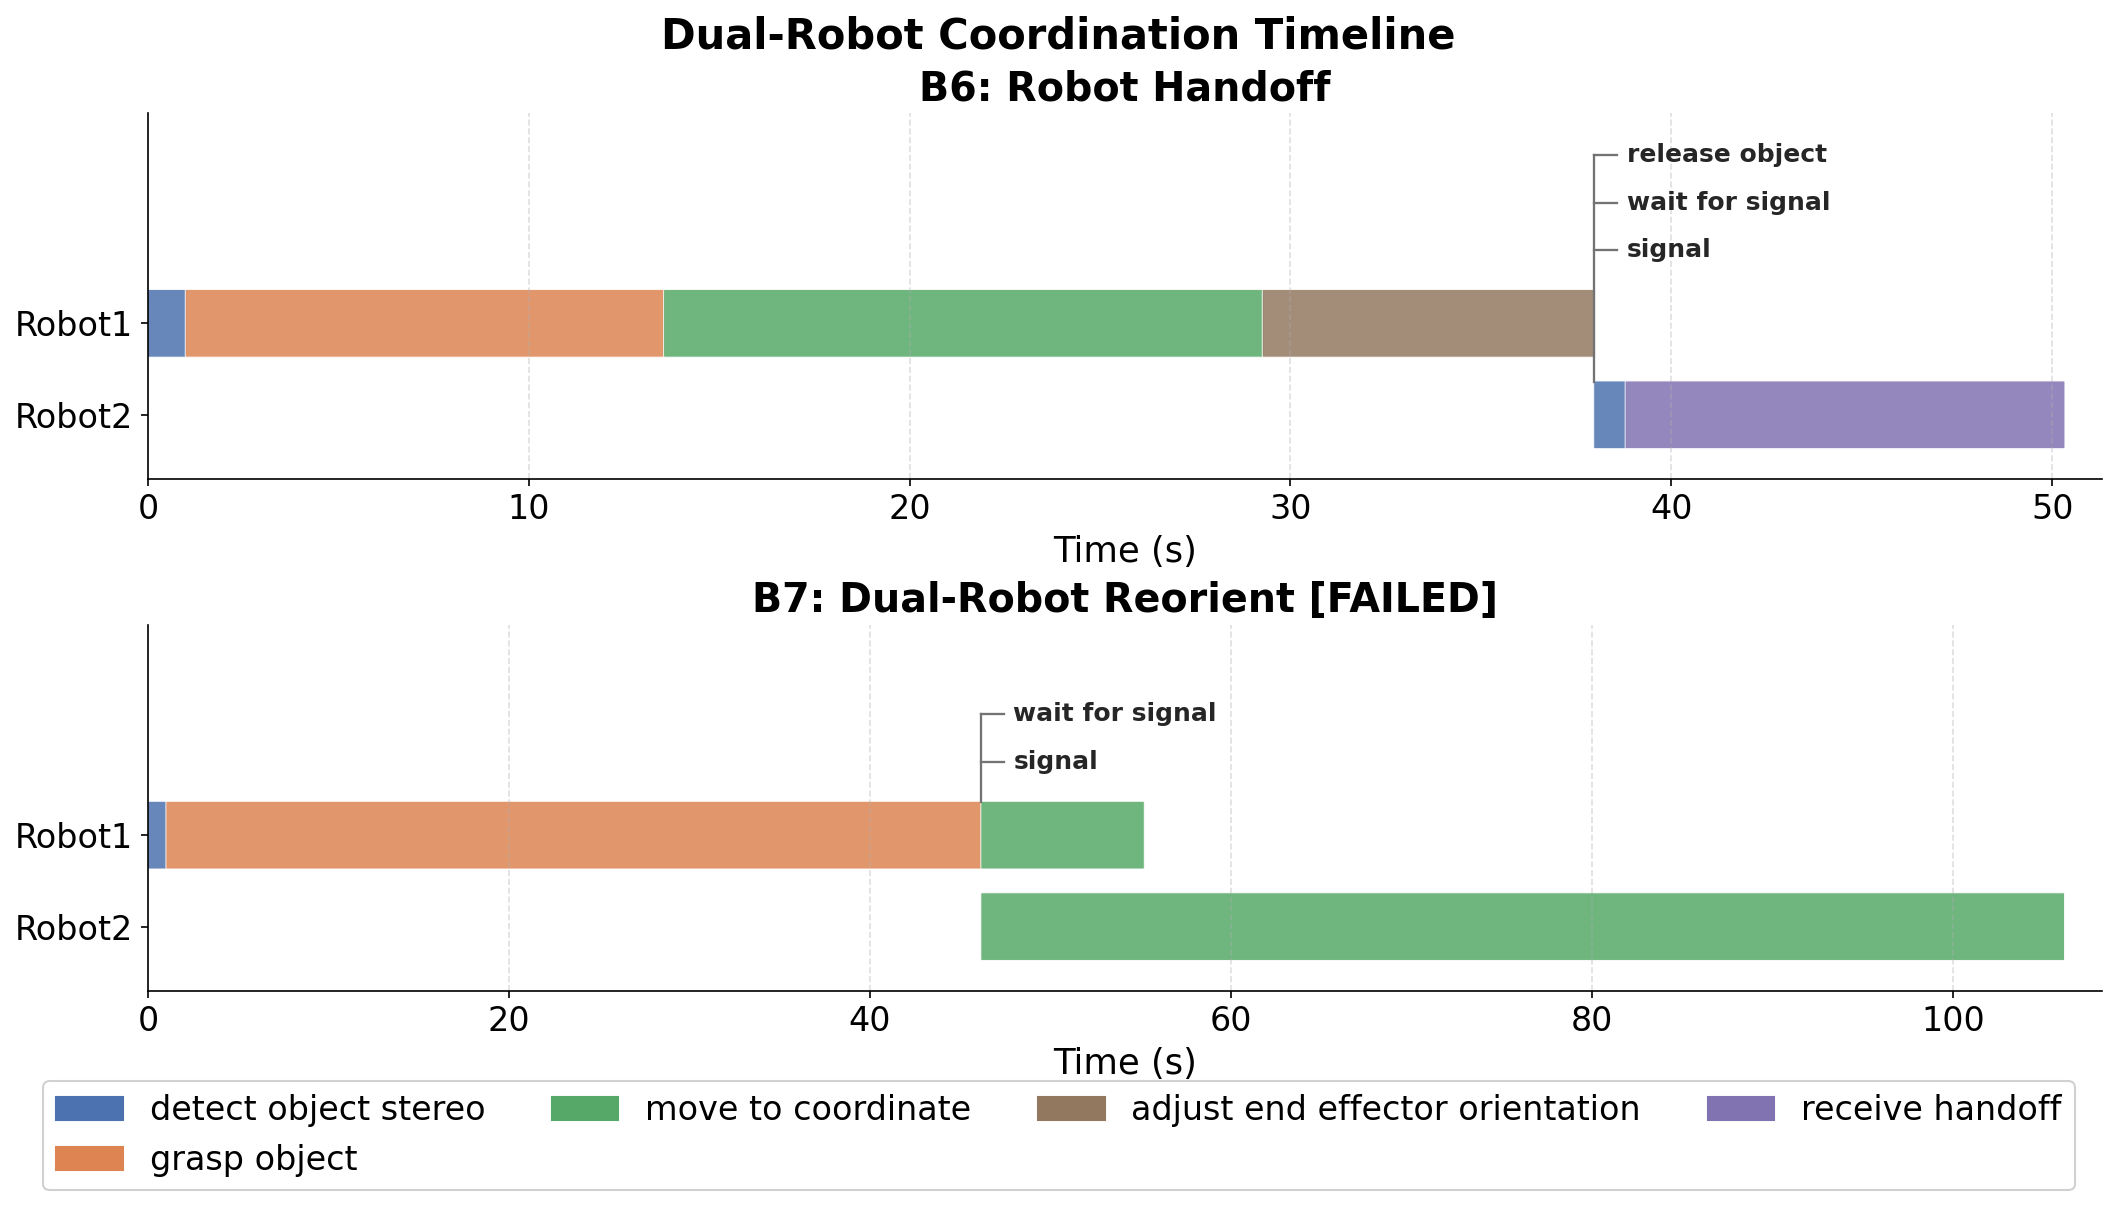
\includegraphics[width=1\linewidth]{images/07_coordination_timeline.png}
	\caption{Representative execution timelines for B6 and B7, both single \gls{magi} runs, not aggregates. The three instantaneous coordination operations (\texttt{signal}, \texttt{wait\_for\_signal}, and \texttt{release\_object}) carry no measurable duration, so they are indicated by labeled lines pointing to where each occurs on the relevant robot’s lane. In the successful handoff, Robot~2 starts its receive sequence only after Robot~1 has positioned and oriented the object. In the failed B7 run, the sequential plan leaves Robot~2 idle during Robot~1’s grasp; its subsequent \texttt{move\_to\_coordinate} is rejected by the workspace-separation check, with the two lift targets failing to meet the 0.2~m minimum.}
	\label{fig:coordination_timeline}
\end{figure}

\subsection{System Robustness}\label{sec:results-robustness}
Three benchmarks probe the system’s scaling properties. B8 tests whether the planner and execution stack remain reliable over a long heterogeneous chain spanning multiple robots and repeated cycles. B9 tests whether the parser correctly refuses physically impossible or semantically invalid instructions before any execution occurs. B10 tests whether the model planner recognizes task-level parallelism and reliably generates a concurrent execution plan; because the prompt supplies a general rule for co-grouping independent chains, B10 measures the dependable application of that rule. Together, they trace the limits of plan length, input robustness, and parallel scheduling.

\subsubsection{B8 — Heterogeneous Chain}
B8 is the most demanding benchmark in the suite; it structures each run as five cycles, each cycle containing four heterogeneous phases:

\begin{itemize}
	\item \textbf{Phase A}: \textit{Robot1: Grasp the blue cube and place it on field h, then return to start position}.
	\item \textbf{Phase B}: \textit{Robot2: Grasp the blue cube and place it on field b, then return to start position}.
	\item \textbf{Phase C}: \textit{Robot1: Grasp the blue cube and place it on field e, then return to start position}.
	\item \textbf{Phase D}: \textit{Robot1 and Robot2: Survey the scene. Robot1 should detect all visible fields. Robot2 should detect the yellow cube and report its current position}.
\end{itemize}

Each phase is issued as a separate natural-language prompt, yielding 20 sub-tasks and 85 operations per complete run. The system must plan, execute, and verify perception and manipulation for each prompt independently, without any cross-prompt memory.

The system completed all 20 sub-tasks across all five runs, with a per-step success rate of 1.000 and no hallucinated operations, retries, or reflection recoveries. All four phases achieved a success rate of 1.000 across every cycle of every run. Mean total duration was 26.7~min (\gls{sd} = 1.1~min). Under the benchmark’s own pass/fail criterion, the run is counted as successful only when each phase’s parsed operation chain matches the expected template exactly; by that rule, four of the five runs are recorded as successful, while the fifth is scored as unsuccessful solely because one phase’s plan deviated from that exact sequence. All 85 operations and all four phases still succeeded in that run. The backends separate sharply. \gls{magi} is the strongest, \gls{mini} and \gls{gema44} complete three of five each, and \gls{qwen38}, \gls{qwen330}, and \gls{gema42} fail every run either by truncating the per-phase plans or by accumulating chain-match deviations.

\begin{table}[t]
	\centering
	\begin{tabular}{lcc}
		\hline
		\textbf{Operation}                   & \textbf{Mean (ms)} & \textbf{\gls{sd} (ms)} \\
		\hline
		\texttt{detect\_object\_stereo}      & 855                & 65                     \\
		\texttt{grasp\_object}               & 31{,}530           & 10{,}718               \\
		\texttt{detect\_field}               & 743                & 32                     \\
		\texttt{place\_object}               & 61{,}245           & 14{,}339               \\
		\texttt{return\_to\_start\_position} & 9{,}811            & 1{,}200                \\
		\texttt{detect\_all\_fields}         & 925                & 34                     \\
		\hline
	\end{tabular}
	\caption{B8 per-operation mean latencies pooled across all five runs.}
	\label{tab:b8-latency}
\end{table}

The perception operations completed in under one second on average, with low variance (\gls{sd} $\le$ 65~ms), indicating that the deterministic stereo pipeline operates on stable scene configurations. The higher variance in \texttt{grasp\_object} and \texttt{place\_object}, as shown in Table~\ref{tab:b8-latency}, reflects the manipulation primitives’ sensitivity to where the cube and its target sit on each cycle. The grasp planner sees the blue cube at a different position each cycle, while \texttt{place\_object} descends to a different field target each time, so approach feasibility and descent distance vary accordingly.

\subsubsection{B9 — Impossible Task}
The task prompt is \textit{Robot3: Move the tree to the center}, and neither Robot~3 nor the tree object exists in the system. This benchmark tests whether the command parser correctly rejects physically impossible or semantically invalid instructions at parse time, instead of forwarding a plan that will fail at execution.

Only \gls{gema42} rejects the invalid prompt with any consistency (16 of 20 runs, a 0.80 rejection rate), and it does so by returning an empty parsed plan; its four acceptances emit a single command. \gls{qwen330}, which had refused all five of its original runs, rejects only 5 of 20 once resampled, emitting a full two- to three-operation plan for the impossible prompt in the other fifteen. The remaining models almost never reject: \gls{magi} and \gls{gema44} each refuse once in twenty, while \gls{mini} and \gls{qwen38} never refuse. Pooled across all six models, the parser rejects the invalid prompt in only 0.19 of runs. The harness runs B9 in parse-only mode, so no commands were dispatched and execution time was zero in every run.

Parse-level rejection is not a dependable guard for any model: even the best rejector refuses only four times in five. Rejection is also concentrated in the weakest planner. \gls{gema42} refuses most often precisely by failing to emit a plan at all, so its high score reflects capability-limited empty parses, not a deliberate, reasoning-based refusal; the stronger planners that can produce a plan almost always do, even for an unexecutable prompt. Checking against non-existent robots and non-graspable objects, therefore, cannot be delegated to the parser under any of these backends, and any safety guarantee against such inputs must be enforced by a downstream execution-layer guard or, better, a deterministic pre-parse validation step (Section~\ref{sec:parse-validation}) that is independent of model capability.

\subsubsection{B10 — Parallel Independent Tasks}
The task prompt is \textit{Robot~1: detect the blue cube, grasp it, and place it in field~A, and at the same time Robot~2: detect the green cube, grasp it, and place it in field~B}. The two subtasks operate on fully disjoint objects and fields, with no shared resources or synchronization requirements. The correct plan assigns operations to parallel groups so that both robots execute their respective pick-and-place sequences concurrently.

Reported for the default \gls{magi}, the system reached a task success rate of 1.000 across all five runs. All 40 operations executed successfully on the first attempt, with zero retries and zero hallucinated operations. Mean total duration was 61.7~s (\gls{sd} = 14.2~s), ranging from 44.2~s to 81.6~s. In every run, the model emitted a plan with a parallelism ratio of 0.75; six of the eight operations were assigned to three parallel groups. The two \texttt{detect\_object\_stereo} operations were scheduled sequentially, while the heavier manipulation operations were fully parallelized. Notably, the prompt’s independent-parallel exemplar co-groups the two detections; the model consistently serializes them instead, a benign deviation that still clears the $\geq 0.5$ criterion.

\begin{lstlisting}
detect_object_stereo (R1) -> detect_object_stereo (R2) -> [grasp_object  || grasp_object ] -> [detect_field  || detect_field ] -> [place_object  || place_object ]
\end{lstlisting}

\begin{table}[t]
	\centering
	\begin{tabular}{lcc}
		\hline
		\textbf{Operation}              & \textbf{Mean (ms)} & \textbf{\gls{sd} (ms)} \\
		\hline
		\texttt{detect\_object\_stereo} & 1{,}038            & 82                     \\
		\texttt{grasp\_object}          & 19{,}670           & 6{,}779                \\
		\texttt{detect\_field}          & 901                & 78                     \\
		\texttt{place\_object}          & 29{,}639           & 8{,}756                \\
		\hline
	\end{tabular}
	\caption{B10 per-operation mean latencies pooled across all five runs and both robots.}
	\label{tab:b10-latency}
\end{table}

The larger variance in \texttt{grasp\_object} and \texttt{place\_object} (Table~\ref{tab:b10-latency}) is consistent with pose-dependent approach selection. Robot~1 and Robot~2 operate on spatially separated objects throughout, so there is no contention between them. Prompted by the independent-parallel rule, the model recognized the two subtasks as independent and assigned the manipulation phases to matching parallel groups, so both robots execute concurrently. The outcome is model-dependent. \gls{mini}, \gls{qwen38}, and \gls{qwen330} likewise produced correct parallel plans at the same 0.75 ratio and reached a task success rate of 1.000, whereas both \gls{gema42} and \gls{gema44} failed B10, \gls{gema42} by planning sequentially and \gls{gema44} by intermittently emitting malformed duplicate-key plans.

\subsubsection{Summary}
B8, B9, and B10 mark out three independent robustness properties: the planner stays structurally reliable over long, heterogeneous chains (B8), parse-level rejection of invalid input is dependable for no backend (B9), and explicit task independence is correctly parallelized at a 0.75 ratio (B10). Their implications are taken up in Chapter~\ref{discussion}.

\subsection{Ablation Studies}
Benchmarks B11 through B16 isolate the contribution of individual architectural components by toggling a single feature flag while keeping all other conditions constant. Figure~\ref{fig:ablation_overview} previews each ablation’s main result; the subsections below give the full experimental design and analysis.

\begin{figure}
	\centering
	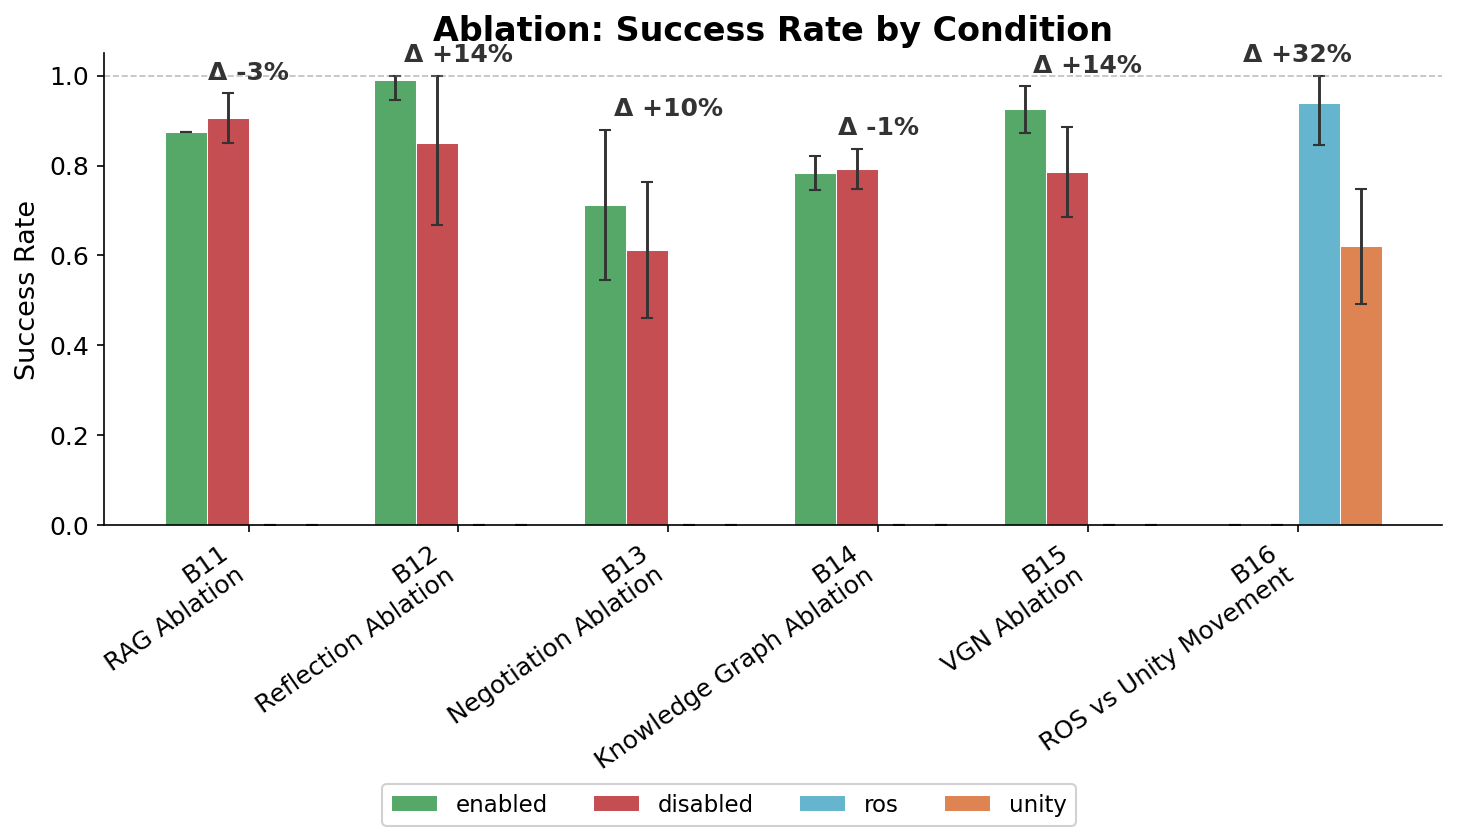
\includegraphics[width=1\linewidth]{images/08_ablation.png}
	\caption{B11–B16 ablation success rates for \textbf{\gls{magi} only} (per-model breakdown in Table~\ref{tab:combined_ablation_benchmark_runs}). Bars show per-task success by condition (enabled/disabled, or \gls{ros}/Unity for B16); twenty runs per condition for B11–B13 and B16 and five for B14–B15, error bars are the standard deviation across runs, and each $\Delta$ annotation is the enabled-minus-disabled gap. The B15 bars show the run-level success rate; scored on the stricter held-and-lifted grasp criterion used in the B15 analysis (Section~\ref{sec:results-vgn}), the enabled-minus-disabled gap widens to $+35$~pp (0.70 vs 0.35).}
	\label{fig:ablation_overview}
\end{figure}

\subsubsection{B11 — RAG Ablation}\label{sec:results-rag}
B11 isolates the contribution of \gls{rag} to operation selection precision. The \gls{rag} system improves the model prompt at parse time by retrieving the most semantically similar operation descriptions and workflow examples from the vector index. The ablation tests whether this retrieval step causally improves correct operation selection, or whether the model’s parametric knowledge alone is sufficient.

B11 consists of eight natural-language tasks (Table~\ref{tab:b11-tasks}), each deliberately ambiguous. Multiple operations from the registry could plausibly satisfy the description, but only one is correct given the system’s coordination semantics. We evaluated each task in two conditions, namely \gls{rag} enabled, where operation descriptions and usage examples are retrieved and prepended to the prompt, and \gls{rag} disabled, where the model receives the task prompt and the complete list of all registered operations with their parameter schemas and descriptions, but without retrieval ranking, relevant-subset narrowing, or workflow examples.

\begin{table}[t]
	\centering
	\resizebox{\textwidth}{!}{%
		\begin{tabular}{cp{9cm}l}
			\hline
			\textbf{\#} & \textbf{Task prompt}                                                                                 & \textbf{Ground truth}                       \\
			\hline
			1           & \textit{Request access to Robot2’s workspace region and wait until Robot2 has cleared it}            & \texttt{yield\_workspace}                   \\
			2           & \textit{The red cube is sitting on the table pick it up}                                             & \texttt{grasp\_object}                      \\
			3           & \textit{Put the block down exactly halfway between the blue block and the green block}               & \texttt{place\_between\_objects}            \\
			4           & \textit{Take the object that Robot1 is offering}                                                     & \texttt{receive\_handoff}                   \\
			5           & \textit{Before grasping, first check that you yourself aren’t already holding something}             & \texttt{check\_robot\_status}               \\
			6           & \textit{Map out every zone on the table before deciding where to place the object}                   & \texttt{detect\_all\_fields}                \\
			7           & \textit{Without moving from your current position, angle your gripper straight down over the object} & \texttt{adjust\_end\_effector\_orientation} \\
			8           & \textit{Do not move until you receive the go signal from Robot1}                                     & \texttt{wait\_for\_signal}                  \\
			\hline
		\end{tabular}
	}
	\caption{B11 task prompts and ground-truth operations. Each task is phrased with lexical overlap across several registered operations, so more than one could plausibly match, but only one is correct given the system’s operation semantics.}
	\label{tab:b11-tasks}
\end{table}

\begin{table}[t]
	\centering
	\begin{tabular}{llccc}
		\hline
		\textbf{Model}        & \textbf{RAG}                    & \textbf{Avg.\ correct / 8} &
		\textbf{Success rate} & \textbf{$\Delta$ vs.\ disabled}                                                   \\
		\hline
		\gls{magi}            & Enabled                         & 7.0                        & 0.875 & -          \\
		\gls{magi}            & Disabled                        & 7.3 $\pm$ 0.4              & 0.906 & $-3.1$~pp  \\
		\hline
		\gls{mini}            & Enabled                         & 5.7 $\pm$ 0.7              & 0.706 & -          \\
		\gls{mini}            & Disabled                        & 5.5 $\pm$ 0.6              & 0.681 & $+2.5$~pp  \\
		\hline
		\gls{qwen38}          & Enabled                         & 5.1 $\pm$ 0.7              & 0.631 & -          \\
		\gls{qwen38}          & Disabled                        & 6.0                        & 0.750 & $-11.9$~pp \\
		\hline
		\gls{qwen330}         & Enabled                         & 7.0                        & 0.875 & -          \\
		\gls{qwen330}         & Disabled                        & 7.0                        & 0.875 & $0$~pp     \\
		\hline
		\gls{gema42}          & Enabled                         & 1.0 $\pm$ 0.5              & 0.125 & -          \\
		\gls{gema42}          & Disabled                        & 2.8 $\pm$ 0.6              & 0.350 & $-22.5$~pp \\
		\hline
		\gls{gema44}          & Enabled                         & 6.2 $\pm$ 0.5              & 0.769 & -          \\
		\gls{gema44}          & Disabled                        & 6.8 $\pm$ 0.4              & 0.850 & $-8.1$~pp  \\
		\hline
	\end{tabular}
	\caption{B11 \gls{rag} ablation results across twenty repetitions per condition. $\pm$ denotes the \gls{sd} across the twenty repetitions; omitted where \gls{sd} = 0. $\Delta$ is the change in success rate when \gls{rag} is enabled relative to disabled; negative values indicate that retrieval degrades performance.}
	\label{tab:b11-results}
\end{table}

Retrieval does not improve operation selection for any model on this task set (Table~\ref{tab:b11-results}). At twenty repetitions per condition, no backend shows a clear gain. The two strongest models are effectively unaffected. \gls{qwen330} selects seven of eight in both conditions, and \gls{magi} shifts only $-3.1$~pp. For these, parametric knowledge appears to already cover the semantic distinctions the tasks probe, leaving little for retrieval to add. For the remaining three backends, retrieval is clearly net negative.

The negative cases do not follow either a clear scale or a clear family pattern. Within Qwen3, retrieval degrades the 8B model by $-11.9$~pp but leaves the 30B model unchanged, so the harm does not track parameter count. Both Gemma~4 models are also worse at retrieval; \gls{gema42} sits near the selection floor in both conditions ($-22.5$~pp), where the retrieved context appears to crowd out rather than sharpen the correct choice. Overall, retrieval helps no backend, is roughly neutral for three (\gls{mini}, \gls{magi}, \gls{qwen330}), and degrades three (\gls{qwen38}, \gls{gema42}, \gls{gema44}), pooling to $-7.2$~pp across all six models. Its parse-time contribution is therefore, on this task set, more often a cost than a benefit, which argues for enabling it per model.

\subsubsection{B12 — Reflection Ablation}\label{sec:results-reflection}
B12 evaluates the contribution of the reflection mechanism to task reliability. Reflection allows the system to detect a failed operation step, generate a corrective re-plan conditioned on the failure message, and re-attempt execution before reporting an overall failure. The ablation compares two conditions across 40 runs (20 per condition) on the same set of 5 tasks: with reflection enabled, where retry-and-replan is available after each failed step; and with reflection disabled, where a failed step propagates directly to a task failure. We deliberately constructed the five tasks to stress \gls{ik} reachability at workspace boundary coordinates, for example, $(-0.5, 0.08, 0.4)$ and $(0.5, 0.02, -0.4)$ and a low table-clearance height ($y = 0.02$~m), conditions under which initial \gls{ik} solutions are prone to failure. One task additionally involved an ambiguous natural-language reference, requiring a successful perception step before any motion could proceed.

\begin{table}[t]
	\centering
	\begin{tabular}{lcccl}
		\hline
		\textbf{Condition}  & \textbf{Task SR}      &
		\textbf{Op SR}      & \textbf{Duration (s)} & \textbf{Recoveries}              \\
		\hline
		Reflection enabled  & 99/100 (0.990)        & 0.996               & 202.1 & 20 \\
		Reflection disabled & 85/100 (0.850)        & 0.926               & 135.8 & 0  \\
		\hline
	\end{tabular}
	\caption{B12 reflection ablation results for \gls{magi} across twenty runs per condition. Per-operation success rate (Op SR) counts all individual operation attempts, including failed \texttt{move\_to\_coordinate} steps. Task SR counts completed tasks; a task counts as failed if any of its steps fail. Recoveries count step-level failures that the reflection mechanism retries successfully.}
	\label{tab:b12-results}
\end{table}

The reflection-enabled condition achieved a per-operation success rate of 0.996 (Table~\ref{tab:b12-results}) with 20 successful recoveries, while the disabled condition achieved 0.926 with 20 step failures, 13 in \texttt{move\_to\_coordinate} and 7 in \texttt{detect\_field}, spread across half its runs. At the task level, the disabled condition completed 85 of 100 tasks compared with 99 of 100 for the enabled condition, a 14-point gap that is larger than the 7-point per-operation gap because every unrecovered step marks its containing task as failed.

The disabled condition's failures concentrate in \texttt{move\_to\_coordinate}, dominated by boundary-coordinate moves that hit the sequence executor's 120-second per-step timeout; the robot's stale post-timeout position then resolves the following move to near-zero world coordinates and fails a spatial-feasibility check, so an affected run loses one or two movement steps. Reflection targets exactly this mode: it fired in 11 of the 20 enabled runs and recovered all but one of the failures, retrying the timed-out or infeasible step after re-parsing it with the failure message. The server logs confirm both the mechanism and its limit: most retries succeed, but a fraction of the spatial-feasibility rejections recur because the re-plan regenerates a similarly blocked coordinate. The single residual enabled-arm failure is one such case where both retries failed.

Recovery carries a clear and substantial latency cost. The nine enabled runs in which reflection never fired average 121~s, close to the disabled condition's failure-free runs (103~s), so the mechanism adds little when idle. But the eleven runs in which it fired average 268~s, roughly doubling the run time, because each recovery re-parses through the \gls{vlm} and re-executes the failed step on top of the 120-second timeout already spent, and a failed retry restacks that timeout. Reflection, therefore, buys the +14-point task-success gain at a recovery cost paid only on failure, but large when it occurs; this is examined further in Chapter~\ref{discussion}.

Across the wider model set, the effect stays non-negative for all but one backend, where it is within noise. Reflection lifts \gls{gema44} by 19~pp (0.78 to 0.97), \gls{magi} by 14~pp, \gls{gema42} by 10~pp, and \gls{mini} by 4~pp, while \gls{qwen330} is unchanged at 1.00 in both conditions and \gls{qwen38} dips a single point (0.99 vs 1.00), a one-run difference within run-to-run noise. \gls{qwen330} completes every task without a single retry, so the boundary-reach failure mode never arises; the models that improve are those whose disabled condition encounters that mode, and the benefit scales with how often it does (per-model runs in Table~\ref{tab:combined_ablation_benchmark_runs}).

\subsubsection{B13 — Negotiation Ablation}\label{sec:results-negotiation}
B13 evaluates the contribution of the \gls{vlm}-based negotiation mechanism to the reliability of dual-robot coordination. With negotiation enabled, the two robot agents execute a multi-round proposal-evaluation protocol before plan execution begins, jointly resolving role designation, sequential dependencies, and resource conflict. With negotiation disabled, a single model call must produce a complete dual-robot plan without inter-agent communication. The ablation uses four tasks we deliberately constructed to withhold per-robot role designations: retrieving the respective objects without explicit mapping, stacking one cube on another in unspecified order, a handoff task requiring negotiation between the initiator and receiver, and a two-stage sequential task with an implicit ordering constraint.

\begin{table}[t]
	\centering
	\begin{tabular}{lcccc}
		\hline
		\textbf{Condition}   & \textbf{Task SR}      &
		\textbf{Op SR}       & \textbf{Duration (s)} & \textbf{Ops executed (avg)}                \\
		\hline
		Negotiation enabled  & 57/80 (0.713)         & 0.855                       & 336.2 & 35.8 \\
		Negotiation disabled & 49/80 (0.613)         & 0.848                       & 298.9 & 29.9 \\
		\hline
	\end{tabular}
	\caption{B13 negotiation ablation results for \gls{magi} across twenty runs per condition (four tasks per run, 80 task instances each). Task SR counts completed tasks; the enabled condition completes 57 and the disabled 49, a $+10$~pp gap concentrated at the task level, as the per-operation rates are nearly equal (0.855 vs 0.848). Failed operations were predominantly \texttt{move\_to\_coordinate} (45 of the disabled failures, present in most runs) and \texttt{detect\_object\_stereo}, with \texttt{place\_object} and \texttt{release\_object} failing as downstream cascades.}
	\label{tab:b13-results}
\end{table}

Negotiation-enabled runs completed 57 of 80 tasks (Table~\ref{tab:b13-results}), compared with 49 of 80 for the disabled condition, a $+10$~pp task-level gap. These differences become clearer once the failure structure is examined. The gap does not appear at the per-operation level, where the two conditions are nearly tied (0.855 vs 0.848); it appears at the task level because failures in the disabled condition terminate task sequences early. Runs that abort stop short of their later, longer-running steps, which is why the disabled condition is also shorter on average (299~s vs 336~s) and executes fewer operations per run (29.9 vs 35.8): failed tasks cut off the more difficult later steps that are responsible for most failures, so the per-operation gap understates the reliability difference.

Without negotiation, the failures concentrate in \texttt{move\_to\_coordinate}, which accounts for 45 of the disabled failures and appears in most runs, with \texttt{detect\_object\_stereo}, \texttt{place\_object}, and \texttt{release\_object} failing alongside it, consistent with a single-model plan that sequences the two arms less reliably. Negotiation reduces but does not eliminate these failures, and it introduces its own: the coordination barriers it adds mean \texttt{signal} and \texttt{wait\_for\_signal} now fail in some enabled runs, and \texttt{place\_object} failures rise as more runs reach the later placement steps. Working back through the enabled runs in the server logs, we found why the net effect is nonetheless positive for this backend: negotiation is triggered in most of them, reaches consensus in roughly half, and on failure falls back to the single-shot command-parser path, so its downside is bounded while its successful rounds sequence the two arms enough to carry more tasks to completion.

The benefit is specific to \gls{magi} and does not generalize. Across twenty runs per condition, only \gls{magi} improves with negotiation ($+10$~pp, 0.713 vs 0.613). It is roughly neutral for three backends, \gls{gema44} ($+1$~pp), \gls{qwen330} ($-3$~pp), and \gls{mini} ($-4$~pp), and clearly negative for two, \gls{qwen38} ($-19$~pp) and \gls{gema42} ($-21$~pp). Pooled across all six models, it is a net cost ($-6$~pp). For the planners, the extra proposal-evaluation rounds do not resolve the role conflicts that defeat them, so the front-loaded cost buys little; negotiation pays off only when the single-shot plan is already close to correct (Table~\ref{tab:combined_ablation_benchmark_runs}). Tracing the same behavior across the other backends' logs confirmed this reading: wherever the logs capture the protocol, negotiation fires and reaches consensus at broadly similar rates (around 60 triggers per enabled condition), so the models it harms are not ones where negotiation mechanically fails but ones whose underlying plans it cannot rescue.

\subsubsection{B14 — Knowledge Graph Ablation}\label{sec:results-kg}
B14 evaluates the contribution of \gls{kg} spatial context enrichment to command-parsing quality. With the \gls{kg} enabled, each call to the model command parser is augmented with a context block derived from the \gls{kg}, with reachable objects and their distances, nearby robots, and candidate handoff paths, all computed from a synthetic spatial state populated via \texttt{populate\_synthetic\_kg}. With the \gls{kg} disabled, the parser receives only the raw natural-language task text and the standard operation schema. Each run exercises a single condition, selected via the \texttt{--no-kg} flag, against four tasks targeting spatial and handoff reasoning: nearest-object navigation, cube grasp-and-handoff, reachability-constrained lift, and inter-robot cube transfer. Both conditions are evaluated in dry-run mode; the parser produces an operation sequence, but no operations are dispatched to Unity.

\begin{table}[t]
	\centering
	\begin{tabular}{lccc}
		\hline
		\textbf{Condition}        & \textbf{Parse SR}   &
		\textbf{Bad ops}          & \textbf{Ops parsed}              \\
		\hline
		\gls{kg} context enabled  & 0.783               & 5.2 & 24.4 \\
		\gls{kg} context disabled & 0.792               & 4.4 & 21.8 \\
		\hline
	\end{tabular}
	\caption{B14 \gls{kg} ablation results. Parse SR is the mean fraction of parsed operations that are both a registered operation name and, for spatially-aware operations, reference a recognized object identifier or a variable substitution. Bad ops is the mean number of operations per run that fail either check.}
	\label{tab:b14-results}
\end{table}

B14 shows a small, consistent cost rather than a benefit (Table~\ref{tab:b14-results}). SR is 0.783 with the \gls{kg} enabled and 0.792 disabled, a 0.9 percentage-point gap that falls well inside the run-to-run spread of either condition at $n=5$. The bad-operation rate is marginally higher with \gls{kg} enabled (5.2 versus 4.4 per run), due to the same two failure modes in both conditions, with operation names absent from the registry and spatially-aware operations whose parameters reference neither a recognized object nor a variable. This residual rate is intrinsic to the parser/task combination, not to the spatial context. Across the six models, the effect is a small cost for five and marginally positive ($+1$~pp) for one, so no backend derives a clear parse-quality benefit from the context block (Table~\ref{tab:combined_ablation_benchmark_runs}).

\subsubsection{B15 — VGN Grasp Prediction Ablation}\label{sec:results-vgn}
B15 was designed to measure what the \gls{vgn} neural grasp-pose predictor adds to grasp reliability. \gls{vgn} replaces the geometric fallback planner with a learned model that scores candidate grasps using a volumetric occupancy representation derived from the stereo point cloud. In principle, it returns a full 6-DOF grasp pose, including the approach orientation, and not just a fixed top-down one. The ablation runs two conditions, \gls{vgn} enabled and \gls{vgn} disabled (the geometric top-down baseline), across the same four grasp-and-lift trials, five runs per condition. Each trial detects a cube, grasps it, lifts it toward $y = 0.2$~m, and re-detects; the four trials hit four different cubes at different positions and orientations, so the comparison spans a range of grasp geometries. A trial counts as a grasp success only when the object is actually held and lifted clear of the table (post-lift height above $0.1$~m), not just when the gripper-close command returns.

\begin{table}[t]
	\centering
	\begin{tabular}{lcccc}
		\hline
		\textbf{Condition} & \textbf{Grasp success} &
		\textbf{Op SR}     & \textbf{Duration (s)}  & \textbf{Avg.\ grasp (s)}                                   \\
		\hline
		\gls{vgn} enabled  & 14/20 (0.700)          & 0.925                    & 81.8 $\pm$ 8.1 & 13.9 $\pm$ 1.9 \\
		\gls{vgn} disabled & 7/20 (0.350)           & 0.790                    & 67.6 $\pm$ 4.9 & 11.8 $\pm$ 1.0 \\
		\hline
	\end{tabular}
	\caption{B15 \gls{vgn} ablation results for \gls{magi} (four grasp-and-lift trials per run). Grasp success counts the trials in which the object was held and lifted clear of the table; Op SR is the per-operation success rate. Duration values are per-run means $\pm$ \gls{sd}; Avg.\ grasp is the mean \texttt{grasp\_object} duration per run.}
	\label{tab:b15-results}
\end{table}

\gls{vgn} doubles grasp reliability. For \gls{magi}, the object is held and lifted in 14 of 20 trials with \gls{vgn} on, compared to 7 of 20 with the geometric baseline, yielding a $+35$~pp gap (Table~\ref{tab:b15-results}); per-operation success increases accordingly. Across all six models, the effect is model-independent: pooled over 30 runs and 120 grasp trials per condition, \gls{vgn} lifts the object in 90 of 120 trials versus 50 of 120 for the baseline ($+33$~pp), and every backend improves, consistent with the grasp-execution path (Table~\ref{tab:combined_ablation_benchmark_runs}).

The mechanism, on inspection, is not orientation, as both conditions command the same gripper orientation, a top-down pose whose yaw is aligned to the object’s long axis from the \texttt{WorldState} pose, applied identically whether \gls{vgn} is enabled or not. On the \gls{ros} path these runs take, \gls{vgn}'s own predicted orientation never reaches the executed grasp. Under this system’s sparse stereo \gls{tsdf}, \gls{vgn} predicts near-horizontal approach directions for tabletop cubes, which a vertical-component threshold screens out before planning (Section~\ref{sec:ros_moveit}), leaving the top-down heuristic in place. The difference between the two conditions lies in the grasp position. With \gls{vgn} enabled, the pipeline grasps at the detected object center; the geometric baseline grasps at its own computed contact point, which, on an angled cube, sits off-center. The centered grasp straddles the object and holds; the off-center one closes on a corner or an edge and lets the object slip. The Unity view is consistent with this. The enabled path contacts objects closer to their centers and holds visibly steadier. The enabled path is also somewhat slower, reflecting the added \gls{vgn} inference and candidate-validation overhead.

That the learned orientation is currently overridden does not make the \gls{vgn} path redundant; it is retained as deliberate sim-to-real infrastructure. The executed top-down orientation is a conservative placeholder standing in for \gls{vgn}'s predicted pose, kept in place for two reasons that are both properties of the simulated setup: the sparse, scale-biased \gls{tsdf} recovered from textureless simulated stereo (Section~\ref{sec:sim-to-real}) drives the network's predictions off-axis, and a top-down default keeps the reduced \gls{ik} solution space tractable for the planner while that input is degraded. A physical deployment changes the binding constraint. A dense, metrically accurate depth source behind the hardware adapter's existing depth hook would restore the reconstruction \gls{vgn} that was trained on, at which point its full 6-DOF pose could be planned and executed, and the placeholder override could be lifted. B15's $+33$~pp is thus what the path delivers through its positioning strategy alone, under degraded simulated depth and with the object position taken from the \texttt{WorldState} oracle rather than recovered from stereo; the benchmark isolates neither the learned 6-DOF pose nor stereo-derived position. Whether the network's learned orientation adds to that under real depth is a design hypothesis this simulation cannot test, but the pipeline is deliberately built to surface it once the perception supports it.

\subsubsection{B16 — ROS/MoveIt Integration Ablation}\label{sec:results-ros}
B16 evaluates the contribution of the \gls{ros}/MoveIt integration to task execution performance. With \gls{ros} movement enabled, \texttt{move\_to\_coordinate} and related motion operations are routed through MoveIt, which computes a collision-aware joint trajectory that Unity then executes. With \gls{ros} movement disabled, the same operations are dispatched directly to Unity via the TCP interface, where the built-in \gls{ik} solver and trajectory controller handle motion locally. The ablation uses the same five tasks as B1–B5.

\begin{table}[t]
	\centering
	\begin{tabular}{lcccc}
		\hline
		\textbf{Condition}    & \textbf{Task SR}        &
		\textbf{Duration (s)} & \textbf{Avg.\ move (s)} & \textbf{Avg.\ grasp (s)}              \\
		\hline
		\gls{ros} / MoveIt    & 0.940                   & 106.3                    & 4.8 & 16.5 \\
		Unity TCP             & 0.620                   & 48.0                     & 1.9 & 3.7  \\
		\hline
	\end{tabular}
	\caption{B16 \gls{ros}/MoveIt ablation results for \gls{magi} across twenty runs per condition. Task SR is the mean per-task success rate (\gls{ros}: fourteen runs at 1.000 and six at 0.800; Unity: five at 0.800, twelve at 0.600, three at 0.400). Unity \texttt{move\_to\_coordinate} completes in 0.8–3.0~s; the Unity grasp mean of 3.7~s is over the 24 grasps that completed and excludes the 31 \texttt{grasp\_object} timeouts (120~s step limit) that dominate the Unity failures. Duration values are per-run means.}
	\label{tab:b16-results}
\end{table}

Mean task success is 0.940 for \gls{ros} (fourteen runs at 1.000 and six at 0.800, $n = 20$) against 0.620 for Unity (three runs at 0.400, twelve at 0.600, five at 0.800), a $+32$~pp gap (Table~\ref{tab:b16-results}). The two conditions fail in different ways. All six \gls{ros} failures are \texttt{detect\_object\_stereo} misses of the blue cube, and detection misses are comparable across conditions (six under \gls{ros}, seven under Unity), so perception does not separate the two paths. What separates them is manipulation execution: the Unity condition incurs 38 failed task instances against 6, and 31 of the 38 are \texttt{grasp\_object} timeouts due to the 120~s step limit, with the remaining 7 being detection misses. These grasp timeouts never occur under \gls{ros}: across all 45 \gls{ros} runs in the six-model sweep, not a single \texttt{grasp\_object} or \texttt{place\_object} timeout is recorded, whereas manipulation-execution timeouts appear under Unity for five of the six backends (40 grasp-or-place timeouts across the 45 Unity runs), confirming the effect is a property of the routing path. The mechanism is in the direct-path \gls{vgn} routing (\texttt{operations/grasp/\_vgn.py}): unlike the \gls{ros} path, the Unity path forwards raw 6-DOF candidate orientations to Unity without the top-down candidate selection and \texttt{WorldState} position/orientation override that the \gls{ros} path applies, so the gripper approaches the cube from the side and the local grasp controller fails to converge before the step times out.

Per-operation timings are only loosely comparable because both conditions execute physics in Unity (MoveIt is plan-only), but differ in trajectory shape and completion semantics. The \gls{ros} path follows a full collision-aware joint-space plan and blocks until Unity reports trajectory completion (move 2.7–12.5~s), whereas the direct path executes a Cartesian point-to-point move and returns once the controller signals that the target has been reached (0.8–3.0~s). MoveIt as the default is justified both by its collision-aware \gls{ompl} planning, which can find collision-free trajectories that point-to-point \gls{ik} cannot represent, and by the measured grasp-execution reliability gap above.

\subsubsection{Cross-Ablation Synthesis}\label{sec:results-ablation-synthesis}
The six ablations act on three different outcome axes, so their effects compare only within an axis, not across axes: task-level success (reflection, negotiation, \gls{ros}/MoveIt routing), grasp reliability (\gls{vgn}), and parse quality (\gls{rag}, \gls{kg}). Ranked within each, \gls{ros}/MoveIt routing is the largest task-success effect (B16, $+32$~pp), ahead of reflection (B12, $+14$~pp) and negotiation (B13, $+10$~pp); \gls{vgn} is the largest grasp effect (B15, $+33$~pp pooled); and on parse quality both \gls{rag} and the \gls{kg} are net costs. The six-model sweep separates the general effects from the conditional ones: the \gls{ros} routing gap and \gls{vgn}'s grasp gain hold across all six backends, whereas reflection helps four of six and negotiation only \gls{magi} (net $-6$~pp pooled), so the task-success gains are backend-conditional while the execution-path effects are not.

Each positive component targets a specific failure class: reflection retries, transient \texttt{move\_to\_coordinate} timeouts, and spatial-feasibility rejections. Negotiation resolves conflicting role allocations at a cost small relative to the physical execution time it protects. The two parse-quality components pay off on neither: \gls{rag} is a net cost whose size is model-dependent, and the \gls{kg} imposes a small but consistent one as the model over-anchors on the spatial context and emits out-of-schema operation calls, a prompt-integration failure whose redesign Chapter~\ref{discussion} takes up.

\subsection{Autonomous Task Generation and Safety}\label{sec:results-autort}

The benchmarks above exercise the execution path; B17 tests AutoRT’s own stages instead, the task generator and the two-layer Robot Constitution (Section~\ref{sec:autort}), driven directly and fully offline (Section~\ref{sec:benchmark-impl}). Like B11 and B14, it dispatches nothing to Unity, but it is even more self-contained, bypassing the command parser entirely. We ran it five times per model across all six backends, reporting \gls{magi} as the headline (per-model runs in Appendix~\ref{appendix:benchmark_runs}).

B17 measures two properties. The first is the safety gate. We feed a hand-labeled task set to the Robot Constitution. Each set pairs clearly safe and clearly unsafe tasks with boundary cases. We then score the accept/reject verdicts against the labels (Table~\ref{tab:b17-results}). Every run returned the same confusion matrix: 11 true rejects, 2 false rejects, 6 true accepts, and 0 false accepts across 19 tasks. This yields an accuracy of 0.895. The error profile is conservative by construction. The false-accept rate was 0.000, so the gate did not admit an unsafe task, even at the limit boundary. The false-reject rate was 0.250, reflecting safe but aggressively phrased in-limit tasks that the gate over-rejected. Splitting the verdicts by layer, the kinematic code check was exact, and the semantic \gls{vlm} layer caught every unsafe case routed to it but over-rejected two safe, aggressively phrased tasks. That over-rejection is the gate’s only miscalibration, and it stems from the semantic layer’s handling of borderline-safe phrasing, not from the kinematic guarantees. The gate’s conservatism is shared but not identical across models. The four stronger backends (\gls{magi}, \gls{mini}, \gls{qwen38}, \gls{qwen330}) reproduce \gls{magi}'s exact 0.895 accuracy and 0.000 false-accept rate, while both Gemma~4 models over-reject more aggressively (accuracy 0.789, false-reject rate 0.500). Critically, the false-accept rate is 0.000 across all six models, so the model choice trades only against over-rejecting safe tasks, never against safety.

The second property is generation quality: how reliably AutoRT’s generator produces a valid task. The generator fills a fixed set of parallel slots per scene, each an independent generation attempt; the benchmark widens the live loop’s default of two slots per scene (Section~\ref{sec:autort-impl}) to 24, giving 48 per run across the two evaluation scenes. Its \texttt{generate\_tasks} entry point deduplicates results by task identifier, but the model assigns every slot the same identifier, so deduplication collapses all valid candidates into a single candidate and makes the naive \textit{yield} metric badly understate the true output. We therefore measure at the slot level, before deduplication, using two rates, namely slot success, the fraction of slots that eventually yield a valid task within the retry budget, and first-attempt validity, the fraction that are valid on the first attempt. For \gls{magi}, slot success was 0.992 (per-run 0.979–1.000) and first-attempt validity 0.804 (0.688–0.875). Four in five drafts are valid immediately, and because retries clear almost all of the rest, slot success ultimately reaches roughly 0.99. First-draft rejections come mostly from reachability and field-rule violations, with occasional malformed parameters. The diversity metrics confirm that the collapse is a measurement artifact and not a generation failure. The generated operation chains are structurally varied (op-chain diversity 0.29–0.58) while task-identifier diversity is near zero. Across models, first-attempt validity ranges from 0.329 (\gls{gema42}) to 1.000 (\gls{qwen38}), and slot success stays high (0.971–1.000) for every backend except \gls{gema42} (0.838), so \gls{magi}'s 0.804 sits toward the lower end (per-model runs in Appendix~\ref{appendix:benchmark_runs}).

\begin{table}[t]
	\centering
	\begin{tabular}{lc}
		\hline
		\textbf{Metric}                        & \textbf{Value}      \\
		\hline
		Safety-gate accuracy                   & 0.895 (17/19)       \\
		False-accept rate                      & 0.000               \\
		False-reject rate                      & 0.250               \\
		Semantic-layer recall (unsafe caught)  & 1.000 (4/4)         \\
		Kinematic-layer recall (unsafe caught) & 1.000 (7/7)         \\
		Generation slot success                & 0.992 (0.979–1.000) \\
		First-attempt validity                 & 0.804 (0.688–0.875) \\
		\hline
	\end{tabular}
	\caption{B17 AutoRT results (\gls{magi}, $n=5$). Safety-gate figures are identical across all five runs (semantic layer at temperature~0); generation figures are means with per-run ranges over 48 slots per run.}
	\label{tab:b17-results}
\end{table}


%%%%%%%%%%%%%%%%%%%%%%%%%%%%%%%%%%%%%%%%%%%%%%%%%%%%%%%%%%%%%%%%%%%%%%%%%%%%%%%%
%%  DISCUSSION AND LIMITATIONS
%%%%%%%%%%%%%%%%%%%%%%%%%%%%%%%%%%%%%%%%%%%%%%%%%%%%%%%%%%%%%%%%%%%%%%%%%%%%%%%%
\chapter{Discussion and Limitations}\label{discussion}
The benchmark results show that the framework reliably translates natural-language instructions into coordinated actions. At the same time, the runs expose recurring failure modes and several open design questions. Together, these restrictions define the system’s usefulness today and set the agenda for the rest of this chapter.

% ------------------------------------------------------------------------------
\section{Perception and Depth Sensing}\label{sec:perception-depth}
The tuned \gls{sgbm} pipeline localizes objects under 1~m to within 5–10\% depth error, and this per-object depth estimate is robust. Taking object depth as the median disparity over the textured detection region averages out the zero-mean matching noise. That robustness does not carry over to the dense, per-pixel depth that \gls{vgn} requires. \gls{vgn}'s volumetric occupancy grid is built by back-projecting the full disparity map, and on the textureless surfaces that dominate the scene, per-pixel stereo matching fails systematically. Because that error is a systematic scale bias, median aggregation, which rescues object localization, cannot correct it. The result is sparse, discontinuous \gls{tsdf} volumes that mislead the grasp-quality network into predicting off-axis candidates or suppressing valid poses.

The heuristic geometric planner, therefore, acts as a conditional fallback, not the intended primary grasp source. It fires precisely when \gls{vgn} cannot return a usable pose, which is the common case here but reflects the degraded stereo input. The fallback itself is robust: it needs no dense 3D reconstruction, avoids the scale bias entirely, scores candidates on direction, contact geometry, and \gls{ik} quality, and always issues and closes a grasp.

Even so, the \gls{vgn} path is not abandoned. In simulation, it does not bypass the stereo sensor: its occupancy grid is built from the same \gls{sgbm} point cloud used for real images, and to work around the scale bias, the object position is taken from the simulator’s \texttt{WorldState} oracle rather than recovered from that cloud. A dedicated depth sensor behind the adapter’s existing \texttt{get\_depth\_frame} hook would supply that localization at the source and let an actual \gls{vgn} pose contribution be recovered, a deployment prerequisite we return to in the next chapter.

% ------------------------------------------------------------------------------
\section{Large Language Model Latency as a Control Bottleneck}
As Section~\ref{sec:communication} notes, end-to-end command latency breaks into three components, and \gls{vlm} parsing dominates. It is also the least predictable component: a short, unambiguous prompt parses in under 10~s, while a multi-robot task requiring complex coordination consumes the full thinking budget and approaches the 90-second request timeout.

This latency profile has two practical consequences. First, it precludes reactive control. The system cannot re-plan faster than the model generates tokens. A robot moving at 0.5~m/s travels 10~m during a median-length parse, so any obstacle or object displacement that occurs while the planner thinks is invisible to it. Replanning is therefore viable between motions, never during one. Second, planning cost and execution cost are decoupled. The negotiation protocol front-loads a single analysis–proposal–evaluation round of model calls per task, while leaving the per-operation execution rate unchanged. The longer wall-clock totals for the negotiation-enabled runs, therefore, reflect more completed work rather than slower planning and should not be read as a planning-speed effect.

% ------------------------------------------------------------------------------
\section{Inverse Kinematics Convergence at Workspace Boundaries}
The damped least-squares \gls{ik} solver converges reliably within the core of each robot’s reachable workspace but degrades near the boundary, where the Jacobian becomes ill-conditioned at near-singular configurations. The damping factor $\lambda = 0.2$ suppresses the most severe inversions, yet it cannot eliminate convergence failures for targets that fall exactly at the reachable radius or demand approach trajectories through kinematic singularities. Boundary targets thus remain intrinsically fragile even when the solver is tuned conservatively.

This degradation is an analytical property of the direct-\gls{ik} path, not something the benchmarks isolate, since the ablations toggle reflection and \gls{ros} movement, not the \gls{ik} solver alone. The B12 reflection ablation shows that transient motion failures at boundary coordinates occur and usually recover on a retry; because those moves were planned through \gls{ros}/MoveIt, they reflect transient planning and execution failures, not steady-state direct-\gls{ik} convergence. The practically important point is the non-determinism. Identical task sequences succeed in some runs and fail in others, an intermittent \textit{sometimes fails} error class that restricting command coordinates alone cannot guard against.

As B16 establishes, the advantage of \gls{ros}/MoveIt here is both capability and reliability. Its full-joint-space \gls{ompl} planning finds collision-free trajectories that direct \gls{ik} cannot, and its grasp routing avoids the direct path's side-approach failures (Section~\ref{sec:results-ros}). Extending this collision-aware planning from point-to-point motion to the full grasp pipeline is thus the clearest path to improving task robustness, since it directly reduces workspace-boundary and approach failures.

% ------------------------------------------------------------------------------
\section{Bimanual Manipulation and Synchronized Grasping}\label{sec:bimanual}
B7’s failure is easy to misdiagnose, so it is worth stating what the task asks for: a sequential two-arm grasp, each \texttt{grasp\_object} bracketed by a \texttt{signal}/\texttt{wait\_for\_signal} barrier, followed by a simultaneous lift to $y=0.15$~m. The two failure modes documented in Section~\ref{sec:results-dual}, the mis-realized barrier and the lift rejection, are therefore not missing operations. What the lift phase reveals is a lack of partner-aware target selection: each robot independently determines its end-effector target, so two valid lift poses can still collide, and the violations cluster tightly around 0.10–0.11~m.

A deeper, simulation-level constraint prevents genuine concurrent dual-grasping of a single object, regardless of target selection. The reparenting is itself a workaround. Friction-only grasping in Unity’s physics engine proved unreliable, with objects slipping or jittering out of the gripper, so on grasp \texttt{GripperController} rigidly attaches the object to the gripper transform via \texttt{SetParent} instead of relying on contact friction. A Unity~\cite{unity} \texttt{Transform} admits exactly one parent, however, so one object cannot attach to two grippers at once. The handoff path works only because it serializes. Before the second gripper attaches, it forces the first to release. This is also a reliability hazard: the receiver only re-parents once its attachment check succeeds (gripper within about 10~cm of the object), so if the source releases while the object is outside that window, it reverts to a friction-only hold and can fall onto the table. A true co-grasp would therefore require replacing the single-parent attachment model itself as a second blocker, independent of the missing partner-aware target selection.

Because these blockers are independent of the planner, B7 is partially unwinnable regardless of the plan’s quality. The run data still separates two outcomes worth keeping distinct. The planner reproduced the expected chain only approximately. Plan length varied from 7 to 10 operations, and 3 of the 5 \gls{magi} runs dropped the second synchronization barrier. The coordination safety layer, by contrast, worked as intended. Notably, the \texttt{SetParent} ceiling is never actually reached. Execution halts earlier at the handshake or the proximity check, so the attachment limit stays theoretical here. A benchmark that genuinely tests co-grasping would need either a dual-attachment representation or a configurable physics joint in place of the single reparenting transform, or it would score the lift based solely on target selection.

% ------------------------------------------------------------------------------
\section{Parse-Level Input Validation}\label{sec:parse-validation}
B9 shows that parser-level rejection of impossible instructions is unreliable for every model, as no backend rejects with any consistency except the weakest planner (\gls{gema42}), and it does so only by failing to emit a plan at all (Section~\ref{sec:results-robustness}).

This is not inherently unsafe. Because B9 stops at parse time (Section~\ref{sec:results-robustness}), no motion is dispatched, and at execution, the precondition and coordination guards would reject commands referencing an unknown robot or a missing object. But for models that do not reject at parse time, the safety guarantee against invalid inputs rests entirely on those downstream guards. A prompt that names a valid robot and object but combines them in an impossible way would likewise reach the execution layer and fail only at the grasp step, after wasting time on detection, motion, and contact verification.

A dedicated pre-parse validation step that checks robot identifiers against the registered robot set and object IDs against the live world state would catch the B9 class of errors deterministically before any model call and independently of model capability. The Robot Constitution already establishes the pattern of code-level pre-execution checks on AutoRT-generated tasks, but it validates kinematic constraints rather than identifier or object existence; extending it with those membership checks, applied to externally submitted commands, is the missing piece to close this benchmark limit.

% ------------------------------------------------------------------------------
\section{Knowledge Graph Context Injection}
B14 found that \gls{kg} context injection carries a small, consistent cost. It lowers parse-level success by about 1~pp and adds close to one flagged operation per run, on top of a disabled baseline that already carries 4–5 flagged operations per run. The graph, therefore, does not create hallucination where none existed; it slightly aggravates a residual floor that is already present and intrinsic to the parser/task combination.

The benchmark cannot localize this cost further, because it records a single combined count that sums two distinct checks, namely operations absent from the registry entirely, and \gls{kg}-aware operations whose parameters reference neither a \gls{kg} object id nor a \texttt{\$variable}. No intermediate condition separates the effect of the added prompt structure from that of the spatial facts’ semantic content, so the two cannot be told apart from this result alone.

Because that floor is independent of the graph, the targeted-injection redesign proposed in future work should be motivated by reduced prompt load rather than by the prospect of eliminating it.

% ------------------------------------------------------------------------------
\section{Simulation-to-Real Gap}\label{sec:sim-to-real}
The system is developed and validated entirely within Unity’s \texttt{ArticulationBody} simulation. Several properties of this environment do not transfer directly to a physical AR4 installation, as physical robot joints exhibit compliance, backlash, and friction that the \texttt{ArticulationBody} model does not reproduce, so the simulation-tuned \gls{pd} gains will need to be retuned against the real AR4’s inertia and damping for deployment.

Grasp verification compounds this deployment gap. In simulation, grasp force is read from the finger \texttt{ArticulationBody} joint forces and smoothed with a 5-frame moving average; the 5~N minimum-force threshold and 50~ms contact-duration requirement were tuned to reject simulation physics noise, not real fingertip normal forces, which depend on surface material, object deformability, and approach speed. Both must be revalidated against the real robot’s force response.

Object state is the larger substitution. Because the synthetic stereo overestimates depth by roughly 1.8$\times$ on Unity’s textureless surfaces, the grasp path reads object position, dimensions, and orientation from the simulator’s \texttt{WorldState} oracle instead of the point cloud (Section~\ref{sec:perception-depth}). \texttt{WorldState} is the interface a real perception stack would populate in its place. Detection already writes stereo-derived position back to it, so position closes with the depth-sensing upgrade; dimensions and orientation have no perception producer today and would need a segmentation-and-pose capability that the system does not yet build, not merely a better sensor.

The hardware adapter layer makes this deployment a configuration change. The adapters expose the same abstract interface as their Unity equivalents, so no operation code changes when switching modes. Motion is routed through the \gls{ros}/MoveIt backend, so trajectory execution on the physical AR4 depends on its \gls{ros} driver alone. Perception is already wired end-to-end. A capture bridge forwards the local camera adapter’s frames into the same image store that the pipeline reads in simulation. What remains is integration and validation on real hardware, namely depth sensing, force-torque feedback (currently used as a contact-duration heuristic), camera calibration, and validation on the real arms.

% ------------------------------------------------------------------------------
\section{Evaluation Scope and Coverage}
The B12 reflection benefit is real, and at twenty runs per condition, its latency cost is measurable. That cost falls entirely on the runs that fail: a disabled run that aborts at the 120-second per-step timeout averages 168~s, and enabling reflection roughly doubles a firing run's duration on top of that (Section~\ref{sec:results-reflection} breaks down the fired-versus-idle timings). This sharpens the trade-off: reflection reliably converts intermittent boundary-reach failures into successes ($+14$~pp task success) but is expensive precisely on the runs that need it most, where recovery latency is bounded.

Two coverage gaps remain. First, the evaluation cannot assess reflection over longer deployment windows or densely coupled task sequences. The five stress tasks were mutually independent, so an unrecovered failure cost only its own task, whereas in a tightly coupled sequence, a single failure would cascade downstream, and the mechanism’s value would be correspondingly larger. Second, B17 exercises only AutoRT’s own stages, the task generator, and the two-layer Robot Constitution, offline and in isolation. The full generate–filter–select loop, running end-to-end against a live, changing scene, remains unevaluated, and with it, selection-strategy behavior over long horizons, proposal diversity under repeated execution, and the constitution’s rejection profile as the scene evolves. Both regimes would first require defining success criteria for open-ended task generation, an open research question in itself.

Underlying all of these is the run budget. Most conditions were evaluated five times in a single simulated environment, with the B9, B11–B13, and \gls{magi} B16 sweeps extended to twenty; five runs is enough to expose deterministic failure modes but not to resolve small effects that lie within one \gls{sd}. A fuller evaluation would need more runs, harder tasks, hardware-in-the-loop testing, and injected faults to sharpen the latency takeaway.


%%%%%%%%%%%%%%%%%%%%%%%%%%%%%%%%%%%%%%%%%%%%%%%%%%%%%%%%%%%%%%%%%%%%%%%%%%%%%%%%
%%  CONCLUSION
%%%%%%%%%%%%%%%%%%%%%%%%%%%%%%%%%%%%%%%%%%%%%%%%%%%%%%%%%%%%%%%%%%%%%%%%%%%%%%%%
\chapter{Conclusion}\label{conclusion}
We set out to show that a locally hosted model, grounded in a structured set of basic operations, can translate natural-language instructions into reliable, coordinated behavior across two robot arms without specialized training or hard-coded sequencing. The main takeaway is that our results support that claim across a broad range of tasks, while also marking the limits of the current implementation.

% ------------------------------------------------------------------------------
\section{What the System Accomplishes}
The system’s central pipeline works end-to-end. A single instruction flows through \gls{rag}-augmented retrieval, \gls{vlm} plan generation with chain-of-thought grounding, sequence-executor dispatch with variable-passing resolution, and physical execution in Unity. With the \gls{magi} backend, single-robot tasks achieved a 1.000 success rate across all 25 runs, and the B6 handoff across all 5 runs, with zero hallucinated operations and zero retries. These results show that the system can reliably turn language into coordinated action, and the dominant cost is contact-rich physical manipulation.

The pipeline composes its coordination at the planning layer rather than in the executor. Signal/wait synchronization points, parallel-group assignments for independent sub-tasks, and re-detection before each manipulation step are all generated by the \gls{vlm}; none is scripted into the executor, though the default prompt supplies rules that guide them. B10 illustrates this clearly, as the \gls{vlm} identified task-level independence between two disjoint pick-and-place subtasks and scheduled the grasp, field-detection, and placement phases into three concurrent groups while serializing the initial detections.

B8 stress-tests durability over a sustained multi-cycle sequence, and execution was flawless across all five runs with no cascading errors. The one run that scored as a failure missed only the benchmark’s exact chain-match check, despite identical execution. The main takeaway is sustained execution reliability, while op-level correctness and exact-sequence fidelity are scored separately.

Concurrent physical coupling marks the current capability boundary. Every model fails the simultaneous lift. The exposed failures are mis-realized cross-robot synchronization barriers and partner-aware target selection at the lift. The co-grasp itself is additionally blocked by the simulator’s single-parent attachment model (Sections~\ref{sec:results-dual} and~\ref{sec:bimanual}). This is the clearest remaining limitation.

Among the ablations, \gls{ros}/MoveIt routing showed the largest task-success gap, followed by reflection and negotiation. Reflection generalizes, helping or leaving the backend neutral, while negotiation helps only the default one; B16's gap, by contrast, is model-independent, tracing to \texttt{grasp\_object} timeouts that occur only under direct Unity routing, never under \gls{ros} for any model. On the grasp axis, the \gls{vgn} grasp path shows the largest and most general reliability effect, holding across all backends; an execution-path audit attributes it to grasp positioning and not \gls{vgn}'s predicted orientation (Section~\ref{sec:results-vgn}), whose own contribution awaits the depth-sensing upgrade below. \gls{rag} is model-dependent and, on the current task set, nets negative more often than it helps, and the \gls{kg} carries a small, consistent cost.

% ------------------------------------------------------------------------------
\section{Key Contributions}
The five contributions previewed in Section~\ref{sec:novelty} are realized and substantiated by the evaluation. The retrieval-grounded operation pipeline, a locally hosted reasoning model over a hierarchical 20-operation registry with \gls{rag} retrieval, an RT-H-style~\cite{belkhale2024rthactionhierarchiesusing} two-phase decomposition, and runtime variable-passing, decouples planning from execution without fine-tuning and underpins every benchmark in the suite. On top of that, the model coordinates the dual arms at the planning layer. The three optional layers each contribute a measurable, separately evaluated effect: consensus-gated negotiation, operation-gated reflection, and the AutoRT~\cite{ahn2024autortembodiedfoundationmodels} adaptation that pairs a structured object manifest with a hard kinematic safety layer the semantic filter cannot override. Together, the benchmarks confirm the central claim. Coordinated dual-arm behavior can be composed at runtime using a shared vocabulary of operations.

% ------------------------------------------------------------------------------
\section{Path to Deployment and Future Work}
The hardware adapter boundary analyzed in Section~\ref{sec:sim-to-real} enables the switch to hardware. The \texttt{--env real} flag selects the real-robot adapters, and the \gls{ros}/MoveIt path, \gls{ros}-TCP bridge, topic namespaces, and camera capture are already configured for dual-robot operation. What remains is the integration and validation: executing the planned trajectories on the physical AR4 \gls{ros} driver, calibrating the real cameras, and closing two sensing gaps, namely depth sensing, on which \gls{vgn}-quality grasp prediction depends via the existing \texttt{get\_depth\_frame} hook, and force-torque feedback, which would replace the contact-duration heuristic with ground-truth contact measurement.

Beyond those two hardware gaps, several further directions remain, following from the benchmark findings and the limitations identified in the last chapter.

\paragraph{Depth sensing upgrade.} Replacing the stereo pair with an active-stereo or time-of-flight depth sensor would make \gls{vgn}-based grasp planning reliable by supplying the dense, millimeter-level per-pixel depth that the current stereo reconstruction degrades on. It would also remove the current reliance on the simulator's \texttt{WorldState} oracle for object position, dimensions, and orientation (Section~\ref{sec:sim-to-real}), which a physical installation cannot provide, making this the gating prerequisite for real-world grasp localization.

\paragraph{Persistent spatial mapping.} Perception is currently memoryless. Every detection rebuilds the scene from a single stereo pair, with no spatial model carried across viewpoints or over time. Fusing the depth source above into a persistent volumetric map using Simultaneous Localization and Mapping (SLAM) or \gls{tsdf} fusion would give the planner object permanence under occlusion, multi-view grasp reconstruction, and a consistent workspace frame shared by both arms. It is also a prerequisite for moving beyond a fixed base.

\paragraph{Partner-aware target selection.} When B7’s execution reaches the concurrent lift, it fails because each arm resolves its own end-effector target in isolation, so two individually valid targets can land inside the 0.2~m separation check. The direct fix is a compatibility check at the lift. Before either \texttt{move\_to\_coordinate} commits, the coordination layer validates the two simultaneous targets against each other and nudges one apart, or serializes the pair, when they would violate the separation constraint.

\paragraph{Parse-level input validation.} The pre-parse guard from Section~\ref{sec:parse-validation}, extending the Robot Constitution’s code-level checks with robot-identifier and object-existence tests, would catch B9-class invalid inputs before any model call, regardless of model capability. Applying it to externally submitted commands is the next step.

\paragraph{Knowledge graph context targeting.} The B14 result motivates a more targeted context-injection design. Rather than prepending a full reachability summary, the \gls{kg} should supply only the spatial fact relevant to the planned operation. A retrieval step over the \gls{kg} predicates, analogous to the operation-level \gls{rag} step, would map the current planning context to the one or two graph edges most likely to inform the upcoming decision.

\paragraph{Real AR4 validation.} A complete evaluation on the physical AR4 arms would quantify the sim-to-real gap across all three system tiers: perception quality, trajectory execution fidelity, and grasp reliability.

\paragraph{Faster local inference.} The parsing latency, a median of roughly 20~s per command with the 24B reasoning model, is the system’s most persistent responsiveness constraint. Smaller distilled models fine-tuned on the operation registry vocabulary could narrow this window while maintaining the semantic grounding that enables zero-shot generalization. Speculative parsing of the likely follow-on operation during physical execution would further amortize inference costs by overlapping planning with motion execution.

% ------------------------------------------------------------------------------
\section{Closing Remarks}
The experimental results support our central claim. An off-the-shelf model can coordinate autonomous cooperation between two robotic arms by breaking natural-language tasks into basic operations. Single-robot manipulation and sequential dual-robot coordination are solved; concurrent bimanual manipulation is not, and the gap is specific. The \gls{vlm} already expresses and schedules physical simultaneity for independent sub-tasks (B10); on a shared object, it must additionally implement cross-robot synchronization barriers and choose mutually compatible targets for two actions that run at once, and B7 shows it does neither reliably. Those missing capabilities, dependable barrier realization, and partner-aware target selection under a shared physical constraint, define the boundary between the cooperation demonstrated here and genuine co-manipulation.

We built a modular architecture with a 20-operation registry, a \gls{rag}-augmented parser, a reflection-capable executor, an optional negotiation layer, and a hardware adapter boundary, enabling extensions at each of these points. The framework described here provides a workable foundation for deploying \gls{vlm}-driven cooperative robotics beyond simulation.



%%%%%%%%%%%%%%%%%%%%%%%%%%%%%%%%%%%%%%%%%%%%%%%%%%%%%%%%%%%%%%%%%%%%%%%%%%%%%%%%

\newpage

\bibliographystyle{IEEEtran}
\bibliography{references}

\newpage
\clearpage
\appendix

%%%%%%%%%%%%%%%%%%%%%%%%%%%%%%%%%%%%%%%%%%%%%%%%%%%%%%%%%%%%%%%%%%%%%%%%%%%%%%%%
%%  SYSTEM CONFIGURATION REFERENCE
%%%%%%%%%%%%%%%%%%%%%%%%%%%%%%%%%%%%%%%%%%%%%%%%%%%%%%%%%%%%%%%%%%%%%%%%%%%%%%%%
\chapter{System Configuration Reference}\label{appendix:config}
The Python backend loads all its configuration at startup from \texttt{ACRLPython/config/}. Every parameter accepts an environment-variable override of the same name; the defaults listed here apply when no override is set. Parameters that are code-level constants rather than environment-controlled are marked accordingly. The system starts with \texttt{./start\_servers.sh} and the optional flags in Section~\ref{sec:startup_flags}.

% ------------------------------------------------------------------------------
\section{Network and Server Ports}\label{appendix:config:network}
Table~\ref{tab:config_ports} lists the TCP ports used by the system. All servers bind to the address specified by \texttt{ACRL\_HOST} (default \texttt{127.0.0.1}). Port assignments can be overridden individually via the corresponding environment variable.

\begin{table}[t]
	\centering
	\begin{tabular}{llp{6cm}}
		\toprule
		\textbf{Variable}                & \textbf{Default} & \textbf{Purpose}                                                  \\
		\midrule
		\texttt{STEREO\_DETECTION\_PORT} & 5006             & Stereo image receiver                                             \\
		\texttt{COMMAND\_SERVER\_PORT}   & 5007             & Bidirectional command bus                                         \\
		\texttt{SEQUENCE\_SERVER\_PORT}  & 5008             & Multi-step sequence server                                        \\
		\texttt{WORLD\_STATE\_PORT}      & 5009             & Unity world-state stream                                          \\
		\texttt{AUTORT\_SERVER\_PORT}    & 5010             & AutoRT task server                                                \\
		\texttt{ROS\_BRIDGE\_PORT}       & 5020             & \gls{ros} bridge (Docker; code constant)                          \\
		\texttt{WEB\_PORT}               & 8000             & Mission Control webUI (on by default; \texttt{--no-web} disables) \\
		\texttt{FOXGLOVE\_PORT}          & 8765             & Foxglove Bridge visualization (Docker; code constant)             \\
		\texttt{ROS\_TCP\_PORT}          & 10000            & Unity$\leftrightarrow$\gls{ros} topic endpoint (Docker)           \\
		\bottomrule
	\end{tabular}
	\caption{Server port assignments. The core TCP servers bind to
		\texttt{ACRL\_HOST} (default \texttt{127.0.0.1}); the \gls{ros}-side
		endpoints (5020, 8765, 10000) run inside Docker and bind \texttt{0.0.0.0}.}
	\label{tab:config_ports}
\end{table}

When the \texttt{PERCEPTION\_ONLY\_MODE} is enabled, the WorldStateServer on port~5009 never starts. Robot and object positions come entirely from forward kinematics computed from joint angles and from stereo perception, bypassing Unity's ground-truth broadcast. This is useful for testing real-robot code paths in simulation without relying on Unity's world-state stream.

% ------------------------------------------------------------------------------
\section{Large Language Model Configuration}\label{appendix:config:llm}
Table~\ref{tab:config_llm} lists the model parameters. \texttt{LLM\_THINKING\_BUDGET} sets the token budget passed to reasoning models through LM Studio's \texttt{thinking.budget\_tokens} field and has no effect on non-reasoning models or models with internal reasoning. \texttt{LLM\_MAX\_TOKENS} must exceed \texttt{LLM\_THINKING\_BUDGET} plus the expected JSON response length; the default 16384 fits an 8192-token thinking block plus a multi-step plan.

\texttt{REFLECTION\_ENABLED} controls whether, when an eligible operation fails during execution, the system re-submits the original command to the model with the failure context appended. \texttt{REFLECTION\_MAX\_RETRIES} (default:~2) caps the number of retry attempts.

\texttt{PARSER\_USE\_MOTION\_LAYER} enables the \texttt{CommandParser} to perform a two-stage parse. Stage~1 breaks down the natural-language command into intermediate motion strings; Stage~2 maps those strings to concrete operations. We based this design on the hierarchical language-motion representation of RT-H~\cite{belkhale2024rthactionhierarchiesusing}.

\begin{table}[t]
	\centering
	\resizebox{\textwidth}{!}{
		\begin{tabular}{lll}
			\toprule
			\textbf{Variable}                   & \textbf{Default}                        & \textbf{Purpose}                               \\
			\midrule
			\texttt{LMSTUDIO\_BASE\_URL}        & \texttt{http://127.0.0.1:1234/v1}       & LM Studio API endpoint                         \\
			\texttt{DEFAULT\_LMSTUDIO\_MODEL}   & \texttt{mistralai/magistral-small-2509} & Planning model                                 \\
			\texttt{DEFAULT\_TEMPERATURE}       & 0.3                                     & Sampling temperature                           \\
			\texttt{LLM\_THINKING\_ENABLED}     & \texttt{true}                           & Enable reasoning budget                        \\
			\texttt{LLM\_THINKING\_BUDGET}      & 8192                                    & Maximum thinking tokens                        \\
			\texttt{LLM\_MAX\_TOKENS}           & 16384                                   & Maximum response tokens                        \\
			\texttt{LLM\_REQUEST\_TIMEOUT}      & 90~s                                    & Per-request HTTP timeout                       \\
			\texttt{REFLECTION\_ENABLED}        & \texttt{true}                           & Retry eligible failed operations via the model \\
			\texttt{REFLECTION\_MAX\_RETRIES}   & 2                                       & Max reflection retry attempts                  \\
			\texttt{PARSER\_USE\_MOTION\_LAYER} & \texttt{true}                           & Two-stage RT-H-style parse                     \\
			\bottomrule
		\end{tabular}
	}
	\caption{LLM configuration parameters.}
	\label{tab:config_llm}
\end{table}

% ------------------------------------------------------------------------------
\section{Robot Operating System 2 and MoveIt Integration}\label{appendix:config:ros}
Table~\ref{tab:config_ros} lists the motion-planning parameters. Unlike the rest of this appendix, all parameters listed here are code-level constants in \texttt{config/ROS.py} and do not accept environment-variable overrides. \texttt{DEFAULT\_CONTROL\_MODE} selects the motion backend at runtime. The \texttt{hybrid} mode attempts MoveIt first and falls back to Unity \gls{ik} on failure; \texttt{ros} routes all motion through MoveIt; \texttt{unity} bypasses MoveIt entirely. \texttt{ROS\_ALLOW\_TCP\_FALLBACK\_ON\_99999} is disabled by default, so singularity-related planning failures throw a clear error instead of a silent Unity-\gls{ik} fallback, which helps debugging. \texttt{SHARED\_PLANNING\_SCENE} requires the \texttt{moveit\_dual} Docker Compose profile.

\begin{table}[t]
	\centering
	\resizebox{\textwidth}{!}{
		\begin{tabular}{lll}
			\toprule
			\textbf{Variable}                             & \textbf{Default} & \textbf{Purpose}                                \\
			\midrule
			\texttt{ROS\_ENABLED}                         & \texttt{true}    & Master \gls{ros} toggle                         \\
			\texttt{DEFAULT\_CONTROL\_MODE}               & \texttt{hybrid}  & \texttt{unity} / \texttt{ros} / \texttt{hybrid} \\
			\texttt{AUTO\_CONNECT\_ROS}                   & \texttt{true}    & Connect on startup                              \\
			\texttt{MOVEIT\_PLANNING\_TIME}               & 2.0~s            & Maximum \gls{ompl} planning time                \\
			\texttt{MOVEIT\_PLANNING\_ATTEMPTS}           & 3                & Planning retries                                \\
			\texttt{MOVEIT\_GOAL\_TOLERANCE}              & 0.01~m           & Position goal tolerance                         \\
			\texttt{ROS\_EXECUTION\_TIMEOUT}              & 60~s             & Trajectory execution timeout                    \\
			\texttt{ROS\_ALLOW\_TCP\_FALLBACK\_ON\_99999} & \texttt{false}   & Fall back to Unity \gls{ik} on \gls{ompl} error \\
			\texttt{INTER\_ROBOT\_COLLISION\_ENABLED}     & \texttt{true}    & Publish partner arm as collision object         \\
			\texttt{SHARED\_PLANNING\_SCENE}              & \texttt{true}    & Use single dual-robot \texttt{move\_group}      \\
			\bottomrule
		\end{tabular}
	}
	\caption{\gls{ros}~2 and MoveIt configuration parameters.}
	\label{tab:config_ros}
\end{table}

% ------------------------------------------------------------------------------
\section{Grasp and Motion Parameters}\label{appendix:config:grasp}
Table~\ref{tab:config_grasp} lists the grasp and placement geometry parameters. After a pre-grasp move, if the target object has drifted, for example, pushed by the partner arm, the system can re-plan to the new position before closing the gripper. \texttt{FOLLOW\_TARGET\_ENABLED} turns this on. \texttt{FOLLOW\_TARGET\_DRIFT\_THRESHOLD} (default: 0.025~m) is the minimum drift that triggers a corrective re-plan, and \texttt{FOLLOW\_TARGET\_MAX\_CORRECTIONS} caps the correction attempts.

\texttt{STATIC\_COLLISION\_RADIUS} is a Python-side pre-check that blocks any move whose target falls within 6~cm of the partner end-effector. The wider Unity \texttt{ProximityGuard} enforces a 0.25~m runtime stop threshold (\texttt{PROXIMITY\_EE\_STOP\_THRESHOLD}), which has to stay in sync with the C\# constant \texttt{EE\_STOP\_THRESHOLD} in \texttt{Constants.cs}.

\texttt{GRASP\_VERIFY\_MIN\_FORCE} sits at 0.0~N because grasp-force verification happens Unity-side, in the \texttt{GripperContactSensor}, which needs an estimated contact force above 5~N (and a 50~ms contact duration) before confirming a grasp. The Python-side gate is therefore disabled by default to avoid double-gating the same check.

\begin{table}[t]
	\centering
	\resizebox{\textwidth}{!}{
		\begin{tabular}{lll}
			\toprule
			\textbf{Variable}                              & \textbf{Default} & \textbf{Purpose}                                                   \\
			\midrule
			\texttt{GRASP\_TCP\_OFFSET}                    & 0.05~m           & End-effector to fingertip distance                                 \\
			\texttt{PRE\_GRASP\_HOVER\_OFFSET}             & 0.15~m           & Height above object for approach waypoint                          \\
			\texttt{PRE\_GRASP\_CLEARANCE\_Y}              & 0.35~m           & Intermediate safe height before descent                            \\
			\texttt{GRASP\_DESCENT\_VELOCITY\_SCALING}     & 0.9              & Cartesian descent speed fraction                                   \\
			\texttt{GRASP\_DESCENT\_ACCELERATION\_SCALING} & 0.7              & Cartesian descent acceleration fraction                            \\
			\texttt{PLACE\_HOVER\_OFFSET}                  & 0.15~m           & Height above target before descent                                 \\
			\texttt{PLACE\_TCP\_OFFSET}                    & 0.055~m          & Height above surface for gripper open                              \\
			\texttt{PLACE\_MIN\_Y}                         & 0.06~m           & Minimum placement height (table floor)                             \\
			\texttt{HANDOFF\_PRESENTATION\_X/Y/Z}          & 0, 0.35, 0~m     & World position for object handoff                                  \\
			\texttt{GRASP\_VERIFY\_MIN\_FORCE}             & 0.0~N            & Python-side force gate (disabled; see note)                        \\
			\texttt{FOLLOW\_TARGET\_ENABLED}               & \texttt{true}    & Re-plan to a drifted object before closing                         \\
			\texttt{FOLLOW\_TARGET\_DRIFT\_THRESHOLD}      & 0.025~m          & Min drift triggering a corrective re-plan                          \\
			\texttt{FOLLOW\_TARGET\_MAX\_CORRECTIONS}      & 1                & Max corrective moves before grasping                               \\
			\texttt{STATIC\_COLLISION\_RADIUS}             & 0.06~m           & Python pre-check block radius vs partner EE                        \\
			\texttt{PROXIMITY\_EE\_STOP\_THRESHOLD}        & 0.25~m           & Unity runtime EE stop (informational; syncs \texttt{Constants.cs}) \\
			\bottomrule
		\end{tabular}
	}
	\caption{Grasp and placement geometry parameters.}
	\label{tab:config_grasp}
\end{table}

% ------------------------------------------------------------------------------
\section{Vision and Perception}\label{appendix:config:vision}
Table~\ref{tab:config_vision} lists the perception parameters. \texttt{VGN\_USE\_VLM\_REFINEMENT} adds a per-grasp \gls{vlm} vision call that re-crops the \gls{yolo} bounding box to the best grasp region. It is disabled by default because that extra call adds \gls{vlm} latency to every grasp for a marginal gain on the well-separated benchmark objects, whose raw \gls{yolo} box is already accurate; when disabled, that box is passed directly to \gls{vgn}. \texttt{SCENE\_DIFF\_THRESHOLD} drives the scene-change detector. Frames whose downsampled thumbnail differs from the previous one by less than this mean absolute difference are skipped, avoiding redundant \gls{yolo} and \gls{sgbm} passes on a static scene. The measured noise floor on synthetic Unity images at JPEG quality~75 is approximately~0.6, so the default of~8.0 has a 13$\times$ safety margin.

\begin{table}[t]
	\centering
	\resizebox{\textwidth}{!}{
		\begin{tabular}{lll}
			\toprule
			\textbf{Variable}                      & \textbf{Default} & \textbf{Purpose}                                                                           \\
			\midrule
			\texttt{USE\_YOLO}                     & \texttt{true}    & \gls{yolo} vs.\ HSV color detection                                                        \\
			\texttt{YOLO\_CONFIDENCE\_THRESHOLD}   & 0.7              & Minimum detection confidence                                                               \\
			\texttt{YOLO\_IOU\_THRESHOLD}          & 0.45             & NMS IoU threshold                                                                          \\
			\texttt{VGN\_ENABLED}                  & \texttt{true}    & Enable \gls{vgn} grasp-pose network                                                        \\
			\texttt{VGN\_TOP\_K}                   & 20               & Candidate grasps retained from \gls{vgn}                                                   \\
			\texttt{VGN\_USE\_VLM\_REFINEMENT}     & \texttt{false}   & \gls{vlm} bounding-box refinement for \gls{vgn}                                            \\
			\texttt{VGN\_MIN\_Y\_APPROACH}         & 0.15             & Candidate pre-filter on the vertical approach component                                    \\
			\texttt{USE\_UNITY\_OBJECT\_POSITIONS} & \texttt{true}    & Trust Unity positions over stereo                                                          \\
			\texttt{SGBM\_PRESET}                  & \texttt{medium}  & Stereo \gls{sgbm} preset (\texttt{close} / \texttt{medium} / \texttt{far} / \texttt{auto}) \\
			\texttt{SCENE\_DIFF\_THRESHOLD}        & 8.0              & Frame-skip MAD threshold                                                                   \\
			\bottomrule
		\end{tabular}
	}
	\caption{Vision and perception configuration parameters.}
	\label{tab:config_vision}
\end{table}

% ------------------------------------------------------------------------------
\section{Retrieval-Augmented Generation}\label{appendix:config:rag}
Table~\ref{tab:config_rag} lists the retrieval parameters.

\begin{table}[t]
	\centering
	\resizebox{\textwidth}{!}{
		\begin{tabular}{lll}
			\toprule
			\textbf{Variable}                    & \textbf{Default}                              & \textbf{Purpose}                                  \\
			\midrule
			\texttt{RAG\_LM\_STUDIO\_MODEL}      & \texttt{text-embedding-nomic-embed-text-v1.5} & Embedding model                                   \\
			\texttt{RAG\_EMBEDDING\_DIMENSION}   & 768                                           & Expected embedding dimension                      \\
			\texttt{RAG\_DEFAULT\_TOP\_K}        & 5                                             & Operations retrieved per query                    \\
			\texttt{RAG\_MIN\_SIMILARITY\_SCORE} & 0.5                                           & Minimum cosine score to include                   \\
			\texttt{RAG\_USE\_TFIDF\_FALLBACK}   & \texttt{true}                                 & Fall back to \gls{tfidf} if LM Studio unavailable \\
			\bottomrule
		\end{tabular}%
	}
	\caption{\gls{rag} system configuration parameters.}
	\label{tab:config_rag}
\end{table}

% ------------------------------------------------------------------------------
\section{AutoRT}\label{appendix:config:autort}
Table~\ref{tab:config_autort} lists the AutoRT parameters. Safety validation runs at temperature = 0.0 for near-deterministic verdicts. Additional semantic rules can be appended at runtime via \texttt{AUTORT\_EXTRA\_SAFETY\_RULES} without modifying the source code, for example \texttt{Do not stack objects; Do not approach the table edge}.

\begin{table}[t]
	\centering
	\resizebox{\textwidth}{!}{
		\begin{tabular}{lll}
			\toprule
			\textbf{Variable}                                & \textbf{Default} & \textbf{Purpose}                              \\
			\midrule
			\texttt{AUTORT\_HUMAN\_IN\_LOOP}                 & \texttt{true}    & Require human approval per task               \\
			\texttt{AUTORT\_MAX\_TASKS}                      & 2                & Candidates generated per loop iteration       \\
			\texttt{AUTORT\_LOOP\_DELAY}                     & 5.0~s            & Pause between loop iterations                 \\
			\texttt{AUTORT\_TASK\_GENERATION\_TEMPERATURE}   & 0.7              & Temperature for task generation               \\
			\texttt{AUTORT\_SAFETY\_VALIDATION\_TEMPERATURE} & 0.0              & Temperature for safety checks (deterministic) \\
			\texttt{AUTORT\_ENABLE\_SAFETY}                  & \texttt{true}    & Enable two-layer safety filter                \\
			\texttt{AUTORT\_EXTRA\_SAFETY\_RULES}            & (empty)          & Semicolon-delimited extra semantic rules      \\
			\texttt{AUTORT\_TASK\_EXPIRATION}                & 300~s            & Task cache TTL                                \\
			\bottomrule
		\end{tabular}
	}
	\caption{AutoRT configuration parameters.}
	\label{tab:config_autort}
\end{table}

% ------------------------------------------------------------------------------
\section{Multi-Robot Negotiation}\label{appendix:config:negotiation}
Table~\ref{tab:config_negotiation} lists the negotiation parameters. Negotiation is disabled by default to avoid overhead on single-robot commands. It activates automatically when collaboration keywords are detected in the task text (e.g.\ together, handoff, coordinate) unless independence keywords are also present (e.g.\ independently, separate tasks). \texttt{USE\_STRUCTURED\_OUTPUT} should only be enabled for models that support the OpenAI \texttt{response\_format} API.

\begin{table}[t]
	\centering
	\begin{tabular}{lll}
		\toprule
		\textbf{Variable}                  & \textbf{Default} & \textbf{Purpose}                                \\
		\midrule
		\texttt{NEGOTIATION\_ENABLED}      & \texttt{false}   & Master toggle (off by default)                  \\
		\texttt{MAX\_NEGOTIATION\_ROUNDS}  & 3                & Maximum proposal-evaluation rounds              \\
		\texttt{NEGOTIATION\_TIMEOUT}      & 300~s            & Total negotiation budget                        \\
		\texttt{AGENT\_LLM\_TIMEOUT}       & 90~s             & Per-agent \gls{llm} call timeout                \\
		\texttt{NEGOTIATION\_TEMPERATURE}  & 0.3              & Agent sampling temperature                      \\
		\texttt{VERIFY\_NEGOTIATED\_PLANS} & \texttt{true}    & Run coordination verifier on agreed plan        \\
		\texttt{USE\_STRUCTURED\_OUTPUT}   & \texttt{false}   & Force JSON output via \texttt{response\_format} \\
		\bottomrule
	\end{tabular}
	\caption{Multi-robot negotiation configuration parameters.}
	\label{tab:config_negotiation}
\end{table}

% ------------------------------------------------------------------------------
\section{Knowledge Graph}\label{appendix:config:kg}
Table~\ref{tab:config_kg} lists the \gls{kg} parameters. The \gls{kg} requires the \texttt{networkx} package~\cite{hagberg2008networkx}. \texttt{KG\_VIZ\_AUTO\_SAVE} helps during development, to inspect the graph across task executions, but it adds I/O overhead and should be disabled in production.

\begin{table}[t]
	\centering
	\begin{tabular}{lll}
		\toprule
		\textbf{Variable}                  & \textbf{Default}         & \textbf{Purpose}                           \\
		\midrule
		\texttt{KNOWLEDGE\_GRAPH\_ENABLED} & \texttt{true}            & Master toggle                              \\
		\texttt{KG\_NEAR\_THRESHOLD}       & 0.35~m                   & Distance threshold for \textsc{Near} edges \\
		\texttt{KG\_VIZ\_AUTO\_SAVE}       & \texttt{false}           & Auto-save PNG after each update            \\
		\texttt{KG\_VIZ\_OUTPUT\_DIR}      & \texttt{./kg\_snapshots} & PNG output directory                       \\
		\bottomrule
	\end{tabular}
	\caption{\gls{kg} configuration parameters.}
	\label{tab:config_kg}
\end{table}

% ------------------------------------------------------------------------------
\section{Start-up Flags}\label{sec:startup_flags}
\texttt{start\_servers.sh} accepts the command-line flags listed in Table~\ref{tab:config_startup}.

\begin{table}[t]
	\centering
	\begin{tabular}{ll}
		\toprule
		\textbf{Flag}             & \textbf{Effect}                                                     \\
		\midrule
		(none)                    & Simulation mode, \gls{ros} enabled, web UI on port 8000             \\
		\texttt{--without-ros}    & Disable \gls{ros} bridge; use Unity \gls{ik} exclusively            \\
		\texttt{--env sim|real}   & Select hardware adapters (\texttt{sim} default, \texttt{real})      \\
		\texttt{--web PORT}       & Serve Mission Control web UI on \texttt{PORT} (on by default; 8000) \\
		\texttt{--no-web}         & Suppress web UI even if previously configured                       \\
		\texttt{--dual}           & Use the dual-robot MoveIt Docker Compose profile                    \\
		\texttt{--no-stop-docker} & Leave \gls{ros} Docker containers running on exit                   \\
		\texttt{--no-unity}       & Do not auto-launch the Unity editor/build                           \\
		\texttt{--unity PATH}     & Launch a specific Unity build instead of the default                \\
		\bottomrule
	\end{tabular}
	\caption{Start-up script flags.}
	\label{tab:config_startup}
\end{table}


%%%%%%%%%%%%%%%%%%%%%%%%%%%%%%%%%%%%%%%%%%%%%%%%%%%%%%%%%%%%%%%%%%%%%%%%%%%%%%%%
%%  ROBOT CONFIGURATION
%%%%%%%%%%%%%%%%%%%%%%%%%%%%%%%%%%%%%%%%%%%%%%%%%%%%%%%%%%%%%%%%%%%%%%%%%%%%%%%%
\chapter{Robot Configuration}\label{appendix:robot_values}
This appendix documents the two \texttt{ArticulationBody} joint configurations used in the system, a simulation profile, which drives the AR4 arms during all Unity-based experiments, and a real-robot (\gls{urdf}) profile, which models the mechanical compliance of the physical hardware for the hardware-in-the-loop path (\texttt{--env real}). The two profiles differ in stiffness and damping (Tables~\ref{tab:used_joint_config} and \ref{tab:real_joint_config} provide exact values), and the reasons for these differences are specific to Unity's physics engine.

% ------------------------------------------------------------------------------
\section{Simulation Profile}
Unity's PhysX engine advances the world in discrete fixed timesteps, 50~Hz by default. An \texttt{ArticulationBody} joint drive is a \gls{pd} spring--damper whose equation of motion is

\begin{equation}
	\tau = k_s \, (\theta_{\text{target}} - \theta) - k_d \, \dot{\theta},
\end{equation}

where $\tau$ is the drive torque, $\theta$ the current joint angle, $\theta_{\text{target}}$ the commanded angle, $\dot{\theta}$ the joint angular velocity, $k_s$ the stiffness, and $k_d$ the damping. In continuous time, critical damping is $k_d = 2\sqrt{k_s \cdot I}$, with $I$ as the effective link inertia. At the discrete 50~Hz physics rate, that formula underestimates the required damping. The integrator adds a one-frame lag that the continuous model does not account for, and at low damping that lag feeds back as overshoot on the next frame, producing a diverging oscillation.

We traced this to the wrist oscillation problem encountered during development. The first configuration used \texttt{stiffness = 5000} and \texttt{damping = 500} on every joint, which is underdamped at 50~Hz under closed-loop \gls{ik}. We increased damping (see Table~\ref{tab:used_joint_config}) and added velocity feedback to the \gls{ik} solver, which reduced oscillations. The simulation profile is therefore deliberately overdamped relative to what a real motor controller would require, because the physics integrator needs the extra margin.

\begin{table}[t]
	\centering
	\begin{tabular}{lccccc}
		\hline
		\textbf{Joint}       & \textbf{Stiffness}   & \textbf{Damping}        &
		\textbf{Force Limit} & \textbf{Lower Limit} & \textbf{Upper Limit}                                            \\
		                     & (N$\cdot$m/rad)      & (N$\cdot$m$\cdot$s/rad) & (N$\cdot$m) & ($^\circ$) & ($^\circ$) \\
		\hline
		Base                 & 5000                 & 1500                    & 2000        & $-170$     & $170$      \\
		Shoulder             & 4000                 & 1200                    & 2000        & $-42$      & $90$       \\
		Elbow                & 5000                 & 1000                    & 2000        & $-89$      & $52$       \\
		Wrist 1              & 2500                 & 900                     & 2000        & $-180$     & $180$      \\
		Wrist 2              & 2500                 & 600                     & 1500        & $-105$     & $105$      \\
		Wrist 3              & 3500                 & 700                     & 1500        & $-180$     & $180$      \\
		\hline
	\end{tabular}
	\caption{Simulation \texttt{ArticulationBody} joint configuration for the AR4 robotic arm. Stiffness and damping values are set to be overdamped relative to the physical hardware to compensate for the one-frame integration lag at Unity's 50~Hz physics rate.}
	\label{tab:used_joint_config}
\end{table}

The elbow upper limit is 52$^\circ$ in the simulation profile but 125$^\circ$ on the real robot (see Table~\ref{tab:real_joint_config}). The tighter simulation limit prevents the elbow from swinging into configurations where the forearm would intersect the table plane, which Unity's \texttt{ArticulationBody} can briefly reach during end-of-trajectory overshoot. On the physical AR4, firmware enforces a hard end-stop at 125$^\circ$, so no software pre-clamp is needed. The wrist~1 limit is expanded to $\pm$180$^\circ$ in simulation (from the real robot's $\pm$105$^\circ$) to give \gls{ompl}'s RRTConnect planner more configuration space for collision-free paths; wrist~3 is $\pm$180$^\circ$ in both profiles, and wrist~2 differs only marginally ($\pm$105$^\circ$ simulated versus $\pm$100$^\circ$ real).

\begin{table}[t]
	\centering
	\begin{tabular}{lccccc}
		\hline
		\textbf{Joint}       & \textbf{Stiffness}   & \textbf{Damping}        &
		\textbf{Force Limit} & \textbf{Lower Limit} & \textbf{Upper Limit}                                            \\
		                     & (N$\cdot$m/rad)      & (N$\cdot$m$\cdot$s/rad) & (N$\cdot$m) & ($^\circ$) & ($^\circ$) \\
		\hline
		Base                 & 800                  & 60                      & 1000        & $-170$     & $170$      \\
		Shoulder             & 800                  & 45                      & 1000        & $-42.5$    & $90$       \\
		Elbow                & 400                  & 20                      & 500         & $-90$      & $125$      \\
		Wrist 1              & 300                  & 10                      & 200         & $-105$     & $105$      \\
		Wrist 2              & 200                  & 5                       & 100         & $-100$     & $100$      \\
		Wrist 3              & 100                  & 2                       & 50          & $-180$     & $180$      \\
		\hline
	\end{tabular}
	\caption{Real-robot \texttt{ArticulationBody} joint configuration for the AR4 robotic arm, modeling the passive mechanical compliance of the physical structure. We derived these values from the AR4 \gls{urdf} file.}
	\label{tab:real_joint_config}
\end{table}


%%%%%%%%%%%%%%%%%%%%%%%%%%%%%%%%%%%%%%%%%%%%%%%%%%%%%%%%%%%%%%%%%%%%%%%%%%%%%%%%
%%  LLM PROMPT ENGINEERING
%%%%%%%%%%%%%%%%%%%%%%%%%%%%%%%%%%%%%%%%%%%%%%%%%%%%%%%%%%%%%%%%%%%%%%%%%%%%%%%%
\chapter{Large Language Model Prompt Engineering}\label{appendix:prompts}
This appendix documents the prompts behind the system's various \gls{vlm} calls. Because none of the models are fine-tuned, prompting is the main mechanism for shaping model behavior, encoding domain knowledge, enforcing output structure, and restricting the model to physically valid plans. We arrived at these prompts through an iterative process, and what follows reflects the final state after extensive testing.

% ------------------------------------------------------------------------------
\section{Shared Large Language Model System Prompt}
Every call in the system shares one system message that establishes robot identity, workspace bounds, and a strict JSON-only output constraint. Centralizing this preamble matters because every call needs the same grounding, as without it, individual calls risk hallucinating coordinates outside the workspace or wrapping responses in markdown that breaks the command parser. Role-specific prompts for the command parser, negotiation agents, and task generator then extend this shared base with their own instructions.

\begin{lstlisting}[caption={System prompt establishing robot identity, workspace bounds, and the JSON-only output constraint}, extendedchars=true]
You are an AI robot controller for a dual-arm AR4 robotic system running inside a Unity simulation. The workspace is a tabletop environment with two 6-DOF robot arms: Robot1 (left side, base at x = -0.475) and Robot2 (right side, base at x = +0.475). Workspace bounds: x between -0.6 and 0.6, y between 0.0 and 0.6, z between -0.5 and 0.5. Operations are executed sequentially or in named parallel_groups. Robots communicate via signal/wait_for_signal events. You must ONLY use operations, object IDs, and coordinate values explicitly provided in the user message and never invent names, IDs, or positions. Output only valid JSON. Never include markdown fences, reasoning text, or [THINK] tags.
\end{lstlisting}

% ------------------------------------------------------------------------------
\section{Command Parser Prompt}
The command parser prompt is the most complex in the system and the one that took the most iterations to get right. Its job is to convert a natural-language instruction into a valid, sequenced operation plan. To do that dependably across a wide range of tasks, it has to encode substantial domain knowledge that the model cannot infer on its own.

The prompt opens with the available robots and the \gls{rag}-retrieved operations for the current request, giving the model the concrete vocabulary it is allowed to use. The bulk of the prompt is then a set of rules accumulated through testing, each targeting a failure mode that appeared in earlier iterations. A navigation rule prevents the model from adding gripper commands when the task only requires movement. A grasp rule enforces the use of \texttt{grasp\_object} over manually chaining \texttt{move\_to\_coordinate} and \texttt{control\_gripper}, which produces physically unreliable behavior. A place rule distinguishes placement from release. A handoff rule prescribes the operation ordering for robot-to-robot object transfer, including fixed handoff coordinates in \texttt{config/Robot.py} and a mandatory wrist orientation step that prevents joint variance across runs. The variable-passing block explains the \texttt{capture\_var} / \texttt{\$var.field} syntax and enforces that variables must be defined before they are used.

Without this prompt, the model reliably hallucinates operation names, skips synchronization steps, or produces plans that are syntactically valid but physically impossible. Each rule in the prompt corresponds to a failure mode we observed and debugged during development. The prompt is, in effect, a machine-readable record of what the system learned through testing.

The prompt is not a fixed monolith, however. It is dynamically assembled by \texttt{PromptBuilder}, which first classifies the incoming command using a set of compiled regular expressions and then includes only the relevant rule sections. Two sections are always present, the workspace boundary block and the robot assignment rule. Beyond those, each section is injected only when its trigger is detected.

\begin{itemize}
	\item \textbf{Available operations.} The \gls{rag} system queries the vector store with the raw command text and returns the top 10 matches, of which up to 5 operations and up to 3 matching workflow patterns are kept. The operations are also formatted with their parameter schemas and relevance scores, and prepended as the first section. If \gls{rag} is unavailable, all 20 registered operations are listed as a fallback.
	\item \textbf{Multi-robot coordination.} Injected when both \texttt{Robot1} and \texttt{Robot2} are named in the command. Explains the \texttt{parallel\_group} field and the variable dependency law.
	\item \textbf{Handoff rule.} Injected on keywords hand, pass, give, transfer, or handoff. Encodes the full handoff ordering constraints, including the hardcoded handoff coordinate from \texttt{config/Robot.py}, the mandatory wrist orientation step, and the constraint that the receiving robot must use \texttt{receive\_handoff} and never \texttt{grasp\_object}.
	\item \textbf{Grasp, place, between, cooperative, and dual-grasp rules.} Each is injected only when its corresponding keyword pattern fires. A command that only moves does not receive the grasp rule; a task without the cooperative/dual-grasp trigger phrases does not receive those sections. This holds the prompt length proportional to task complexity and avoids confusing the model with rules that do not apply.
	\item \textbf{Reflection suffix.} When the reflection retry mechanism re-submits a failed command, the error message is appended as an \texttt{=== REFLECTION ===} section, and the output instruction is tightened to \textit{Output exactly one valid JSON command object}.
\end{itemize}

The result is that a simple single-robot move command generates a prompt of roughly 600 tokens, while a full dual-robot handoff with stacking generates one of around 2000 tokens. The classification step is pure regex and adds no measurable latency.

\begin{lstlisting}[caption={The few-shot and rule-based system prompt for the command parser.}, extendedchars=true]
Available Operations: {available_ops}

Command to parse: "{command_text}"
Default robot_id: "{robot_id}"

=== ROBOT WORKSPACE BOUNDARIES ===

Robot1 (left, x=-0.475): reachable x < 0.165. Robot2 (right, x=+0.475): reachable x > -0.165.
x > 0 -> Robot2's side. x < 0 -> Robot1's side. x = 0 -> shared.
Wrong-side task -> use HANDOFF sequence.
SINGULARITY RULE: Never command a robot to a position directly above its own base.
Robot1 base column: x=-0.475, z=0 -> keep targets at x > -0.36 or x < -0.59 to avoid.
Robot2 base column: x=+0.475, z=0 -> keep targets at x < +0.36 or x > +0.59 to avoid.

=== ROBOT ASSIGNMENT RULE ===
Assign robot_id based ONLY on which robot can physically reach the object.
"The other robot", "second robot", or "Robot2" are NOT valid reasons by themselves.
Cross-check every grasp/pick against the 'Object reachability by robot' section below.
If an object appears only under Robot1, always use robot_id='Robot1', regardless of task wording.

=== MULTI-ROBOT COORDINATION ===

Multi-robot tasks use "plan" format (with "reasoning" + per-op "parallel_group"). Single-robot -> "commands" format.
Same parallel_group = concurrent. Later group waits for all prior groups.
VARIABLE DEPENDENCY LAW: if B reads $var captured by A, B must have strictly higher parallel_group than A. Never same group.

=== HANDOFF RULE ===

Handoff = Robot1 picks an object and transfers it to Robot2 at the handoff position ({_HANDOFF_X:.2f}, {_HANDOFF_Y:.2f}, {_HANDOFF_Z:.2f}).

Ordering constraints (derive parallel_group numbers yourself):
- Detect must complete before grasp (needs object location).
- return_to_start must follow grasp before moving to handoff position (clear workspace path).
- move_to_coordinate to handoff position must complete before adjust_end_effector_orientation starts (arm must be stationary; IK conflicts with active trajectory -> timeout).
- adjust_end_effector_orientation(pitch=0, yaw=0, roll=90) must complete before signal (Robot2 must not approach until the object is in the correct orientation).
- Robot1 signals when in position AND orientation is done; Robot2 must wait_for_signal before detecting: signal and wait_for_signal are concurrent (same parallel_group).
- Robot2 detects the object at Robot1's hand (same color as originally detected, capture_var="handoff_target"), then calls receive_handoff(robot_id="Robot2", object_id="$handoff_target.color", source_robot_id="Robot1").
- Robot1 releases only after receive_handoff completes.
- Robot1 returns to start after releasing.

Hard constraints:
- Receiving robot always uses receive_handoff - never grasp_object.
- Handoff coordinate is exactly ({_HANDOFF_X:.2f}, {_HANDOFF_Y:.2f}, {_HANDOFF_Z:.2f}); no approach_offset on that move.
- Robot2's detect color must match Robot1's detect color (never null).
- signal + wait_for_signal must share the same parallel_group.

=== SYNCHRONIZATION PRIMITIVES ===

signal(event_name): emit event. wait_for_signal(event_name, timeout_ms=30000): wait for event. wait(duration_ms): time pause.

=== NAVIGATION RULE ===

Move/navigate/approach WITHOUT pick/grab/grasp language -> move_to_coordinate only (no gripper ops).
Always set approach_offset=0.10 when moving to a detected object (lifts gripper above table; range 0.0-0.10).
receive_handoff is not navigation: never replace with move_to_coordinate.
"return to start" / "go home" / "home position" -> return_to_start_position, NEVER move_to_coordinate with hardcoded coordinates.

"find the yellow cube and approach it":
{"operation": "detect_object_stereo", "params": {"robot_id": "Robot1", "color": "yellow"}, "capture_var": "target"}
{"operation": "move_to_coordinate", "params": {"robot_id": "Robot1", "x": "$target.x", "y": "$target.y", "z": "$target.z", "approach_offset": 0.10}}

"pick up the red cube and place it on field a, then return to start":
{"operation": "detect_object_stereo", "params": {"robot_id": "Robot1", "color": "red"}, "capture_var": "target"}
{"operation": "grasp_object", "params": {"robot_id": "Robot1", "object_id": "$target.color"}}
{"operation": "detect_field", "params": {"robot_id": "Robot1", "field_label": "a"}, "capture_var": "field"}
{"operation": "place_object", "params": {"robot_id": "Robot1", "x": "$field.x", "y": "$field.y", "z": "$field.z"}}
{"operation": "return_to_start_position", "params": {"robot_id": "Robot1"}}

=== GRASP RULE ===

Pick/grab/grasp -> grasp_object (handles approach+descent+grip; no separate move_to_coordinate before it).
object_id always uses ".color" from detection ($target.color: never .id or .name).
Never use grasp_object with a $field var (detect_field has no .color). Never on place/deposit tasks. Never for receiving robot in handoff (use receive_handoff).
If the command explicitly requests a move AFTER grasping (e.g. "lift to y=0.2", "raise to height H"), add move_to_coordinate AFTER grasp_object using $target.x/$target.z for the horizontal position.

"pick up the green cube and raise it to y=0.15":
{"operation": "detect_object_stereo", "params": {"robot_id": "Robot1", "color": "green"}, "capture_var": "target"}
{"operation": "grasp_object", "params": {"robot_id": "Robot1", "object_id": "$target.color"}}
{"operation": "move_to_coordinate", "params": {"robot_id": "Robot1", "x": "$target.x", "y": 0.15, "z": "$target.z"}}

=== PLACE RULE ===

Place/drop/deposit -> place_object(x, y, z): hover, descend, open, ascend. Not release_object, not control_gripper.
release_object: only for immediate drop at current position (emergency/handoff transfer).
Typical sequence: detect_field -> place_object($field.x, $field.y, $field.z).
on_top_of: OPTIONAL string object ID (e.g. "blue_cube"), this auto-computes Y so object stacks on top. NEVER pass true/false; omit entirely when placing in a field.

=== STACKING RULE ===

When the task says "on top of [object]", "stack on [object]", or "place on [object]":
- Use on_top_of="<object_id>" (e.g. "red_cube"), as this computes the correct Y automatically.
- x and z MUST come from that same object (its WorldState position or a prior detect_object_stereo), NOT from detect_field.
- placed_object_height: height of the held object in metres (e.g. 0.02 for a small cube). Omit or set 0.0 if unknown.

Example: "pick up the cyan cube and stack it on top of the orange cube":
{"operation": "detect_object_stereo", "params": {"robot_id": "Robot1", "color": "cyan"}, "capture_var": "cyan_obj"}
{"operation": "grasp_object", "params": {"robot_id": "Robot1", "object_id": "$cyan_obj.color"}}
{"operation": "detect_object_stereo", "params": {"robot_id": "Robot1", "color": "orange"}, "capture_var": "orange_obj"}
{"operation": "place_object", "params": {"robot_id": "Robot1", "x": "$orange_obj.x", "y": "$orange_obj.y", "z": "$orange_obj.z", "on_top_of": "orange_cube", "placed_object_height": 0.02}}

If the target object is already in WorldState (no detect needed), skip the detect step and use on_top_of directly.

=== BETWEEN PLACEMENT ===

When the task says "place between X and Y", "put it midway between", or "place in the middle of X and Y":
PREFER place_between_objects: it resolves both objects from WorldState and computes the midpoint internally.

Example: "place the held object between the cyan and orange cube":
{"operation": "detect_object_stereo", "params": {"robot_id": "Robot1", "color": "cyan"}, "parallel_group": 1}
{"operation": "detect_object_stereo", "params": {"robot_id": "Robot1", "color": "orange"}, "parallel_group": 1}
{"operation": "place_between_objects", "params": {"robot_id": "Robot1", "object_id_1": "cyan", "object_id_2": "orange"}, "parallel_group": 2}

The two detect calls are independent, so assign them the same parallel_group so they run concurrently.
place_between_objects depends on both detects, so it must have a strictly higher parallel_group than both.

Fallback: if objects are already in WorldState (no detection needed):
{"operation": "place_between_objects", "params": {"robot_id": "Robot1", "object_id_1": "cyan_cube", "object_id_2": "orange_cube"}}

Multi-variable arithmetic in params is also supported when you need a custom midpoint:
{"operation": "place_object", "params": {"robot_id": "Robot1", "x": "($blue_obj.x + $red_obj.x) / 2", "y": "($blue_obj.y + $red_obj.y) / 2", "z": "($blue_obj.z + $red_obj.z) / 2"}}

=== INDEPENDENT PARALLEL RULE ===

When two robots have fully independent tasks (no shared objects, no handoff, no sync point), assign MATCHING parallel_group numbers so both chains execute simultaneously.
Step N for Robot1 and step N for Robot2 belong in the same group, do NOT assign monotonically increasing groups across both robots.
Use distinct capture_var names per robot (e.g. "r1_target" / "r2_target") to avoid collisions.

Example: "Robot1 picks the red cube and places it in field C; Robot2 picks the yellow cube and places it in field D":
{"operation": "detect_object_stereo", "params": {"robot_id": "Robot1", "color": "red"}, "capture_var": "r1_target", "parallel_group": 1}
{"operation": "detect_object_stereo", "params": {"robot_id": "Robot2", "color": "yellow"}, "capture_var": "r2_target", "parallel_group": 1}
{"operation": "grasp_object", "params": {"robot_id": "Robot1", "object_id": "$r1_target.color"}, "parallel_group": 2}
{"operation": "grasp_object", "params": {"robot_id": "Robot2", "object_id": "$r2_target.color"}, "parallel_group": 2}
{"operation": "detect_field", "params": {"robot_id": "Robot1", "field_label": "c"}, "capture_var": "r1_field", "parallel_group": 3}
{"operation": "detect_field", "params": {"robot_id": "Robot2", "field_label": "d"}, "capture_var": "r2_field", "parallel_group": 3}
{"operation": "place_object", "params": {"robot_id": "Robot1", "x": "$r1_field.x", "y": "$r1_field.y", "z": "$r1_field.z"}, "parallel_group": 4}
{"operation": "place_object", "params": {"robot_id": "Robot2", "x": "$r2_field.x", "y": "$r2_field.y", "z": "$r2_field.z"}, "parallel_group": 4}

grasp is group 2 (not 1) because it reads $r1_target/$r2_target captured in group 1. Variable dependency forces a new group, but both robots' grasps still share group 2. Same logic for place after detect_field.

=== COOPERATIVE POSITIONING RULE ===

When both robots work on one shared object but only ONE grips and the other braces/supports/steadies (NOT a handoff):
- Gripping robot: grasp_object with preferred_approach="left_side" or "right_side".
- Support/brace robot: move_to_coordinate to opposite side (x offset +-0.08m, y=0.08 above table and NOT $target.y) -> NEVER grasp_object.
- Grasp and brace can happen concurrently (both depend only on the prior detect, not on each other).
- Lift: both robots move to target height concurrently (neither depends on the other's lift).

Ordering rule: detect -> [grasp, brace] -> [lift, lift]. Derive parallel_group numbers from these dependencies.

Trigger phrases: "brace", "support", "steadies", "one grasps ... other supports".

=== DUAL GRASP RULE ===

When BOTH robots physically grip the same object from opposite sides (both "grasp", "grip", or "pick"):
- Exactly ONE detect_object_stereo call for the whole sequence. Both grasp_object calls reference that same captured variable (e.g. $target.color) - do NOT add a second detect for the second robot. Once the first robot grasps, its arm/gripper partially occludes the object from the camera, so a second detection reads a biased position/size, not a more accurate one.
- Both robots use grasp_object with complementary preferred_approach ("left_side" / "right_side").
- Grasps must be sequential, not concurrent, so the stabilising robot grasps first to prevent object drift, then the second robot grasps. Each grasp waits for the previous to complete.
- Lift: both robots move_to_coordinate to target height concurrently (neither lift depends on the other).

Ordering rule: detect -> grasp_A -> grasp_B -> [lift_A, lift_B]. Derive parallel_group numbers from these dependencies.

Trigger phrases: "both grasp", "both grip", "both pick", "Robot1 grasps ... Robot2 grasps", "cooperatively grasp", "cooperatively handle" (when both sides explicitly grip).

=== SINGLE-ROBOT RULES ===

Each action = separate op. Include robot_id in every op. Preserve order.
"close gripper/grip" (not a pick) -> control_gripper(open_gripper=false). "open gripper/release" -> open_gripper=true.
Never add return_to_start, signal, or adjust_end_effector_orientation after a grasp unless explicitly requested.

"grip the purple cube": detect_object_stereo(color="purple", capture_var="target") -> grasp_object(object_id="$target.color")

=== VARIABLE PASSING ===

capture_var defines a variable; $var references it in later ops (never before capture).
detect_object_stereo fields: x, y, z, color, confidence. For grasp: $target.color (never .id/.name).
detect_field fields: x, y, z directly (use $field.x not $field.center.x).

Pick-and-place: detect_object_stereo(color="purple", capture_var="target") -> grasp_object($target.color) -> detect_field(field_label="C", capture_var="field") -> place_object($field.x, $field.y, $field.z)

=== DETECT_FIELD RULE (CRITICAL) ===
detect_field ALWAYS requires field_label (a single letter A-I). NEVER omit it.
WRONG: {"operation": "detect_field", "params": {"robot_id": "Robot1"}}
RIGHT: {"operation": "detect_field", "params": {"robot_id": "Robot1", "field_label": "A"}}
If the task does not specify a field letter, infer it from context or ask: do NOT emit detect_field without field_label.

{spatial_block}{anti_pattern_block}{reflection_block} Output only valid JSON, no explanation, no comments.
\end{lstlisting}

Before the command parser selects operations, a preparatory call asks the model to decompose the natural language instruction into an ordered list of short physical motion descriptions. These motion strings are not executed directly; instead, they serve as chain-of-thought anchors passed to the subsequent operation selection stage to constrain model output. We based this approach on the two-stage parsing design of RT-H~\cite{belkhale2024rthactionhierarchiesusing}, discussed in Section~\ref{sec:refinement_and_safety}.

Two rules govern the decomposition, namely include gripper steps only when the instruction contains explicit grasp language, and represent grasping as a single atomic step, regardless of phrasing. Without these constraints, the model tends to over-specify motion sequences, inserting unnecessary gripper operations or splitting grasp actions into sub-steps that do not map cleanly onto the operation registry.

\begin{lstlisting}[caption={Motion decomposition prompt (inspired by RT-H)}, extendedchars=true]
High-level command: "{command_text}"

Default robot: {robot_id}

Decompose this command into an ordered list of short, concrete physical motion descriptions. Each entry should describe one distinct robot motion (e.g. 'move end-effector to target position', 'lower arm to 0.3m height').

RULES:
1. Navigation only (no grasp/pick/grab/grip in command): detect position, then move. Do NOT add any gripper or grasp step.
   Example: 'detect the orange cube and approach it': ["detect orange cube position", "move end-effector to detected position"]

2. Grasp command (grasp/pick/pick up/grab/grip appears in command): detect position, then grasp as a SINGLE step. Never write 'move end-effector' for a grasp, always write 'grasp <object> (full approach and grip)'.
   Example: 'grasp the purple cube': ["detect purple cube position", "grasp purple cube (full approach and grip)"]
   Example: 'Robot1: grasp the yellow cube, and lift it to y=0.15': ["detect yellow cube position", "grasp yellow cube (full approach and grip)", "lift end-effector to y=0.15"]

3. Place command (place/deposit/put down in command): always a SINGLE step written as 'place object at <target>'. Never write 'move end-effector to position' for a place step. Place always follows a grasp; do NOT merge them.
   Example: 'grasp the cyan cube and place it in field C': ["detect cyan cube position", "grasp cyan cube (full approach and grip)", "place cyan cube at field C"]

4. Multi-robot tasks: include motions for ALL robots in sequence order.
   Example: 'Robot1 grasps the green cube and hands it to Robot2': ["Robot1: detect green cube", "Robot1: grasp green cube (full approach and grip)", "Robot1: move to handoff position", "Robot1: orient end-effector", "Robot1: signal ready + Robot2: wait for signal", "Robot2: detect green cube at Robot1's hand", "Robot2: receive handoff from Robot1", "Robot1: release object"]

5. ROBOT ASSIGNMENT RULE for multi-robot tasks:
   Assign robots based on object workspace, NOT linguistic cues like "the other robot" or "Robot2":
   - Objects at x < 0 (left side) -> Robot1 only.
   - Objects at x > 0 (right side) -> Robot2 only.
   - Objects at x = 0 (shared zone, |x| < 0.1) -> either robot.
   If the task says "the other robot picks up the blue cube" and blue_cube is on the left (x < 0), assign Robot1 and NOT Robot2.
   When object positions are unknown, use color/name context: blue/yellow cubes are typically on the left (Robot1), green/magenta/red cubes may vary.

Output a JSON array of strings only. No markdown.
\end{lstlisting}

% ------------------------------------------------------------------------------
\section{Negotiation Agent Prompts}
Each negotiation agent receives a system prompt that extends \texttt{SYSTEM\_PROMPT\_BASE} with its robot identity and spatial role, followed by a role-specific user prompt containing the current world state, available operations, and task description.

\begin{lstlisting}[caption={World state and spatial limits template injected into the negotiation prompt.}, extendedchars=true]
Robot: {self.robot_id} | Base: {self.base_position} | Reach: {self.max_reach}m
Workspace: {self.workspace} x=[{wb.get('x_min')},{wb.get('x_max')}] z=[{wb.get('z_min')},{wb.get('z_max')}]
Shared zone (both robots): x=[{sz.get('x_min')},{sz.get('x_max')}] -> objects here are reachable by either robot
\end{lstlisting}

\subsection{Task Analysis}
The first phase of the negotiation protocol asks each robot agent to independently examine the task from its own spatial perspective. The prompt instructs the agent to assess whether it can contribute at all, what capabilities and constraints apply given its current position, what role it would naturally take, such as grasper, receiver, or stabilizer, and whether the task needs collaboration. The output is a structured JSON object capturing these assessments alongside a confidence score.

The motivation for keeping this analysis independent per agent is that centralized planning has no reliable way to account for spatial reality. A robot can only honestly assess its own workspace proximity and joint state. Asking a single model to reason about both robots simultaneously often results in role allocations that ignore which robot is actually positioned to perform each action.

\begin{lstlisting}[caption={Task analysis prompt for independent agent-side capability and role assessment.}, extendedchars=true]
You are {self.robot_id}, the {workspace_side} robot arm. Analyze tasks from your own spatial perspective and only claim capabilities within your workspace bounds.

{context}

Operations: {ops_str}

Task: "{task}"

Set can_contribute=true if you can play ANY part (even as one half of a pair). Only false if completely irrelevant.

JSON: {{"can_contribute":bool,"capabilities":[],"constraints":[],"suggested_role":"","requires_collaboration":bool,"confidence":0.0}}
\end{lstlisting}

\subsection{Plan Proposal}
The proposal prompt is issued to the one agent selected for that round and asks it to generate a complete operation sequence covering every participating robot, given the task description, the current world state, and the analyses produced in the previous phase. The output is a structured JSON object containing a reasoning trace, a commands array with parallel group assignments, and an estimated duration. Two constraints are enforced in the prompt: every \texttt{signal} must have a matching \texttt{wait\_for\_signal} with the same event name, and every participating robot must appear in at least one command.

The round-robin structure rotates the authorship of the full team plan, so that different spatial perspectives get to draft it, and any plan that ignores a robot's actual reach can be rejected by that robot in the evaluation phase. Each round's proposal is evaluated against a refreshed world state until one draft is unanimously accepted as physically feasible, or the round limit is reached.

\begin{lstlisting}[caption={Plan proposal prompt for synthesizing multi-robot operation sequences with strict inclusion and synchronization constraints.}, extendedchars=true]
You are {self.robot_id}, the {workspace_side} robot arm, proposing a COMPLETE multi-robot coordination plan for {robots_str}. Assign operations to robots based on workspace proximity. Every signal must have a matching wait_for_signal.

Round {round_number}: propose a coordinated plan.

{context}
{ops_section}
Other robots:{analyses_summary}

Task: "{task}"

CRITICAL RULES:
- You MUST include at least one command for EVERY robot: {", ".join(all_robot_ids)}.
- A plan that only covers {self.robot_id} will be REJECTED.
- Each command needs operation+params(robot_id), optional parallel_group/capture_var.
- Every signal MUST have a matching wait_for_signal and MUST include "event_name".
- CROSS-ROBOT SIGNALS: if you plan wait_for_signal('X') for one robot, you MUST also plan signal('X') for the other robot in the SAME proposal. Both sides of every signal pair must appear.
- COORDINATE RULES:
  * grasp_object and receive_handoff compute positions internally and do NOT include x/y/z.
  * move_to_coordinate requires x, y, z, use numeric values, never omit them.
  * place_object requires x, y, z - NEVER leave these blank. If the target is a
    named object (e.g. "stack on top of X"), first detect_object_stereo it with a
    capture_var, then reference $var.x/$var.y/$var.z in place_object - add a
    numeric offset to y for stacking height (e.g. "$var.y + 0.03").
- SIGNAL RULES: signal and wait_for_signal MUST include "event_name" (a unique string).

OPERATION EXAMPLES:
grasp: {{"parallel_group":1,"operation":"grasp_object","params":{{"robot_id":"{self.robot_id}","object_id":"RedCube"}}}}
place on top of a detected object: {{"parallel_group":1,"operation":"detect_object_stereo","params":{{"robot_id":"{self.robot_id}","color":"red"}},"capture_var":"base_obj"}} + {{"parallel_group":2,"operation":"place_object","params":{{"robot_id":"{self.robot_id}","x":"$base_obj.x","y":"$base_obj.y + 0.03","z":"$base_obj.z"}}}}
signal pair: {{"parallel_group":2,"operation":"signal","params":{{"event_name":"r1_done"}}}} + {{"parallel_group":2,"operation":"wait_for_signal","params":{{"robot_id":"{other_robot_ids[0] if other_robot_ids else 'Robot2'}","event_name":"r1_done"}}}}

JSON (show commands for ALL robots): {_example_json}
\end{lstlisting}

\subsection{Proposal Evaluation}
The evaluation prompt asks each agent to assess the current proposal from its own perspective. The agent checks whether planned positions fall within its reachable workspace, whether the proposed sequence poses any collision threat, whether all signal-and-wait primitives are correctly paired, and whether the overall plan is efficient. One deliberate exception is noted in the prompt. Agents are instructed not to flag missing coordinates for \texttt{receive\_handoff} or \texttt{grasp\_object}, since those operations compute their own target positions internally and do not need explicit coordinates in the plan.

The output is a binary accept/reject decision, accompanied by a concerns field and suggested changes; only the accept/reject decision drives control flow. A rejection advances the protocol to the next round, and the concerns and suggested-changes fields are fed back to the next proposing agent, which must address each one in its revision. The value of distributing this evaluation among agents is that each robot can verify the feasibility of actions only within its own workspace, whereas a centralized verifier would need to replicate that spatial reasoning for every robot. Peer review makes each agent responsible for what it knows best.

\begin{lstlisting}[caption={Proposal evaluation prompt for decentralized plan validation, workspace constraint verification, and safety checking.}, extendedchars=true]
You are {self.robot_id}, the {workspace_side} robot arm, evaluating a plan proposed by {proposal.proposer_id}. Be conservative: flag any operation that exceeds your workspace bounds or creates collision risk.

{context}

Note: grasp_object and receive_handoff compute positions internally -> do NOT flag missing coords for these.

Task: "{task}"
Proposed by {proposal.proposer_id}: {proposal.reasoning}

Plan: {commands_json}

Check: (1) your actions within reach? (2) signal/wait pairs match? (3) collision risks? (4) efficient?

EXAMPLES:
  no issues: {{"accept":true,"concerns":[],"suggested_changes":[],"confidence":0.9}}
  with issues: {{"accept":false,"concerns":["move_to_coordinate target x=0.9 exceeds my reach","missing wait_for_signal for r1_done"],"suggested_changes":["clamp x to workspace bound","add wait_for_signal('r1_done') for {self.robot_id}"],"confidence":0.6}}

JSON: {{"accept":bool,"concerns":[...],"suggested_changes":[...],"confidence":0.0}}
\end{lstlisting}

% ------------------------------------------------------------------------------
\section{AutoRT Task Generation Prompt}
The task generation prompt receives a structured scene description that combines the \gls{vlm} scene summary with a list of detected objects, their 3D positions, and per-object reachability hints indicating which robots can physically reach each object, and asks the model to generate a set of diverse, executable task candidates. The operation registry with parameter schemas is injected into the prompt, along with the robot spatial layout and, when multi-robot mode is enabled, a set of collaborative task patterns covering handoff, parallel, and sequential coordination.

Strict parameter rules are enforced inline. The prompt specifies the accepted selection modes and the exact camera identifier for \texttt{detect\_object\_stereo} and limits color to a named color or null, preventing the model from hallucinating values that would fail validation. For JSON parsing or validation errors, the previous error message is appended to the next generation attempt, letting the model self-correct without external intervention.

The motivation for this level of specificity is that AutoRT~\cite{ahn2024autortembodiedfoundationmodels} requires tasks that can execute immediately against the live system. A prompt that describes operations loosely produces syntactically plausible but physically invalid plans, objects that do not exist in the scene, colors that do not match the detector's vocabulary, or parameter sets that the operation registry rejects. Encoding the exact schemas at generation time, backed by the error-feedback loop above, keeps the invalid-proposal rate low.

\begin{lstlisting}[caption={AutoRT task generation prompt integrating VLM scene analysis, operational schemas, and multi-robot collaborative patterns.}, extendedchars=true]
MULTI-ROBOT COORDINATION: You have {len(robot_ids)} robots: {robot_ids}
{robot_layout}

Collaborative patterns:
1. Handoff: Robot1 picks object, moves to handoff zone, Robot2 receives
2. Parallel: Both robots pick different objects simultaneously
3. Sequential: Robot1 places object, Robot2 stacks on top

Use 'signal' and 'wait_for_signal' for coordination between robots.

SCENE ANALYSIS:
{summary}

DETECTED OBJECTS:
{objects_str if objects_str else "No objects detected."}

AVAILABLE ROBOTS:
{robot_ids}{spatial_hints}

AVAILABLE OPERATIONS:
{operations_str}

{collaborative_hint}

{previous_task_section}
TASK: Generate {num_tasks} diverse robotic tasks as a JSON array. Each task:
{{
  "task_id": "task_001",
  "description": "one sentence",
  "operations": [{{"type": "op_name", "robot_id": "RobotN", "parameters": {{}}}}],
  "required_robots": ["RobotN"],
  "estimated_complexity": 1-10,
  "reasoning": "one sentence"
}}

Rules:
Only use objects from DETECTED OBJECTS and operations from AVAILABLE OPERATIONS
Every operation needs robot_id and parameters ({{}} if none)
detect_object_stereo: color must be a named color or null; selection must be "left"/"right"/"closest"/"first"/"all"; camera_id="{DEFAULT_CAMERA_ID}"
Assign objects to nearest robot (X<-0.1: Robot1, X>0.1: Robot2, center: either)
Every robot_id in operations must appear in required_robots
GRASP RULE: Always use grasp_object when grasping a detected object: grasp_object uses the object's name/ID and handles detection internally
HANDOFF RULE: For transferring an object between robots use handoff (sender) + receive_handoff (receiver): never implement handoffs with raw move/signal/release sequences. Handoffs are ONLY allowed with the red object: never generate a handoff for any other color.
PLACE RULE: For placing a held object use place_object (at a position) or place_between_objects (between two reference objects): never use release_object or move_to_coordinate to place
FIELD RULE: Fields (field_a through field_i) are NOT in WorldState by default. Before using a field as a placement target (on_top_of param) you MUST call detect_field earlier in the same task's operations. Never reference a field ID unless detect_field for that field precedes it in the sequence.
Output compact JSON array only, no markdown
\end{lstlisting}

\subsection{Semantic Safety Prompt}
The safety prompt presents the model with the proposed task description, the ordered sequence of its operation types, and a list of natural-language safety rules, and asks whether the task violates any of them. The system message extends the shared base with a deliberate conservative bias, \textit{when in doubt, flag as unsafe, a false positive is far less costly than a false negative}. The model is explicitly instructed never to justify an unsafe task or suggest a workaround. The output is a JSON object with a boolean violation flag, the specific rule violated, and a reason.

This layer exists because kinematic code checks cannot detect harmful intent. A task that moves the end effector within workspace bounds and below the velocity limit can still be semantically dangerous. Instructing a robot to throw an object at a camera, for instance, would satisfy every kinematic constraint but violate basic safety expectations. The semantic layer catches these cases before any motion executes. The system is configured to fail-safe. If the model call returns an error or produces malformed output, the task is rejected by default.

\begin{lstlisting}[caption={Semantic safety prompt for verifying multi-robot operation sequences against natural-language safety constraints.}, extendedchars=true]
Task: "{task.description}"
Operations: {ops_summary}

Safety rules: {rules_str}

Does this task violate any rule? JSON: {{"violates":bool,"rule_violated":null,"reason":""}}
\end{lstlisting}


%%%%%%%%%%%%%%%%%%%%%%%%%%%%%%%%%%%%%%%%%%%%%%%%%%%%%%%%%%%%%%%%%%%%%%%%%%%%%%%%
%%  BENCHMARKS
%%%%%%%%%%%%%%%%%%%%%%%%%%%%%%%%%%%%%%%%%%%%%%%%%%%%%%%%%%%%%%%%%%%%%%%%%%%%%%%%
\chapter{Benchmarks}\label{appendix:benchmarks}
The seventeen benchmarks fall into the four tiers used in Section~\ref{sec:benchmark-framework}: single-robot baseline (B1--B5), dual-robot coordination (B6--B7), system-robustness probes (B8--B10), and single-flag ablations (B11--B16), plus the offline AutoRT~\cite{ahn2024autortembodiedfoundationmodels} evaluation (B17).

\begin{description}
	\item[B1] \textbf{Navigate to an object:} The robot localizes an object via stereo vision and moves its end-effector to the detected coordinate. Establishes a baseline for the perception and navigation stack. Prompt: \textit{Robot1: Detect the blue cube and move to it.}
	\item[B2] \textbf{Sequential navigation:} The robot navigates to two objects in sequence, re-detecting each target before moving. Tests whether the system refreshes its world model between waypoints. Prompt: \textit{Robot1: Detect the red cube and move to it, then detect the yellow cube and move to it.}
	\item[B3] \textbf{Navigate, grasp, and lift:} The robot detects an object, grasps it, and transports it to a target height. First benchmark to exercise the full manipulation stack. Prompt: \textit{Robot1: Grasp the blue cube, and lift it to y=0.2.}
	\item[B4] \textbf{Pick and place:} Extends B3 by depositing the object at a semantically identified field position, adding field detection and a place sequence. Prompt: \textit{Robot2: Grasp magenta cube, and place it in field H.}
	\item[B5] \textbf{Pose-aware grasp:} A bare grasp command must detect the object and compute a grasp pose aligned to its orientation, with no externally specified target. Prompt: \textit{Robot1: Grasp the yellow cube.}
	\item[B6] \textbf{Robot-to-robot handoff:} Robot~1 grasps an object, carries it to the handoff position, and signals Robot~2, which waits, detects the offered object, and receives it. Tests inter-robot synchronization and the nine-operation transfer protocol. Prompt: \textit{Robot1 grasps the red cube and hands it to Robot2.}
	\item[B7] \textbf{Cooperative dual-arm grasp and lift:} Robot~1 grasps first to stabilize, Robot~2 grasps from the opposing side, then both lift concurrently. Tests sequential grasp ordering and simultaneous Cartesian execution. Prompt: \textit{Robot1 and Robot2 cooperatively handle the red cube. First, Robot1 grasps the right side of the cube. After Robot1 is in position, Robot2 grasps the cube from the left side. Once Robot2 has secured the cube, both robots simultaneously lift it to y=0.15.}
	\item[B8] \textbf{Sustained heterogeneous execution:} A scripted five-cycle sequence of pick-and-place, role-swapped repetition, and parallel scene survey, 20 sub-tasks, and 85 operations per run. Measures compounding error rates over an extended, context-free sequence. Each cycle issues four scripted sub-task prompts:
	      \begin{itemize}
		      \item Phase A:~\textit{Robot1: Grasp the blue cube and place it on field h, then return to start position.}
		      \item Phase B:~\textit{Robot2: Grasp the blue cube and place it on field b, then return to start position.}
		      \item Phase C:~\textit{Robot1: Grasp the blue cube and place it on field e, then return to start position.}
		      \item Phase D:~\textit{Robot1 and Robot2: Survey the scene. Robot1 should detect all visible fields. Robot2 should detect the yellow cube and report its current position.}
	      \end{itemize}
	\item[B9] \textbf{Impossible task rejection:} The parser receives a command referencing a non-existent robot and a non-graspable object. Tests whether invalid inputs are caught before any physical command is dispatched. Prompt: \textit{Robot3: Move the tree to the center.}
	\item[B10] \textbf{Parallel independent tasks:} Both robots perform disjoint pick-and-place operations concurrently. Tests whether the \gls{vlm} identifies task-level independence and assigns correct \texttt{parallel\_group} identifiers. Prompt: \textit{Robot1: detect the blue cube, grasp it, and place it in field A and at the same time Robot2: detect the green cube, grasp it, and place it in field B.}
	\item[B11] \textbf{\gls{rag} ablation:} Eight ambiguous commands each mapping to exactly one correct operation among semantically similar alternatives are parsed with and without \gls{rag}. Each prompt is paired with the single ground-truth operation the parser should select:
	      \begin{itemize}
		      \item \textit{request access to Robot2's workspace region and wait until Robot2 has cleared it} $\rightarrow$ \texttt{yield\_workspace}
		      \item \textit{the red cube is sitting on the table pick it up} $\rightarrow$ \texttt{grasp\_object}
		      \item \textit{put the block down exactly halfway between the blue block and the green block} $\rightarrow$ \texttt{place\_between\_objects}
		      \item \textit{take the object that Robot1 is offering} $\rightarrow$ \texttt{receive\_handoff}
		      \item \textit{before grasping, first check that you yourself aren't already holding something} $\rightarrow$ \texttt{check\_robot\_status}
		      \item \textit{map out every zone on the table before deciding where to place the object} $\rightarrow$ \texttt{detect\_all\_fields}
		      \item \textit{without moving from your current position, angle your gripper straight down over the object} $\rightarrow$ \texttt{adjust\_end\_effector\_orientation}
		      \item \textit{do not move until you receive the go signal from Robot1} $\rightarrow$ \texttt{wait\_for\_signal}
	      \end{itemize}
	\item[B12] \textbf{Reflection ablation:} Five reachability-stressing navigation and manipulation tasks are executed with and without reflection, twenty runs per condition. Recovery rate and task success are compared to quantify the contribution of the retry mechanism under realistic failure conditions.
	      \begin{itemize}
		      \item \textit{Robot2: Move to position (0.5, 0.05, 0.4).}
		      \item \textit{Robot1: Grasp the red cube and lift it to y=0.2.}
		      \item \textit{Robot2: Grasp the green cube and place it at (0.5, 0.02, -0.4).}
		      \item \textit{Robot1: Move to position (-0.5, 0.08, 0.4), then move to (-0.1, 0.04, -0.47).}
		      \item \textit{Robot1: Navigate to the nearest object and return to start.}
	      \end{itemize}
	\item[B13] \textbf{Negotiation ablation:} Four collaborative tasks with ambiguous role allocations are executed with and without the model negotiation protocol, twenty runs per condition. Task achievement rate, plan coherence, and execution time are compared.
	      \begin{itemize}
		      \item \textit{Both robots need to retrieve their respective objects from the table.}
		      \item \textit{Stack the blue cube on top of the red cube using both robots.}
		      \item \textit{One of the robots should pick up the red cube and pass it to the other robot.}
		      \item \textit{One robot picks up the red cube and places it on the desk. Then a robot picks up the blue cube and stacks it on top of the red cube.}
	      \end{itemize}
	\item[B14] \textbf{\gls{kg} ablation:} Spatial and handoff tasks are parsed in dry-run mode with and without \gls{kg} context injected into the prompt. Hallucination rate and parse success are compared.
	      \begin{itemize}
		      \item \textit{Robot2: Detect the nearest object and move to it.}
		      \item \textit{Robot1: Grasp the red cube and hand it to the other robot.}
		      \item \textit{Robot1: Find the reachable object closest to you and lift it.}
		      \item \textit{Robot1: Pass the red cube to Robot2.}
	      \end{itemize}
	\item[B15] \textbf{\gls{vgn} ablation:} Four grasp tasks are executed with and without the \gls{vgn} grasp pipeline. Grasp success rate and execution time are compared against the geometric fallback. To hold the grasp geometry identical across conditions, each task is dispatched as a fixed operation chain (detect~$\rightarrow$~grasp~$\rightarrow$~lift to $y=0.2$~$\rightarrow$~re-detect) that bypasses the parser, over four cubes: blue, yellow, and red for Robot~1, and magenta for Robot~2.
	\item[B16] \textbf{\gls{ros}/MoveIt ablation:} B1--B5-derived movement tasks are dispatched via MoveIt and directly via Unity \gls{ik}. Task achievement rate and execution time are compared across both routing paths. The five tasks reuse the B1--B5 operation sequences and are dispatched as fixed operation chains that bypass the parser, so both routing paths receive byte-identical input.
	\item[B17] \textbf{AutoRT generation and safety:} Exercises the AutoRT task generator and the two-layer Robot Constitution directly and offline. A hand-labeled task set probes the safety gate, and slot-level generation runs measure pre-deduplication slot success and first-attempt validity.
\end{description}

% ------------------------------------------------------------------------------
\section{Benchmark Runs}\label{appendix:benchmark_runs}
The benchmark runs are divided into three groups. System benchmarks (B1--B10) evaluate end-to-end task performance covering six \gls{vlm} backends on tasks of increasing complexity. Ablation benchmarks (B11--B16) isolate the contribution of each optional system component by toggling a single feature flag while keeping all others constant. The AutoRT benchmark (B17) evaluates the autonomous task-generation and safety-gate stages offline. We executed each benchmark 5 times per condition to ensure a reliable success rate, with B9, the B11--B13 ablations (all six models), and the \gls{magi} B16 comparison extended to 20 runs per condition. We store raw per-run records in \texttt{ACRLPython/benchmark\_results/} in the GitHub repository\footnote{\url{https://github.com/JanMStraub/Cooperative-Robot-Behavior-from-Basic-Action-Modules/tree/main/ACRLPython/benchmark_results}} and summarize them in the tables and figures below.

\subsection{System Benchmarks}
These benchmarks evaluate core system capabilities across six \gls{vlm} backends, namely \gls{magi}, \gls{mini}, \gls{qwen38}, \gls{qwen330}, \gls{gema42}, and \gls{gema44}. Tasks progress from single-robot navigation and manipulation to dual-robot coordination, which requires synchronized or negotiated behavior. Two edge-case scenarios are also included, namely, graceful rejection of an unexecutable request and concurrent, independent execution by both arms. Figure~\ref{fig:model_leaderboard} aggregates the per-model results into a task-averaged ranking, and Figure~\ref{fig:duration_by_model} shows the corresponding mean durations per benchmark. Table~\ref{tab:system_benchmark_runs} lists every individual run.

\begin{figure}[htbp]
	\centering
	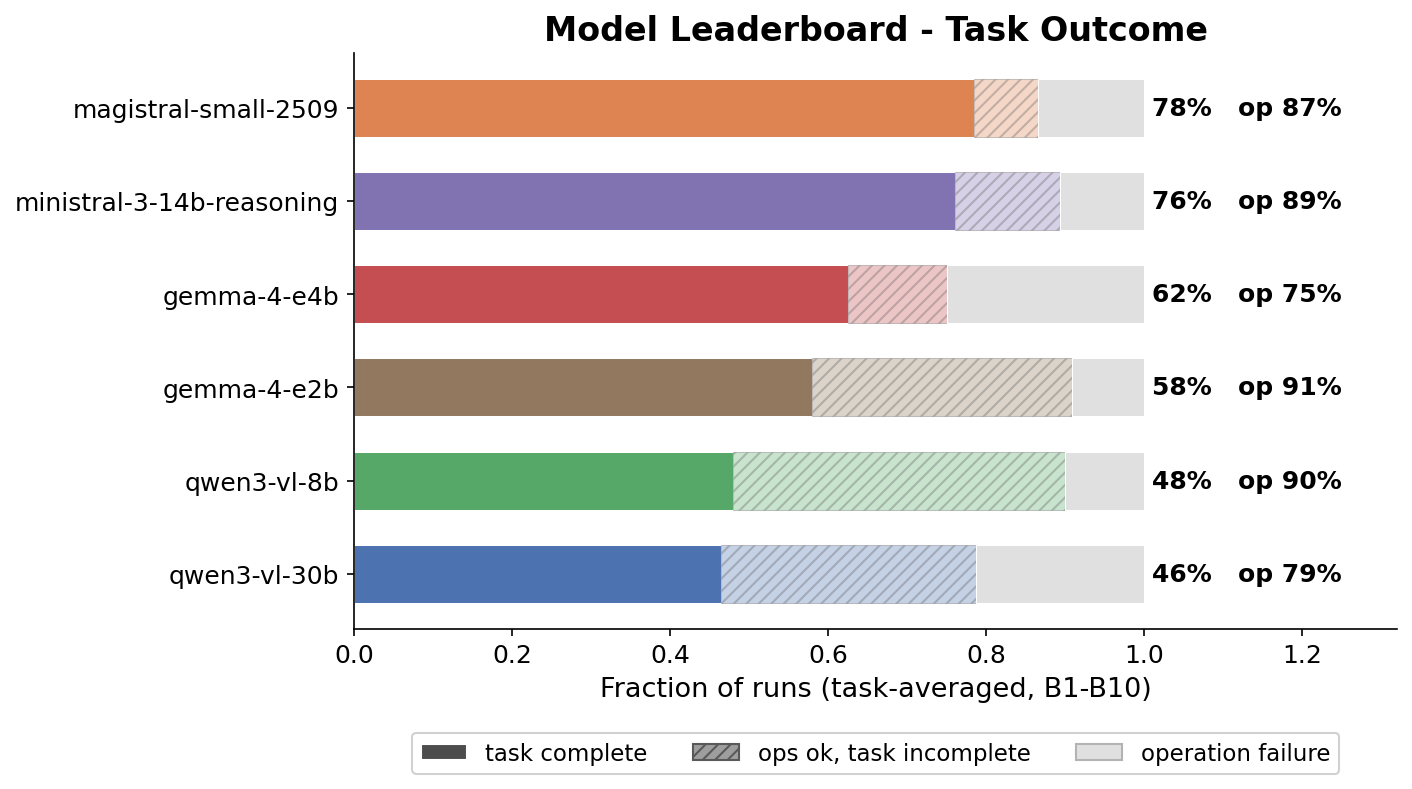
\includegraphics[width=0.9\linewidth]{images/03_model_leaderboard.png}
	\caption{Task-averaged success per model, ranked by task completion. Where a model's operation-level rate runs ahead of its task rate, because it emits trivially short plans that execute but do not finish the task (e.g.\ \gls{qwen38} on B3, B6, and B7), the operation rate is annotated separately to the right of the bar.}
	\label{fig:model_leaderboard}
\end{figure}

\begin{figure}[htbp]
	\centering
	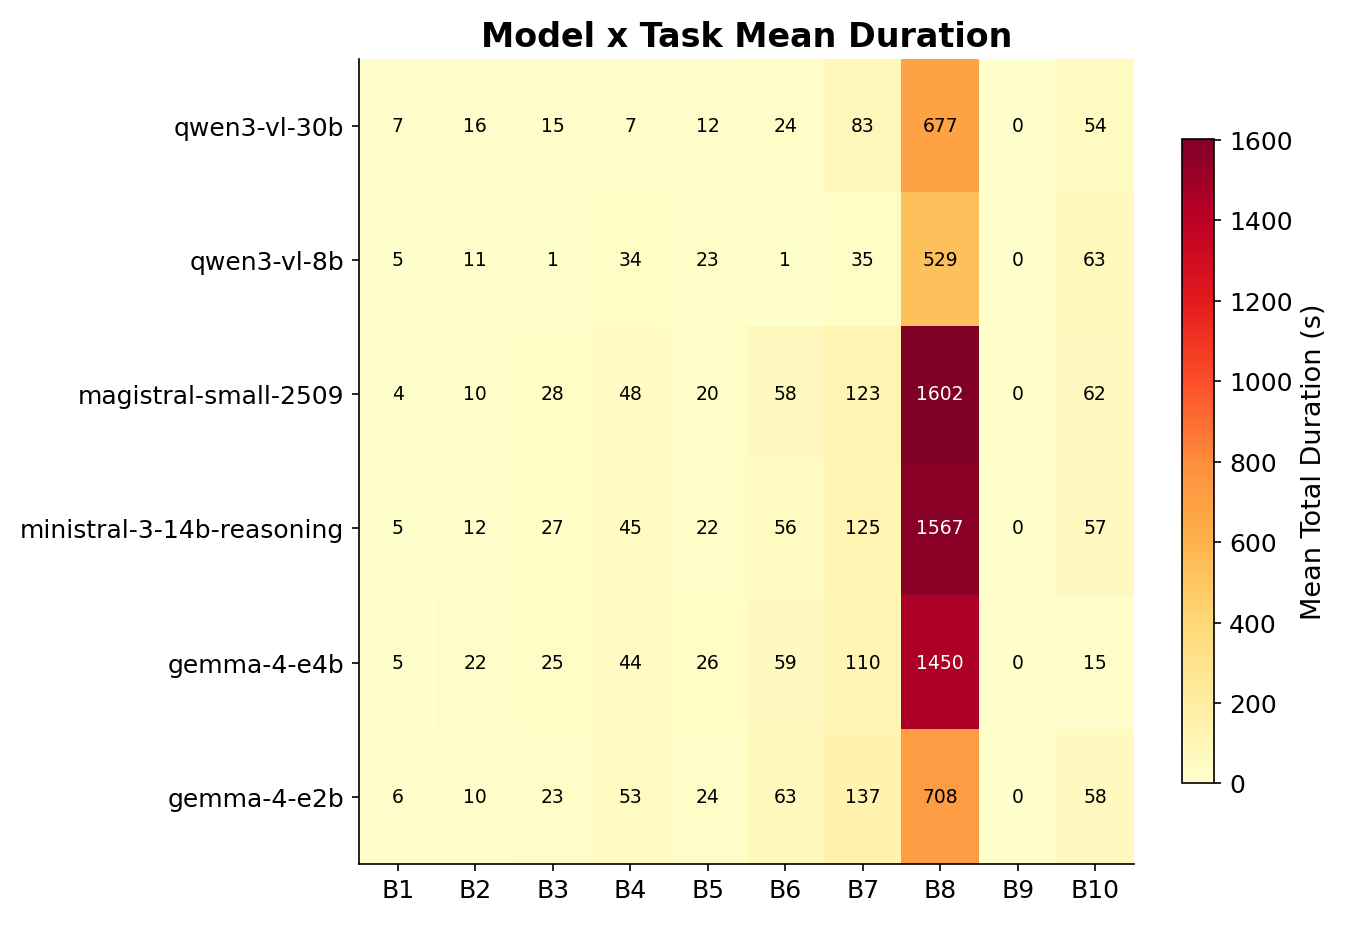
\includegraphics[width=1\linewidth]{images/04_duration_by_model.png}
	\caption{Mean total duration per benchmark and model. B8 dominates by an order of magnitude; the shorter Qwen3 durations on B3--B7 reflect incomplete plans terminating early and not quicker execution.}
	\label{fig:duration_by_model}
\end{figure}

\begingroup
\footnotesize
\setlength{\tabcolsep}{3pt}
\setlength{\extrarowheight}{0pt}
\renewcommand{\arraystretch}{1.0}
\convertXColumns
\begin{tabularx}{\linewidth}{@{}l*{8}{>{\centering\arraybackslash}X}@{}}
	\caption{Detailed overview of all system benchmark runs (B1--B10) for all six models, five runs each (B9 extended to twenty runs per model). The success-rate column is the per-run \texttt{success\_rate} recorded by the harness (operation-level for these single-task benchmarks); task-level outcomes are analyzed in Chapter~\ref{evaluation}. Columns: Succ.\ = per-run success rate; Total = total duration (s); Ops = operations succeeded/executed (for the parse-only B9, Ops counts parsed plan entries, scored failed, rather than dispatched operations); Avg = total duration divided by operations executed, which includes inter-step dispatch overhead; Slowest = slowest step duration (ms); Halluc.\ = hallucinated operations; Reflex.\ = reflection recoveries; Negot.\ = negotiation rounds.}\label{tab:system_benchmark_runs} \\
	\toprule
	\textbf{Task} & \textbf{Succ.} & \textbf{Total}    & \textbf{Ops} & \textbf{Avg}     & \textbf{Slowest} & \textbf{Halluc.} & \textbf{Reflex.} & \textbf{Negot.}                                                                                                                                                                                                                                                                                                                                                                                                                                                                                                                                                                                                                                                                                       \\
	\midrule
	\endfirsthead
	\toprule
	\textbf{Task} & \textbf{Succ.} & \textbf{Total}    & \textbf{Ops} & \textbf{Avg}     & \textbf{Slowest} & \textbf{Halluc.} & \textbf{Reflex.} & \textbf{Negot.}                                                                                                                                                                                                                                                                                                                                                                                                                                                                                                                                                                                                                                                                                       \\
	\midrule
	\endhead
	\midrule
	\multicolumn{9}{r}{\footnotesize Continued on next page}                                                                                                                                                                                                                                                                                                                                                                                                                                                                                                                                                                                                                                                                                                                                                                                              \\
	\endfoot
	\bottomrule
	\endlastfoot
	\multirow{5}{*}{\makecell[l]{\textbf{B1:} \gls{magi} \\ Navigate to Object.}}
	              & 1.000          & 5.16s             & 2/2          & 2579ms           & 4254ms           & 0                & 0                & 0                                                                                                                                                                                                                                                                                                                                                                                                                                                                                                                                                                                                                                                                                                     \\*
	              & 1.000          & 4.27s             & 2/2          & 2137ms           & 3522ms           & 0                & 0                & 0                                                                                                                                                                                                                                                                                                                                                                                                                                                                                                                                                                                                                                                                                                     \\*
	              & 1.000          & 3.83s             & 2/2          & 1913ms           & \textbf{3056ms}  & 0                & 0                & 0                                                                                                                                                                                                                                                                                                                                                                                                                                                                                                                                                                                                                                                                                                     \\*
	              & 1.000          & 5.00s             & 2/2          & 2497ms           & 4240ms           & 0                & 0                & 0                                                                                                                                                                                                                                                                                                                                                                                                                                                                                                                                                                                                                                                                                                     \\*
	              & 1.000          & \textbf{3.82s}    & 2/2          & \textbf{1908ms}  & 3069ms           & 0                & 0                & 0                                                                                                                                                                                                                                                                                                                                                                                                                                                                                                                                                                                                                                                                                                     \\
	\midrule
	\multirow{5}{*}{\makecell[l]{\textbf{B1:} \gls{mini} \\ Navigate to Object.}}
	              & 1.000          & \textbf{3.91s}    & 2/2          & \textbf{1954ms}  & \textbf{3043ms}  & 0                & 0                & 0                                                                                                                                                                                                                                                                                                                                                                                                                                                                                                                                                                                                                                                                                                     \\*
	              & 1.000          & 4.69s             & 2/2          & 2342ms           & 3925ms           & 0                & 0                & 0                                                                                                                                                                                                                                                                                                                                                                                                                                                                                                                                                                                                                                                                                                     \\*
	              & 1.000          & 5.63s             & 2/2          & 2816ms           & 4793ms           & 0                & 0                & 0                                                                                                                                                                                                                                                                                                                                                                                                                                                                                                                                                                                                                                                                                                     \\*
	              & 1.000          & 5.09s             & 2/2          & 2547ms           & 4331ms           & 0                & 0                & 0                                                                                                                                                                                                                                                                                                                                                                                                                                                                                                                                                                                                                                                                                                     \\*
	              & 1.000          & 6.09s             & 2/2          & 3042ms           & 5322ms           & 0                & 0                & 0                                                                                                                                                                                                                                                                                                                                                                                                                                                                                                                                                                                                                                                                                                     \\
	\midrule
	\multirow{5}{*}{\makecell[l]{\textbf{B1:} \gls{qwen38} \\ Navigate to Object.}}
	              & 1.000          & 4.76s             & 2/2          & 2377ms           & 3924ms           & 0                & 0                & 0                                                                                                                                                                                                                                                                                                                                                                                                                                                                                                                                                                                                                                                                                                     \\*
	              & 1.000          & 4.13s             & 2/2          & 2064ms           & 3369ms           & 0                & 0                & 0                                                                                                                                                                                                                                                                                                                                                                                                                                                                                                                                                                                                                                                                                                     \\*
	              & 1.000          & 4.75s             & 2/2          & 2374ms           & 4003ms           & 0                & 0                & 0                                                                                                                                                                                                                                                                                                                                                                                                                                                                                                                                                                                                                                                                                                     \\*
	              & 1.000          & 5.50s             & 2/2          & 2750ms           & 4745ms           & 0                & 0                & 0                                                                                                                                                                                                                                                                                                                                                                                                                                                                                                                                                                                                                                                                                                     \\*
	              & 1.000          & \textbf{3.86s}    & 2/2          & \textbf{1928ms}  & \textbf{3110ms}  & 0                & 0                & 0                                                                                                                                                                                                                                                                                                                                                                                                                                                                                                                                                                                                                                                                                                     \\
	\midrule
	\multirow{5}{*}{\makecell[l]{\textbf{B1:} \gls{qwen330} \\ Navigate to Object.}}
	              & 1.000          & 5.57s             & 2/2          & 2784ms           & 4803ms           & 0                & 0                & 0                                                                                                                                                                                                                                                                                                                                                                                                                                                                                                                                                                                                                                                                                                     \\*
	              & 1.000          & 9.20s             & 2/2          & 4602ms           & 8423ms           & 0                & 0                & 0                                                                                                                                                                                                                                                                                                                                                                                                                                                                                                                                                                                                                                                                                                     \\*
	              & 1.000          & 9.18s             & 2/2          & 4591ms           & 8419ms           & 0                & 0                & 0                                                                                                                                                                                                                                                                                                                                                                                                                                                                                                                                                                                                                                                                                                     \\*
	              & 1.000          & 9.46s             & 2/2          & 4730ms           & 8711ms           & 0                & 0                & 0                                                                                                                                                                                                                                                                                                                                                                                                                                                                                                                                                                                                                                                                                                     \\*
	              & 1.000          & \textbf{3.47s}    & 2/2          & \textbf{1735ms}  & \textbf{2722ms}  & 0                & 0                & 0                                                                                                                                                                                                                                                                                                                                                                                                                                                                                                                                                                                                                                                                                                     \\
	\midrule
	\multirow{5}{*}{\makecell[l]{\textbf{B1:} \gls{gema42} \\ Navigate to Object.}}
	              & 1.000          & 5.87s             & 2/2          & 2936ms           & 5041ms           & 0                & 0                & 0                                                                                                                                                                                                                                                                                                                                                                                                                                                                                                                                                                                                                                                                                                     \\*
	              & 1.000          & 9.39s             & 2/2          & 4694ms           & 8627ms           & 0                & 0                & 0                                                                                                                                                                                                                                                                                                                                                                                                                                                                                                                                                                                                                                                                                                     \\*
	              & 1.000          & 5.47s             & 2/2          & 2734ms           & 4716ms           & 0                & 0                & 0                                                                                                                                                                                                                                                                                                                                                                                                                                                                                                                                                                                                                                                                                                     \\*
	              & 1.000          & \textbf{5.28s}    & 2/2          & \textbf{2640ms}  & \textbf{4528ms}  & 0                & 0                & 0                                                                                                                                                                                                                                                                                                                                                                                                                                                                                                                                                                                                                                                                                                     \\*
	              & 1.000          & 6.05s             & 2/2          & 3025ms           & 5300ms           & 0                & 0                & 0                                                                                                                                                                                                                                                                                                                                                                                                                                                                                                                                                                                                                                                                                                     \\
	\midrule
	\multirow{5}{*}{\makecell[l]{\textbf{B1:} \gls{gema44} \\ Navigate to Object.}}
	              & 1.000          & 5.71s             & 2/2          & 2855ms           & 4855ms           & 0                & 0                & 0                                                                                                                                                                                                                                                                                                                                                                                                                                                                                                                                                                                                                                                                                                     \\*
	              & 1.000          & 5.87s             & 2/2          & 2935ms           & 5118ms           & 0                & 0                & 0                                                                                                                                                                                                                                                                                                                                                                                                                                                                                                                                                                                                                                                                                                     \\*
	              & 1.000          & \textbf{3.62s}    & 2/2          & \textbf{1807ms}  & \textbf{2805ms}  & 0                & 0                & 0                                                                                                                                                                                                                                                                                                                                                                                                                                                                                                                                                                                                                                                                                                     \\*
	              & 1.000          & 5.58s             & 2/2          & 2790ms           & 4729ms           & 0                & 0                & 0                                                                                                                                                                                                                                                                                                                                                                                                                                                                                                                                                                                                                                                                                                     \\*
	              & 1.000          & 5.86s             & 2/2          & 2931ms           & 4975ms           & 0                & 0                & 0                                                                                                                                                                                                                                                                                                                                                                                                                                                                                                                                                                                                                                                                                                     \\
	\midrule[\heavyrulewidth]
	\multirow{5}{*}{\makecell[l]{\textbf{B2:} \gls{magi} \\ Sequential Navigation.}}
	              & 1.000          & 9.61s             & 4/4          & 2402ms           & 4650ms           & 0                & 0                & 0                                                                                                                                                                                                                                                                                                                                                                                                                                                                                                                                                                                                                                                                                                     \\*
	              & 1.000          & \textbf{8.62s}    & 4/4          & \textbf{2155ms}  & \textbf{3803ms}  & 0                & 0                & 0                                                                                                                                                                                                                                                                                                                                                                                                                                                                                                                                                                                                                                                                                                     \\*
	              & 1.000          & 12.46s            & 4/4          & 3114ms           & 6376ms           & 0                & 0                & 0                                                                                                                                                                                                                                                                                                                                                                                                                                                                                                                                                                                                                                                                                                     \\*
	              & 1.000          & 10.28s            & 4/4          & 2571ms           & 4530ms           & 0                & 0                & 0                                                                                                                                                                                                                                                                                                                                                                                                                                                                                                                                                                                                                                                                                                     \\*
	              & 1.000          & 9.09s             & 4/4          & 2273ms           & 4209ms           & 0                & 0                & 0                                                                                                                                                                                                                                                                                                                                                                                                                                                                                                                                                                                                                                                                                                     \\
	\midrule
	\multirow{5}{*}{\makecell[l]{\textbf{B2:} \gls{mini} \\ Sequential Navigation.}}
	              & 1.000          & 14.61s            & 4/4          & 3652ms           & 7813ms           & 0                & 0                & 0                                                                                                                                                                                                                                                                                                                                                                                                                                                                                                                                                                                                                                                                                                     \\*
	              & 1.000          & 14.55s            & 4/4          & 3637ms           & 8349ms           & 0                & 0                & 0                                                                                                                                                                                                                                                                                                                                                                                                                                                                                                                                                                                                                                                                                                     \\*
	              & 1.000          & 10.30s            & 4/4          & 2575ms           & 5946ms           & 0                & 0                & 0                                                                                                                                                                                                                                                                                                                                                                                                                                                                                                                                                                                                                                                                                                     \\*
	              & 1.000          & \textbf{9.54s}    & 4/4          & \textbf{2385ms}  & \textbf{4335ms}  & 0                & 0                & 0                                                                                                                                                                                                                                                                                                                                                                                                                                                                                                                                                                                                                                                                                                     \\*
	              & 1.000          & 10.45s            & 4/4          & 2613ms           & 4803ms           & 0                & 0                & 0                                                                                                                                                                                                                                                                                                                                                                                                                                                                                                                                                                                                                                                                                                     \\
	\midrule
	\multirow{5}{*}{\makecell[l]{\textbf{B2:} \gls{qwen38} \\ Sequential Navigation.}}
	              & 1.000          & 11.39s            & 4/4          & 2847ms           & 6256ms           & 0                & 0                & 0                                                                                                                                                                                                                                                                                                                                                                                                                                                                                                                                                                                                                                                                                                     \\*
	              & 1.000          & 11.34s            & 4/4          & 2834ms           & 4976ms           & 0                & 0                & 0                                                                                                                                                                                                                                                                                                                                                                                                                                                                                                                                                                                                                                                                                                     \\*
	              & 1.000          & 12.37s            & 4/4          & 3091ms           & 5700ms           & 0                & 0                & 0                                                                                                                                                                                                                                                                                                                                                                                                                                                                                                                                                                                                                                                                                                     \\*
	              & 1.000          & 13.35s            & 4/4          & 3338ms           & 7138ms           & 0                & 0                & 0                                                                                                                                                                                                                                                                                                                                                                                                                                                                                                                                                                                                                                                                                                     \\*
	              & 1.000          & \textbf{7.87s}    & 4/4          & \textbf{1968ms}  & \textbf{3216ms}  & 0                & 0                & 0                                                                                                                                                                                                                                                                                                                                                                                                                                                                                                                                                                                                                                                                                                     \\
	\midrule
	\multirow{5}{*}{\makecell[l]{\textbf{B2:} \gls{qwen330} \\ Sequential Navigation.}}
	              & 1.000          & \textbf{9.02s}    & 4/4          & \textbf{2254ms}  & \textbf{4020ms}  & 0                & 0                & 0                                                                                                                                                                                                                                                                                                                                                                                                                                                                                                                                                                                                                                                                                                     \\*
	              & 1.000          & 9.97s             & 4/4          & 2492ms           & 4748ms           & 0                & 0                & 0                                                                                                                                                                                                                                                                                                                                                                                                                                                                                                                                                                                                                                                                                                     \\*
	              & 1.000          & 11.61s            & 4/4          & 2902ms           & 5191ms           & 0                & 0                & 0                                                                                                                                                                                                                                                                                                                                                                                                                                                                                                                                                                                                                                                                                                     \\*
	              & 1.000          & 11.64s            & 4/4          & 2909ms           & 5642ms           & 0                & 0                & 0                                                                                                                                                                                                                                                                                                                                                                                                                                                                                                                                                                                                                                                                                                     \\*
	              & 1.000          & 37.86s            & 4/4          & 9463ms           & 19070ms          & 0                & 0                & 0                                                                                                                                                                                                                                                                                                                                                                                                                                                                                                                                                                                                                                                                                                     \\
	\midrule
	\multirow{5}{*}{\makecell[l]{\textbf{B2:} \gls{gema42} \\ Sequential Navigation.}}
	              & 1.000          & 9.80s             & 4/4          & 2449ms           & 4976ms           & 0                & 0                & 0                                                                                                                                                                                                                                                                                                                                                                                                                                                                                                                                                                                                                                                                                                     \\*
	              & 1.000          & 9.33s             & 4/4          & 2331ms           & \textbf{4019ms}  & 0                & 0                & 0                                                                                                                                                                                                                                                                                                                                                                                                                                                                                                                                                                                                                                                                                                     \\*
	              & 1.000          & 9.75s             & 4/4          & 2437ms           & 4432ms           & 0                & 0                & 0                                                                                                                                                                                                                                                                                                                                                                                                                                                                                                                                                                                                                                                                                                     \\*
	              & 1.000          & 10.59s            & 4/4          & 2646ms           & 4603ms           & 0                & 0                & 0                                                                                                                                                                                                                                                                                                                                                                                                                                                                                                                                                                                                                                                                                                     \\*
	              & 1.000          & \textbf{9.22s}    & 4/4          & \textbf{2304ms}  & 5204ms           & 0                & 0                & 0                                                                                                                                                                                                                                                                                                                                                                                                                                                                                                                                                                                                                                                                                                     \\
	\midrule
	\multirow{5}{*}{\makecell[l]{\textbf{B2:} \gls{gema44} \\ Sequential Navigation.}}
	              & 1.000          & 69.70s            & 4/4          & 17424ms          & 4669ms           & 0                & 0                & 0                                                                                                                                                                                                                                                                                                                                                                                                                                                                                                                                                                                                                                                                                                     \\*
	              & 1.000          & 10.92s            & 4/4          & 2728ms           & 5036ms           & 0                & 0                & 0                                                                                                                                                                                                                                                                                                                                                                                                                                                                                                                                                                                                                                                                                                     \\*
	              & 1.000          & 9.58s             & 4/4          & 2396ms           & 4574ms           & 0                & 0                & 0                                                                                                                                                                                                                                                                                                                                                                                                                                                                                                                                                                                                                                                                                                     \\*
	              & 1.000          & 11.04s            & 4/4          & 2760ms           & 5221ms           & 0                & 0                & 0                                                                                                                                                                                                                                                                                                                                                                                                                                                                                                                                                                                                                                                                                                     \\*
	              & 1.000          & \textbf{9.43s}    & 4/4          & \textbf{2358ms}  & \textbf{4571ms}  & 0                & 0                & 0                                                                                                                                                                                                                                                                                                                                                                                                                                                                                                                                                                                                                                                                                                     \\
	\midrule[\heavyrulewidth]
	\multirow{5}{*}{\makecell[l]{\textbf{B3:} \gls{magi} \\ Navigate and Lift.}}
	              & 1.000          & 25.61s            & 3/3          & 8537ms           & \textbf{15996ms} & 0                & 0                & 0                                                                                                                                                                                                                                                                                                                                                                                                                                                                                                                                                                                                                                                                                                     \\*
	              & 1.000          & 27.22s            & 3/3          & 9074ms           & 18653ms          & 0                & 0                & 0                                                                                                                                                                                                                                                                                                                                                                                                                                                                                                                                                                                                                                                                                                     \\*
	              & 1.000          & 38.84s            & 3/3          & 12948ms          & 29547ms          & 0                & 0                & 0                                                                                                                                                                                                                                                                                                                                                                                                                                                                                                                                                                                                                                                                                                     \\*
	              & 1.000          & 23.62s            & 3/3          & 7872ms           & 17992ms          & 0                & 0                & 0                                                                                                                                                                                                                                                                                                                                                                                                                                                                                                                                                                                                                                                                                                     \\*
	              & 1.000          & \textbf{23.01s}   & 3/3          & \textbf{7669ms}  & 17008ms          & 0                & 0                & 0                                                                                                                                                                                                                                                                                                                                                                                                                                                                                                                                                                                                                                                                                                     \\
	\midrule
	\multirow{5}{*}{\makecell[l]{\textbf{B3:} \gls{mini} \\ Navigate and Lift.}}
	              & 1.000          & 28.00s            & 3/3          & 9333ms           & 19113ms          & 0                & 0                & 0                                                                                                                                                                                                                                                                                                                                                                                                                                                                                                                                                                                                                                                                                                     \\*
	              & 1.000          & 27.74s            & 3/3          & 9245ms           & 19251ms          & 0                & 0                & 0                                                                                                                                                                                                                                                                                                                                                                                                                                                                                                                                                                                                                                                                                                     \\*
	              & 1.000          & \textbf{25.26s}   & 3/3          & \textbf{8421ms}  & \textbf{16322ms} & 0                & 0                & 0                                                                                                                                                                                                                                                                                                                                                                                                                                                                                                                                                                                                                                                                                                     \\*
	              & 1.000          & 27.01s            & 3/3          & 9004ms           & 19173ms          & 0                & 0                & 0                                                                                                                                                                                                                                                                                                                                                                                                                                                                                                                                                                                                                                                                                                     \\*
	              & 1.000          & 29.46s            & 3/3          & 9820ms           & 21877ms          & 0                & 0                & 0                                                                                                                                                                                                                                                                                                                                                                                                                                                                                                                                                                                                                                                                                                     \\
	\midrule
	\multirow{5}{*}{\makecell[l]{\textbf{B3:} \gls{qwen38} \\ Navigate and Lift.}}
	              & 1.000          & 0.75s             & 1/1          & 747ms            & 747ms            & 0                & 0                & 0                                                                                                                                                                                                                                                                                                                                                                                                                                                                                                                                                                                                                                                                                                     \\*
	              & 1.000          & 0.74s             & 1/1          & 744ms            & 744ms            & 0                & 0                & 0                                                                                                                                                                                                                                                                                                                                                                                                                                                                                                                                                                                                                                                                                                     \\*
	              & 1.000          & \textbf{0.74s}    & 1/1          & \textbf{743ms}   & \textbf{743ms}   & 0                & 0                & 0                                                                                                                                                                                                                                                                                                                                                                                                                                                                                                                                                                                                                                                                                                     \\*
	              & 1.000          & 0.75s             & 1/1          & 749ms            & 749ms            & 0                & 0                & 0                                                                                                                                                                                                                                                                                                                                                                                                                                                                                                                                                                                                                                                                                                     \\*
	              & 1.000          & 0.75s             & 1/1          & 749ms            & 749ms            & 0                & 0                & 0                                                                                                                                                                                                                                                                                                                                                                                                                                                                                                                                                                                                                                                                                                     \\
	\midrule
	\multirow{5}{*}{\makecell[l]{\textbf{B3:} \gls{qwen330} \\ Navigate and Lift.}}
	              & 1.000          & 19.70s            & 3/3          & 6566ms           & 13504ms          & 0                & 0                & 0                                                                                                                                                                                                                                                                                                                                                                                                                                                                                                                                                                                                                                                                                                     \\*
	              & 1.000          & 19.23s            & 3/3          & 6409ms           & 13381ms          & 0                & 0                & 0                                                                                                                                                                                                                                                                                                                                                                                                                                                                                                                                                                                                                                                                                                     \\*
	              & 1.000          & 0.00s             & 1/1          & 2ms              & 2ms              & 0                & 0                & 0                                                                                                                                                                                                                                                                                                                                                                                                                                                                                                                                                                                                                                                                                                     \\*
	              & 1.000          & 33.67s            & 3/3          & 11223ms          & 24586ms          & 0                & 0                & 0                                                                                                                                                                                                                                                                                                                                                                                                                                                                                                                                                                                                                                                                                                     \\*
	              & 1.000          & \textbf{0.00s}    & 1/1          & \textbf{1ms}     & \textbf{1ms}     & 0                & 0                & 0                                                                                                                                                                                                                                                                                                                                                                                                                                                                                                                                                                                                                                                                                                     \\
	\midrule
	\multirow{5}{*}{\makecell[l]{\textbf{B3:} \gls{gema42} \\ Navigate and Lift.}}
	              & 1.000          & 20.85s            & 3/3          & 6948ms           & \textbf{12427ms} & 0                & 0                & 0                                                                                                                                                                                                                                                                                                                                                                                                                                                                                                                                                                                                                                                                                                     \\*
	              & 1.000          & 24.73s            & 3/3          & 8242ms           & 17724ms          & 0                & 0                & 0                                                                                                                                                                                                                                                                                                                                                                                                                                                                                                                                                                                                                                                                                                     \\*
	              & 1.000          & \textbf{20.55s}   & 3/3          & \textbf{6851ms}  & 13381ms          & 0                & 0                & 0                                                                                                                                                                                                                                                                                                                                                                                                                                                                                                                                                                                                                                                                                                     \\*
	              & 1.000          & 24.88s            & 3/3          & 8293ms           & 16019ms          & 0                & 0                & 0                                                                                                                                                                                                                                                                                                                                                                                                                                                                                                                                                                                                                                                                                                     \\*
	              & 1.000          & 24.70s            & 3/3          & 8233ms           & 18066ms          & 0                & 0                & 0                                                                                                                                                                                                                                                                                                                                                                                                                                                                                                                                                                                                                                                                                                     \\
	\midrule
	\multirow{5}{*}{\makecell[l]{\textbf{B3:} \gls{gema44} \\ Navigate and Lift.}}
	              & 1.000          & 26.35s            & 3/3          & 8782ms           & 17299ms          & 0                & 0                & 0                                                                                                                                                                                                                                                                                                                                                                                                                                                                                                                                                                                                                                                                                                     \\*
	              & 1.000          & \textbf{20.59s}   & 3/3          & \textbf{6861ms}  & 13558ms          & 0                & 0                & 0                                                                                                                                                                                                                                                                                                                                                                                                                                                                                                                                                                                                                                                                                                     \\*
	              & 1.000          & 23.88s            & 3/3          & 7958ms           & 17442ms          & 0                & 0                & 0                                                                                                                                                                                                                                                                                                                                                                                                                                                                                                                                                                                                                                                                                                     \\*
	              & 1.000          & 21.02s            & 3/3          & 7007ms           & \textbf{13431ms} & 0                & 0                & 0                                                                                                                                                                                                                                                                                                                                                                                                                                                                                                                                                                                                                                                                                                     \\*
	              & 1.000          & 34.08s            & 3/3          & 11361ms          & 28359ms          & 0                & 0                & 0                                                                                                                                                                                                                                                                                                                                                                                                                                                                                                                                                                                                                                                                                                     \\
	\midrule[\heavyrulewidth]
	\multirow{5}{*}{\makecell[l]{\textbf{B4:} \gls{magi} \\ Pick and Place.}}
	              & 1.000          & \textbf{36.77s}   & 4/4          & \textbf{9192ms}  & 24708ms          & 0                & 0                & 0                                                                                                                                                                                                                                                                                                                                                                                                                                                                                                                                                                                                                                                                                                     \\*
	              & 1.000          & 55.12s            & 4/4          & 13780ms          & 39439ms          & 0                & 0                & 0                                                                                                                                                                                                                                                                                                                                                                                                                                                                                                                                                                                                                                                                                                     \\*
	              & 1.000          & 37.51s            & 4/4          & 9376ms           & \textbf{23420ms} & 0                & 0                & 0                                                                                                                                                                                                                                                                                                                                                                                                                                                                                                                                                                                                                                                                                                     \\*
	              & 1.000          & 46.56s            & 4/4          & 11639ms          & 33145ms          & 0                & 0                & 0                                                                                                                                                                                                                                                                                                                                                                                                                                                                                                                                                                                                                                                                                                     \\*
	              & 1.000          & 66.13s            & 4/4          & 16533ms          & 51416ms          & 0                & 0                & 0                                                                                                                                                                                                                                                                                                                                                                                                                                                                                                                                                                                                                                                                                                     \\
	\midrule
	\multirow{5}{*}{\makecell[l]{\textbf{B4:} \gls{mini} \\ Pick and Place.}}
	              & 1.000          & 48.61s            & 4/4          & 12153ms          & 33341ms          & 0                & 0                & 0                                                                                                                                                                                                                                                                                                                                                                                                                                                                                                                                                                                                                                                                                                     \\*
	              & 1.000          & 45.47s            & 4/4          & 11368ms          & 33392ms          & 0                & 0                & 0                                                                                                                                                                                                                                                                                                                                                                                                                                                                                                                                                                                                                                                                                                     \\*
	              & 1.000          & \textbf{35.92s}   & 4/4          & \textbf{8979ms}  & \textbf{23803ms} & 0                & 0                & 0                                                                                                                                                                                                                                                                                                                                                                                                                                                                                                                                                                                                                                                                                                     \\*
	              & 1.000          & 49.06s            & 4/4          & 12264ms          & 35240ms          & 0                & 0                & 0                                                                                                                                                                                                                                                                                                                                                                                                                                                                                                                                                                                                                                                                                                     \\*
	              & 1.000          & 44.42s            & 4/4          & 11105ms          & 28564ms          & 0                & 0                & 0                                                                                                                                                                                                                                                                                                                                                                                                                                                                                                                                                                                                                                                                                                     \\
	\midrule
	\multirow{5}{*}{\makecell[l]{\textbf{B4:} \gls{qwen38} \\ Pick and Place.}}
	              & 1.000          & 48.92s            & 4/4          & 12229ms          & 34251ms          & 0                & 0                & 0                                                                                                                                                                                                                                                                                                                                                                                                                                                                                                                                                                                                                                                                                                     \\*
	              & 1.000          & 38.27s            & 4/4          & 9567ms           & 23152ms          & 0                & 0                & 0                                                                                                                                                                                                                                                                                                                                                                                                                                                                                                                                                                                                                                                                                                     \\*
	              & 1.000          & 35.98s            & 4/4          & 8994ms           & 20616ms          & 0                & 0                & 0                                                                                                                                                                                                                                                                                                                                                                                                                                                                                                                                                                                                                                                                                                     \\*
	              & 1.000          & 47.48s            & 4/4          & 11869ms          & 32689ms          & 0                & 0                & 0                                                                                                                                                                                                                                                                                                                                                                                                                                                                                                                                                                                                                                                                                                     \\*
	              & 1.000          & \textbf{0.74s}    & 1/1          & \textbf{743ms}   & \textbf{743ms}   & 0                & 0                & 0                                                                                                                                                                                                                                                                                                                                                                                                                                                                                                                                                                                                                                                                                                     \\
	\midrule
	\multirow{5}{*}{\makecell[l]{\textbf{B4:} \gls{qwen330} \\ Pick and Place.}}
	              & 1.000          & \textbf{0.00s}    & 1/1          & \textbf{1ms}     & \textbf{1ms}     & 0                & 0                & 0                                                                                                                                                                                                                                                                                                                                                                                                                                                                                                                                                                                                                                                                                                     \\*
	              & 1.000          & 0.00s             & 1/1          & 2ms              & 1ms              & 0                & 0                & 0                                                                                                                                                                                                                                                                                                                                                                                                                                                                                                                                                                                                                                                                                                     \\*
	              & 1.000          & 0.00s             & 1/1          & 2ms              & 2ms              & 0                & 0                & 0                                                                                                                                                                                                                                                                                                                                                                                                                                                                                                                                                                                                                                                                                                     \\*
	              & 1.000          & 0.00s             & 1/1          & 1ms              & 1ms              & 0                & 0                & 0                                                                                                                                                                                                                                                                                                                                                                                                                                                                                                                                                                                                                                                                                                     \\*
	              & 1.000          & 36.34s            & 4/4          & 9086ms           & 24384ms          & 0                & 0                & 0                                                                                                                                                                                                                                                                                                                                                                                                                                                                                                                                                                                                                                                                                                     \\
	\midrule
	\multirow{5}{*}{\makecell[l]{\textbf{B4:} \gls{gema42} \\ Pick and Place.}}
	              & 1.000          & 47.76s            & 4/4          & 11940ms          & 33712ms          & 0                & 0                & 0                                                                                                                                                                                                                                                                                                                                                                                                                                                                                                                                                                                                                                                                                                     \\*
	              & 1.000          & 65.44s            & 4/4          & 16359ms          & 49747ms          & 0                & 0                & 0                                                                                                                                                                                                                                                                                                                                                                                                                                                                                                                                                                                                                                                                                                     \\*
	              & 1.000          & 72.04s            & 4/4          & 18008ms          & 57813ms          & 0                & 0                & 0                                                                                                                                                                                                                                                                                                                                                                                                                                                                                                                                                                                                                                                                                                     \\*
	              & 1.000          & 47.54s            & 4/4          & 11884ms          & 34512ms          & 0                & 0                & 0                                                                                                                                                                                                                                                                                                                                                                                                                                                                                                                                                                                                                                                                                                     \\*
	              & 1.000          & \textbf{34.29s}   & 4/4          & \textbf{8573ms}  & \textbf{19664ms} & 0                & 0                & 0                                                                                                                                                                                                                                                                                                                                                                                                                                                                                                                                                                                                                                                                                                     \\
	\midrule
	\multirow{5}{*}{\makecell[l]{\textbf{B4:} \gls{gema44} \\ Pick and Place.}}
	              & 1.000          & 37.14s            & 4/4          & 9285ms           & 20344ms          & 0                & 0                & 0                                                                                                                                                                                                                                                                                                                                                                                                                                                                                                                                                                                                                                                                                                     \\*
	              & 1.000          & 57.82s            & 4/4          & 14454ms          & 41752ms          & 0                & 0                & 0                                                                                                                                                                                                                                                                                                                                                                                                                                                                                                                                                                                                                                                                                                     \\*
	              & 1.000          & \textbf{35.59s}   & 4/4          & \textbf{8896ms}  & \textbf{19825ms} & 0                & 0                & 0                                                                                                                                                                                                                                                                                                                                                                                                                                                                                                                                                                                                                                                                                                     \\*
	              & 1.000          & 51.00s            & 4/4          & 12751ms          & 36543ms          & 0                & 0                & 0                                                                                                                                                                                                                                                                                                                                                                                                                                                                                                                                                                                                                                                                                                     \\*
	              & 1.000          & 39.66s            & 4/4          & 9913ms           & 24427ms          & 0                & 0                & 0                                                                                                                                                                                                                                                                                                                                                                                                                                                                                                                                                                                                                                                                                                     \\
	\midrule[\heavyrulewidth]
	\multirow{5}{*}{\makecell[l]{\textbf{B5:} \gls{magi} \\ Pose-Aware Grasp.}}
	              & 1.000          & 13.38s            & 2/2          & 6690ms           & 11051ms          & 0                & 0                & 0                                                                                                                                                                                                                                                                                                                                                                                                                                                                                                                                                                                                                                                                                                     \\*
	              & 1.000          & \textbf{12.83s}   & 2/2          & \textbf{6414ms}  & \textbf{10527ms} & 0                & 0                & 0                                                                                                                                                                                                                                                                                                                                                                                                                                                                                                                                                                                                                                                                                                     \\*
	              & 1.000          & 25.72s            & 2/2          & 12860ms          & 23429ms          & 0                & 0                & 0                                                                                                                                                                                                                                                                                                                                                                                                                                                                                                                                                                                                                                                                                                     \\*
	              & 1.000          & 25.08s            & 2/2          & 12539ms          & 22789ms          & 0                & 0                & 0                                                                                                                                                                                                                                                                                                                                                                                                                                                                                                                                                                                                                                                                                                     \\*
	              & 1.000          & 23.01s            & 2/2          & 11504ms          & 20723ms          & 0                & 0                & 0                                                                                                                                                                                                                                                                                                                                                                                                                                                                                                                                                                                                                                                                                                     \\
	\midrule
	\multirow{5}{*}{\makecell[l]{\textbf{B5:} \gls{mini} \\ Pose-Aware Grasp.}}
	              & 1.000          & 24.44s            & 2/2          & 12219ms          & 21985ms          & 0                & 0                & 0                                                                                                                                                                                                                                                                                                                                                                                                                                                                                                                                                                                                                                                                                                     \\*
	              & 1.000          & 25.15s            & 2/2          & 12574ms          & 22830ms          & 0                & 0                & 0                                                                                                                                                                                                                                                                                                                                                                                                                                                                                                                                                                                                                                                                                                     \\*
	              & 1.000          & \textbf{12.15s}   & 2/2          & \textbf{6076ms}  & \textbf{9856ms}  & 0                & 0                & 0                                                                                                                                                                                                                                                                                                                                                                                                                                                                                                                                                                                                                                                                                                     \\*
	              & 1.000          & 24.00s            & 2/2          & 12000ms          & 21717ms          & 0                & 0                & 0                                                                                                                                                                                                                                                                                                                                                                                                                                                                                                                                                                                                                                                                                                     \\*
	              & 1.000          & 25.92s            & 2/2          & 12959ms          & 23631ms          & 0                & 0                & 0                                                                                                                                                                                                                                                                                                                                                                                                                                                                                                                                                                                                                                                                                                     \\
	\midrule
	\multirow{5}{*}{\makecell[l]{\textbf{B5:} \gls{qwen38} \\ Pose-Aware Grasp.}}
	              & 1.000          & 27.48s            & 2/2          & 13738ms          & 25121ms          & 0                & 0                & 0                                                                                                                                                                                                                                                                                                                                                                                                                                                                                                                                                                                                                                                                                                     \\*
	              & 1.000          & 25.04s            & 2/2          & 12517ms          & 22780ms          & 0                & 0                & 0                                                                                                                                                                                                                                                                                                                                                                                                                                                                                                                                                                                                                                                                                                     \\*
	              & 1.000          & 27.20s            & 2/2          & 13597ms          & 24897ms          & 0                & 0                & 0                                                                                                                                                                                                                                                                                                                                                                                                                                                                                                                                                                                                                                                                                                     \\*
	              & 1.000          & 25.26s            & 2/2          & 12629ms          & 22955ms          & 0                & 0                & 0                                                                                                                                                                                                                                                                                                                                                                                                                                                                                                                                                                                                                                                                                                     \\*
	              & 1.000          & \textbf{12.11s}   & 2/2          & \textbf{6056ms}  & \textbf{9814ms}  & 0                & 0                & 0                                                                                                                                                                                                                                                                                                                                                                                                                                                                                                                                                                                                                                                                                                     \\
	\midrule
	\multirow{5}{*}{\makecell[l]{\textbf{B5:} \gls{qwen330} \\ Pose-Aware Grasp.}}
	              & 1.000          & 15.36s            & 2/2          & 7680ms           & 13066ms          & 0                & 0                & 0                                                                                                                                                                                                                                                                                                                                                                                                                                                                                                                                                                                                                                                                                                     \\*
	              & 1.000          & 24.68s            & 2/2          & 12340ms          & 22410ms          & 0                & 0                & 0                                                                                                                                                                                                                                                                                                                                                                                                                                                                                                                                                                                                                                                                                                     \\*
	              & 1.000          & \textbf{0.00s}    & 1/1          & \textbf{2ms}     & \textbf{1ms}     & 0                & 0                & 0                                                                                                                                                                                                                                                                                                                                                                                                                                                                                                                                                                                                                                                                                                     \\*
	              & 1.000          & 19.05s            & 2/2          & 9523ms           & 16745ms          & 0                & 0                & 0                                                                                                                                                                                                                                                                                                                                                                                                                                                                                                                                                                                                                                                                                                     \\*
	              & 1.000          & 0.00s             & 1/1          & 2ms              & 2ms              & 0                & 0                & 0                                                                                                                                                                                                                                                                                                                                                                                                                                                                                                                                                                                                                                                                                                     \\
	\midrule
	\multirow{5}{*}{\makecell[l]{\textbf{B5:} \gls{gema42} \\ Pose-Aware Grasp.}}
	              & 1.000          & 24.23s            & 2/2          & 12116ms          & 21964ms          & 0                & 0                & 0                                                                                                                                                                                                                                                                                                                                                                                                                                                                                                                                                                                                                                                                                                     \\*
	              & 1.000          & 25.27s            & 2/2          & 12634ms          & 23003ms          & 0                & 0                & 0                                                                                                                                                                                                                                                                                                                                                                                                                                                                                                                                                                                                                                                                                                     \\*
	              & 1.000          & \textbf{11.90s}   & 2/2          & \textbf{5948ms}  & \textbf{9601ms}  & 0                & 0                & 0                                                                                                                                                                                                                                                                                                                                                                                                                                                                                                                                                                                                                                                                                                     \\*
	              & 1.000          & 34.94s            & 2/2          & 17467ms          & 32620ms          & 0                & 0                & 0                                                                                                                                                                                                                                                                                                                                                                                                                                                                                                                                                                                                                                                                                                     \\*
	              & 1.000          & 24.38s            & 2/2          & 12191ms          & 22085ms          & 0                & 0                & 0                                                                                                                                                                                                                                                                                                                                                                                                                                                                                                                                                                                                                                                                                                     \\
	\midrule
	\multirow{5}{*}{\makecell[l]{\textbf{B5:} \gls{gema44} \\ Pose-Aware Grasp.}}
	              & 1.000          & 25.25s            & 2/2          & 12627ms          & 22922ms          & 0                & 0                & 0                                                                                                                                                                                                                                                                                                                                                                                                                                                                                                                                                                                                                                                                                                     \\*
	              & 1.000          & \textbf{25.16s}   & 2/2          & \textbf{12579ms} & \textbf{22788ms} & 0                & 0                & 0                                                                                                                                                                                                                                                                                                                                                                                                                                                                                                                                                                                                                                                                                                     \\*
	              & 1.000          & 26.46s            & 2/2          & 13228ms          & 24131ms          & 0                & 0                & 0                                                                                                                                                                                                                                                                                                                                                                                                                                                                                                                                                                                                                                                                                                     \\*
	              & 1.000          & 28.67s            & 2/2          & 14335ms          & 26334ms          & 0                & 0                & 0                                                                                                                                                                                                                                                                                                                                                                                                                                                                                                                                                                                                                                                                                                     \\*
	              & 1.000          & 25.63s            & 2/2          & 12814ms          & 23134ms          & 0                & 0                & 0                                                                                                                                                                                                                                                                                                                                                                                                                                                                                                                                                                                                                                                                                                     \\
	\midrule[\heavyrulewidth]
	\multirow{5}{*}{\makecell[l]{\textbf{B6:} \gls{magi} \\ Robot Handoff.}}
	              & 1.000          & 50.32s            & 9/9          & 5591ms           & 15720ms          & 0                & 0                & 0                                                                                                                                                                                                                                                                                                                                                                                                                                                                                                                                                                                                                                                                                                     \\*
	              & 1.000          & 82.84s            & 9/9          & 9204ms           & 15677ms          & 0                & 0                & 0                                                                                                                                                                                                                                                                                                                                                                                                                                                                                                                                                                                                                                                                                                     \\*
	              & 1.000          & 66.37s            & 9/9          & 7374ms           & 11590ms          & 0                & 0                & 0                                                                                                                                                                                                                                                                                                                                                                                                                                                                                                                                                                                                                                                                                                     \\*
	              & 1.000          & 48.52s            & 11/11        & \textbf{4411ms}  & \textbf{11064ms} & 0                & 0                & 0                                                                                                                                                                                                                                                                                                                                                                                                                                                                                                                                                                                                                                                                                                     \\*
	              & 1.000          & \textbf{43.28s}   & 9/9          & 4808ms           & 15724ms          & 0                & 0                & 0                                                                                                                                                                                                                                                                                                                                                                                                                                                                                                                                                                                                                                                                                                     \\
	\midrule
	\multirow{5}{*}{\makecell[l]{\textbf{B6:} \gls{mini} \\ Robot Handoff.}}
	              & 1.000          & 60.59s            & 10/10        & 6058ms           & 13926ms          & 0                & 0                & 0                                                                                                                                                                                                                                                                                                                                                                                                                                                                                                                                                                                                                                                                                                     \\*
	              & 1.000          & \textbf{41.55s}   & 9/9          & \textbf{4616ms}  & 13744ms          & 0                & 0                & 0                                                                                                                                                                                                                                                                                                                                                                                                                                                                                                                                                                                                                                                                                                     \\*
	              & 1.000          & 71.75s            & 9/9          & 7972ms           & 39774ms          & 0                & 0                & 0                                                                                                                                                                                                                                                                                                                                                                                                                                                                                                                                                                                                                                                                                                     \\*
	              & 1.000          & 45.54s            & 9/9          & 5060ms           & \textbf{12473ms} & 0                & 0                & 0                                                                                                                                                                                                                                                                                                                                                                                                                                                                                                                                                                                                                                                                                                     \\*
	              & 1.000          & 61.46s            & 8/8          & 7682ms           & 18250ms          & 0                & 0                & 0                                                                                                                                                                                                                                                                                                                                                                                                                                                                                                                                                                                                                                                                                                     \\
	\midrule
	\multirow{5}{*}{\makecell[l]{\textbf{B6:} \gls{qwen38} \\ Robot Handoff.}}
	              & 1.000          & 0.75s             & 1/1          & 749ms            & 749ms            & 0                & 0                & 0                                                                                                                                                                                                                                                                                                                                                                                                                                                                                                                                                                                                                                                                                                     \\*
	              & 1.000          & \textbf{0.74s}    & 1/1          & \textbf{740ms}   & \textbf{740ms}   & 0                & 0                & 0                                                                                                                                                                                                                                                                                                                                                                                                                                                                                                                                                                                                                                                                                                     \\*
	              & 1.000          & 0.75s             & 1/1          & 749ms            & 749ms            & 0                & 0                & 0                                                                                                                                                                                                                                                                                                                                                                                                                                                                                                                                                                                                                                                                                                     \\*
	              & 1.000          & 0.75s             & 1/1          & 750ms            & 749ms            & 0                & 0                & 0                                                                                                                                                                                                                                                                                                                                                                                                                                                                                                                                                                                                                                                                                                     \\*
	              & 1.000          & 0.75s             & 1/1          & 748ms            & 748ms            & 0                & 0                & 0                                                                                                                                                                                                                                                                                                                                                                                                                                                                                                                                                                                                                                                                                                     \\
	\midrule
	\multirow{5}{*}{\makecell[l]{\textbf{B6:} \gls{qwen330} \\ Robot Handoff.}}
	              & 0.800          & 42.70s            & 4/5          & 8539ms           & \textbf{16492ms} & 0                & 0                & 0                                                                                                                                                                                                                                                                                                                                                                                                                                                                                                                                                                                                                                                                                                     \\*
	              & 0.000          & \textbf{8.97s}    & 0/0          & 0ms              & 0ms              & 0                & 0                & 0                                                                                                                                                                                                                                                                                                                                                                                                                                                                                                                                                                                                                                                                                                     \\*
	              & 0.000          & 8.98s             & 0/0          & 0ms              & 0ms              & 0                & 0                & 0                                                                                                                                                                                                                                                                                                                                                                                                                                                                                                                                                                                                                                                                                                     \\*
	              & 0.000          & 9.14s             & 0/0          & 0ms              & 0ms              & 0                & 0                & 0                                                                                                                                                                                                                                                                                                                                                                                                                                                                                                                                                                                                                                                                                                     \\*
	              & 0.364          & 50.35s            & 4/11         & \textbf{4577ms}  & 22634ms          & 0                & 0                & 0                                                                                                                                                                                                                                                                                                                                                                                                                                                                                                                                                                                                                                                                                                     \\
	\midrule
	\multirow{5}{*}{\makecell[l]{\textbf{B6:} \gls{gema42} \\ Robot Handoff.}}
	              & 0.000          & \textbf{26.22s}   & 0/0          & 0ms              & 0ms              & 0                & 0                & 0                                                                                                                                                                                                                                                                                                                                                                                                                                                                                                                                                                                                                                                                                                     \\*
	              & 1.000          & 76.50s            & 11/11        & 6954ms           & 23433ms          & 0                & 0                & 0                                                                                                                                                                                                                                                                                                                                                                                                                                                                                                                                                                                                                                                                                                     \\*
	              & 1.000          & 80.92s            & 14/14        & 5780ms           & 48072ms          & 0                & 0                & 0                                                                                                                                                                                                                                                                                                                                                                                                                                                                                                                                                                                                                                                                                                     \\*
	              & 0.714          & 51.29s            & 10/14        & \textbf{3663ms}  & 51290ms          & 0                & 0                & 0                                                                                                                                                                                                                                                                                                                                                                                                                                                                                                                                                                                                                                                                                                     \\*
	              & 1.000          & 79.03s            & 14/14        & 5645ms           & \textbf{18004ms} & 0                & 0                & 0                                                                                                                                                                                                                                                                                                                                                                                                                                                                                                                                                                                                                                                                                                     \\
	\midrule
	\multirow{5}{*}{\makecell[l]{\textbf{B6:} \gls{gema44} \\ Robot Handoff.}}
	              & 1.000          & 54.83s            & 10/10        & 5482ms           & \textbf{24252ms} & 0                & 0                & 0                                                                                                                                                                                                                                                                                                                                                                                                                                                                                                                                                                                                                                                                                                     \\*
	              & 1.000          & 67.55s            & 9/9          & 7505ms           & 40687ms          & 0                & 0                & 0                                                                                                                                                                                                                                                                                                                                                                                                                                                                                                                                                                                                                                                                                                     \\*
	              & 0.000          & 51.75s            & 0/0          & 0ms              & 0ms              & 0                & 0                & 0                                                                                                                                                                                                                                                                                                                                                                                                                                                                                                                                                                                                                                                                                                     \\*
	              & 0.800          & \textbf{30.22s}   & 8/10         & \textbf{3021ms}  & 26167ms          & 0                & 0                & 0                                                                                                                                                                                                                                                                                                                                                                                                                                                                                                                                                                                                                                                                                                     \\*
	              & 1.000          & 89.32s            & 10/10        & 8931ms           & 48417ms          & 0                & 0                & 0                                                                                                                                                                                                                                                                                                                                                                                                                                                                                                                                                                                                                                                                                                     \\
	\midrule[\heavyrulewidth]
	\multirow{5}{*}{\makecell[l]{\textbf{B7:} \gls{magi} \\ Dual-Robot Reorient.}}
	              & 0.500          & 111.17s           & 4/8          & 13896ms          & 60000ms          & 0                & 0                & 0                                                                                                                                                                                                                                                                                                                                                                                                                                                                                                                                                                                                                                                                                                     \\*
	              & 0.400          & \textbf{43.30s}   & 4/10         & \textbf{4329ms}  & 33596ms          & 0                & 0                & 0                                                                                                                                                                                                                                                                                                                                                                                                                                                                                                                                                                                                                                                                                                     \\*
	              & 0.857          & 210.53s           & 6/7          & 30075ms          & 86544ms          & 0                & 0                & 0                                                                                                                                                                                                                                                                                                                                                                                                                                                                                                                                                                                                                                                                                                     \\*
	              & 0.857          & 206.18s           & 6/7          & 29454ms          & 60675ms          & 0                & 0                & 0                                                                                                                                                                                                                                                                                                                                                                                                                                                                                                                                                                                                                                                                                                     \\*
	              & 0.400          & 46.10s            & 4/10         & 4609ms           & \textbf{32636ms} & 0                & 0                & 0                                                                                                                                                                                                                                                                                                                                                                                                                                                                                                                                                                                                                                                                                                     \\
	\midrule
	\multirow{5}{*}{\makecell[l]{\textbf{B7:} \gls{mini} \\ Dual-Robot Reorient.}}
	              & 0.900          & 192.69s           & 9/10         & 19269ms          & \textbf{15271ms} & 0                & 0                & 0                                                                                                                                                                                                                                                                                                                                                                                                                                                                                                                                                                                                                                                                                                     \\*
	              & 1.000          & 135.12s           & 11/11        & 12283ms          & 23494ms          & 0                & 0                & 0                                                                                                                                                                                                                                                                                                                                                                                                                                                                                                                                                                                                                                                                                                     \\*
	              & 0.875          & 97.75s            & 7/8          & 12218ms          & 63935ms          & 0                & 0                & 0                                                                                                                                                                                                                                                                                                                                                                                                                                                                                                                                                                                                                                                                                                     \\*
	              & 0.900          & \textbf{89.89s}   & 9/10         & \textbf{8989ms}  & 67525ms          & 0                & 0                & 0                                                                                                                                                                                                                                                                                                                                                                                                                                                                                                                                                                                                                                                                                                     \\*
	              & 1.000          & 108.75s           & 8/8          & 13593ms          & 66381ms          & 0                & 0                & 0                                                                                                                                                                                                                                                                                                                                                                                                                                                                                                                                                                                                                                                                                                     \\
	\midrule
	\multirow{5}{*}{\makecell[l]{\textbf{B7:} \gls{qwen38} \\ Dual-Robot Reorient.}}
	              & 1.000          & 80.72s            & 6/6          & 13453ms          & 51451ms          & 0                & 0                & 0                                                                                                                                                                                                                                                                                                                                                                                                                                                                                                                                                                                                                                                                                                     \\*
	              & 1.000          & 0.76s             & 1/1          & 758ms            & 757ms            & 0                & 0                & 0                                                                                                                                                                                                                                                                                                                                                                                                                                                                                                                                                                                                                                                                                                     \\*
	              & 1.000          & 0.74s             & 1/1          & 744ms            & 744ms            & 0                & 0                & 0                                                                                                                                                                                                                                                                                                                                                                                                                                                                                                                                                                                                                                                                                                     \\*
	              & 1.000          & \textbf{0.74s}    & 1/1          & \textbf{741ms}   & \textbf{741ms}   & 0                & 0                & 0                                                                                                                                                                                                                                                                                                                                                                                                                                                                                                                                                                                                                                                                                                     \\*
	              & 1.000          & 90.18s            & 6/6          & 15029ms          & 64198ms          & 0                & 0                & 0                                                                                                                                                                                                                                                                                                                                                                                                                                                                                                                                                                                                                                                                                                     \\
	\midrule
	\multirow{5}{*}{\makecell[l]{\textbf{B7:} \gls{qwen330} \\ Dual-Robot Reorient.}}
	              & 0.750          & 35.94s            & 3/4          & 8984ms           & 30185ms          & 0                & 0                & 0                                                                                                                                                                                                                                                                                                                                                                                                                                                                                                                                                                                                                                                                                                     \\*
	              & 1.000          & 236.77s           & 6/6          & 39461ms          & 23479ms          & 0                & 0                & 0                                                                                                                                                                                                                                                                                                                                                                                                                                                                                                                                                                                                                                                                                                     \\*
	              & 0.125          & \textbf{0.85s}    & 1/8          & \textbf{106ms}   & \textbf{850ms}   & 0                & 0                & 0                                                                                                                                                                                                                                                                                                                                                                                                                                                                                                                                                                                                                                                                                                     \\*
	              & 0.500          & 125.78s           & 3/6          & 20962ms          & 120000ms         & 0                & 0                & 0                                                                                                                                                                                                                                                                                                                                                                                                                                                                                                                                                                                                                                                                                                     \\*
	              & 0.667          & 16.44s            & 2/3          & 5479ms           & 14145ms          & 0                & 0                & 0                                                                                                                                                                                                                                                                                                                                                                                                                                                                                                                                                                                                                                                                                                     \\
	\midrule
	\multirow{5}{*}{\makecell[l]{\textbf{B7:} \gls{gema42} \\ Dual-Robot Reorient.}}
	              & 1.000          & \textbf{32.15s}   & 1/1          & 32151ms          & 11576ms          & 0                & 0                & 0                                                                                                                                                                                                                                                                                                                                                                                                                                                                                                                                                                                                                                                                                                     \\*
	              & 0.000          & 46.25s            & 0/1          & 46246ms          & \textbf{0ms}     & 0                & 0                & 0                                                                                                                                                                                                                                                                                                                                                                                                                                                                                                                                                                                                                                                                                                     \\*
	              & 0.750          & 287.65s           & 3/4          & 71912ms          & 20091ms          & 0                & 0                & 0                                                                                                                                                                                                                                                                                                                                                                                                                                                                                                                                                                                                                                                                                                     \\*
	              & 0.500          & 209.74s           & 1/2          & 104870ms         & 160215ms         & 0                & 0                & 0                                                                                                                                                                                                                                                                                                                                                                                                                                                                                                                                                                                                                                                                                                     \\*
	              & 0.750          & 109.18s           & 3/4          & \textbf{27293ms} & 35947ms          & 0                & 0                & 0                                                                                                                                                                                                                                                                                                                                                                                                                                                                                                                                                                                                                                                                                                     \\
	\midrule
	\multirow{5}{*}{\makecell[l]{\textbf{B7:} \gls{gema44} \\ Dual-Robot Reorient.}}
	              & 1.000          & 86.08s            & 5/5          & \textbf{17216ms} & \textbf{63319ms} & 0                & 0                & 0                                                                                                                                                                                                                                                                                                                                                                                                                                                                                                                                                                                                                                                                                                     \\*
	              & 0.400          & 137.60s           & 2/5          & 27519ms          & 120000ms         & 0                & 0                & 0                                                                                                                                                                                                                                                                                                                                                                                                                                                                                                                                                                                                                                                                                                     \\*
	              & 0.800          & 122.15s           & 4/5          & 24429ms          & 67634ms          & 0                & 0                & 0                                                                                                                                                                                                                                                                                                                                                                                                                                                                                                                                                                                                                                                                                                     \\*
	              & 0.000          & \textbf{67.53s}   & 0/0          & 0ms              & 0ms              & 0                & 0                & 0                                                                                                                                                                                                                                                                                                                                                                                                                                                                                                                                                                                                                                                                                                     \\*
	              & 0.400          & 136.26s           & 2/5          & 27252ms          & 120000ms         & 0                & 0                & 0                                                                                                                                                                                                                                                                                                                                                                                                                                                                                                                                                                                                                                                                                                     \\
	\midrule[\heavyrulewidth]
	\multirow{5}{*}{\makecell[l]{\textbf{B8:} \gls{magi} \\ Heterogeneous Chain.}}
	              & 1.000          & 1698.81s          & 85/85        & 19986ms          & 87476ms          & 0                & 0                & 0                                                                                                                                                                                                                                                                                                                                                                                                                                                                                                                                                                                                                                                                                                     \\*
	              & 1.000          & 1574.63s          & 85/85        & 18525ms          & 87977ms          & 0                & 0                & 0                                                                                                                                                                                                                                                                                                                                                                                                                                                                                                                                                                                                                                                                                                     \\*
	              & 1.000          & 1595.48s          & 85/85        & 18770ms          & \textbf{78550ms} & 0                & 0                & 0                                                                                                                                                                                                                                                                                                                                                                                                                                                                                                                                                                                                                                                                                                     \\*
	              & 1.000          & 1616.27s          & 85/85        & 19014ms          & 80073ms          & 0                & 0                & 0                                                                                                                                                                                                                                                                                                                                                                                                                                                                                                                                                                                                                                                                                                     \\*
	              & 1.000          & \textbf{1526.92s} & 85/85        & \textbf{17963ms} & 84306ms          & 0                & 0                & 0                                                                                                                                                                                                                                                                                                                                                                                                                                                                                                                                                                                                                                                                                                     \\
	\midrule
	\multirow{5}{*}{\makecell[l]{\textbf{B8:} \gls{mini} \\ Heterogeneous Chain.}}
	              & 1.000          & 1761.72s          & 85/85        & 20726ms          & \textbf{82627ms} & 0                & 0                & 0                                                                                                                                                                                                                                                                                                                                                                                                                                                                                                                                                                                                                                                                                                     \\*
	              & 1.000          & 1661.76s          & 85/85        & 19550ms          & 82868ms          & 0                & 0                & 0                                                                                                                                                                                                                                                                                                                                                                                                                                                                                                                                                                                                                                                                                                     \\*
	              & 1.000          & 1432.83s          & 85/85        & \textbf{16856ms} & 82999ms          & 0                & 0                & 0                                                                                                                                                                                                                                                                                                                                                                                                                                                                                                                                                                                                                                                                                                     \\*
	              & 1.000          & 1678.73s          & 85/85        & 19749ms          & 82728ms          & 0                & 0                & 0                                                                                                                                                                                                                                                                                                                                                                                                                                                                                                                                                                                                                                                                                                     \\*
	              & 1.000          & \textbf{1300.98s} & 77/77        & 16895ms          & 84142ms          & 0                & 0                & 0                                                                                                                                                                                                                                                                                                                                                                                                                                                                                                                                                                                                                                                                                                     \\
	\midrule
	\multirow{5}{*}{\makecell[l]{\textbf{B8:} \gls{qwen38} \\ Heterogeneous Chain.}}
	              & 1.000          & \textbf{203.71s}  & 37/37        & \textbf{5505ms}  & \textbf{42928ms} & 0                & 0                & 0                                                                                                                                                                                                                                                                                                                                                                                                                                                                                                                                                                                                                                                                                                     \\*
	              & 1.000          & 643.96s           & 53/53        & 12150ms          & 78160ms          & 0                & 0                & 0                                                                                                                                                                                                                                                                                                                                                                                                                                                                                                                                                                                                                                                                                                     \\*
	              & 1.000          & 441.57s           & 45/45        & 9812ms           & 65194ms          & 0                & 0                & 0                                                                                                                                                                                                                                                                                                                                                                                                                                                                                                                                                                                                                                                                                                     \\*
	              & 1.000          & 679.00s           & 53/53        & 12811ms          & 79056ms          & 0                & 0                & 0                                                                                                                                                                                                                                                                                                                                                                                                                                                                                                                                                                                                                                                                                                     \\*
	              & 0.950          & 675.91s           & 52/53        & 12752ms          & 82685ms          & 0                & 0                & 0                                                                                                                                                                                                                                                                                                                                                                                                                                                                                                                                                                                                                                                                                                     \\
	\midrule
	\multirow{5}{*}{\makecell[l]{\textbf{B8:} \gls{qwen330} \\ Heterogeneous Chain.}}
	              & 0.850          & 1021.93s          & 77/94        & 10871ms          & 120000ms         & 0                & 0                & 0                                                                                                                                                                                                                                                                                                                                                                                                                                                                                                                                                                                                                                                                                                     \\*
	              & 0.800          & \textbf{410.58s}  & 71/89        & \textbf{4613ms}  & 65247ms          & 0                & 0                & 0                                                                                                                                                                                                                                                                                                                                                                                                                                                                                                                                                                                                                                                                                                     \\*
	              & 0.750          & 624.83s           & 69/105       & 5950ms           & \textbf{64921ms} & 0                & 0                & 0                                                                                                                                                                                                                                                                                                                                                                                                                                                                                                                                                                                                                                                                                                     \\*
	              & 0.750          & 803.49s           & 78/109       & 7371ms           & 71201ms          & 0                & 0                & 0                                                                                                                                                                                                                                                                                                                                                                                                                                                                                                                                                                                                                                                                                                     \\*
	              & 0.750          & 523.31s           & 70/102       & 5130ms           & 66933ms          & 0                & 0                & 0                                                                                                                                                                                                                                                                                                                                                                                                                                                                                                                                                                                                                                                                                                     \\
	\midrule
	\multirow{5}{*}{\makecell[l]{\textbf{B8:} \gls{gema42} \\ Heterogeneous Chain.}}
	              & 0.900          & 977.22s           & 55/57        & 17144ms          & 88163ms          & 0                & 0                & 0                                                                                                                                                                                                                                                                                                                                                                                                                                                                                                                                                                                                                                                                                                     \\*
	              & 0.950          & \textbf{300.39s}  & 54/55        & \textbf{5461ms}  & \textbf{38512ms} & 0                & 0                & 0                                                                                                                                                                                                                                                                                                                                                                                                                                                                                                                                                                                                                                                                                                     \\*
	              & 0.950          & 991.90s           & 53/54        & 18368ms          & 60449ms          & 0                & 0                & 0                                                                                                                                                                                                                                                                                                                                                                                                                                                                                                                                                                                                                                                                                                     \\*
	              & 0.900          & 577.89s           & 51/53        & 10903ms          & 61991ms          & 0                & 0                & 0                                                                                                                                                                                                                                                                                                                                                                                                                                                                                                                                                                                                                                                                                                     \\*
	              & 1.000          & 694.46s           & 61/61        & 11384ms          & 78023ms          & 0                & 0                & 0                                                                                                                                                                                                                                                                                                                                                                                                                                                                                                                                                                                                                                                                                                     \\
	\midrule
	\multirow{5}{*}{\makecell[l]{\textbf{B8:} \gls{gema44} \\ Heterogeneous Chain.}}
	              & 1.000          & 1651.87s          & 85/85        & 19433ms          & 82603ms          & 0                & 0                & 0                                                                                                                                                                                                                                                                                                                                                                                                                                                                                                                                                                                                                                                                                                     \\*
	              & 1.000          & 1533.34s          & 85/85        & 18039ms          & 80493ms          & 0                & 0                & 0                                                                                                                                                                                                                                                                                                                                                                                                                                                                                                                                                                                                                                                                                                     \\*
	              & 1.000          & 1540.18s          & 85/85        & 18119ms          & \textbf{76495ms} & 0                & 0                & 0                                                                                                                                                                                                                                                                                                                                                                                                                                                                                                                                                                                                                                                                                                     \\*
	              & 1.000          & 1387.54s          & 77/77        & 18019ms          & 85024ms          & 0                & 0                & 0                                                                                                                                                                                                                                                                                                                                                                                                                                                                                                                                                                                                                                                                                                     \\*
	              & 1.000          & \textbf{1137.22s} & 81/81        & \textbf{14039ms} & 81815ms          & 0                & 0                & 0                                                                                                                                                                                                                                                                                                                                                                                                                                                                                                                                                                                                                                                                                                     \\
	\midrule[\heavyrulewidth]
	\multirow{20}{*}{\makecell[l]{\textbf{B9:} \gls{magi} \\ Impossible Task.}}
	              & 0.000          & 0.0s              & 0/2          & 0ms              & 0ms              & 0                & 0                & 0                                                                                                                                                                                                                                                                                                                                                                                                                                                                                                                                                                                                                                                                                                     \\*
	              & 0.000          & 0.0s              & 0/2          & 0ms              & 0ms              & 0                & 0                & 0                                                                                                                                                                                                                                                                                                                                                                                                                                                                                                                                                                                                                                                                                                     \\*
	              & 0.000          & 0.0s              & 0/2          & 0ms              & 0ms              & 0                & 0                & 0                                                                                                                                                                                                                                                                                                                                                                                                                                                                                                                                                                                                                                                                                                     \\*
	              & 0.000          & 0.0s              & 0/2          & 0ms              & 0ms              & 0                & 0                & 0                                                                                                                                                                                                                                                                                                                                                                                                                                                                                                                                                                                                                                                                                                     \\*
	              & 0.000          & 0.0s              & 0/2          & 0ms              & 0ms              & 0                & 0                & 0                                                                                                                                                                                                                                                                                                                                                                                                                                                                                                                                                                                                                                                                                                     \\*
	              & 0.000          & 0.0s              & 0/3          & 0ms              & 0ms              & 0                & 0                & 0                                                                                                                                                                                                                                                                                                                                                                                                                                                                                                                                                                                                                                                                                                     \\*
	              & 0.000          & 0.0s              & 0/4          & 0ms              & 0ms              & 0                & 0                & 0                                                                                                                                                                                                                                                                                                                                                                                                                                                                                                                                                                                                                                                                                                     \\*
	              & 0.000          & 0.0s              & 0/4          & 0ms              & 0ms              & 0                & 0                & 0                                                                                                                                                                                                                                                                                                                                                                                                                                                                                                                                                                                                                                                                                                     \\*
	              & 0.000          & 0.0s              & 0/2          & 0ms              & 0ms              & 0                & 0                & 0                                                                                                                                                                                                                                                                                                                                                                                                                                                                                                                                                                                                                                                                                                     \\*
	              & 0.000          & 0.0s              & 0/3          & 0ms              & 0ms              & 0                & 0                & 0                                                                                                                                                                                                                                                                                                                                                                                                                                                                                                                                                                                                                                                                                                     \\*
	              & 0.000          & 0.0s              & 0/4          & 0ms              & 0ms              & 0                & 0                & 0                                                                                                                                                                                                                                                                                                                                                                                                                                                                                                                                                                                                                                                                                                     \\*
	              & 0.000          & 0.0s              & 0/4          & 0ms              & 0ms              & 0                & 0                & 0                                                                                                                                                                                                                                                                                                                                                                                                                                                                                                                                                                                                                                                                                                     \\*
	              & 0.000          & 0.0s              & 0/4          & 0ms              & 0ms              & 0                & 0                & 0                                                                                                                                                                                                                                                                                                                                                                                                                                                                                                                                                                                                                                                                                                     \\*
	              & 0.000          & 0.0s              & 0/3          & 0ms              & 0ms              & 0                & 0                & 0                                                                                                                                                                                                                                                                                                                                                                                                                                                                                                                                                                                                                                                                                                     \\*
	              & 0.000          & 0.0s              & 0/3          & 0ms              & 0ms              & 0                & 0                & 0                                                                                                                                                                                                                                                                                                                                                                                                                                                                                                                                                                                                                                                                                                     \\*
	              & 0.000          & 0.0s              & 0/2          & 0ms              & 0ms              & 0                & 0                & 0                                                                                                                                                                                                                                                                                                                                                                                                                                                                                                                                                                                                                                                                                                     \\*
	              & 0.000          & 0.0s              & 0/4          & 0ms              & 0ms              & 0                & 0                & 0                                                                                                                                                                                                                                                                                                                                                                                                                                                                                                                                                                                                                                                                                                     \\*
	              & 1.000          & 0.0s              & 0/0          & 0ms              & 0ms              & 0                & 0                & 0                                                                                                                                                                                                                                                                                                                                                                                                                                                                                                                                                                                                                                                                                                     \\*
	              & 0.000          & 0.0s              & 0/4          & 0ms              & 0ms              & 0                & 0                & 0                                                                                                                                                                                                                                                                                                                                                                                                                                                                                                                                                                                                                                                                                                     \\*
	              & 0.000          & 0.0s              & 0/4          & 0ms              & 0ms              & 0                & 0                & 0                                                                                                                                                                                                                                                                                                                                                                                                                                                                                                                                                                                                                                                                                                     \\
	\midrule
	\multirow{20}{*}{\makecell[l]{\textbf{B9:} \gls{mini} \\ Impossible Task.}}
	              & 0.000          & 0.0s              & 0/1          & 0ms              & 0ms              & 0                & 0                & 0                                                                                                                                                                                                                                                                                                                                                                                                                                                                                                                                                                                                                                                                                                     \\*
	              & 0.000          & 0.0s              & 0/1          & 0ms              & 0ms              & 0                & 0                & 0                                                                                                                                                                                                                                                                                                                                                                                                                                                                                                                                                                                                                                                                                                     \\*
	              & 0.000          & 0.0s              & 0/1          & 0ms              & 0ms              & 0                & 0                & 0                                                                                                                                                                                                                                                                                                                                                                                                                                                                                                                                                                                                                                                                                                     \\*
	              & 0.000          & 0.0s              & 0/2          & 0ms              & 0ms              & 0                & 0                & 0                                                                                                                                                                                                                                                                                                                                                                                                                                                                                                                                                                                                                                                                                                     \\*
	              & 0.000          & 0.0s              & 0/2          & 0ms              & 0ms              & 0                & 0                & 0                                                                                                                                                                                                                                                                                                                                                                                                                                                                                                                                                                                                                                                                                                     \\*
	              & 0.000          & 0.0s              & 0/2          & 0ms              & 0ms              & 0                & 0                & 0                                                                                                                                                                                                                                                                                                                                                                                                                                                                                                                                                                                                                                                                                                     \\*
	              & 0.000          & 0.0s              & 0/2          & 0ms              & 0ms              & 0                & 0                & 0                                                                                                                                                                                                                                                                                                                                                                                                                                                                                                                                                                                                                                                                                                     \\*
	              & 0.000          & 0.0s              & 0/2          & 0ms              & 0ms              & 0                & 0                & 0                                                                                                                                                                                                                                                                                                                                                                                                                                                                                                                                                                                                                                                                                                     \\*
	              & 0.000          & 0.0s              & 0/2          & 0ms              & 0ms              & 0                & 0                & 0                                                                                                                                                                                                                                                                                                                                                                                                                                                                                                                                                                                                                                                                                                     \\*
	              & 0.000          & 0.0s              & 0/2          & 0ms              & 0ms              & 0                & 0                & 0                                                                                                                                                                                                                                                                                                                                                                                                                                                                                                                                                                                                                                                                                                     \\*
	              & 0.000          & 0.0s              & 0/2          & 0ms              & 0ms              & 0                & 0                & 0                                                                                                                                                                                                                                                                                                                                                                                                                                                                                                                                                                                                                                                                                                     \\*
	              & 0.000          & 0.0s              & 0/2          & 0ms              & 0ms              & 0                & 0                & 0                                                                                                                                                                                                                                                                                                                                                                                                                                                                                                                                                                                                                                                                                                     \\*
	              & 0.000          & 0.0s              & 0/2          & 0ms              & 0ms              & 0                & 0                & 0                                                                                                                                                                                                                                                                                                                                                                                                                                                                                                                                                                                                                                                                                                     \\*
	              & 0.000          & 0.0s              & 0/2          & 0ms              & 0ms              & 0                & 0                & 0                                                                                                                                                                                                                                                                                                                                                                                                                                                                                                                                                                                                                                                                                                     \\*
	              & 0.000          & 0.0s              & 0/2          & 0ms              & 0ms              & 0                & 0                & 0                                                                                                                                                                                                                                                                                                                                                                                                                                                                                                                                                                                                                                                                                                     \\*
	              & 0.000          & 0.0s              & 0/2          & 0ms              & 0ms              & 0                & 0                & 0                                                                                                                                                                                                                                                                                                                                                                                                                                                                                                                                                                                                                                                                                                     \\*
	              & 0.000          & 0.0s              & 0/1          & 0ms              & 0ms              & 0                & 0                & 0                                                                                                                                                                                                                                                                                                                                                                                                                                                                                                                                                                                                                                                                                                     \\*
	              & 0.000          & 0.0s              & 0/2          & 0ms              & 0ms              & 0                & 0                & 0                                                                                                                                                                                                                                                                                                                                                                                                                                                                                                                                                                                                                                                                                                     \\*
	              & 0.000          & 0.0s              & 0/2          & 0ms              & 0ms              & 0                & 0                & 0                                                                                                                                                                                                                                                                                                                                                                                                                                                                                                                                                                                                                                                                                                     \\*
	              & 0.000          & 0.0s              & 0/2          & 0ms              & 0ms              & 0                & 0                & 0                                                                                                                                                                                                                                                                                                                                                                                                                                                                                                                                                                                                                                                                                                     \\
	\midrule
	\multirow{20}{*}{\makecell[l]{\textbf{B9:} \gls{qwen38} \\ Impossible Task.}}
	              & 0.000          & 0.0s              & 0/2          & 0ms              & 0ms              & 0                & 0                & 0                                                                                                                                                                                                                                                                                                                                                                                                                                                                                                                                                                                                                                                                                                     \\*
	              & 0.000          & 0.0s              & 0/2          & 0ms              & 0ms              & 0                & 0                & 0                                                                                                                                                                                                                                                                                                                                                                                                                                                                                                                                                                                                                                                                                                     \\*
	              & 0.000          & 0.0s              & 0/2          & 0ms              & 0ms              & 0                & 0                & 0                                                                                                                                                                                                                                                                                                                                                                                                                                                                                                                                                                                                                                                                                                     \\*
	              & 0.000          & 0.0s              & 0/2          & 0ms              & 0ms              & 0                & 0                & 0                                                                                                                                                                                                                                                                                                                                                                                                                                                                                                                                                                                                                                                                                                     \\*
	              & 0.000          & 0.0s              & 0/2          & 0ms              & 0ms              & 0                & 0                & 0                                                                                                                                                                                                                                                                                                                                                                                                                                                                                                                                                                                                                                                                                                     \\*
	              & 0.000          & 0.0s              & 0/2          & 0ms              & 0ms              & 0                & 0                & 0                                                                                                                                                                                                                                                                                                                                                                                                                                                                                                                                                                                                                                                                                                     \\*
	              & 0.000          & 0.0s              & 0/2          & 0ms              & 0ms              & 0                & 0                & 0                                                                                                                                                                                                                                                                                                                                                                                                                                                                                                                                                                                                                                                                                                     \\*
	              & 0.000          & 0.0s              & 0/2          & 0ms              & 0ms              & 0                & 0                & 0                                                                                                                                                                                                                                                                                                                                                                                                                                                                                                                                                                                                                                                                                                     \\*
	              & 0.000          & 0.0s              & 0/2          & 0ms              & 0ms              & 0                & 0                & 0                                                                                                                                                                                                                                                                                                                                                                                                                                                                                                                                                                                                                                                                                                     \\*
	              & 0.000          & 0.0s              & 0/2          & 0ms              & 0ms              & 0                & 0                & 0                                                                                                                                                                                                                                                                                                                                                                                                                                                                                                                                                                                                                                                                                                     \\*
	              & 0.000          & 0.0s              & 0/2          & 0ms              & 0ms              & 0                & 0                & 0                                                                                                                                                                                                                                                                                                                                                                                                                                                                                                                                                                                                                                                                                                     \\*
	              & 0.000          & 0.0s              & 0/2          & 0ms              & 0ms              & 0                & 0                & 0                                                                                                                                                                                                                                                                                                                                                                                                                                                                                                                                                                                                                                                                                                     \\*
	              & 0.000          & 0.0s              & 0/2          & 0ms              & 0ms              & 0                & 0                & 0                                                                                                                                                                                                                                                                                                                                                                                                                                                                                                                                                                                                                                                                                                     \\*
	              & 0.000          & 0.0s              & 0/2          & 0ms              & 0ms              & 0                & 0                & 0                                                                                                                                                                                                                                                                                                                                                                                                                                                                                                                                                                                                                                                                                                     \\*
	              & 0.000          & 0.0s              & 0/2          & 0ms              & 0ms              & 0                & 0                & 0                                                                                                                                                                                                                                                                                                                                                                                                                                                                                                                                                                                                                                                                                                     \\*
	              & 0.000          & 0.0s              & 0/2          & 0ms              & 0ms              & 0                & 0                & 0                                                                                                                                                                                                                                                                                                                                                                                                                                                                                                                                                                                                                                                                                                     \\*
	              & 0.000          & 0.0s              & 0/2          & 0ms              & 0ms              & 0                & 0                & 0                                                                                                                                                                                                                                                                                                                                                                                                                                                                                                                                                                                                                                                                                                     \\*
	              & 0.000          & 0.0s              & 0/2          & 0ms              & 0ms              & 0                & 0                & 0                                                                                                                                                                                                                                                                                                                                                                                                                                                                                                                                                                                                                                                                                                     \\*
	              & 0.000          & 0.0s              & 0/2          & 0ms              & 0ms              & 0                & 0                & 0                                                                                                                                                                                                                                                                                                                                                                                                                                                                                                                                                                                                                                                                                                     \\*
	              & 0.000          & 0.0s              & 0/2          & 0ms              & 0ms              & 0                & 0                & 0                                                                                                                                                                                                                                                                                                                                                                                                                                                                                                                                                                                                                                                                                                     \\
	\midrule
	\multirow{20}{*}{\makecell[l]{\textbf{B9:} \gls{qwen330} \\ Impossible Task.}}
	              & 1.000          & 0.0s              & 0/0          & 0ms              & 0ms              & 0                & 0                & 0                                                                                                                                                                                                                                                                                                                                                                                                                                                                                                                                                                                                                                                                                                     \\*
	              & 1.000          & 0.0s              & 0/0          & 0ms              & 0ms              & 0                & 0                & 0                                                                                                                                                                                                                                                                                                                                                                                                                                                                                                                                                                                                                                                                                                     \\*
	              & 1.000          & 0.0s              & 0/0          & 0ms              & 0ms              & 0                & 0                & 0                                                                                                                                                                                                                                                                                                                                                                                                                                                                                                                                                                                                                                                                                                     \\*
	              & 1.000          & 0.0s              & 0/0          & 0ms              & 0ms              & 0                & 0                & 0                                                                                                                                                                                                                                                                                                                                                                                                                                                                                                                                                                                                                                                                                                     \\*
	              & 1.000          & 0.0s              & 0/0          & 0ms              & 0ms              & 0                & 0                & 0                                                                                                                                                                                                                                                                                                                                                                                                                                                                                                                                                                                                                                                                                                     \\*
	              & 0.000          & 0.0s              & 0/2          & 0ms              & 0ms              & 0                & 0                & 0                                                                                                                                                                                                                                                                                                                                                                                                                                                                                                                                                                                                                                                                                                     \\*
	              & 0.000          & 0.0s              & 0/2          & 0ms              & 0ms              & 0                & 0                & 0                                                                                                                                                                                                                                                                                                                                                                                                                                                                                                                                                                                                                                                                                                     \\*
	              & 0.000          & 0.0s              & 0/2          & 0ms              & 0ms              & 0                & 0                & 0                                                                                                                                                                                                                                                                                                                                                                                                                                                                                                                                                                                                                                                                                                     \\*
	              & 0.000          & 0.0s              & 0/2          & 0ms              & 0ms              & 0                & 0                & 0                                                                                                                                                                                                                                                                                                                                                                                                                                                                                                                                                                                                                                                                                                     \\*
	              & 0.000          & 0.0s              & 0/2          & 0ms              & 0ms              & 0                & 0                & 0                                                                                                                                                                                                                                                                                                                                                                                                                                                                                                                                                                                                                                                                                                     \\*
	              & 0.000          & 0.0s              & 0/2          & 0ms              & 0ms              & 0                & 0                & 0                                                                                                                                                                                                                                                                                                                                                                                                                                                                                                                                                                                                                                                                                                     \\*
	              & 0.000          & 0.0s              & 0/2          & 0ms              & 0ms              & 0                & 0                & 0                                                                                                                                                                                                                                                                                                                                                                                                                                                                                                                                                                                                                                                                                                     \\*
	              & 0.000          & 0.0s              & 0/3          & 0ms              & 0ms              & 0                & 0                & 0                                                                                                                                                                                                                                                                                                                                                                                                                                                                                                                                                                                                                                                                                                     \\*
	              & 0.000          & 0.0s              & 0/2          & 0ms              & 0ms              & 0                & 0                & 0                                                                                                                                                                                                                                                                                                                                                                                                                                                                                                                                                                                                                                                                                                     \\*
	              & 0.000          & 0.0s              & 0/2          & 0ms              & 0ms              & 0                & 0                & 0                                                                                                                                                                                                                                                                                                                                                                                                                                                                                                                                                                                                                                                                                                     \\*
	              & 0.000          & 0.0s              & 0/2          & 0ms              & 0ms              & 0                & 0                & 0                                                                                                                                                                                                                                                                                                                                                                                                                                                                                                                                                                                                                                                                                                     \\*
	              & 0.000          & 0.0s              & 0/3          & 0ms              & 0ms              & 0                & 0                & 0                                                                                                                                                                                                                                                                                                                                                                                                                                                                                                                                                                                                                                                                                                     \\*
	              & 0.000          & 0.0s              & 0/2          & 0ms              & 0ms              & 0                & 0                & 0                                                                                                                                                                                                                                                                                                                                                                                                                                                                                                                                                                                                                                                                                                     \\*
	              & 0.000          & 0.0s              & 0/2          & 0ms              & 0ms              & 0                & 0                & 0                                                                                                                                                                                                                                                                                                                                                                                                                                                                                                                                                                                                                                                                                                     \\*
	              & 0.000          & 0.0s              & 0/2          & 0ms              & 0ms              & 0                & 0                & 0                                                                                                                                                                                                                                                                                                                                                                                                                                                                                                                                                                                                                                                                                                     \\
	\midrule
	\multirow{20}{*}{\makecell[l]{\textbf{B9:} \gls{gema42} \\ Impossible Task.}}
	              & 1.000          & 0.0s              & 0/0          & 0ms              & 0ms              & 0                & 0                & 0                                                                                                                                                                                                                                                                                                                                                                                                                                                                                                                                                                                                                                                                                                     \\*
	              & 1.000          & 0.0s              & 0/0          & 0ms              & 0ms              & 0                & 0                & 0                                                                                                                                                                                                                                                                                                                                                                                                                                                                                                                                                                                                                                                                                                     \\*
	              & 1.000          & 0.0s              & 0/0          & 0ms              & 0ms              & 0                & 0                & 0                                                                                                                                                                                                                                                                                                                                                                                                                                                                                                                                                                                                                                                                                                     \\*
	              & 1.000          & 0.0s              & 0/0          & 0ms              & 0ms              & 0                & 0                & 0                                                                                                                                                                                                                                                                                                                                                                                                                                                                                                                                                                                                                                                                                                     \\*
	              & 1.000          & 0.0s              & 0/0          & 0ms              & 0ms              & 0                & 0                & 0                                                                                                                                                                                                                                                                                                                                                                                                                                                                                                                                                                                                                                                                                                     \\*
	              & 1.000          & 0.0s              & 0/0          & 0ms              & 0ms              & 0                & 0                & 0                                                                                                                                                                                                                                                                                                                                                                                                                                                                                                                                                                                                                                                                                                     \\*
	              & 1.000          & 0.0s              & 0/0          & 0ms              & 0ms              & 0                & 0                & 0                                                                                                                                                                                                                                                                                                                                                                                                                                                                                                                                                                                                                                                                                                     \\*
	              & 0.000          & 0.0s              & 0/1          & 0ms              & 0ms              & 0                & 0                & 0                                                                                                                                                                                                                                                                                                                                                                                                                                                                                                                                                                                                                                                                                                     \\*
	              & 1.000          & 0.0s              & 0/0          & 0ms              & 0ms              & 0                & 0                & 0                                                                                                                                                                                                                                                                                                                                                                                                                                                                                                                                                                                                                                                                                                     \\*
	              & 1.000          & 0.0s              & 0/0          & 0ms              & 0ms              & 0                & 0                & 0                                                                                                                                                                                                                                                                                                                                                                                                                                                                                                                                                                                                                                                                                                     \\*
	              & 1.000          & 0.0s              & 0/0          & 0ms              & 0ms              & 0                & 0                & 0                                                                                                                                                                                                                                                                                                                                                                                                                                                                                                                                                                                                                                                                                                     \\*
	              & 1.000          & 0.0s              & 0/0          & 0ms              & 0ms              & 0                & 0                & 0                                                                                                                                                                                                                                                                                                                                                                                                                                                                                                                                                                                                                                                                                                     \\*
	              & 0.000          & 0.0s              & 0/1          & 0ms              & 0ms              & 0                & 0                & 0                                                                                                                                                                                                                                                                                                                                                                                                                                                                                                                                                                                                                                                                                                     \\*
	              & 1.000          & 0.0s              & 0/0          & 0ms              & 0ms              & 0                & 0                & 0                                                                                                                                                                                                                                                                                                                                                                                                                                                                                                                                                                                                                                                                                                     \\*
	              & 1.000          & 0.0s              & 0/0          & 0ms              & 0ms              & 0                & 0                & 0                                                                                                                                                                                                                                                                                                                                                                                                                                                                                                                                                                                                                                                                                                     \\*
	              & 1.000          & 0.0s              & 0/0          & 0ms              & 0ms              & 0                & 0                & 0                                                                                                                                                                                                                                                                                                                                                                                                                                                                                                                                                                                                                                                                                                     \\*
	              & 0.000          & 0.0s              & 0/1          & 0ms              & 0ms              & 0                & 0                & 0                                                                                                                                                                                                                                                                                                                                                                                                                                                                                                                                                                                                                                                                                                     \\*
	              & 1.000          & 0.0s              & 0/0          & 0ms              & 0ms              & 0                & 0                & 0                                                                                                                                                                                                                                                                                                                                                                                                                                                                                                                                                                                                                                                                                                     \\*
	              & 0.000          & 0.0s              & 0/1          & 0ms              & 0ms              & 0                & 0                & 0                                                                                                                                                                                                                                                                                                                                                                                                                                                                                                                                                                                                                                                                                                     \\*
	              & 1.000          & 0.0s              & 0/0          & 0ms              & 0ms              & 0                & 0                & 0                                                                                                                                                                                                                                                                                                                                                                                                                                                                                                                                                                                                                                                                                                     \\
	\midrule
	\multirow{20}{*}{\makecell[l]{\textbf{B9:} \gls{gema44} \\ Impossible Task.}}
	              & 0.000          & 0.0s              & 0/4          & 0ms              & 0ms              & 0                & 0                & 0                                                                                                                                                                                                                                                                                                                                                                                                                                                                                                                                                                                                                                                                                                     \\*
	              & 0.000          & 0.0s              & 0/2          & 0ms              & 0ms              & 0                & 0                & 0                                                                                                                                                                                                                                                                                                                                                                                                                                                                                                                                                                                                                                                                                                     \\*
	              & 0.000          & 0.0s              & 0/1          & 0ms              & 0ms              & 0                & 0                & 0                                                                                                                                                                                                                                                                                                                                                                                                                                                                                                                                                                                                                                                                                                     \\*
	              & 0.000          & 0.0s              & 0/4          & 0ms              & 0ms              & 0                & 0                & 0                                                                                                                                                                                                                                                                                                                                                                                                                                                                                                                                                                                                                                                                                                     \\*
	              & 0.000          & 0.0s              & 0/1          & 0ms              & 0ms              & 0                & 0                & 0                                                                                                                                                                                                                                                                                                                                                                                                                                                                                                                                                                                                                                                                                                     \\*
	              & 0.000          & 0.0s              & 0/4          & 0ms              & 0ms              & 0                & 0                & 0                                                                                                                                                                                                                                                                                                                                                                                                                                                                                                                                                                                                                                                                                                     \\*
	              & 1.000          & 0.0s              & 0/0          & 0ms              & 0ms              & 0                & 0                & 0                                                                                                                                                                                                                                                                                                                                                                                                                                                                                                                                                                                                                                                                                                     \\*
	              & 0.000          & 0.0s              & 0/3          & 0ms              & 0ms              & 0                & 0                & 0                                                                                                                                                                                                                                                                                                                                                                                                                                                                                                                                                                                                                                                                                                     \\*
	              & 0.000          & 0.0s              & 0/1          & 0ms              & 0ms              & 0                & 0                & 0                                                                                                                                                                                                                                                                                                                                                                                                                                                                                                                                                                                                                                                                                                     \\*
	              & 0.000          & 0.0s              & 0/4          & 0ms              & 0ms              & 0                & 0                & 0                                                                                                                                                                                                                                                                                                                                                                                                                                                                                                                                                                                                                                                                                                     \\*
	              & 0.000          & 0.0s              & 0/3          & 0ms              & 0ms              & 0                & 0                & 0                                                                                                                                                                                                                                                                                                                                                                                                                                                                                                                                                                                                                                                                                                     \\*
	              & 0.000          & 0.0s              & 0/3          & 0ms              & 0ms              & 0                & 0                & 0                                                                                                                                                                                                                                                                                                                                                                                                                                                                                                                                                                                                                                                                                                     \\*
	              & 0.000          & 0.0s              & 0/1          & 0ms              & 0ms              & 0                & 0                & 0                                                                                                                                                                                                                                                                                                                                                                                                                                                                                                                                                                                                                                                                                                     \\*
	              & 0.000          & 0.0s              & 0/3          & 0ms              & 0ms              & 0                & 0                & 0                                                                                                                                                                                                                                                                                                                                                                                                                                                                                                                                                                                                                                                                                                     \\*
	              & 0.000          & 0.0s              & 0/4          & 0ms              & 0ms              & 0                & 0                & 0                                                                                                                                                                                                                                                                                                                                                                                                                                                                                                                                                                                                                                                                                                     \\*
	              & 0.000          & 0.0s              & 0/1          & 0ms              & 0ms              & 0                & 0                & 0                                                                                                                                                                                                                                                                                                                                                                                                                                                                                                                                                                                                                                                                                                     \\*
	              & 0.000          & 0.0s              & 0/4          & 0ms              & 0ms              & 0                & 0                & 0                                                                                                                                                                                                                                                                                                                                                                                                                                                                                                                                                                                                                                                                                                     \\*
	              & 0.000          & 0.0s              & 0/1          & 0ms              & 0ms              & 0                & 0                & 0                                                                                                                                                                                                                                                                                                                                                                                                                                                                                                                                                                                                                                                                                                     \\*
	              & 0.000          & 0.0s              & 0/4          & 0ms              & 0ms              & 0                & 0                & 0                                                                                                                                                                                                                                                                                                                                                                                                                                                                                                                                                                                                                                                                                                     \\*
	              & 0.000          & 0.0s              & 0/4          & 0ms              & 0ms              & 0                & 0                & 0                                                                                                                                                                                                                                                                                                                                                                                                                                                                                                                                                                                                                                                                                                     \\
	\midrule[\heavyrulewidth]
	\multirow{5}{*}{\makecell[l]{\textbf{B10:} \gls{magi} \\ Parallel Independent Task.}}
	              & 1.000          & 62.55s            & 8/8          & 7819ms           & 37541ms          & 0                & 0                & 0                                                                                                                                                                                                                                                                                                                                                                                                                                                                                                                                                                                                                                                                                                     \\*
	              & 1.000          & 53.16s            & 8/8          & 6645ms           & \textbf{26527ms} & 0                & 0                & 0                                                                                                                                                                                                                                                                                                                                                                                                                                                                                                                                                                                                                                                                                                     \\*
	              & 1.000          & 81.55s            & 8/8          & 10194ms          & 47599ms          & 0                & 0                & 0                                                                                                                                                                                                                                                                                                                                                                                                                                                                                                                                                                                                                                                                                                     \\*
	              & 1.000          & 67.02s            & 8/8          & 8377ms           & 37322ms          & 0                & 0                & 0                                                                                                                                                                                                                                                                                                                                                                                                                                                                                                                                                                                                                                                                                                     \\*
	              & 1.000          & \textbf{44.16s}   & 8/8          & \textbf{5519ms}  & 26641ms          & 0                & 0                & 0                                                                                                                                                                                                                                                                                                                                                                                                                                                                                                                                                                                                                                                                                                     \\
	\midrule
	\multirow{5}{*}{\makecell[l]{\textbf{B10:} \gls{mini} \\ Parallel Independent Task.}}
	              & 1.000          & 53.49s            & 8/8          & 6686ms           & 34083ms          & 0                & 0                & 0                                                                                                                                                                                                                                                                                                                                                                                                                                                                                                                                                                                                                                                                                                     \\*
	              & 1.000          & 60.58s            & 8/8          & 7573ms           & 38732ms          & 0                & 0                & 0                                                                                                                                                                                                                                                                                                                                                                                                                                                                                                                                                                                                                                                                                                     \\*
	              & 1.000          & 66.85s            & 8/8          & 8355ms           & 49011ms          & 0                & 0                & 0                                                                                                                                                                                                                                                                                                                                                                                                                                                                                                                                                                                                                                                                                                     \\*
	              & 1.000          & 62.08s            & 8/8          & 7760ms           & 42358ms          & 0                & 0                & 0                                                                                                                                                                                                                                                                                                                                                                                                                                                                                                                                                                                                                                                                                                     \\*
	              & 1.000          & \textbf{43.42s}   & 8/8          & \textbf{5427ms}  & \textbf{20797ms} & 0                & 0                & 0                                                                                                                                                                                                                                                                                                                                                                                                                                                                                                                                                                                                                                                                                                     \\
	\midrule
	\multirow{5}{*}{\makecell[l]{\textbf{B10:} \gls{qwen38} \\ Parallel Independent Task.}}
	              & 1.000          & 64.81s            & 8/8          & 8101ms           & 38721ms          & 0                & 0                & 0                                                                                                                                                                                                                                                                                                                                                                                                                                                                                                                                                                                                                                                                                                     \\*
	              & 1.000          & \textbf{51.07s}   & 8/8          & \textbf{6383ms}  & \textbf{33424ms} & 0                & 0                & 0                                                                                                                                                                                                                                                                                                                                                                                                                                                                                                                                                                                                                                                                                                     \\*
	              & 1.000          & 67.50s            & 8/8          & 8437ms           & 51152ms          & 0                & 0                & 0                                                                                                                                                                                                                                                                                                                                                                                                                                                                                                                                                                                                                                                                                                     \\*
	              & 1.000          & 59.75s            & 8/8          & 7468ms           & 36790ms          & 0                & 0                & 0                                                                                                                                                                                                                                                                                                                                                                                                                                                                                                                                                                                                                                                                                                     \\*
	              & 1.000          & 69.91s            & 8/8          & 8739ms           & 48924ms          & 0                & 0                & 0                                                                                                                                                                                                                                                                                                                                                                                                                                                                                                                                                                                                                                                                                                     \\
	\midrule
	\multirow{5}{*}{\makecell[l]{\textbf{B10:} \gls{qwen330} \\ Parallel Independent Task.}}
	              & 1.000          & 58.10s            & 8/8          & 7261ms           & 35168ms          & 0                & 0                & 0                                                                                                                                                                                                                                                                                                                                                                                                                                                                                                                                                                                                                                                                                                     \\*
	              & 1.000          & 52.61s            & 8/8          & 6575ms           & 35052ms          & 0                & 0                & 0                                                                                                                                                                                                                                                                                                                                                                                                                                                                                                                                                                                                                                                                                                     \\*
	              & 1.000          & 54.38s            & 8/8          & 6796ms           & 38063ms          & 0                & 0                & 0                                                                                                                                                                                                                                                                                                                                                                                                                                                                                                                                                                                                                                                                                                     \\*
	              & 1.000          & 54.90s            & 8/8          & 6862ms           & 35360ms          & 0                & 0                & 0                                                                                                                                                                                                                                                                                                                                                                                                                                                                                                                                                                                                                                                                                                     \\*
	              & 1.000          & \textbf{49.18s}   & 8/8          & \textbf{6147ms}  & \textbf{30876ms} & 0                & 0                & 0                                                                                                                                                                                                                                                                                                                                                                                                                                                                                                                                                                                                                                                                                                     \\
	\midrule
	\multirow{5}{*}{\makecell[l]{\textbf{B10:} \gls{gema42} \\ Parallel Independent Task.}}
	              & 1.000          & 93.27s            & 8/8          & 11658ms          & 28147ms          & 0                & 0                & 0                                                                                                                                                                                                                                                                                                                                                                                                                                                                                                                                                                                                                                                                                                     \\*
	              & 1.000          & 94.31s            & 8/8          & 11788ms          & 33172ms          & 0                & 0                & 0                                                                                                                                                                                                                                                                                                                                                                                                                                                                                                                                                                                                                                                                                                     \\*
	              & 1.000          & \textbf{1.54s}    & 2/2          & \textbf{772ms}   & 834ms            & 0                & 0                & 0                                                                                                                                                                                                                                                                                                                                                                                                                                                                                                                                                                                                                                                                                                     \\*
	              & 1.000          & 1.55s             & 2/2          & 773ms            & \textbf{808ms}   & 0                & 0                & 0                                                                                                                                                                                                                                                                                                                                                                                                                                                                                                                                                                                                                                                                                                     \\*
	              & 1.000          & 98.92s            & 8/8          & 12364ms          & 41403ms          & 0                & 0                & 0                                                                                                                                                                                                                                                                                                                                                                                                                                                                                                                                                                                                                                                                                                     \\
	\midrule
	\multirow{5}{*}{\makecell[l]{\textbf{B10:} \gls{gema44} \\ Parallel Independent Task.}}
	              & 0.000          & 0.00s             & 0/1          & 0ms              & 0ms              & 0                & 0                & 0                                                                                                                                                                                                                                                                                                                                                                                                                                                                                                                                                                                                                                                                                                     \\*
	              & 0.000          & \textbf{0.00s}    & 0/1          & \textbf{0ms}     & 0ms              & 0                & 0                & 0                                                                                                                                                                                                                                                                                                                                                                                                                                                                                                                                                                                                                                                                                                     \\*
	              & 0.000          & 0.00s             & 0/1          & 0ms              & 0ms              & 0                & 0                & 0                                                                                                                                                                                                                                                                                                                                                                                                                                                                                                                                                                                                                                                                                                     \\*
	              & 0.000          & 0.00s             & 0/1          & 0ms              & 0ms              & 0                & 0                & 0                                                                                                                                                                                                                                                                                                                                                                                                                                                                                                                                                                                                                                                                                                     \\*
	              & 0.875          & 76.26s            & 7/8          & 9532ms           & \textbf{53480ms} & 0                & 0                & 0                                                                                                                                                                                                                                                                                                                                                                                                                                                                                                                                                                                                                                                                                                     \\
\end{tabularx}
\keepXColumns
\endgroup

\subsection{Ablation Benchmarks}
Benchmarks B11 to B16 measure the isolated impact of each optional system component. For each benchmark, we ran a targeted task set five times per condition (component enabled or disabled) across all six models, while all other features remained active; B11, B12, and B13 (all six models) and the \gls{magi} B16 comparison were additionally extended to twenty runs per condition. Table~\ref{tab:combined_ablation_benchmark_runs} lists all runs. The cross-model picture is analyzed in Section~\ref{sec:results-ablation-synthesis}. Reflection is broadly positive, retrieval helps no backend and is a net cost, negotiation helps only \gls{magi} and is a net cost pooled, the \gls{ros} advantage holds in direction for every model, and \gls{vgn} improves success rate for every backend.

\begingroup
\footnotesize
\setlength{\tabcolsep}{3pt}
\setlength{\extrarowheight}{0pt}
\renewcommand{\arraystretch}{1.0}
\convertXColumns
\begin{tabularx}{\linewidth}{@{}l*{8}{>{\centering\arraybackslash}X}@{}}
	\caption{Detailed overview of the isolated impacts for optional system components (Benchmarks B11 to B16), reported for all six models, five runs per condition (B11, B12, and B13 all six models, and \gls{magi} B16, extended to twenty runs per condition). The success-rate column is the per-run \texttt{success\_rate} recorded by the harness (task-level for the multi-task ablation runs); a dash marks the dry-run benchmarks (B11, B14) where no operations were dispatched. Columns: Succ.\ = per-run success rate; Total = total duration (s); Ops = operations succeeded/executed; Avg = total duration divided by operations executed, which includes inter-step dispatch overhead; Slowest = slowest step duration (ms); Halluc.\ = hallucinated operations (for B14, the combined bad-operation count: hallucinated names plus wrong-object references); Reflex.\ = reflection recoveries; Negot.\ = negotiation rounds.}\label{tab:combined_ablation_benchmark_runs} \\
	\toprule
	\textbf{Task} & \textbf{Succ.} & \textbf{Total}   & \textbf{Ops} & \textbf{Avg}    & \textbf{Slowest} & \textbf{Halluc.} & \textbf{Reflex.} & \textbf{Negot.}                                                                                                                                                                                                                                                                                                                                                                                                                                                                                                                                                                                                                                                                                                                                                                                                                          \\
	\midrule
	\endfirsthead
	\toprule
	\textbf{Task} & \textbf{Succ.} & \textbf{Total}   & \textbf{Ops} & \textbf{Avg}    & \textbf{Slowest} & \textbf{Halluc.} & \textbf{Reflex.} & \textbf{Negot.}                                                                                                                                                                                                                                                                                                                                                                                                                                                                                                                                                                                                                                                                                                                                                                                                                          \\
	\midrule
	\endhead
	\midrule
	\multicolumn{9}{r}{\footnotesize Continued on next page}                                                                                                                                                                                                                                                                                                                                                                                                                                                                                                                                                                                                                                                                                                                                                                                                                                                                                                                               \\
	\endfoot
	\bottomrule
	\endlastfoot
	% ===== B11: RAG Ablation =====
	\multirow{20}{*}{\makecell[l]{\textbf{B11:} \gls{magi} \\ \gls{rag} Ablation \\ w/ \gls{rag}.}}
	              & 0.875          & -                & 7/8          & -               & -                & 0                & 0                & 0                                                                                                                                                                                                                                                                                                                                                                                                                                                                                                                                                                                                                                                                                                                                                                                                                                        \\*
	              & 0.875          & -                & 7/8          & -               & -                & 0                & 0                & 0                                                                                                                                                                                                                                                                                                                                                                                                                                                                                                                                                                                                                                                                                                                                                                                                                                        \\*
	              & 0.875          & -                & 7/8          & -               & -                & 0                & 0                & 0                                                                                                                                                                                                                                                                                                                                                                                                                                                                                                                                                                                                                                                                                                                                                                                                                                        \\*
	              & 0.875          & -                & 7/8          & -               & -                & 0                & 0                & 0                                                                                                                                                                                                                                                                                                                                                                                                                                                                                                                                                                                                                                                                                                                                                                                                                                        \\*
	              & 0.875          & -                & 7/8          & -               & -                & 0                & 0                & 0                                                                                                                                                                                                                                                                                                                                                                                                                                                                                                                                                                                                                                                                                                                                                                                                                                        \\*
	              & 0.875          & -                & 7/8          & -               & -                & 0                & 0                & 0                                                                                                                                                                                                                                                                                                                                                                                                                                                                                                                                                                                                                                                                                                                                                                                                                                        \\*
	              & 0.875          & -                & 7/8          & -               & -                & 0                & 0                & 0                                                                                                                                                                                                                                                                                                                                                                                                                                                                                                                                                                                                                                                                                                                                                                                                                                        \\*
	              & 0.875          & -                & 7/8          & -               & -                & 0                & 0                & 0                                                                                                                                                                                                                                                                                                                                                                                                                                                                                                                                                                                                                                                                                                                                                                                                                                        \\*
	              & 0.875          & -                & 7/8          & -               & -                & 0                & 0                & 0                                                                                                                                                                                                                                                                                                                                                                                                                                                                                                                                                                                                                                                                                                                                                                                                                                        \\*
	              & 0.875          & -                & 7/8          & -               & -                & 0                & 0                & 0                                                                                                                                                                                                                                                                                                                                                                                                                                                                                                                                                                                                                                                                                                                                                                                                                                        \\*
	              & 0.875          & -                & 7/8          & -               & -                & 0                & 0                & 0                                                                                                                                                                                                                                                                                                                                                                                                                                                                                                                                                                                                                                                                                                                                                                                                                                        \\*
	              & 0.875          & -                & 7/8          & -               & -                & 0                & 0                & 0                                                                                                                                                                                                                                                                                                                                                                                                                                                                                                                                                                                                                                                                                                                                                                                                                                        \\*
	              & 0.875          & -                & 7/8          & -               & -                & 0                & 0                & 0                                                                                                                                                                                                                                                                                                                                                                                                                                                                                                                                                                                                                                                                                                                                                                                                                                        \\*
	              & 0.875          & -                & 7/8          & -               & -                & 0                & 0                & 0                                                                                                                                                                                                                                                                                                                                                                                                                                                                                                                                                                                                                                                                                                                                                                                                                                        \\*
	              & 0.875          & -                & 7/8          & -               & -                & 0                & 0                & 0                                                                                                                                                                                                                                                                                                                                                                                                                                                                                                                                                                                                                                                                                                                                                                                                                                        \\*
	              & 0.875          & -                & 7/8          & -               & -                & 0                & 0                & 0                                                                                                                                                                                                                                                                                                                                                                                                                                                                                                                                                                                                                                                                                                                                                                                                                                        \\*
	              & 0.875          & -                & 7/8          & -               & -                & 0                & 0                & 0                                                                                                                                                                                                                                                                                                                                                                                                                                                                                                                                                                                                                                                                                                                                                                                                                                        \\*
	              & 0.875          & -                & 7/8          & -               & -                & 0                & 0                & 0                                                                                                                                                                                                                                                                                                                                                                                                                                                                                                                                                                                                                                                                                                                                                                                                                                        \\*
	              & 0.875          & -                & 7/8          & -               & -                & 0                & 0                & 0                                                                                                                                                                                                                                                                                                                                                                                                                                                                                                                                                                                                                                                                                                                                                                                                                                        \\*
	              & 0.875          & -                & 7/8          & -               & -                & 0                & 0                & 0                                                                                                                                                                                                                                                                                                                                                                                                                                                                                                                                                                                                                                                                                                                                                                                                                                        \\
	\midrule
	\multirow{20}{*}{\makecell[l]{\textbf{B11:} \gls{magi} \\ \gls{rag} Ablation \\ w/o \gls{rag}.}}
	              & 0.875          & -                & 7/8          & -               & -                & 0                & 0                & 0                                                                                                                                                                                                                                                                                                                                                                                                                                                                                                                                                                                                                                                                                                                                                                                                                                        \\*
	              & 0.875          & -                & 7/8          & -               & -                & 0                & 0                & 0                                                                                                                                                                                                                                                                                                                                                                                                                                                                                                                                                                                                                                                                                                                                                                                                                                        \\*
	              & 0.875          & -                & 7/8          & -               & -                & 0                & 0                & 0                                                                                                                                                                                                                                                                                                                                                                                                                                                                                                                                                                                                                                                                                                                                                                                                                                        \\*
	              & 1.000          & -                & 8/8          & -               & -                & 0                & 0                & 0                                                                                                                                                                                                                                                                                                                                                                                                                                                                                                                                                                                                                                                                                                                                                                                                                                        \\*
	              & 0.875          & -                & 7/8          & -               & -                & 0                & 0                & 0                                                                                                                                                                                                                                                                                                                                                                                                                                                                                                                                                                                                                                                                                                                                                                                                                                        \\*
	              & 0.875          & -                & 7/8          & -               & -                & 0                & 0                & 0                                                                                                                                                                                                                                                                                                                                                                                                                                                                                                                                                                                                                                                                                                                                                                                                                                        \\*
	              & 0.875          & -                & 7/8          & -               & -                & 0                & 0                & 0                                                                                                                                                                                                                                                                                                                                                                                                                                                                                                                                                                                                                                                                                                                                                                                                                                        \\*
	              & 1.000          & -                & 8/8          & -               & -                & 0                & 0                & 0                                                                                                                                                                                                                                                                                                                                                                                                                                                                                                                                                                                                                                                                                                                                                                                                                                        \\*
	              & 0.875          & -                & 7/8          & -               & -                & 0                & 0                & 0                                                                                                                                                                                                                                                                                                                                                                                                                                                                                                                                                                                                                                                                                                                                                                                                                                        \\*
	              & 0.875          & -                & 7/8          & -               & -                & 0                & 0                & 0                                                                                                                                                                                                                                                                                                                                                                                                                                                                                                                                                                                                                                                                                                                                                                                                                                        \\*
	              & 0.875          & -                & 7/8          & -               & -                & 0                & 0                & 0                                                                                                                                                                                                                                                                                                                                                                                                                                                                                                                                                                                                                                                                                                                                                                                                                                        \\*
	              & 0.875          & -                & 7/8          & -               & -                & 0                & 0                & 0                                                                                                                                                                                                                                                                                                                                                                                                                                                                                                                                                                                                                                                                                                                                                                                                                                        \\*
	              & 0.875          & -                & 7/8          & -               & -                & 0                & 0                & 0                                                                                                                                                                                                                                                                                                                                                                                                                                                                                                                                                                                                                                                                                                                                                                                                                                        \\*
	              & 1.000          & -                & 8/8          & -               & -                & 0                & 0                & 0                                                                                                                                                                                                                                                                                                                                                                                                                                                                                                                                                                                                                                                                                                                                                                                                                                        \\*
	              & 0.875          & -                & 7/8          & -               & -                & 0                & 0                & 0                                                                                                                                                                                                                                                                                                                                                                                                                                                                                                                                                                                                                                                                                                                                                                                                                                        \\*
	              & 0.875          & -                & 7/8          & -               & -                & 0                & 0                & 0                                                                                                                                                                                                                                                                                                                                                                                                                                                                                                                                                                                                                                                                                                                                                                                                                                        \\*
	              & 0.875          & -                & 7/8          & -               & -                & 0                & 0                & 0                                                                                                                                                                                                                                                                                                                                                                                                                                                                                                                                                                                                                                                                                                                                                                                                                                        \\*
	              & 1.000          & -                & 8/8          & -               & -                & 0                & 0                & 0                                                                                                                                                                                                                                                                                                                                                                                                                                                                                                                                                                                                                                                                                                                                                                                                                                        \\*
	              & 0.875          & -                & 7/8          & -               & -                & 0                & 0                & 0                                                                                                                                                                                                                                                                                                                                                                                                                                                                                                                                                                                                                                                                                                                                                                                                                                        \\*
	              & 1.000          & -                & 8/8          & -               & -                & 0                & 0                & 0                                                                                                                                                                                                                                                                                                                                                                                                                                                                                                                                                                                                                                                                                                                                                                                                                                        \\
	\midrule
	\multirow{20}{*}{\makecell[l]{\textbf{B11:} \gls{mini} \\ \gls{rag} Ablation \\ w/ \gls{rag}.}}
	              & 0.750          & -                & 6/8          & -               & -                & 0                & 0                & 0                                                                                                                                                                                                                                                                                                                                                                                                                                                                                                                                                                                                                                                                                                                                                                                                                                        \\*
	              & 0.625          & -                & 5/8          & -               & -                & 0                & 0                & 0                                                                                                                                                                                                                                                                                                                                                                                                                                                                                                                                                                                                                                                                                                                                                                                                                                        \\*
	              & 0.875          & -                & 7/8          & -               & -                & 0                & 0                & 0                                                                                                                                                                                                                                                                                                                                                                                                                                                                                                                                                                                                                                                                                                                                                                                                                                        \\*
	              & 0.750          & -                & 6/8          & -               & -                & 0                & 0                & 0                                                                                                                                                                                                                                                                                                                                                                                                                                                                                                                                                                                                                                                                                                                                                                                                                                        \\*
	              & 0.875          & -                & 7/8          & -               & -                & 0                & 0                & 0                                                                                                                                                                                                                                                                                                                                                                                                                                                                                                                                                                                                                                                                                                                                                                                                                                        \\*
	              & 0.750          & -                & 6/8          & -               & -                & 0                & 0                & 0                                                                                                                                                                                                                                                                                                                                                                                                                                                                                                                                                                                                                                                                                                                                                                                                                                        \\*
	              & 0.625          & -                & 5/8          & -               & -                & 0                & 0                & 0                                                                                                                                                                                                                                                                                                                                                                                                                                                                                                                                                                                                                                                                                                                                                                                                                                        \\*
	              & 0.625          & -                & 5/8          & -               & -                & 0                & 0                & 0                                                                                                                                                                                                                                                                                                                                                                                                                                                                                                                                                                                                                                                                                                                                                                                                                                        \\*
	              & 0.750          & -                & 6/8          & -               & -                & 0                & 0                & 0                                                                                                                                                                                                                                                                                                                                                                                                                                                                                                                                                                                                                                                                                                                                                                                                                                        \\*
	              & 0.750          & -                & 6/8          & -               & -                & 0                & 0                & 0                                                                                                                                                                                                                                                                                                                                                                                                                                                                                                                                                                                                                                                                                                                                                                                                                                        \\*
	              & 0.625          & -                & 5/8          & -               & -                & 0                & 0                & 0                                                                                                                                                                                                                                                                                                                                                                                                                                                                                                                                                                                                                                                                                                                                                                                                                                        \\*
	              & 0.625          & -                & 5/8          & -               & -                & 0                & 0                & 0                                                                                                                                                                                                                                                                                                                                                                                                                                                                                                                                                                                                                                                                                                                                                                                                                                        \\*
	              & 0.625          & -                & 5/8          & -               & -                & 0                & 0                & 0                                                                                                                                                                                                                                                                                                                                                                                                                                                                                                                                                                                                                                                                                                                                                                                                                                        \\*
	              & 0.750          & -                & 6/8          & -               & -                & 0                & 0                & 0                                                                                                                                                                                                                                                                                                                                                                                                                                                                                                                                                                                                                                                                                                                                                                                                                                        \\*
	              & 0.750          & -                & 6/8          & -               & -                & 0                & 0                & 0                                                                                                                                                                                                                                                                                                                                                                                                                                                                                                                                                                                                                                                                                                                                                                                                                                        \\*
	              & 0.625          & -                & 5/8          & -               & -                & 0                & 0                & 0                                                                                                                                                                                                                                                                                                                                                                                                                                                                                                                                                                                                                                                                                                                                                                                                                                        \\*
	              & 0.625          & -                & 5/8          & -               & -                & 0                & 0                & 0                                                                                                                                                                                                                                                                                                                                                                                                                                                                                                                                                                                                                                                                                                                                                                                                                                        \\*
	              & 0.750          & -                & 6/8          & -               & -                & 0                & 0                & 0                                                                                                                                                                                                                                                                                                                                                                                                                                                                                                                                                                                                                                                                                                                                                                                                                                        \\*
	              & 0.625          & -                & 5/8          & -               & -                & 0                & 0                & 0                                                                                                                                                                                                                                                                                                                                                                                                                                                                                                                                                                                                                                                                                                                                                                                                                                        \\*
	              & 0.750          & -                & 6/8          & -               & -                & 0                & 0                & 0                                                                                                                                                                                                                                                                                                                                                                                                                                                                                                                                                                                                                                                                                                                                                                                                                                        \\
	\midrule
	\multirow{20}{*}{\makecell[l]{\textbf{B11:} \gls{mini} \\ \gls{rag} Ablation \\ w/o \gls{rag}.}}
	              & 0.625          & -                & 5/8          & -               & -                & 0                & 0                & 0                                                                                                                                                                                                                                                                                                                                                                                                                                                                                                                                                                                                                                                                                                                                                                                                                                        \\*
	              & 0.750          & -                & 6/8          & -               & -                & 0                & 0                & 0                                                                                                                                                                                                                                                                                                                                                                                                                                                                                                                                                                                                                                                                                                                                                                                                                                        \\*
	              & 0.750          & -                & 6/8          & -               & -                & 0                & 0                & 0                                                                                                                                                                                                                                                                                                                                                                                                                                                                                                                                                                                                                                                                                                                                                                                                                                        \\*
	              & 0.625          & -                & 5/8          & -               & -                & 0                & 0                & 0                                                                                                                                                                                                                                                                                                                                                                                                                                                                                                                                                                                                                                                                                                                                                                                                                                        \\*
	              & 0.625          & -                & 5/8          & -               & -                & 0                & 0                & 0                                                                                                                                                                                                                                                                                                                                                                                                                                                                                                                                                                                                                                                                                                                                                                                                                                        \\*
	              & 0.625          & -                & 5/8          & -               & -                & 0                & 0                & 0                                                                                                                                                                                                                                                                                                                                                                                                                                                                                                                                                                                                                                                                                                                                                                                                                                        \\*
	              & 0.875          & -                & 7/8          & -               & -                & 0                & 0                & 0                                                                                                                                                                                                                                                                                                                                                                                                                                                                                                                                                                                                                                                                                                                                                                                                                                        \\*
	              & 0.750          & -                & 6/8          & -               & -                & 0                & 0                & 0                                                                                                                                                                                                                                                                                                                                                                                                                                                                                                                                                                                                                                                                                                                                                                                                                                        \\*
	              & 0.625          & -                & 5/8          & -               & -                & 0                & 0                & 0                                                                                                                                                                                                                                                                                                                                                                                                                                                                                                                                                                                                                                                                                                                                                                                                                                        \\*
	              & 0.750          & -                & 6/8          & -               & -                & 0                & 0                & 0                                                                                                                                                                                                                                                                                                                                                                                                                                                                                                                                                                                                                                                                                                                                                                                                                                        \\*
	              & 0.625          & -                & 5/8          & -               & -                & 0                & 0                & 0                                                                                                                                                                                                                                                                                                                                                                                                                                                                                                                                                                                                                                                                                                                                                                                                                                        \\*
	              & 0.625          & -                & 5/8          & -               & -                & 0                & 0                & 0                                                                                                                                                                                                                                                                                                                                                                                                                                                                                                                                                                                                                                                                                                                                                                                                                                        \\*
	              & 0.750          & -                & 6/8          & -               & -                & 0                & 0                & 0                                                                                                                                                                                                                                                                                                                                                                                                                                                                                                                                                                                                                                                                                                                                                                                                                                        \\*
	              & 0.750          & -                & 6/8          & -               & -                & 0                & 0                & 0                                                                                                                                                                                                                                                                                                                                                                                                                                                                                                                                                                                                                                                                                                                                                                                                                                        \\*
	              & 0.625          & -                & 5/8          & -               & -                & 0                & 0                & 0                                                                                                                                                                                                                                                                                                                                                                                                                                                                                                                                                                                                                                                                                                                                                                                                                                        \\*
	              & 0.625          & -                & 5/8          & -               & -                & 0                & 0                & 0                                                                                                                                                                                                                                                                                                                                                                                                                                                                                                                                                                                                                                                                                                                                                                                                                                        \\*
	              & 0.625          & -                & 5/8          & -               & -                & 0                & 0                & 0                                                                                                                                                                                                                                                                                                                                                                                                                                                                                                                                                                                                                                                                                                                                                                                                                                        \\*
	              & 0.625          & -                & 5/8          & -               & -                & 0                & 0                & 0                                                                                                                                                                                                                                                                                                                                                                                                                                                                                                                                                                                                                                                                                                                                                                                                                                        \\*
	              & 0.625          & -                & 5/8          & -               & -                & 0                & 0                & 0                                                                                                                                                                                                                                                                                                                                                                                                                                                                                                                                                                                                                                                                                                                                                                                                                                        \\*
	              & 0.750          & -                & 6/8          & -               & -                & 0                & 0                & 0                                                                                                                                                                                                                                                                                                                                                                                                                                                                                                                                                                                                                                                                                                                                                                                                                                        \\
	\midrule
	\multirow{20}{*}{\makecell[l]{\textbf{B11:} \gls{qwen38} \\ \gls{rag} Ablation \\ w/ \gls{rag}.}}
	              & 0.625          & -                & 5/8          & -               & -                & 0                & 0                & 0                                                                                                                                                                                                                                                                                                                                                                                                                                                                                                                                                                                                                                                                                                                                                                                                                                        \\*
	              & 0.625          & -                & 5/8          & -               & -                & 0                & 0                & 0                                                                                                                                                                                                                                                                                                                                                                                                                                                                                                                                                                                                                                                                                                                                                                                                                                        \\*
	              & 0.500          & -                & 4/8          & -               & -                & 0                & 0                & 0                                                                                                                                                                                                                                                                                                                                                                                                                                                                                                                                                                                                                                                                                                                                                                                                                                        \\*
	              & 0.500          & -                & 4/8          & -               & -                & 0                & 0                & 0                                                                                                                                                                                                                                                                                                                                                                                                                                                                                                                                                                                                                                                                                                                                                                                                                                        \\*
	              & 0.625          & -                & 5/8          & -               & -                & 0                & 0                & 0                                                                                                                                                                                                                                                                                                                                                                                                                                                                                                                                                                                                                                                                                                                                                                                                                                        \\*
	              & 0.625          & -                & 5/8          & -               & -                & 0                & 0                & 0                                                                                                                                                                                                                                                                                                                                                                                                                                                                                                                                                                                                                                                                                                                                                                                                                                        \\*
	              & 0.625          & -                & 5/8          & -               & -                & 0                & 0                & 0                                                                                                                                                                                                                                                                                                                                                                                                                                                                                                                                                                                                                                                                                                                                                                                                                                        \\*
	              & 0.750          & -                & 6/8          & -               & -                & 0                & 0                & 0                                                                                                                                                                                                                                                                                                                                                                                                                                                                                                                                                                                                                                                                                                                                                                                                                                        \\*
	              & 0.625          & -                & 5/8          & -               & -                & 0                & 0                & 0                                                                                                                                                                                                                                                                                                                                                                                                                                                                                                                                                                                                                                                                                                                                                                                                                                        \\*
	              & 0.625          & -                & 5/8          & -               & -                & 0                & 0                & 0                                                                                                                                                                                                                                                                                                                                                                                                                                                                                                                                                                                                                                                                                                                                                                                                                                        \\*
	              & 0.625          & -                & 5/8          & -               & -                & 0                & 0                & 0                                                                                                                                                                                                                                                                                                                                                                                                                                                                                                                                                                                                                                                                                                                                                                                                                                        \\*
	              & 0.500          & -                & 4/8          & -               & -                & 0                & 0                & 0                                                                                                                                                                                                                                                                                                                                                                                                                                                                                                                                                                                                                                                                                                                                                                                                                                        \\*
	              & 0.750          & -                & 6/8          & -               & -                & 0                & 0                & 0                                                                                                                                                                                                                                                                                                                                                                                                                                                                                                                                                                                                                                                                                                                                                                                                                                        \\*
	              & 0.625          & -                & 5/8          & -               & -                & 0                & 0                & 0                                                                                                                                                                                                                                                                                                                                                                                                                                                                                                                                                                                                                                                                                                                                                                                                                                        \\*
	              & 0.500          & -                & 4/8          & -               & -                & 0                & 0                & 0                                                                                                                                                                                                                                                                                                                                                                                                                                                                                                                                                                                                                                                                                                                                                                                                                                        \\*
	              & 0.625          & -                & 5/8          & -               & -                & 0                & 0                & 0                                                                                                                                                                                                                                                                                                                                                                                                                                                                                                                                                                                                                                                                                                                                                                                                                                        \\*
	              & 0.750          & -                & 6/8          & -               & -                & 0                & 0                & 0                                                                                                                                                                                                                                                                                                                                                                                                                                                                                                                                                                                                                                                                                                                                                                                                                                        \\*
	              & 0.625          & -                & 5/8          & -               & -                & 0                & 0                & 0                                                                                                                                                                                                                                                                                                                                                                                                                                                                                                                                                                                                                                                                                                                                                                                                                                        \\*
	              & 0.750          & -                & 6/8          & -               & -                & 0                & 0                & 0                                                                                                                                                                                                                                                                                                                                                                                                                                                                                                                                                                                                                                                                                                                                                                                                                                        \\*
	              & 0.750          & -                & 6/8          & -               & -                & 0                & 0                & 0                                                                                                                                                                                                                                                                                                                                                                                                                                                                                                                                                                                                                                                                                                                                                                                                                                        \\
	\midrule
	\multirow{20}{*}{\makecell[l]{\textbf{B11:} \gls{qwen38} \\ \gls{rag} Ablation \\ w/o \gls{rag}.}}
	              & 0.750          & -                & 6/8          & -               & -                & 0                & 0                & 0                                                                                                                                                                                                                                                                                                                                                                                                                                                                                                                                                                                                                                                                                                                                                                                                                                        \\*
	              & 0.750          & -                & 6/8          & -               & -                & 0                & 0                & 0                                                                                                                                                                                                                                                                                                                                                                                                                                                                                                                                                                                                                                                                                                                                                                                                                                        \\*
	              & 0.750          & -                & 6/8          & -               & -                & 0                & 0                & 0                                                                                                                                                                                                                                                                                                                                                                                                                                                                                                                                                                                                                                                                                                                                                                                                                                        \\*
	              & 0.750          & -                & 6/8          & -               & -                & 0                & 0                & 0                                                                                                                                                                                                                                                                                                                                                                                                                                                                                                                                                                                                                                                                                                                                                                                                                                        \\*
	              & 0.750          & -                & 6/8          & -               & -                & 0                & 0                & 0                                                                                                                                                                                                                                                                                                                                                                                                                                                                                                                                                                                                                                                                                                                                                                                                                                        \\*
	              & 0.750          & -                & 6/8          & -               & -                & 0                & 0                & 0                                                                                                                                                                                                                                                                                                                                                                                                                                                                                                                                                                                                                                                                                                                                                                                                                                        \\*
	              & 0.750          & -                & 6/8          & -               & -                & 0                & 0                & 0                                                                                                                                                                                                                                                                                                                                                                                                                                                                                                                                                                                                                                                                                                                                                                                                                                        \\*
	              & 0.750          & -                & 6/8          & -               & -                & 0                & 0                & 0                                                                                                                                                                                                                                                                                                                                                                                                                                                                                                                                                                                                                                                                                                                                                                                                                                        \\*
	              & 0.750          & -                & 6/8          & -               & -                & 0                & 0                & 0                                                                                                                                                                                                                                                                                                                                                                                                                                                                                                                                                                                                                                                                                                                                                                                                                                        \\*
	              & 0.750          & -                & 6/8          & -               & -                & 0                & 0                & 0                                                                                                                                                                                                                                                                                                                                                                                                                                                                                                                                                                                                                                                                                                                                                                                                                                        \\*
	              & 0.750          & -                & 6/8          & -               & -                & 0                & 0                & 0                                                                                                                                                                                                                                                                                                                                                                                                                                                                                                                                                                                                                                                                                                                                                                                                                                        \\*
	              & 0.750          & -                & 6/8          & -               & -                & 0                & 0                & 0                                                                                                                                                                                                                                                                                                                                                                                                                                                                                                                                                                                                                                                                                                                                                                                                                                        \\*
	              & 0.750          & -                & 6/8          & -               & -                & 0                & 0                & 0                                                                                                                                                                                                                                                                                                                                                                                                                                                                                                                                                                                                                                                                                                                                                                                                                                        \\*
	              & 0.750          & -                & 6/8          & -               & -                & 0                & 0                & 0                                                                                                                                                                                                                                                                                                                                                                                                                                                                                                                                                                                                                                                                                                                                                                                                                                        \\*
	              & 0.750          & -                & 6/8          & -               & -                & 0                & 0                & 0                                                                                                                                                                                                                                                                                                                                                                                                                                                                                                                                                                                                                                                                                                                                                                                                                                        \\*
	              & 0.750          & -                & 6/8          & -               & -                & 0                & 0                & 0                                                                                                                                                                                                                                                                                                                                                                                                                                                                                                                                                                                                                                                                                                                                                                                                                                        \\*
	              & 0.750          & -                & 6/8          & -               & -                & 0                & 0                & 0                                                                                                                                                                                                                                                                                                                                                                                                                                                                                                                                                                                                                                                                                                                                                                                                                                        \\*
	              & 0.750          & -                & 6/8          & -               & -                & 0                & 0                & 0                                                                                                                                                                                                                                                                                                                                                                                                                                                                                                                                                                                                                                                                                                                                                                                                                                        \\*
	              & 0.750          & -                & 6/8          & -               & -                & 0                & 0                & 0                                                                                                                                                                                                                                                                                                                                                                                                                                                                                                                                                                                                                                                                                                                                                                                                                                        \\*
	              & 0.750          & -                & 6/8          & -               & -                & 0                & 0                & 0                                                                                                                                                                                                                                                                                                                                                                                                                                                                                                                                                                                                                                                                                                                                                                                                                                        \\
	\midrule
	\multirow{20}{*}{\makecell[l]{\textbf{B11:} \gls{qwen330} \\ \gls{rag} Ablation \\ w/ \gls{rag}.}}
	              & 0.875          & -                & 7/8          & -               & -                & 0                & 0                & 0                                                                                                                                                                                                                                                                                                                                                                                                                                                                                                                                                                                                                                                                                                                                                                                                                                        \\*
	              & 0.875          & -                & 7/8          & -               & -                & 0                & 0                & 0                                                                                                                                                                                                                                                                                                                                                                                                                                                                                                                                                                                                                                                                                                                                                                                                                                        \\*
	              & 0.875          & -                & 7/8          & -               & -                & 0                & 0                & 0                                                                                                                                                                                                                                                                                                                                                                                                                                                                                                                                                                                                                                                                                                                                                                                                                                        \\*
	              & 0.875          & -                & 7/8          & -               & -                & 0                & 0                & 0                                                                                                                                                                                                                                                                                                                                                                                                                                                                                                                                                                                                                                                                                                                                                                                                                                        \\*
	              & 0.875          & -                & 7/8          & -               & -                & 0                & 0                & 0                                                                                                                                                                                                                                                                                                                                                                                                                                                                                                                                                                                                                                                                                                                                                                                                                                        \\*
	              & 0.875          & -                & 7/8          & -               & -                & 0                & 0                & 0                                                                                                                                                                                                                                                                                                                                                                                                                                                                                                                                                                                                                                                                                                                                                                                                                                        \\*
	              & 0.875          & -                & 7/8          & -               & -                & 0                & 0                & 0                                                                                                                                                                                                                                                                                                                                                                                                                                                                                                                                                                                                                                                                                                                                                                                                                                        \\*
	              & 0.875          & -                & 7/8          & -               & -                & 0                & 0                & 0                                                                                                                                                                                                                                                                                                                                                                                                                                                                                                                                                                                                                                                                                                                                                                                                                                        \\*
	              & 0.875          & -                & 7/8          & -               & -                & 0                & 0                & 0                                                                                                                                                                                                                                                                                                                                                                                                                                                                                                                                                                                                                                                                                                                                                                                                                                        \\*
	              & 0.875          & -                & 7/8          & -               & -                & 0                & 0                & 0                                                                                                                                                                                                                                                                                                                                                                                                                                                                                                                                                                                                                                                                                                                                                                                                                                        \\*
	              & 0.875          & -                & 7/8          & -               & -                & 0                & 0                & 0                                                                                                                                                                                                                                                                                                                                                                                                                                                                                                                                                                                                                                                                                                                                                                                                                                        \\*
	              & 0.875          & -                & 7/8          & -               & -                & 0                & 0                & 0                                                                                                                                                                                                                                                                                                                                                                                                                                                                                                                                                                                                                                                                                                                                                                                                                                        \\*
	              & 0.875          & -                & 7/8          & -               & -                & 0                & 0                & 0                                                                                                                                                                                                                                                                                                                                                                                                                                                                                                                                                                                                                                                                                                                                                                                                                                        \\*
	              & 0.875          & -                & 7/8          & -               & -                & 0                & 0                & 0                                                                                                                                                                                                                                                                                                                                                                                                                                                                                                                                                                                                                                                                                                                                                                                                                                        \\*
	              & 0.875          & -                & 7/8          & -               & -                & 0                & 0                & 0                                                                                                                                                                                                                                                                                                                                                                                                                                                                                                                                                                                                                                                                                                                                                                                                                                        \\*
	              & 0.875          & -                & 7/8          & -               & -                & 0                & 0                & 0                                                                                                                                                                                                                                                                                                                                                                                                                                                                                                                                                                                                                                                                                                                                                                                                                                        \\*
	              & 0.875          & -                & 7/8          & -               & -                & 0                & 0                & 0                                                                                                                                                                                                                                                                                                                                                                                                                                                                                                                                                                                                                                                                                                                                                                                                                                        \\*
	              & 0.875          & -                & 7/8          & -               & -                & 0                & 0                & 0                                                                                                                                                                                                                                                                                                                                                                                                                                                                                                                                                                                                                                                                                                                                                                                                                                        \\*
	              & 0.875          & -                & 7/8          & -               & -                & 0                & 0                & 0                                                                                                                                                                                                                                                                                                                                                                                                                                                                                                                                                                                                                                                                                                                                                                                                                                        \\*
	              & 0.875          & -                & 7/8          & -               & -                & 0                & 0                & 0                                                                                                                                                                                                                                                                                                                                                                                                                                                                                                                                                                                                                                                                                                                                                                                                                                        \\
	\midrule
	\multirow{20}{*}{\makecell[l]{\textbf{B11:} \gls{qwen330} \\ \gls{rag} Ablation \\ w/o \gls{rag}.}}
	              & 0.875          & -                & 7/8          & -               & -                & 0                & 0                & 0                                                                                                                                                                                                                                                                                                                                                                                                                                                                                                                                                                                                                                                                                                                                                                                                                                        \\*
	              & 0.875          & -                & 7/8          & -               & -                & 0                & 0                & 0                                                                                                                                                                                                                                                                                                                                                                                                                                                                                                                                                                                                                                                                                                                                                                                                                                        \\*
	              & 0.875          & -                & 7/8          & -               & -                & 0                & 0                & 0                                                                                                                                                                                                                                                                                                                                                                                                                                                                                                                                                                                                                                                                                                                                                                                                                                        \\*
	              & 0.875          & -                & 7/8          & -               & -                & 0                & 0                & 0                                                                                                                                                                                                                                                                                                                                                                                                                                                                                                                                                                                                                                                                                                                                                                                                                                        \\*
	              & 0.875          & -                & 7/8          & -               & -                & 0                & 0                & 0                                                                                                                                                                                                                                                                                                                                                                                                                                                                                                                                                                                                                                                                                                                                                                                                                                        \\*
	              & 0.875          & -                & 7/8          & -               & -                & 0                & 0                & 0                                                                                                                                                                                                                                                                                                                                                                                                                                                                                                                                                                                                                                                                                                                                                                                                                                        \\*
	              & 0.875          & -                & 7/8          & -               & -                & 0                & 0                & 0                                                                                                                                                                                                                                                                                                                                                                                                                                                                                                                                                                                                                                                                                                                                                                                                                                        \\*
	              & 0.875          & -                & 7/8          & -               & -                & 0                & 0                & 0                                                                                                                                                                                                                                                                                                                                                                                                                                                                                                                                                                                                                                                                                                                                                                                                                                        \\*
	              & 0.875          & -                & 7/8          & -               & -                & 0                & 0                & 0                                                                                                                                                                                                                                                                                                                                                                                                                                                                                                                                                                                                                                                                                                                                                                                                                                        \\*
	              & 0.875          & -                & 7/8          & -               & -                & 0                & 0                & 0                                                                                                                                                                                                                                                                                                                                                                                                                                                                                                                                                                                                                                                                                                                                                                                                                                        \\*
	              & 0.875          & -                & 7/8          & -               & -                & 0                & 0                & 0                                                                                                                                                                                                                                                                                                                                                                                                                                                                                                                                                                                                                                                                                                                                                                                                                                        \\*
	              & 0.875          & -                & 7/8          & -               & -                & 0                & 0                & 0                                                                                                                                                                                                                                                                                                                                                                                                                                                                                                                                                                                                                                                                                                                                                                                                                                        \\*
	              & 0.875          & -                & 7/8          & -               & -                & 0                & 0                & 0                                                                                                                                                                                                                                                                                                                                                                                                                                                                                                                                                                                                                                                                                                                                                                                                                                        \\*
	              & 0.875          & -                & 7/8          & -               & -                & 0                & 0                & 0                                                                                                                                                                                                                                                                                                                                                                                                                                                                                                                                                                                                                                                                                                                                                                                                                                        \\*
	              & 0.875          & -                & 7/8          & -               & -                & 0                & 0                & 0                                                                                                                                                                                                                                                                                                                                                                                                                                                                                                                                                                                                                                                                                                                                                                                                                                        \\*
	              & 0.875          & -                & 7/8          & -               & -                & 0                & 0                & 0                                                                                                                                                                                                                                                                                                                                                                                                                                                                                                                                                                                                                                                                                                                                                                                                                                        \\*
	              & 0.875          & -                & 7/8          & -               & -                & 0                & 0                & 0                                                                                                                                                                                                                                                                                                                                                                                                                                                                                                                                                                                                                                                                                                                                                                                                                                        \\*
	              & 0.875          & -                & 7/8          & -               & -                & 0                & 0                & 0                                                                                                                                                                                                                                                                                                                                                                                                                                                                                                                                                                                                                                                                                                                                                                                                                                        \\*
	              & 0.875          & -                & 7/8          & -               & -                & 0                & 0                & 0                                                                                                                                                                                                                                                                                                                                                                                                                                                                                                                                                                                                                                                                                                                                                                                                                                        \\*
	              & 0.875          & -                & 7/8          & -               & -                & 0                & 0                & 0                                                                                                                                                                                                                                                                                                                                                                                                                                                                                                                                                                                                                                                                                                                                                                                                                                        \\
	\midrule
	\multirow{20}{*}{\makecell[l]{\textbf{B11:} \gls{gema42} \\ \gls{rag} Ablation \\ w/ \gls{rag}.}}
	              & 0.125          & -                & 1/8          & -               & -                & 0                & 0                & 0                                                                                                                                                                                                                                                                                                                                                                                                                                                                                                                                                                                                                                                                                                                                                                                                                                        \\*
	              & 0.125          & -                & 1/8          & -               & -                & 0                & 0                & 0                                                                                                                                                                                                                                                                                                                                                                                                                                                                                                                                                                                                                                                                                                                                                                                                                                        \\*
	              & 0.125          & -                & 1/8          & -               & -                & 0                & 0                & 0                                                                                                                                                                                                                                                                                                                                                                                                                                                                                                                                                                                                                                                                                                                                                                                                                                        \\*
	              & 0.125          & -                & 1/8          & -               & -                & 0                & 0                & 0                                                                                                                                                                                                                                                                                                                                                                                                                                                                                                                                                                                                                                                                                                                                                                                                                                        \\*
	              & 0.125          & -                & 1/8          & -               & -                & 0                & 0                & 0                                                                                                                                                                                                                                                                                                                                                                                                                                                                                                                                                                                                                                                                                                                                                                                                                                        \\*
	              & 0.125          & -                & 1/8          & -               & -                & 0                & 0                & 0                                                                                                                                                                                                                                                                                                                                                                                                                                                                                                                                                                                                                                                                                                                                                                                                                                        \\*
	              & 0.125          & -                & 1/8          & -               & -                & 0                & 0                & 0                                                                                                                                                                                                                                                                                                                                                                                                                                                                                                                                                                                                                                                                                                                                                                                                                                        \\*
	              & 0.125          & -                & 1/8          & -               & -                & 0                & 0                & 0                                                                                                                                                                                                                                                                                                                                                                                                                                                                                                                                                                                                                                                                                                                                                                                                                                        \\*
	              & 0.125          & -                & 1/8          & -               & -                & 0                & 0                & 0                                                                                                                                                                                                                                                                                                                                                                                                                                                                                                                                                                                                                                                                                                                                                                                                                                        \\*
	              & 0.250          & -                & 2/8          & -               & -                & 0                & 0                & 0                                                                                                                                                                                                                                                                                                                                                                                                                                                                                                                                                                                                                                                                                                                                                                                                                                        \\*
	              & 0.125          & -                & 1/8          & -               & -                & 0                & 0                & 0                                                                                                                                                                                                                                                                                                                                                                                                                                                                                                                                                                                                                                                                                                                                                                                                                                        \\*
	              & 0.125          & -                & 1/8          & -               & -                & 0                & 0                & 0                                                                                                                                                                                                                                                                                                                                                                                                                                                                                                                                                                                                                                                                                                                                                                                                                                        \\*
	              & 0.125          & -                & 1/8          & -               & -                & 0                & 0                & 0                                                                                                                                                                                                                                                                                                                                                                                                                                                                                                                                                                                                                                                                                                                                                                                                                                        \\*
	              & 0.125          & -                & 1/8          & -               & -                & 0                & 0                & 0                                                                                                                                                                                                                                                                                                                                                                                                                                                                                                                                                                                                                                                                                                                                                                                                                                        \\*
	              & 0.250          & -                & 2/8          & -               & -                & 0                & 0                & 0                                                                                                                                                                                                                                                                                                                                                                                                                                                                                                                                                                                                                                                                                                                                                                                                                                        \\*
	              & 0.000          & -                & 0/8          & -               & -                & 0                & 0                & 0                                                                                                                                                                                                                                                                                                                                                                                                                                                                                                                                                                                                                                                                                                                                                                                                                                        \\*
	              & 0.125          & -                & 1/8          & -               & -                & 0                & 0                & 0                                                                                                                                                                                                                                                                                                                                                                                                                                                                                                                                                                                                                                                                                                                                                                                                                                        \\*
	              & 0.125          & -                & 1/8          & -               & -                & 0                & 0                & 0                                                                                                                                                                                                                                                                                                                                                                                                                                                                                                                                                                                                                                                                                                                                                                                                                                        \\*
	              & 0.125          & -                & 1/8          & -               & -                & 0                & 0                & 0                                                                                                                                                                                                                                                                                                                                                                                                                                                                                                                                                                                                                                                                                                                                                                                                                                        \\*
	              & 0.000          & -                & 0/8          & -               & -                & 0                & 0                & 0                                                                                                                                                                                                                                                                                                                                                                                                                                                                                                                                                                                                                                                                                                                                                                                                                                        \\
	\midrule
	\multirow{20}{*}{\makecell[l]{\textbf{B11:} \gls{gema42} \\ \gls{rag} Ablation \\ w/o \gls{rag}.}}
	              & 0.250          & -                & 2/8          & -               & -                & 0                & 0                & 0                                                                                                                                                                                                                                                                                                                                                                                                                                                                                                                                                                                                                                                                                                                                                                                                                                        \\*
	              & 0.375          & -                & 3/8          & -               & -                & 0                & 0                & 0                                                                                                                                                                                                                                                                                                                                                                                                                                                                                                                                                                                                                                                                                                                                                                                                                                        \\*
	              & 0.250          & -                & 2/8          & -               & -                & 0                & 0                & 0                                                                                                                                                                                                                                                                                                                                                                                                                                                                                                                                                                                                                                                                                                                                                                                                                                        \\*
	              & 0.375          & -                & 3/8          & -               & -                & 0                & 0                & 0                                                                                                                                                                                                                                                                                                                                                                                                                                                                                                                                                                                                                                                                                                                                                                                                                                        \\*
	              & 0.375          & -                & 3/8          & -               & -                & 0                & 0                & 0                                                                                                                                                                                                                                                                                                                                                                                                                                                                                                                                                                                                                                                                                                                                                                                                                                        \\*
	              & 0.375          & -                & 3/8          & -               & -                & 0                & 0                & 0                                                                                                                                                                                                                                                                                                                                                                                                                                                                                                                                                                                                                                                                                                                                                                                                                                        \\*
	              & 0.375          & -                & 3/8          & -               & -                & 0                & 0                & 0                                                                                                                                                                                                                                                                                                                                                                                                                                                                                                                                                                                                                                                                                                                                                                                                                                        \\*
	              & 0.250          & -                & 2/8          & -               & -                & 0                & 0                & 0                                                                                                                                                                                                                                                                                                                                                                                                                                                                                                                                                                                                                                                                                                                                                                                                                                        \\*
	              & 0.500          & -                & 4/8          & -               & -                & 0                & 0                & 0                                                                                                                                                                                                                                                                                                                                                                                                                                                                                                                                                                                                                                                                                                                                                                                                                                        \\*
	              & 0.375          & -                & 3/8          & -               & -                & 0                & 0                & 0                                                                                                                                                                                                                                                                                                                                                                                                                                                                                                                                                                                                                                                                                                                                                                                                                                        \\*
	              & 0.375          & -                & 3/8          & -               & -                & 0                & 0                & 0                                                                                                                                                                                                                                                                                                                                                                                                                                                                                                                                                                                                                                                                                                                                                                                                                                        \\*
	              & 0.500          & -                & 4/8          & -               & -                & 0                & 0                & 0                                                                                                                                                                                                                                                                                                                                                                                                                                                                                                                                                                                                                                                                                                                                                                                                                                        \\*
	              & 0.375          & -                & 3/8          & -               & -                & 0                & 0                & 0                                                                                                                                                                                                                                                                                                                                                                                                                                                                                                                                                                                                                                                                                                                                                                                                                                        \\*
	              & 0.250          & -                & 2/8          & -               & -                & 0                & 0                & 0                                                                                                                                                                                                                                                                                                                                                                                                                                                                                                                                                                                                                                                                                                                                                                                                                                        \\*
	              & 0.375          & -                & 3/8          & -               & -                & 0                & 0                & 0                                                                                                                                                                                                                                                                                                                                                                                                                                                                                                                                                                                                                                                                                                                                                                                                                                        \\*
	              & 0.250          & -                & 2/8          & -               & -                & 0                & 0                & 0                                                                                                                                                                                                                                                                                                                                                                                                                                                                                                                                                                                                                                                                                                                                                                                                                                        \\*
	              & 0.250          & -                & 2/8          & -               & -                & 0                & 0                & 0                                                                                                                                                                                                                                                                                                                                                                                                                                                                                                                                                                                                                                                                                                                                                                                                                                        \\*
	              & 0.375          & -                & 3/8          & -               & -                & 0                & 0                & 0                                                                                                                                                                                                                                                                                                                                                                                                                                                                                                                                                                                                                                                                                                                                                                                                                                        \\*
	              & 0.375          & -                & 3/8          & -               & -                & 0                & 0                & 0                                                                                                                                                                                                                                                                                                                                                                                                                                                                                                                                                                                                                                                                                                                                                                                                                                        \\*
	              & 0.375          & -                & 3/8          & -               & -                & 0                & 0                & 0                                                                                                                                                                                                                                                                                                                                                                                                                                                                                                                                                                                                                                                                                                                                                                                                                                        \\
	\midrule
	\multirow{20}{*}{\makecell[l]{\textbf{B11:} \gls{gema44} \\ \gls{rag} Ablation \\ w/ \gls{rag}.}}
	              & 0.750          & -                & 6/8          & -               & -                & 0                & 0                & 0                                                                                                                                                                                                                                                                                                                                                                                                                                                                                                                                                                                                                                                                                                                                                                                                                                        \\*
	              & 0.875          & -                & 7/8          & -               & -                & 0                & 0                & 0                                                                                                                                                                                                                                                                                                                                                                                                                                                                                                                                                                                                                                                                                                                                                                                                                                        \\*
	              & 0.750          & -                & 6/8          & -               & -                & 0                & 0                & 0                                                                                                                                                                                                                                                                                                                                                                                                                                                                                                                                                                                                                                                                                                                                                                                                                                        \\*
	              & 0.625          & -                & 5/8          & -               & -                & 0                & 0                & 0                                                                                                                                                                                                                                                                                                                                                                                                                                                                                                                                                                                                                                                                                                                                                                                                                                        \\*
	              & 0.750          & -                & 6/8          & -               & -                & 0                & 0                & 0                                                                                                                                                                                                                                                                                                                                                                                                                                                                                                                                                                                                                                                                                                                                                                                                                                        \\*
	              & 0.750          & -                & 6/8          & -               & -                & 0                & 0                & 0                                                                                                                                                                                                                                                                                                                                                                                                                                                                                                                                                                                                                                                                                                                                                                                                                                        \\*
	              & 0.750          & -                & 6/8          & -               & -                & 0                & 0                & 0                                                                                                                                                                                                                                                                                                                                                                                                                                                                                                                                                                                                                                                                                                                                                                                                                                        \\*
	              & 0.875          & -                & 7/8          & -               & -                & 0                & 0                & 0                                                                                                                                                                                                                                                                                                                                                                                                                                                                                                                                                                                                                                                                                                                                                                                                                                        \\*
	              & 0.750          & -                & 6/8          & -               & -                & 0                & 0                & 0                                                                                                                                                                                                                                                                                                                                                                                                                                                                                                                                                                                                                                                                                                                                                                                                                                        \\*
	              & 0.750          & -                & 6/8          & -               & -                & 0                & 0                & 0                                                                                                                                                                                                                                                                                                                                                                                                                                                                                                                                                                                                                                                                                                                                                                                                                                        \\*
	              & 0.750          & -                & 6/8          & -               & -                & 0                & 0                & 0                                                                                                                                                                                                                                                                                                                                                                                                                                                                                                                                                                                                                                                                                                                                                                                                                                        \\*
	              & 0.750          & -                & 6/8          & -               & -                & 0                & 0                & 0                                                                                                                                                                                                                                                                                                                                                                                                                                                                                                                                                                                                                                                                                                                                                                                                                                        \\*
	              & 0.875          & -                & 7/8          & -               & -                & 0                & 0                & 0                                                                                                                                                                                                                                                                                                                                                                                                                                                                                                                                                                                                                                                                                                                                                                                                                                        \\*
	              & 0.750          & -                & 6/8          & -               & -                & 0                & 0                & 0                                                                                                                                                                                                                                                                                                                                                                                                                                                                                                                                                                                                                                                                                                                                                                                                                                        \\*
	              & 0.750          & -                & 6/8          & -               & -                & 0                & 0                & 0                                                                                                                                                                                                                                                                                                                                                                                                                                                                                                                                                                                                                                                                                                                                                                                                                                        \\*
	              & 0.750          & -                & 6/8          & -               & -                & 0                & 0                & 0                                                                                                                                                                                                                                                                                                                                                                                                                                                                                                                                                                                                                                                                                                                                                                                                                                        \\*
	              & 0.750          & -                & 6/8          & -               & -                & 0                & 0                & 0                                                                                                                                                                                                                                                                                                                                                                                                                                                                                                                                                                                                                                                                                                                                                                                                                                        \\*
	              & 0.750          & -                & 6/8          & -               & -                & 0                & 0                & 0                                                                                                                                                                                                                                                                                                                                                                                                                                                                                                                                                                                                                                                                                                                                                                                                                                        \\*
	              & 0.750          & -                & 6/8          & -               & -                & 0                & 0                & 0                                                                                                                                                                                                                                                                                                                                                                                                                                                                                                                                                                                                                                                                                                                                                                                                                                        \\*
	              & 0.875          & -                & 7/8          & -               & -                & 0                & 0                & 0                                                                                                                                                                                                                                                                                                                                                                                                                                                                                                                                                                                                                                                                                                                                                                                                                                        \\
	\midrule
	\multirow{20}{*}{\makecell[l]{\textbf{B11:} \gls{gema44} \\ \gls{rag} Ablation \\ w/o \gls{rag}.}}
	              & 0.875          & -                & 7/8          & -               & -                & 0                & 0                & 0                                                                                                                                                                                                                                                                                                                                                                                                                                                                                                                                                                                                                                                                                                                                                                                                                                        \\*
	              & 0.875          & -                & 7/8          & -               & -                & 0                & 0                & 0                                                                                                                                                                                                                                                                                                                                                                                                                                                                                                                                                                                                                                                                                                                                                                                                                                        \\*
	              & 0.875          & -                & 7/8          & -               & -                & 0                & 0                & 0                                                                                                                                                                                                                                                                                                                                                                                                                                                                                                                                                                                                                                                                                                                                                                                                                                        \\*
	              & 0.875          & -                & 7/8          & -               & -                & 0                & 0                & 0                                                                                                                                                                                                                                                                                                                                                                                                                                                                                                                                                                                                                                                                                                                                                                                                                                        \\*
	              & 0.875          & -                & 7/8          & -               & -                & 0                & 0                & 0                                                                                                                                                                                                                                                                                                                                                                                                                                                                                                                                                                                                                                                                                                                                                                                                                                        \\*
	              & 0.750          & -                & 6/8          & -               & -                & 0                & 0                & 0                                                                                                                                                                                                                                                                                                                                                                                                                                                                                                                                                                                                                                                                                                                                                                                                                                        \\*
	              & 0.875          & -                & 7/8          & -               & -                & 0                & 0                & 0                                                                                                                                                                                                                                                                                                                                                                                                                                                                                                                                                                                                                                                                                                                                                                                                                                        \\*
	              & 0.875          & -                & 7/8          & -               & -                & 0                & 0                & 0                                                                                                                                                                                                                                                                                                                                                                                                                                                                                                                                                                                                                                                                                                                                                                                                                                        \\*
	              & 0.875          & -                & 7/8          & -               & -                & 0                & 0                & 0                                                                                                                                                                                                                                                                                                                                                                                                                                                                                                                                                                                                                                                                                                                                                                                                                                        \\*
	              & 0.750          & -                & 6/8          & -               & -                & 0                & 0                & 0                                                                                                                                                                                                                                                                                                                                                                                                                                                                                                                                                                                                                                                                                                                                                                                                                                        \\*
	              & 0.875          & -                & 7/8          & -               & -                & 0                & 0                & 0                                                                                                                                                                                                                                                                                                                                                                                                                                                                                                                                                                                                                                                                                                                                                                                                                                        \\*
	              & 0.875          & -                & 7/8          & -               & -                & 0                & 0                & 0                                                                                                                                                                                                                                                                                                                                                                                                                                                                                                                                                                                                                                                                                                                                                                                                                                        \\*
	              & 0.875          & -                & 7/8          & -               & -                & 0                & 0                & 0                                                                                                                                                                                                                                                                                                                                                                                                                                                                                                                                                                                                                                                                                                                                                                                                                                        \\*
	              & 0.875          & -                & 7/8          & -               & -                & 0                & 0                & 0                                                                                                                                                                                                                                                                                                                                                                                                                                                                                                                                                                                                                                                                                                                                                                                                                                        \\*
	              & 0.750          & -                & 6/8          & -               & -                & 0                & 0                & 0                                                                                                                                                                                                                                                                                                                                                                                                                                                                                                                                                                                                                                                                                                                                                                                                                                        \\*
	              & 0.750          & -                & 6/8          & -               & -                & 0                & 0                & 0                                                                                                                                                                                                                                                                                                                                                                                                                                                                                                                                                                                                                                                                                                                                                                                                                                        \\*
	              & 0.875          & -                & 7/8          & -               & -                & 0                & 0                & 0                                                                                                                                                                                                                                                                                                                                                                                                                                                                                                                                                                                                                                                                                                                                                                                                                                        \\*
	              & 0.875          & -                & 7/8          & -               & -                & 0                & 0                & 0                                                                                                                                                                                                                                                                                                                                                                                                                                                                                                                                                                                                                                                                                                                                                                                                                                        \\*
	              & 0.875          & -                & 7/8          & -               & -                & 0                & 0                & 0                                                                                                                                                                                                                                                                                                                                                                                                                                                                                                                                                                                                                                                                                                                                                                                                                                        \\*
	              & 0.875          & -                & 7/8          & -               & -                & 0                & 0                & 0                                                                                                                                                                                                                                                                                                                                                                                                                                                                                                                                                                                                                                                                                                                                                                                                                                        \\
	\midrule[\heavyrulewidth]
	% ===== B12: Reflection Abl. =====
	\multirow{20}{*}{\makecell[l]{\textbf{B12:} \gls{magi} \\ Reflection Abl. \\ w/ Reflection.}}
	              & 1.000          & 118.12s          & 13/13        & 9086ms          & 27847ms          & 0                & 0                & 0                                                                                                                                                                                                                                                                                                                                                                                                                                                                                                                                                                                                                                                                                                                                                                                                                                        \\*
	              & 1.000          & 146.14s          & 13/13        & 11242ms         & 27745ms          & 0                & 2                & 0                                                                                                                                                                                                                                                                                                                                                                                                                                                                                                                                                                                                                                                                                                                                                                                                                                        \\*
	              & 1.000          & 245.40s          & 13/13        & 18877ms         & \textbf{21366ms} & 0                & 1                & 0                                                                                                                                                                                                                                                                                                                                                                                                                                                                                                                                                                                                                                                                                                                                                                                                                                        \\*
	              & 1.000          & 124.29s          & 13/13        & 9561ms          & 37884ms          & 0                & 0                & 0                                                                                                                                                                                                                                                                                                                                                                                                                                                                                                                                                                                                                                                                                                                                                                                                                                        \\*
	              & 1.000          & 118.08s          & 13/13        & 9083ms          & 25797ms          & 0                & 0                & 0                                                                                                                                                                                                                                                                                                                                                                                                                                                                                                                                                                                                                                                                                                                                                                                                                                        \\*
	              & 1.000          & 284.30s          & 13/13        & 21869ms         & 25987ms          & 0                & 2                & 0                                                                                                                                                                                                                                                                                                                                                                                                                                                                                                                                                                                                                                                                                                                                                                                                                                        \\*
	              & 1.000          & \textbf{99.38s}  & 13/13        & \textbf{7644ms} & 26014ms          & 0                & 0                & 0                                                                                                                                                                                                                                                                                                                                                                                                                                                                                                                                                                                                                                                                                                                                                                                                                                        \\*
	              & 1.000          & 292.79s          & 15/15        & 19519ms         & 26316ms          & 0                & 3                & 0                                                                                                                                                                                                                                                                                                                                                                                                                                                                                                                                                                                                                                                                                                                                                                                                                                        \\*
	              & 1.000          & 186.18s          & 15/15        & 12412ms         & 100787ms         & 0                & 0                & 0                                                                                                                                                                                                                                                                                                                                                                                                                                                                                                                                                                                                                                                                                                                                                                                                                                        \\*
	              & 1.000          & 247.27s          & 13/13        & 19021ms         & 23384ms          & 0                & 2                & 0                                                                                                                                                                                                                                                                                                                                                                                                                                                                                                                                                                                                                                                                                                                                                                                                                                        \\*
	              & 1.000          & 117.64s          & 13/13        & 9049ms          & 32332ms          & 0                & 0                & 0                                                                                                                                                                                                                                                                                                                                                                                                                                                                                                                                                                                                                                                                                                                                                                                                                                        \\*
	              & 1.000          & 111.08s          & 13/13        & 8544ms          & 29677ms          & 0                & 0                & 0                                                                                                                                                                                                                                                                                                                                                                                                                                                                                                                                                                                                                                                                                                                                                                                                                                        \\*
	              & 1.000          & 106.46s          & 13/13        & 8190ms          & 28650ms          & 0                & 0                & 0                                                                                                                                                                                                                                                                                                                                                                                                                                                                                                                                                                                                                                                                                                                                                                                                                                        \\*
	              & 1.000          & 264.29s          & 15/15        & 17619ms         & 29887ms          & 0                & 1                & 0                                                                                                                                                                                                                                                                                                                                                                                                                                                                                                                                                                                                                                                                                                                                                                                                                                        \\*
	              & 1.000          & 262.96s          & 13/13        & 20228ms         & 34806ms          & 0                & 1                & 0                                                                                                                                                                                                                                                                                                                                                                                                                                                                                                                                                                                                                                                                                                                                                                                                                                        \\*
	              & 1.000          & 151.53s          & 15/15        & 10102ms         & 41312ms          & 0                & 1                & 0                                                                                                                                                                                                                                                                                                                                                                                                                                                                                                                                                                                                                                                                                                                                                                                                                                        \\*
	              & 1.000          & 110.53s          & 13/13        & 8502ms          & 24980ms          & 0                & 0                & 0                                                                                                                                                                                                                                                                                                                                                                                                                                                                                                                                                                                                                                                                                                                                                                                                                                        \\*
	              & 0.800          & 276.20s          & 11/12        & 23016ms         & 28943ms          & 0                & 3                & 0                                                                                                                                                                                                                                                                                                                                                                                                                                                                                                                                                                                                                                                                                                                                                                                                                                        \\*
	              & 1.000          & 408.43s          & 13/13        & 31417ms         & 23121ms          & 0                & 3                & 0                                                                                                                                                                                                                                                                                                                                                                                                                                                                                                                                                                                                                                                                                                                                                                                                                                        \\*
	              & 1.000          & 370.83s          & 13/13        & 28525ms         & 27444ms          & 0                & 1                & 0                                                                                                                                                                                                                                                                                                                                                                                                                                                                                                                                                                                                                                                                                                                                                                                                                                        \\
	\midrule
	\multirow{20}{*}{\makecell[l]{\textbf{B12:} \gls{magi} \\ Reflection Abl. \\ w/o Reflection.}}
	              & 1.000          & 105.19s          & 15/15        & 7012ms          & 19304ms          & 0                & 0                & 0                                                                                                                                                                                                                                                                                                                                                                                                                                                                                                                                                                                                                                                                                                                                                                                                                                        \\*
	              & 0.600          & 205.99s          & 10/12        & 17165ms         & 125835ms         & 0                & 0                & 0                                                                                                                                                                                                                                                                                                                                                                                                                                                                                                                                                                                                                                                                                                                                                                                                                                        \\*
	              & 0.600          & 202.60s          & 10/12        & 16884ms         & 125838ms         & 0                & 0                & 0                                                                                                                                                                                                                                                                                                                                                                                                                                                                                                                                                                                                                                                                                                                                                                                                                                        \\*
	              & 1.000          & 117.13s          & 13/13        & 9010ms          & 32126ms          & 0                & 0                & 0                                                                                                                                                                                                                                                                                                                                                                                                                                                                                                                                                                                                                                                                                                                                                                                                                                        \\*
	              & 1.000          & 107.10s          & 13/13        & 8239ms          & 28580ms          & 0                & 0                & 0                                                                                                                                                                                                                                                                                                                                                                                                                                                                                                                                                                                                                                                                                                                                                                                                                                        \\*
	              & 0.800          & 206.28s          & 12/13        & 15868ms         & 125769ms         & 0                & 0                & 0                                                                                                                                                                                                                                                                                                                                                                                                                                                                                                                                                                                                                                                                                                                                                                                                                                        \\*
	              & 0.800          & 222.15s          & 14/15        & 14810ms         & 125829ms         & 0                & 0                & 0                                                                                                                                                                                                                                                                                                                                                                                                                                                                                                                                                                                                                                                                                                                                                                                                                                        \\*
	              & 0.800          & 216.86s          & 14/15        & 14457ms         & 125891ms         & 0                & 0                & 0                                                                                                                                                                                                                                                                                                                                                                                                                                                                                                                                                                                                                                                                                                                                                                                                                                        \\*
	              & 0.800          & 82.85s           & 11/12        & 6904ms          & \textbf{19154ms} & 0                & 0                & 0                                                                                                                                                                                                                                                                                                                                                                                                                                                                                                                                                                                                                                                                                                                                                                                                                                        \\*
	              & 1.000          & 94.32s           & 15/15        & 6288ms          & 27475ms          & 0                & 0                & 0                                                                                                                                                                                                                                                                                                                                                                                                                                                                                                                                                                                                                                                                                                                                                                                                                                        \\*
	              & 0.800          & 85.59s           & 11/12        & 7132ms          & 26338ms          & 0                & 0                & 0                                                                                                                                                                                                                                                                                                                                                                                                                                                                                                                                                                                                                                                                                                                                                                                                                                        \\*
	              & 1.000          & 99.79s           & 13/13        & 7676ms          & 19936ms          & 0                & 0                & 0                                                                                                                                                                                                                                                                                                                                                                                                                                                                                                                                                                                                                                                                                                                                                                                                                                        \\*
	              & 0.400          & 193.37s          & 8/11         & 17579ms         & 125823ms         & 0                & 0                & 0                                                                                                                                                                                                                                                                                                                                                                                                                                                                                                                                                                                                                                                                                                                                                                                                                                        \\*
	              & 0.800          & 202.43s          & 12/15        & 13495ms         & 120000ms         & 0                & 0                & 0                                                                                                                                                                                                                                                                                                                                                                                                                                                                                                                                                                                                                                                                                                                                                                                                                                        \\*
	              & 1.000          & 101.97s          & 13/13        & 7844ms          & 27719ms          & 0                & 0                & 0                                                                                                                                                                                                                                                                                                                                                                                                                                                                                                                                                                                                                                                                                                                                                                                                                                        \\*
	              & 1.000          & 112.47s          & 15/15        & 7498ms          & 25760ms          & 0                & 0                & 0                                                                                                                                                                                                                                                                                                                                                                                                                                                                                                                                                                                                                                                                                                                                                                                                                                        \\*
	              & 0.600          & \textbf{66.50s}  & 9/14         & \textbf{4750ms} & 22125ms          & 0                & 0                & 0                                                                                                                                                                                                                                                                                                                                                                                                                                                                                                                                                                                                                                                                                                                                                                                                                                        \\*
	              & 1.000          & 99.46s           & 13/13        & 7651ms          & 19716ms          & 0                & 0                & 0                                                                                                                                                                                                                                                                                                                                                                                                                                                                                                                                                                                                                                                                                                                                                                                                                                        \\*
	              & 1.000          & 98.84s           & 13/13        & 7603ms          & 23644ms          & 0                & 0                & 0                                                                                                                                                                                                                                                                                                                                                                                                                                                                                                                                                                                                                                                                                                                                                                                                                                        \\*
	              & 1.000          & 94.50s           & 15/15        & 6300ms          & 25057ms          & 0                & 0                & 0                                                                                                                                                                                                                                                                                                                                                                                                                                                                                                                                                                                                                                                                                                                                                                                                                                        \\
	\midrule
	\multirow{20}{*}{\makecell[l]{\textbf{B12:} \gls{mini} \\ Reflection Abl. \\ w/ Reflection.}}
	              & 1.000          & 69.17s           & 10/10        & 6917ms          & 17536ms          & 0                & 0                & 0                                                                                                                                                                                                                                                                                                                                                                                                                                                                                                                                                                                                                                                                                                                                                                                                                                        \\*
	              & 1.000          & 260.53s          & 12/12        & 21711ms         & 26490ms          & 0                & 1                & 0                                                                                                                                                                                                                                                                                                                                                                                                                                                                                                                                                                                                                                                                                                                                                                                                                                        \\*
	              & 1.000          & 250.92s          & 12/12        & 20910ms         & 31403ms          & 0                & 2                & 0                                                                                                                                                                                                                                                                                                                                                                                                                                                                                                                                                                                                                                                                                                                                                                                                                                        \\*
	              & 1.000          & 102.52s          & 12/12        & 8543ms          & 20275ms          & 0                & 0                & 0                                                                                                                                                                                                                                                                                                                                                                                                                                                                                                                                                                                                                                                                                                                                                                                                                                        \\*
	              & 1.000          & 102.52s          & 12/12        & 8543ms          & 24818ms          & 0                & 0                & 0                                                                                                                                                                                                                                                                                                                                                                                                                                                                                                                                                                                                                                                                                                                                                                                                                                        \\*
	              & 1.000          & 97.54s           & 12/12        & 8128ms          & 33969ms          & 0                & 0                & 0                                                                                                                                                                                                                                                                                                                                                                                                                                                                                                                                                                                                                                                                                                                                                                                                                                        \\*
	              & 1.000          & 88.62s           & 12/12        & 7385ms          & 24430ms          & 0                & 0                & 0                                                                                                                                                                                                                                                                                                                                                                                                                                                                                                                                                                                                                                                                                                                                                                                                                                        \\*
	              & 1.000          & 86.98s           & 12/12        & 7248ms          & 26376ms          & 0                & 0                & 0                                                                                                                                                                                                                                                                                                                                                                                                                                                                                                                                                                                                                                                                                                                                                                                                                                        \\*
	              & 1.000          & 99.17s           & 12/12        & 8264ms          & 20154ms          & 0                & 0                & 0                                                                                                                                                                                                                                                                                                                                                                                                                                                                                                                                                                                                                                                                                                                                                                                                                                        \\*
	              & 1.000          & 72.53s           & 12/12        & 6044ms          & 15228ms          & 0                & 0                & 0                                                                                                                                                                                                                                                                                                                                                                                                                                                                                                                                                                                                                                                                                                                                                                                                                                        \\*
	              & 1.000          & 61.86s           & 10/10        & 6186ms          & 15666ms          & 0                & 0                & 0                                                                                                                                                                                                                                                                                                                                                                                                                                                                                                                                                                                                                                                                                                                                                                                                                                        \\*
	              & 1.000          & 71.77s           & 10/10        & 7177ms          & 18406ms          & 0                & 0                & 0                                                                                                                                                                                                                                                                                                                                                                                                                                                                                                                                                                                                                                                                                                                                                                                                                                        \\*
	              & 1.000          & 65.82s           & 10/10        & 6582ms          & 20230ms          & 0                & 0                & 0                                                                                                                                                                                                                                                                                                                                                                                                                                                                                                                                                                                                                                                                                                                                                                                                                                        \\*
	              & 1.000          & 69.13s           & 10/10        & 6913ms          & 16833ms          & 0                & 0                & 0                                                                                                                                                                                                                                                                                                                                                                                                                                                                                                                                                                                                                                                                                                                                                                                                                                        \\*
	              & 1.000          & 77.55s           & 12/12        & 6462ms          & 16146ms          & 0                & 0                & 0                                                                                                                                                                                                                                                                                                                                                                                                                                                                                                                                                                                                                                                                                                                                                                                                                                        \\*
	              & 1.000          & 61.54s           & 10/10        & 6154ms          & 16301ms          & 0                & 0                & 0                                                                                                                                                                                                                                                                                                                                                                                                                                                                                                                                                                                                                                                                                                                                                                                                                                        \\*
	              & 1.000          & 57.29s           & 10/10        & 5729ms          & 16899ms          & 0                & 0                & 0                                                                                                                                                                                                                                                                                                                                                                                                                                                                                                                                                                                                                                                                                                                                                                                                                                        \\*
	              & 1.000          & 73.11s           & 12/12        & 6092ms          & 16502ms          & 0                & 0                & 0                                                                                                                                                                                                                                                                                                                                                                                                                                                                                                                                                                                                                                                                                                                                                                                                                                        \\*
	              & 1.000          & \textbf{42.94s}  & 10/10        & \textbf{4294ms} & \textbf{9202ms}  & 0                & 0                & 0                                                                                                                                                                                                                                                                                                                                                                                                                                                                                                                                                                                                                                                                                                                                                                                                                                        \\*
	              & 1.000          & 75.74s           & 12/12        & 6312ms          & 14268ms          & 0                & 0                & 0                                                                                                                                                                                                                                                                                                                                                                                                                                                                                                                                                                                                                                                                                                                                                                                                                                        \\
	\midrule
	\multirow{20}{*}{\makecell[l]{\textbf{B12:} \gls{mini} \\ Reflection Abl. \\ w/o Reflection.}}
	              & 1.000          & 119.76s          & 12/12        & 9980ms          & 30140ms          & 0                & 0                & 0                                                                                                                                                                                                                                                                                                                                                                                                                                                                                                                                                                                                                                                                                                                                                                                                                                        \\*
	              & 1.000          & 100.61s          & 12/12        & 8384ms          & 28016ms          & 0                & 0                & 0                                                                                                                                                                                                                                                                                                                                                                                                                                                                                                                                                                                                                                                                                                                                                                                                                                        \\*
	              & 1.000          & 94.68s           & 12/12        & 7890ms          & 20138ms          & 0                & 0                & 0                                                                                                                                                                                                                                                                                                                                                                                                                                                                                                                                                                                                                                                                                                                                                                                                                                        \\*
	              & 0.400          & 179.78s          & 8/11         & 16343ms         & 125828ms         & 0                & 0                & 0                                                                                                                                                                                                                                                                                                                                                                                                                                                                                                                                                                                                                                                                                                                                                                                                                                        \\*
	              & 1.000          & 57.72s           & 10/10        & 5772ms          & 13898ms          & 0                & 0                & 0                                                                                                                                                                                                                                                                                                                                                                                                                                                                                                                                                                                                                                                                                                                                                                                                                                        \\*
	              & 1.000          & 74.02s           & 12/12        & 6168ms          & 16936ms          & 0                & 0                & 0                                                                                                                                                                                                                                                                                                                                                                                                                                                                                                                                                                                                                                                                                                                                                                                                                                        \\*
	              & 1.000          & 53.33s           & 10/10        & 5333ms          & 12903ms          & 0                & 0                & 0                                                                                                                                                                                                                                                                                                                                                                                                                                                                                                                                                                                                                                                                                                                                                                                                                                        \\*
	              & 1.000          & 58.09s           & 10/10        & 5809ms          & 13607ms          & 0                & 0                & 0                                                                                                                                                                                                                                                                                                                                                                                                                                                                                                                                                                                                                                                                                                                                                                                                                                        \\*
	              & 1.000          & 60.24s           & 10/10        & 6024ms          & 16102ms          & 0                & 0                & 0                                                                                                                                                                                                                                                                                                                                                                                                                                                                                                                                                                                                                                                                                                                                                                                                                                        \\*
	              & 1.000          & 61.03s           & 10/10        & 6103ms          & 14468ms          & 0                & 0                & 0                                                                                                                                                                                                                                                                                                                                                                                                                                                                                                                                                                                                                                                                                                                                                                                                                                        \\*
	              & 1.000          & 64.35s           & 10/10        & 6435ms          & 17502ms          & 0                & 0                & 0                                                                                                                                                                                                                                                                                                                                                                                                                                                                                                                                                                                                                                                                                                                                                                                                                                        \\*
	              & 1.000          & 77.01s           & 13/13        & 5924ms          & 19849ms          & 0                & 0                & 0                                                                                                                                                                                                                                                                                                                                                                                                                                                                                                                                                                                                                                                                                                                                                                                                                                        \\*
	              & 1.000          & 87.65s           & 12/12        & 7304ms          & 19164ms          & 0                & 0                & 0                                                                                                                                                                                                                                                                                                                                                                                                                                                                                                                                                                                                                                                                                                                                                                                                                                        \\*
	              & 1.000          & 84.27s           & 12/12        & 7023ms          & 16765ms          & 0                & 0                & 0                                                                                                                                                                                                                                                                                                                                                                                                                                                                                                                                                                                                                                                                                                                                                                                                                                        \\*
	              & 0.800          & \textbf{35.58s}  & 8/9          & \textbf{3954ms} & \textbf{11841ms} & 0                & 0                & 0                                                                                                                                                                                                                                                                                                                                                                                                                                                                                                                                                                                                                                                                                                                                                                                                                                        \\*
	              & 1.000          & 97.38s           & 12/12        & 8115ms          & 18846ms          & 0                & 0                & 0                                                                                                                                                                                                                                                                                                                                                                                                                                                                                                                                                                                                                                                                                                                                                                                                                                        \\*
	              & 1.000          & 57.61s           & 10/10        & 5761ms          & 17505ms          & 0                & 0                & 0                                                                                                                                                                                                                                                                                                                                                                                                                                                                                                                                                                                                                                                                                                                                                                                                                                        \\*
	              & 1.000          & 60.91s           & 10/10        & 6091ms          & 18035ms          & 0                & 0                & 0                                                                                                                                                                                                                                                                                                                                                                                                                                                                                                                                                                                                                                                                                                                                                                                                                                        \\*
	              & 1.000          & 60.42s           & 10/10        & 6042ms          & 15800ms          & 0                & 0                & 0                                                                                                                                                                                                                                                                                                                                                                                                                                                                                                                                                                                                                                                                                                                                                                                                                                        \\*
	              & 1.000          & 57.26s           & 10/10        & 5726ms          & 14933ms          & 0                & 0                & 0                                                                                                                                                                                                                                                                                                                                                                                                                                                                                                                                                                                                                                                                                                                                                                                                                                        \\
	\midrule
	\multirow{20}{*}{\makecell[l]{\textbf{B12:} \gls{qwen38} \\ Reflection Abl. \\ w/ Reflection.}}
	              & 1.000          & 103.63s          & 10/10        & 10363ms         & 30662ms          & 0                & 0                & 0                                                                                                                                                                                                                                                                                                                                                                                                                                                                                                                                                                                                                                                                                                                                                                                                                                        \\*
	              & 1.000          & 99.40s           & 10/10        & 9940ms          & 34976ms          & 0                & 0                & 0                                                                                                                                                                                                                                                                                                                                                                                                                                                                                                                                                                                                                                                                                                                                                                                                                                        \\*
	              & 1.000          & 91.33s           & 12/12        & 7611ms          & 23709ms          & 0                & 0                & 0                                                                                                                                                                                                                                                                                                                                                                                                                                                                                                                                                                                                                                                                                                                                                                                                                                        \\*
	              & 1.000          & 107.19s          & 10/10        & 10719ms         & 29469ms          & 0                & 2                & 0                                                                                                                                                                                                                                                                                                                                                                                                                                                                                                                                                                                                                                                                                                                                                                                                                                        \\*
	              & 1.000          & \textbf{60.41s}  & 10/10        & \textbf{6041ms} & 22073ms          & 0                & 0                & 0                                                                                                                                                                                                                                                                                                                                                                                                                                                                                                                                                                                                                                                                                                                                                                                                                                        \\*
	              & 1.000          & 86.88s           & 12/12        & 7240ms          & 24092ms          & 0                & 0                & 0                                                                                                                                                                                                                                                                                                                                                                                                                                                                                                                                                                                                                                                                                                                                                                                                                                        \\*
	              & 1.000          & 111.89s          & 13/13        & 8607ms          & 29551ms          & 0                & 0                & 0                                                                                                                                                                                                                                                                                                                                                                                                                                                                                                                                                                                                                                                                                                                                                                                                                                        \\*
	              & 1.000          & 87.54s           & 10/10        & 8754ms          & 27400ms          & 0                & 0                & 0                                                                                                                                                                                                                                                                                                                                                                                                                                                                                                                                                                                                                                                                                                                                                                                                                                        \\*
	              & 0.800          & 83.04s           & 8/9          & 9226ms          & 30386ms          & 0                & 0                & 0                                                                                                                                                                                                                                                                                                                                                                                                                                                                                                                                                                                                                                                                                                                                                                                                                                        \\*
	              & 1.000          & 62.23s           & 10/10        & 6223ms          & \textbf{19527ms} & 0                & 0                & 0                                                                                                                                                                                                                                                                                                                                                                                                                                                                                                                                                                                                                                                                                                                                                                                                                                        \\*
	              & 1.000          & 72.19s           & 10/10        & 7219ms          & 26017ms          & 0                & 0                & 0                                                                                                                                                                                                                                                                                                                                                                                                                                                                                                                                                                                                                                                                                                                                                                                                                                        \\*
	              & 1.000          & 94.80s           & 10/10        & 9480ms          & 23998ms          & 0                & 0                & 0                                                                                                                                                                                                                                                                                                                                                                                                                                                                                                                                                                                                                                                                                                                                                                                                                                        \\*
	              & 1.000          & 78.46s           & 11/11        & 7132ms          & 19864ms          & 0                & 0                & 0                                                                                                                                                                                                                                                                                                                                                                                                                                                                                                                                                                                                                                                                                                                                                                                                                                        \\*
	              & 1.000          & 80.86s           & 10/10        & 8086ms          & 21281ms          & 0                & 0                & 0                                                                                                                                                                                                                                                                                                                                                                                                                                                                                                                                                                                                                                                                                                                                                                                                                                        \\*
	              & 1.000          & 100.60s          & 13/13        & 7738ms          & 20095ms          & 0                & 0                & 0                                                                                                                                                                                                                                                                                                                                                                                                                                                                                                                                                                                                                                                                                                                                                                                                                                        \\*
	              & 1.000          & 89.74s           & 10/10        & 8974ms          & 29010ms          & 0                & 0                & 0                                                                                                                                                                                                                                                                                                                                                                                                                                                                                                                                                                                                                                                                                                                                                                                                                                        \\*
	              & 1.000          & 85.46s           & 11/11        & 7769ms          & 23083ms          & 0                & 0                & 0                                                                                                                                                                                                                                                                                                                                                                                                                                                                                                                                                                                                                                                                                                                                                                                                                                        \\*
	              & 1.000          & 74.83s           & 10/10        & 7483ms          & 23117ms          & 0                & 0                & 0                                                                                                                                                                                                                                                                                                                                                                                                                                                                                                                                                                                                                                                                                                                                                                                                                                        \\*
	              & 1.000          & 72.53s           & 10/10        & 7253ms          & 25365ms          & 0                & 0                & 0                                                                                                                                                                                                                                                                                                                                                                                                                                                                                                                                                                                                                                                                                                                                                                                                                                        \\*
	              & 1.000          & 74.49s           & 10/10        & 7449ms          & 22322ms          & 0                & 0                & 0                                                                                                                                                                                                                                                                                                                                                                                                                                                                                                                                                                                                                                                                                                                                                                                                                                        \\
	\midrule
	\multirow{20}{*}{\makecell[l]{\textbf{B12:} \gls{qwen38} \\ Reflection Abl. \\ w/o Reflection.}}
	              & 1.000          & 80.02s           & 10/10        & 8002ms          & 23677ms          & 0                & 0                & 0                                                                                                                                                                                                                                                                                                                                                                                                                                                                                                                                                                                                                                                                                                                                                                                                                                        \\*
	              & 1.000          & 83.94s           & 10/10        & 8394ms          & 26116ms          & 0                & 0                & 0                                                                                                                                                                                                                                                                                                                                                                                                                                                                                                                                                                                                                                                                                                                                                                                                                                        \\*
	              & 1.000          & 74.43s           & 10/10        & 7443ms          & 20274ms          & 0                & 0                & 0                                                                                                                                                                                                                                                                                                                                                                                                                                                                                                                                                                                                                                                                                                                                                                                                                                        \\*
	              & 1.000          & 101.88s          & 12/12        & 8490ms          & 27519ms          & 0                & 0                & 0                                                                                                                                                                                                                                                                                                                                                                                                                                                                                                                                                                                                                                                                                                                                                                                                                                        \\*
	              & 1.000          & 105.41s          & 12/12        & 8785ms          & 25235ms          & 0                & 0                & 0                                                                                                                                                                                                                                                                                                                                                                                                                                                                                                                                                                                                                                                                                                                                                                                                                                        \\*
	              & 1.000          & 90.76s           & 11/11        & 8251ms          & 28434ms          & 0                & 0                & 0                                                                                                                                                                                                                                                                                                                                                                                                                                                                                                                                                                                                                                                                                                                                                                                                                                        \\*
	              & 1.000          & 90.39s           & 10/10        & 9039ms          & 26325ms          & 0                & 0                & 0                                                                                                                                                                                                                                                                                                                                                                                                                                                                                                                                                                                                                                                                                                                                                                                                                                        \\*
	              & 1.000          & \textbf{63.52s}  & 11/11        & \textbf{5774ms} & \textbf{19467ms} & 0                & 0                & 0                                                                                                                                                                                                                                                                                                                                                                                                                                                                                                                                                                                                                                                                                                                                                                                                                                        \\*
	              & 1.000          & 83.57s           & 11/11        & 7597ms          & 23318ms          & 0                & 0                & 0                                                                                                                                                                                                                                                                                                                                                                                                                                                                                                                                                                                                                                                                                                                                                                                                                                        \\*
	              & 1.000          & 87.39s           & 10/10        & 8739ms          & 26819ms          & 0                & 0                & 0                                                                                                                                                                                                                                                                                                                                                                                                                                                                                                                                                                                                                                                                                                                                                                                                                                        \\*
	              & 1.000          & 113.91s          & 13/13        & 8762ms          & 28919ms          & 0                & 0                & 0                                                                                                                                                                                                                                                                                                                                                                                                                                                                                                                                                                                                                                                                                                                                                                                                                                        \\*
	              & 1.000          & 85.07s           & 10/10        & 8507ms          & 26307ms          & 0                & 0                & 0                                                                                                                                                                                                                                                                                                                                                                                                                                                                                                                                                                                                                                                                                                                                                                                                                                        \\*
	              & 1.000          & 77.80s           & 9/9          & 8644ms          & 27312ms          & 0                & 0                & 0                                                                                                                                                                                                                                                                                                                                                                                                                                                                                                                                                                                                                                                                                                                                                                                                                                        \\*
	              & 1.000          & 97.04s           & 11/11        & 8822ms          & 24186ms          & 0                & 0                & 0                                                                                                                                                                                                                                                                                                                                                                                                                                                                                                                                                                                                                                                                                                                                                                                                                                        \\*
	              & 1.000          & 83.61s           & 11/11        & 7601ms          & 25098ms          & 0                & 0                & 0                                                                                                                                                                                                                                                                                                                                                                                                                                                                                                                                                                                                                                                                                                                                                                                                                                        \\*
	              & 1.000          & 81.39s           & 11/11        & 7399ms          & 25683ms          & 0                & 0                & 0                                                                                                                                                                                                                                                                                                                                                                                                                                                                                                                                                                                                                                                                                                                                                                                                                                        \\*
	              & 1.000          & 99.15s           & 13/13        & 7627ms          & 26108ms          & 0                & 0                & 0                                                                                                                                                                                                                                                                                                                                                                                                                                                                                                                                                                                                                                                                                                                                                                                                                                        \\*
	              & 1.000          & 81.83s           & 10/10        & 8183ms          & 23603ms          & 0                & 0                & 0                                                                                                                                                                                                                                                                                                                                                                                                                                                                                                                                                                                                                                                                                                                                                                                                                                        \\*
	              & 1.000          & 85.15s           & 10/10        & 8515ms          & 26530ms          & 0                & 0                & 0                                                                                                                                                                                                                                                                                                                                                                                                                                                                                                                                                                                                                                                                                                                                                                                                                                        \\*
	              & 1.000          & 87.82s           & 11/11        & 7983ms          & 28219ms          & 0                & 0                & 0                                                                                                                                                                                                                                                                                                                                                                                                                                                                                                                                                                                                                                                                                                                                                                                                                                        \\
	\midrule
	\multirow{20}{*}{\makecell[l]{\textbf{B12:} \gls{qwen330} \\ Reflection Abl. \\ w/ Reflection.}}
	              & 1.000          & 110.47s          & 12/12        & 9206ms          & 23605ms          & 0                & 0                & 0                                                                                                                                                                                                                                                                                                                                                                                                                                                                                                                                                                                                                                                                                                                                                                                                                                        \\*
	              & 1.000          & 142.60s          & 12/12        & 11883ms         & 33382ms          & 0                & 0                & 0                                                                                                                                                                                                                                                                                                                                                                                                                                                                                                                                                                                                                                                                                                                                                                                                                                        \\*
	              & 1.000          & 103.45s          & 12/12        & 8621ms          & 24343ms          & 0                & 0                & 0                                                                                                                                                                                                                                                                                                                                                                                                                                                                                                                                                                                                                                                                                                                                                                                                                                        \\*
	              & 1.000          & 109.58s          & 12/12        & 9132ms          & 23708ms          & 0                & 0                & 0                                                                                                                                                                                                                                                                                                                                                                                                                                                                                                                                                                                                                                                                                                                                                                                                                                        \\*
	              & 1.000          & 110.59s          & 12/12        & 9216ms          & 37168ms          & 0                & 0                & 0                                                                                                                                                                                                                                                                                                                                                                                                                                                                                                                                                                                                                                                                                                                                                                                                                                        \\*
	              & 1.000          & 105.41s          & 12/12        & 8784ms          & 29927ms          & 0                & 0                & 0                                                                                                                                                                                                                                                                                                                                                                                                                                                                                                                                                                                                                                                                                                                                                                                                                                        \\*
	              & 1.000          & 95.38s           & 12/12        & 7948ms          & 23197ms          & 0                & 0                & 0                                                                                                                                                                                                                                                                                                                                                                                                                                                                                                                                                                                                                                                                                                                                                                                                                                        \\*
	              & 1.000          & 96.41s           & 12/12        & 8034ms          & 24464ms          & 0                & 0                & 0                                                                                                                                                                                                                                                                                                                                                                                                                                                                                                                                                                                                                                                                                                                                                                                                                                        \\*
	              & 1.000          & 121.81s          & 12/12        & 10151ms         & 35416ms          & 0                & 0                & 0                                                                                                                                                                                                                                                                                                                                                                                                                                                                                                                                                                                                                                                                                                                                                                                                                                        \\*
	              & 1.000          & 103.23s          & 12/12        & 8603ms          & 31319ms          & 0                & 0                & 0                                                                                                                                                                                                                                                                                                                                                                                                                                                                                                                                                                                                                                                                                                                                                                                                                                        \\*
	              & 1.000          & 100.35s          & 12/12        & 8363ms          & 23624ms          & 0                & 0                & 0                                                                                                                                                                                                                                                                                                                                                                                                                                                                                                                                                                                                                                                                                                                                                                                                                                        \\*
	              & 1.000          & 102.33s          & 12/12        & 8528ms          & 25706ms          & 0                & 0                & 0                                                                                                                                                                                                                                                                                                                                                                                                                                                                                                                                                                                                                                                                                                                                                                                                                                        \\*
	              & 1.000          & 102.22s          & 12/12        & 8518ms          & 32354ms          & 0                & 0                & 0                                                                                                                                                                                                                                                                                                                                                                                                                                                                                                                                                                                                                                                                                                                                                                                                                                        \\*
	              & 1.000          & \textbf{88.35s}  & 12/12        & \textbf{7363ms} & \textbf{16537ms} & 0                & 0                & 0                                                                                                                                                                                                                                                                                                                                                                                                                                                                                                                                                                                                                                                                                                                                                                                                                                        \\*
	              & 1.000          & 93.69s           & 12/12        & 7807ms          & 25906ms          & 0                & 0                & 0                                                                                                                                                                                                                                                                                                                                                                                                                                                                                                                                                                                                                                                                                                                                                                                                                                        \\*
	              & 1.000          & 108.18s          & 12/12        & 9015ms          & 29485ms          & 0                & 0                & 0                                                                                                                                                                                                                                                                                                                                                                                                                                                                                                                                                                                                                                                                                                                                                                                                                                        \\*
	              & 1.000          & 97.76s           & 12/12        & 8147ms          & 21355ms          & 0                & 0                & 0                                                                                                                                                                                                                                                                                                                                                                                                                                                                                                                                                                                                                                                                                                                                                                                                                                        \\*
	              & 1.000          & 104.38s          & 12/12        & 8698ms          & 34701ms          & 0                & 0                & 0                                                                                                                                                                                                                                                                                                                                                                                                                                                                                                                                                                                                                                                                                                                                                                                                                                        \\*
	              & 1.000          & 97.49s           & 12/12        & 8124ms          & 22125ms          & 0                & 0                & 0                                                                                                                                                                                                                                                                                                                                                                                                                                                                                                                                                                                                                                                                                                                                                                                                                                        \\*
	              & 1.000          & 118.12s          & 12/12        & 9843ms          & 29631ms          & 0                & 0                & 0                                                                                                                                                                                                                                                                                                                                                                                                                                                                                                                                                                                                                                                                                                                                                                                                                                        \\
	\midrule
	\multirow{20}{*}{\makecell[l]{\textbf{B12:} \gls{qwen330} \\ Reflection Abl. \\ w/o Reflection.}}
	              & 1.000          & 107.56s          & 12/12        & 8964ms          & 25605ms          & 0                & 0                & 0                                                                                                                                                                                                                                                                                                                                                                                                                                                                                                                                                                                                                                                                                                                                                                                                                                        \\*
	              & 1.000          & 113.29s          & 12/12        & 9441ms          & 36634ms          & 0                & 0                & 0                                                                                                                                                                                                                                                                                                                                                                                                                                                                                                                                                                                                                                                                                                                                                                                                                                        \\*
	              & 1.000          & 108.57s          & 12/12        & 9048ms          & 26913ms          & 0                & 0                & 0                                                                                                                                                                                                                                                                                                                                                                                                                                                                                                                                                                                                                                                                                                                                                                                                                                        \\*
	              & 1.000          & 105.55s          & 12/12        & 8796ms          & 32281ms          & 0                & 0                & 0                                                                                                                                                                                                                                                                                                                                                                                                                                                                                                                                                                                                                                                                                                                                                                                                                                        \\*
	              & 1.000          & 112.23s          & 12/12        & 9353ms          & 23977ms          & 0                & 0                & 0                                                                                                                                                                                                                                                                                                                                                                                                                                                                                                                                                                                                                                                                                                                                                                                                                                        \\*
	              & 1.000          & 114.33s          & 12/12        & 9527ms          & 31692ms          & 0                & 0                & 0                                                                                                                                                                                                                                                                                                                                                                                                                                                                                                                                                                                                                                                                                                                                                                                                                                        \\*
	              & 1.000          & 100.34s          & 12/12        & 8362ms          & 29882ms          & 0                & 0                & 0                                                                                                                                                                                                                                                                                                                                                                                                                                                                                                                                                                                                                                                                                                                                                                                                                                        \\*
	              & 1.000          & 99.27s           & 12/12        & 8273ms          & 26768ms          & 0                & 0                & 0                                                                                                                                                                                                                                                                                                                                                                                                                                                                                                                                                                                                                                                                                                                                                                                                                                        \\*
	              & 1.000          & 87.68s           & 12/12        & 7306ms          & 22405ms          & 0                & 0                & 0                                                                                                                                                                                                                                                                                                                                                                                                                                                                                                                                                                                                                                                                                                                                                                                                                                        \\*
	              & 1.000          & \textbf{81.22s}  & 12/12        & \textbf{6768ms} & \textbf{15837ms} & 0                & 0                & 0                                                                                                                                                                                                                                                                                                                                                                                                                                                                                                                                                                                                                                                                                                                                                                                                                                        \\*
	              & 1.000          & 108.04s          & 12/12        & 9004ms          & 22794ms          & 0                & 0                & 0                                                                                                                                                                                                                                                                                                                                                                                                                                                                                                                                                                                                                                                                                                                                                                                                                                        \\*
	              & 1.000          & 103.16s          & 12/12        & 8597ms          & 21797ms          & 0                & 0                & 0                                                                                                                                                                                                                                                                                                                                                                                                                                                                                                                                                                                                                                                                                                                                                                                                                                        \\*
	              & 1.000          & 94.23s           & 12/12        & 7853ms          & 24134ms          & 0                & 0                & 0                                                                                                                                                                                                                                                                                                                                                                                                                                                                                                                                                                                                                                                                                                                                                                                                                                        \\*
	              & 1.000          & 84.25s           & 12/12        & 7021ms          & 23751ms          & 0                & 0                & 0                                                                                                                                                                                                                                                                                                                                                                                                                                                                                                                                                                                                                                                                                                                                                                                                                                        \\*
	              & 1.000          & 115.81s          & 12/12        & 9651ms          & 28399ms          & 0                & 0                & 0                                                                                                                                                                                                                                                                                                                                                                                                                                                                                                                                                                                                                                                                                                                                                                                                                                        \\*
	              & 1.000          & 99.48s           & 12/12        & 8290ms          & 34995ms          & 0                & 0                & 0                                                                                                                                                                                                                                                                                                                                                                                                                                                                                                                                                                                                                                                                                                                                                                                                                                        \\*
	              & 1.000          & 111.46s          & 12/12        & 9288ms          & 30379ms          & 0                & 0                & 0                                                                                                                                                                                                                                                                                                                                                                                                                                                                                                                                                                                                                                                                                                                                                                                                                                        \\*
	              & 1.000          & 103.21s          & 12/12        & 8601ms          & 23800ms          & 0                & 0                & 0                                                                                                                                                                                                                                                                                                                                                                                                                                                                                                                                                                                                                                                                                                                                                                                                                                        \\*
	              & 1.000          & 112.67s          & 12/12        & 9390ms          & 26254ms          & 0                & 0                & 0                                                                                                                                                                                                                                                                                                                                                                                                                                                                                                                                                                                                                                                                                                                                                                                                                                        \\*
	              & 1.000          & 108.63s          & 12/12        & 9053ms          & 25092ms          & 0                & 0                & 0                                                                                                                                                                                                                                                                                                                                                                                                                                                                                                                                                                                                                                                                                                                                                                                                                                        \\
	\midrule
	\multirow{20}{*}{\makecell[l]{\textbf{B12:} \gls{gema42} \\ Reflection Abl. \\ w/ Reflection.}}
	              & 1.000          & 100.16s          & 9/9          & 11129ms         & 25542ms          & 0                & 0                & 0                                                                                                                                                                                                                                                                                                                                                                                                                                                                                                                                                                                                                                                                                                                                                                                                                                        \\*
	              & 0.800          & 89.91s           & 7/8          & 11239ms         & 27858ms          & 0                & 0                & 0                                                                                                                                                                                                                                                                                                                                                                                                                                                                                                                                                                                                                                                                                                                                                                                                                                        \\*
	              & 1.000          & 110.88s          & 11/11        & 10080ms         & 26180ms          & 0                & 0                & 0                                                                                                                                                                                                                                                                                                                                                                                                                                                                                                                                                                                                                                                                                                                                                                                                                                        \\*
	              & 1.000          & 102.05s          & 11/11        & 9277ms          & 27739ms          & 0                & 0                & 0                                                                                                                                                                                                                                                                                                                                                                                                                                                                                                                                                                                                                                                                                                                                                                                                                                        \\*
	              & 1.000          & 90.79s           & 9/9          & 10088ms         & 26623ms          & 0                & 0                & 0                                                                                                                                                                                                                                                                                                                                                                                                                                                                                                                                                                                                                                                                                                                                                                                                                                        \\*
	              & 1.000          & 169.33s          & 12/12        & 14111ms         & 29771ms          & 0                & 1                & 0                                                                                                                                                                                                                                                                                                                                                                                                                                                                                                                                                                                                                                                                                                                                                                                                                                        \\*
	              & 1.000          & 113.53s          & 11/11        & 10321ms         & 30525ms          & 0                & 0                & 0                                                                                                                                                                                                                                                                                                                                                                                                                                                                                                                                                                                                                                                                                                                                                                                                                                        \\*
	              & 1.000          & 109.58s          & 9/9          & 12175ms         & 31710ms          & 0                & 0                & 0                                                                                                                                                                                                                                                                                                                                                                                                                                                                                                                                                                                                                                                                                                                                                                                                                                        \\*
	              & 1.000          & 130.35s          & 12/12        & 10863ms         & 34469ms          & 0                & 0                & 0                                                                                                                                                                                                                                                                                                                                                                                                                                                                                                                                                                                                                                                                                                                                                                                                                                        \\*
	              & 1.000          & 115.29s          & 11/11        & 10481ms         & 30652ms          & 0                & 0                & 0                                                                                                                                                                                                                                                                                                                                                                                                                                                                                                                                                                                                                                                                                                                                                                                                                                        \\*
	              & 1.000          & 111.59s          & 10/10        & 11159ms         & 34467ms          & 0                & 0                & 0                                                                                                                                                                                                                                                                                                                                                                                                                                                                                                                                                                                                                                                                                                                                                                                                                                        \\*
	              & 1.000          & 106.97s          & 11/11        & 9724ms          & 25501ms          & 0                & 0                & 0                                                                                                                                                                                                                                                                                                                                                                                                                                                                                                                                                                                                                                                                                                                                                                                                                                        \\*
	              & 0.800          & \textbf{77.17s}  & 8/9          & 8575ms          & 26459ms          & 0                & 0                & 0                                                                                                                                                                                                                                                                                                                                                                                                                                                                                                                                                                                                                                                                                                                                                                                                                                        \\*
	              & 1.000          & 109.17s          & 12/12        & 9097ms          & 40260ms          & 0                & 0                & 0                                                                                                                                                                                                                                                                                                                                                                                                                                                                                                                                                                                                                                                                                                                                                                                                                                        \\*
	              & 1.000          & 106.61s          & 11/11        & 9692ms          & 29850ms          & 0                & 0                & 0                                                                                                                                                                                                                                                                                                                                                                                                                                                                                                                                                                                                                                                                                                                                                                                                                                        \\*
	              & 1.000          & 98.70s           & 11/11        & 8973ms          & 28554ms          & 0                & 0                & 0                                                                                                                                                                                                                                                                                                                                                                                                                                                                                                                                                                                                                                                                                                                                                                                                                                        \\*
	              & 1.000          & 106.36s          & 11/11        & 9669ms          & 26734ms          & 0                & 0                & 0                                                                                                                                                                                                                                                                                                                                                                                                                                                                                                                                                                                                                                                                                                                                                                                                                                        \\*
	              & 1.000          & 101.30s          & 12/12        & \textbf{8442ms} & \textbf{24388ms} & 0                & 0                & 0                                                                                                                                                                                                                                                                                                                                                                                                                                                                                                                                                                                                                                                                                                                                                                                                                                        \\*
	              & 1.000          & 103.76s          & 11/11        & 9432ms          & 26059ms          & 0                & 0                & 0                                                                                                                                                                                                                                                                                                                                                                                                                                                                                                                                                                                                                                                                                                                                                                                                                                        \\*
	              & 1.000          & 118.42s          & 11/11        & 10766ms         & 32663ms          & 0                & 0                & 0                                                                                                                                                                                                                                                                                                                                                                                                                                                                                                                                                                                                                                                                                                                                                                                                                                        \\
	\midrule
	\multirow{20}{*}{\makecell[l]{\textbf{B12:} \gls{gema42} \\ Reflection Abl. \\ w/o Reflection.}}
	              & 1.000          & 110.51s          & 11/11        & 10046ms         & 26572ms          & 0                & 0                & 0                                                                                                                                                                                                                                                                                                                                                                                                                                                                                                                                                                                                                                                                                                                                                                                                                                        \\*
	              & 0.800          & 98.84s           & 8/9          & 10982ms         & 28014ms          & 0                & 0                & 0                                                                                                                                                                                                                                                                                                                                                                                                                                                                                                                                                                                                                                                                                                                                                                                                                                        \\*
	              & 0.800          & 87.02s           & 8/9          & 9669ms          & 28050ms          & 0                & 0                & 0                                                                                                                                                                                                                                                                                                                                                                                                                                                                                                                                                                                                                                                                                                                                                                                                                                        \\*
	              & 1.000          & 104.61s          & 10/10        & 10461ms         & 22822ms          & 0                & 0                & 0                                                                                                                                                                                                                                                                                                                                                                                                                                                                                                                                                                                                                                                                                                                                                                                                                                        \\*
	              & 0.800          & 100.15s          & 9/10         & 10015ms         & 24709ms          & 0                & 0                & 0                                                                                                                                                                                                                                                                                                                                                                                                                                                                                                                                                                                                                                                                                                                                                                                                                                        \\*
	              & 0.800          & 206.15s          & 9/10         & 20615ms         & 125860ms         & 0                & 0                & 0                                                                                                                                                                                                                                                                                                                                                                                                                                                                                                                                                                                                                                                                                                                                                                                                                                        \\*
	              & 0.600          & 200.38s          & 7/9          & 22265ms         & 125817ms         & 0                & 0                & 0                                                                                                                                                                                                                                                                                                                                                                                                                                                                                                                                                                                                                                                                                                                                                                                                                                        \\*
	              & 1.000          & 100.27s          & 11/11        & 9116ms          & 30750ms          & 0                & 0                & 0                                                                                                                                                                                                                                                                                                                                                                                                                                                                                                                                                                                                                                                                                                                                                                                                                                        \\*
	              & 1.000          & 107.32s          & 11/11        & 9757ms          & 26354ms          & 0                & 0                & 0                                                                                                                                                                                                                                                                                                                                                                                                                                                                                                                                                                                                                                                                                                                                                                                                                                        \\*
	              & 1.000          & 95.47s           & 11/11        & 8679ms          & 25053ms          & 0                & 0                & 0                                                                                                                                                                                                                                                                                                                                                                                                                                                                                                                                                                                                                                                                                                                                                                                                                                        \\*
	              & 1.000          & 97.85s           & 11/11        & 8896ms          & 25111ms          & 0                & 0                & 0                                                                                                                                                                                                                                                                                                                                                                                                                                                                                                                                                                                                                                                                                                                                                                                                                                        \\*
	              & 0.600          & 204.90s          & 9/11         & 18627ms         & 125794ms         & 0                & 0                & 0                                                                                                                                                                                                                                                                                                                                                                                                                                                                                                                                                                                                                                                                                                                                                                                                                                        \\*
	              & 0.800          & 95.57s           & 8/9          & 10619ms         & 33363ms          & 0                & 0                & 0                                                                                                                                                                                                                                                                                                                                                                                                                                                                                                                                                                                                                                                                                                                                                                                                                                        \\*
	              & 1.000          & 106.79s          & 12/12        & 8899ms          & 24725ms          & 0                & 0                & 0                                                                                                                                                                                                                                                                                                                                                                                                                                                                                                                                                                                                                                                                                                                                                                                                                                        \\*
	              & 0.800          & 89.64s           & 8/9          & 9960ms          & 24068ms          & 0                & 0                & 0                                                                                                                                                                                                                                                                                                                                                                                                                                                                                                                                                                                                                                                                                                                                                                                                                                        \\*
	              & 0.800          & \textbf{75.28s}  & 8/9          & 8365ms          & \textbf{19837ms} & 0                & 0                & 0                                                                                                                                                                                                                                                                                                                                                                                                                                                                                                                                                                                                                                                                                                                                                                                                                                        \\*
	              & 1.000          & 100.06s          & 9/9          & 11118ms         & 32466ms          & 0                & 0                & 0                                                                                                                                                                                                                                                                                                                                                                                                                                                                                                                                                                                                                                                                                                                                                                                                                                        \\*
	              & 0.800          & 86.54s           & 8/9          & 9615ms          & 24972ms          & 0                & 0                & 0                                                                                                                                                                                                                                                                                                                                                                                                                                                                                                                                                                                                                                                                                                                                                                                                                                        \\*
	              & 1.000          & 114.94s          & 9/9          & 12771ms         & 26745ms          & 0                & 0                & 0                                                                                                                                                                                                                                                                                                                                                                                                                                                                                                                                                                                                                                                                                                                                                                                                                                        \\*
	              & 1.000          & 91.17s           & 11/11        & \textbf{8288ms} & 23360ms          & 0                & 0                & 0                                                                                                                                                                                                                                                                                                                                                                                                                                                                                                                                                                                                                                                                                                                                                                                                                                        \\
	\midrule
	\multirow{20}{*}{\makecell[l]{\textbf{B12:} \gls{gema44} \\ Reflection Abl. \\ w/ Reflection.}}
	              & 1.000          & 252.85s          & 11/11        & 22986ms         & 27672ms          & 0                & 1                & 0                                                                                                                                                                                                                                                                                                                                                                                                                                                                                                                                                                                                                                                                                                                                                                                                                                        \\*
	              & 1.000          & 261.37s          & 10/10        & 26137ms         & 28190ms          & 0                & 1                & 0                                                                                                                                                                                                                                                                                                                                                                                                                                                                                                                                                                                                                                                                                                                                                                                                                                        \\*
	              & 1.000          & 110.19s          & 12/12        & 9183ms          & 30133ms          & 0                & 0                & 0                                                                                                                                                                                                                                                                                                                                                                                                                                                                                                                                                                                                                                                                                                                                                                                                                                        \\*
	              & 0.800          & 145.11s          & 10/11        & 13192ms         & 32983ms          & 0                & 0                & 0                                                                                                                                                                                                                                                                                                                                                                                                                                                                                                                                                                                                                                                                                                                                                                                                                                        \\*
	              & 1.000          & 131.39s          & 12/12        & 10949ms         & 24681ms          & 0                & 1                & 0                                                                                                                                                                                                                                                                                                                                                                                                                                                                                                                                                                                                                                                                                                                                                                                                                                        \\*
	              & 0.800          & 144.36s          & 11/12        & 12030ms         & 23423ms          & 0                & 0                & 0                                                                                                                                                                                                                                                                                                                                                                                                                                                                                                                                                                                                                                                                                                                                                                                                                                        \\*
	              & 0.800          & 217.59s          & 10/11        & 19781ms         & 28593ms          & 0                & 1                & 0                                                                                                                                                                                                                                                                                                                                                                                                                                                                                                                                                                                                                                                                                                                                                                                                                                        \\*
	              & 1.000          & 248.14s          & 12/12        & 20678ms         & 23098ms          & 0                & 1                & 0                                                                                                                                                                                                                                                                                                                                                                                                                                                                                                                                                                                                                                                                                                                                                                                                                                        \\*
	              & 1.000          & 248.41s          & 12/12        & 20701ms         & 27832ms          & 0                & 1                & 0                                                                                                                                                                                                                                                                                                                                                                                                                                                                                                                                                                                                                                                                                                                                                                                                                                        \\*
	              & 1.000          & 129.96s          & 12/12        & 10830ms         & 35183ms          & 0                & 0                & 0                                                                                                                                                                                                                                                                                                                                                                                                                                                                                                                                                                                                                                                                                                                                                                                                                                        \\*
	              & 1.000          & 289.49s          & 12/12        & 24125ms         & 31153ms          & 0                & 2                & 0                                                                                                                                                                                                                                                                                                                                                                                                                                                                                                                                                                                                                                                                                                                                                                                                                                        \\*
	              & 1.000          & 99.05s           & 12/12        & \textbf{8254ms} & 27524ms          & 0                & 0                & 0                                                                                                                                                                                                                                                                                                                                                                                                                                                                                                                                                                                                                                                                                                                                                                                                                                        \\*
	              & 1.000          & 137.26s          & 12/12        & 11438ms         & 40262ms          & 0                & 1                & 0                                                                                                                                                                                                                                                                                                                                                                                                                                                                                                                                                                                                                                                                                                                                                                                                                                        \\*
	              & 1.000          & \textbf{88.60s}  & 10/10        & 8860ms          & \textbf{18503ms} & 0                & 1                & 0                                                                                                                                                                                                                                                                                                                                                                                                                                                                                                                                                                                                                                                                                                                                                                                                                                        \\*
	              & 1.000          & 107.42s          & 12/12        & 8951ms          & 32656ms          & 0                & 0                & 0                                                                                                                                                                                                                                                                                                                                                                                                                                                                                                                                                                                                                                                                                                                                                                                                                                        \\*
	              & 1.000          & 255.60s          & 12/12        & 21300ms         & 28021ms          & 0                & 1                & 0                                                                                                                                                                                                                                                                                                                                                                                                                                                                                                                                                                                                                                                                                                                                                                                                                                        \\*
	              & 1.000          & 254.57s          & 12/12        & 21214ms         & 25270ms          & 0                & 1                & 0                                                                                                                                                                                                                                                                                                                                                                                                                                                                                                                                                                                                                                                                                                                                                                                                                                        \\*
	              & 1.000          & 233.86s          & 11/11        & 21260ms         & 24261ms          & 0                & 1                & 0                                                                                                                                                                                                                                                                                                                                                                                                                                                                                                                                                                                                                                                                                                                                                                                                                                        \\*
	              & 1.000          & 124.78s          & 12/12        & 10399ms         & 27406ms          & 0                & 0                & 0                                                                                                                                                                                                                                                                                                                                                                                                                                                                                                                                                                                                                                                                                                                                                                                                                                        \\*
	              & 1.000          & 306.75s          & 12/12        & 25563ms         & 31455ms          & 0                & 1                & 0                                                                                                                                                                                                                                                                                                                                                                                                                                                                                                                                                                                                                                                                                                                                                                                                                                        \\
	\midrule
	\multirow{20}{*}{\makecell[l]{\textbf{B12:} \gls{gema44} \\ Reflection Abl. \\ w/o Reflection.}}
	              & 0.800          & 93.68s           & 10/11        & 8517ms          & 23620ms          & 0                & 0                & 0                                                                                                                                                                                                                                                                                                                                                                                                                                                                                                                                                                                                                                                                                                                                                                                                                                        \\*
	              & 0.800          & 206.16s          & 11/12        & 17180ms         & 125836ms         & 0                & 0                & 0                                                                                                                                                                                                                                                                                                                                                                                                                                                                                                                                                                                                                                                                                                                                                                                                                                        \\*
	              & 0.600          & 201.61s          & 8/10         & 20161ms         & 125856ms         & 0                & 0                & 0                                                                                                                                                                                                                                                                                                                                                                                                                                                                                                                                                                                                                                                                                                                                                                                                                                        \\*
	              & 0.800          & 231.78s          & 11/12        & 19315ms         & 125840ms         & 0                & 0                & 0                                                                                                                                                                                                                                                                                                                                                                                                                                                                                                                                                                                                                                                                                                                                                                                                                                        \\*
	              & 0.600          & 203.18s          & 8/10         & 20318ms         & 125819ms         & 0                & 0                & 0                                                                                                                                                                                                                                                                                                                                                                                                                                                                                                                                                                                                                                                                                                                                                                                                                                        \\*
	              & 0.800          & 210.12s          & 11/12        & 17510ms         & 125823ms         & 0                & 0                & 0                                                                                                                                                                                                                                                                                                                                                                                                                                                                                                                                                                                                                                                                                                                                                                                                                                        \\*
	              & 0.600          & 188.83s          & 9/11         & 17166ms         & 125803ms         & 0                & 0                & 0                                                                                                                                                                                                                                                                                                                                                                                                                                                                                                                                                                                                                                                                                                                                                                                                                                        \\*
	              & 1.000          & 100.92s          & 11/11        & 9174ms          & 27243ms          & 0                & 0                & 0                                                                                                                                                                                                                                                                                                                                                                                                                                                                                                                                                                                                                                                                                                                                                                                                                                        \\*
	              & 0.800          & 71.22s           & 8/9          & 7913ms          & 19513ms          & 0                & 0                & 0                                                                                                                                                                                                                                                                                                                                                                                                                                                                                                                                                                                                                                                                                                                                                                                                                                        \\*
	              & 1.000          & 98.24s           & 12/12        & 8187ms          & 23312ms          & 0                & 0                & 0                                                                                                                                                                                                                                                                                                                                                                                                                                                                                                                                                                                                                                                                                                                                                                                                                                        \\*
	              & 0.800          & 72.73s           & 9/10         & 7273ms          & 28794ms          & 0                & 0                & 0                                                                                                                                                                                                                                                                                                                                                                                                                                                                                                                                                                                                                                                                                                                                                                                                                                        \\*
	              & 0.800          & 86.44s           & 10/11        & 7859ms          & 28761ms          & 0                & 0                & 0                                                                                                                                                                                                                                                                                                                                                                                                                                                                                                                                                                                                                                                                                                                                                                                                                                        \\*
	              & 0.600          & 156.44s          & 7/9          & 17382ms         & 125798ms         & 0                & 0                & 0                                                                                                                                                                                                                                                                                                                                                                                                                                                                                                                                                                                                                                                                                                                                                                                                                                        \\*
	              & 0.800          & \textbf{52.93s}  & 9/10         & \textbf{5293ms} & \textbf{17476ms} & 0                & 0                & 0                                                                                                                                                                                                                                                                                                                                                                                                                                                                                                                                                                                                                                                                                                                                                                                                                                        \\*
	              & 0.800          & 75.71s           & 10/11        & 6883ms          & 22295ms          & 0                & 0                & 0                                                                                                                                                                                                                                                                                                                                                                                                                                                                                                                                                                                                                                                                                                                                                                                                                                        \\*
	              & 0.800          & 210.14s          & 11/12        & 17511ms         & 125862ms         & 0                & 0                & 0                                                                                                                                                                                                                                                                                                                                                                                                                                                                                                                                                                                                                                                                                                                                                                                                                                        \\*
	              & 0.800          & 215.14s          & 11/12        & 17929ms         & 125855ms         & 0                & 0                & 0                                                                                                                                                                                                                                                                                                                                                                                                                                                                                                                                                                                                                                                                                                                                                                                                                                        \\*
	              & 0.600          & 203.54s          & 9/11         & 18503ms         & 125814ms         & 0                & 0                & 0                                                                                                                                                                                                                                                                                                                                                                                                                                                                                                                                                                                                                                                                                                                                                                                                                                        \\*
	              & 0.800          & 215.53s          & 11/12        & 17961ms         & 125855ms         & 0                & 0                & 0                                                                                                                                                                                                                                                                                                                                                                                                                                                                                                                                                                                                                                                                                                                                                                                                                                        \\*
	              & 1.000          & 110.15s          & 12/12        & 9179ms          & 23836ms          & 0                & 0                & 0                                                                                                                                                                                                                                                                                                                                                                                                                                                                                                                                                                                                                                                                                                                                                                                                                                        \\
	\midrule[\heavyrulewidth]
	% ===== B13: Negotiation Abl. =====
	\multirow{20}{*}{\makecell[l]{\textbf{B13:} \gls{magi} \\ Negotiation Abl. \\ w/ Negotiation.}}
	              & 0.750          & 388.72s          & 33/35        & 11106ms         & 54330ms          & 0                & 0                & 4                                                                                                                                                                                                                                                                                                                                                                                                                                                                                                                                                                                                                                                                                                                                                                                                                                        \\*
	              & 0.500          & 287.70s          & 30/39        & 7377ms          & 66961ms          & 0                & 0                & 4                                                                                                                                                                                                                                                                                                                                                                                                                                                                                                                                                                                                                                                                                                                                                                                                                                        \\*
	              & 0.750          & 413.97s          & 33/35        & 11828ms         & 61293ms          & 0                & 0                & 4                                                                                                                                                                                                                                                                                                                                                                                                                                                                                                                                                                                                                                                                                                                                                                                                                                        \\*
	              & 0.750          & 396.09s          & 34/40        & 9902ms          & 121457ms         & 0                & 0                & 4                                                                                                                                                                                                                                                                                                                                                                                                                                                                                                                                                                                                                                                                                                                                                                                                                                        \\*
	              & 1.000          & \textbf{236.71s} & 30/30        & 7890ms          & 60990ms          & 0                & 0                & 4                                                                                                                                                                                                                                                                                                                                                                                                                                                                                                                                                                                                                                                                                                                                                                                                                                        \\*
	              & 0.750          & 393.06s          & 28/35        & 11230ms         & 75425ms          & 0                & 0                & 4                                                                                                                                                                                                                                                                                                                                                                                                                                                                                                                                                                                                                                                                                                                                                                                                                                        \\*
	              & 0.750          & 303.38s          & 29/34        & 8923ms          & 48617ms          & 0                & 0                & 4                                                                                                                                                                                                                                                                                                                                                                                                                                                                                                                                                                                                                                                                                                                                                                                                                                        \\*
	              & 0.500          & 316.56s          & 26/42        & 7537ms          & 73522ms          & 0                & 0                & 4                                                                                                                                                                                                                                                                                                                                                                                                                                                                                                                                                                                                                                                                                                                                                                                                                                        \\*
	              & 0.500          & 239.65s          & 22/32        & 7489ms          & 44811ms          & 0                & 0                & 4                                                                                                                                                                                                                                                                                                                                                                                                                                                                                                                                                                                                                                                                                                                                                                                                                                        \\*
	              & 0.750          & 347.44s          & 31/41        & 8474ms          & 120000ms         & 0                & 0                & 4                                                                                                                                                                                                                                                                                                                                                                                                                                                                                                                                                                                                                                                                                                                                                                                                                                        \\*
	              & 0.750          & 276.43s          & 32/36        & 7679ms          & \textbf{38539ms} & 0                & 0                & 4                                                                                                                                                                                                                                                                                                                                                                                                                                                                                                                                                                                                                                                                                                                                                                                                                                        \\*
	              & 0.750          & 281.43s          & 31/39        & 7216ms          & 48853ms          & 0                & 0                & 4                                                                                                                                                                                                                                                                                                                                                                                                                                                                                                                                                                                                                                                                                                                                                                                                                                        \\*
	              & 0.500          & 345.84s          & 28/31        & 11156ms         & 58907ms          & 0                & 0                & 4                                                                                                                                                                                                                                                                                                                                                                                                                                                                                                                                                                                                                                                                                                                                                                                                                                        \\*
	              & 0.750          & 283.62s          & 35/39        & 7272ms          & 58672ms          & 0                & 0                & 4                                                                                                                                                                                                                                                                                                                                                                                                                                                                                                                                                                                                                                                                                                                                                                                                                                        \\*
	              & 1.000          & 615.48s          & 30/30        & 20516ms         & 59172ms          & 0                & 0                & 4                                                                                                                                                                                                                                                                                                                                                                                                                                                                                                                                                                                                                                                                                                                                                                                                                                        \\*
	              & 0.750          & 284.04s          & 34/36        & 7890ms          & 70777ms          & 0                & 0                & 4                                                                                                                                                                                                                                                                                                                                                                                                                                                                                                                                                                                                                                                                                                                                                                                                                                        \\*
	              & 0.500          & 244.22s          & 29/35        & \textbf{6978ms} & 57073ms          & 0                & 0                & 5                                                                                                                                                                                                                                                                                                                                                                                                                                                                                                                                                                                                                                                                                                                                                                                                                                        \\*
	              & 0.750          & 351.60s          & 34/36        & 9767ms          & 57457ms          & 0                & 0                & 4                                                                                                                                                                                                                                                                                                                                                                                                                                                                                                                                                                                                                                                                                                                                                                                                                                        \\*
	              & 0.500          & 305.11s          & 35/43        & 7096ms          & 58661ms          & 0                & 0                & 5                                                                                                                                                                                                                                                                                                                                                                                                                                                                                                                                                                                                                                                                                                                                                                                                                                        \\*
	              & 1.000          & 413.93s          & 28/28        & 14783ms         & 70536ms          & 0                & 0                & 4                                                                                                                                                                                                                                                                                                                                                                                                                                                                                                                                                                                                                                                                                                                                                                                                                                        \\
	\midrule
	\multirow{20}{*}{\makecell[l]{\textbf{B13:} \gls{magi} \\ Negotiation Abl. \\ w/o Negotiation.}}
	              & 0.750          & 399.52s          & 25/29        & 13776ms         & 51137ms          & 0                & 0                & 0                                                                                                                                                                                                                                                                                                                                                                                                                                                                                                                                                                                                                                                                                                                                                                                                                                        \\*
	              & 0.500          & 255.21s          & 28/32        & 7975ms          & 46380ms          & 0                & 0                & 0                                                                                                                                                                                                                                                                                                                                                                                                                                                                                                                                                                                                                                                                                                                                                                                                                                        \\*
	              & 0.750          & 232.83s          & 25/31        & 7511ms          & 45120ms          & 0                & 0                & 0                                                                                                                                                                                                                                                                                                                                                                                                                                                                                                                                                                                                                                                                                                                                                                                                                                        \\*
	              & 0.500          & 230.56s          & 25/31        & 7437ms          & 42407ms          & 0                & 0                & 0                                                                                                                                                                                                                                                                                                                                                                                                                                                                                                                                                                                                                                                                                                                                                                                                                                        \\*
	              & 0.750          & 314.49s          & 34/35        & 8985ms          & 49146ms          & 0                & 0                & 0                                                                                                                                                                                                                                                                                                                                                                                                                                                                                                                                                                                                                                                                                                                                                                                                                                        \\*
	              & 0.500          & 206.17s          & 22/28        & 7363ms          & 60354ms          & 0                & 0                & 0                                                                                                                                                                                                                                                                                                                                                                                                                                                                                                                                                                                                                                                                                                                                                                                                                                        \\*
	              & 1.000          & 380.94s          & 33/33        & 11544ms         & 76229ms          & 0                & 0                & 0                                                                                                                                                                                                                                                                                                                                                                                                                                                                                                                                                                                                                                                                                                                                                                                                                                        \\*
	              & 0.750          & 322.24s          & 27/28        & 11509ms         & 46928ms          & 0                & 0                & 0                                                                                                                                                                                                                                                                                                                                                                                                                                                                                                                                                                                                                                                                                                                                                                                                                                        \\*
	              & 0.750          & 483.68s          & 30/34        & 14226ms         & 59878ms          & 0                & 0                & 0                                                                                                                                                                                                                                                                                                                                                                                                                                                                                                                                                                                                                                                                                                                                                                                                                                        \\*
	              & 0.750          & 322.40s          & 23/24        & 13433ms         & 67338ms          & 0                & 0                & 0                                                                                                                                                                                                                                                                                                                                                                                                                                                                                                                                                                                                                                                                                                                                                                                                                                        \\*
	              & 0.500          & 226.11s          & 27/31        & 7294ms          & 48311ms          & 0                & 0                & 0                                                                                                                                                                                                                                                                                                                                                                                                                                                                                                                                                                                                                                                                                                                                                                                                                                        \\*
	              & 0.500          & 235.24s          & 22/33        & 7129ms          & 57619ms          & 0                & 0                & 0                                                                                                                                                                                                                                                                                                                                                                                                                                                                                                                                                                                                                                                                                                                                                                                                                                        \\*
	              & 0.500          & 353.99s          & 25/28        & 12642ms         & 120000ms         & 0                & 0                & 0                                                                                                                                                                                                                                                                                                                                                                                                                                                                                                                                                                                                                                                                                                                                                                                                                                        \\*
	              & 0.750          & 262.00s          & 26/30        & 8733ms          & 51726ms          & 0                & 0                & 0                                                                                                                                                                                                                                                                                                                                                                                                                                                                                                                                                                                                                                                                                                                                                                                                                                        \\*
	              & 0.500          & \textbf{184.12s} & 11/14        & 13152ms         & 39683ms          & 0                & 0                & 0                                                                                                                                                                                                                                                                                                                                                                                                                                                                                                                                                                                                                                                                                                                                                                                                                                        \\*
	              & 0.500          & 318.93s          & 25/37        & 8620ms          & 124378ms         & 0                & 0                & 0                                                                                                                                                                                                                                                                                                                                                                                                                                                                                                                                                                                                                                                                                                                                                                                                                                        \\*
	              & 0.500          & 386.35s          & 24/26        & 14860ms         & 74154ms          & 0                & 0                & 0                                                                                                                                                                                                                                                                                                                                                                                                                                                                                                                                                                                                                                                                                                                                                                                                                                        \\*
	              & 0.500          & 247.36s          & 29/35        & \textbf{7067ms} & \textbf{39535ms} & 0                & 0                & 0                                                                                                                                                                                                                                                                                                                                                                                                                                                                                                                                                                                                                                                                                                                                                                                                                                        \\*
	              & 0.500          & 363.22s          & 25/30        & 12107ms         & 120000ms         & 0                & 0                & 0                                                                                                                                                                                                                                                                                                                                                                                                                                                                                                                                                                                                                                                                                                                                                                                                                                        \\*
	              & 0.500          & 253.26s          & 22/30        & 8442ms          & 78489ms          & 0                & 0                & 0                                                                                                                                                                                                                                                                                                                                                                                                                                                                                                                                                                                                                                                                                                                                                                                                                                        \\
	\midrule
	\multirow{20}{*}{\makecell[l]{\textbf{B13:} \gls{mini} \\ Negotiation Abl. \\ w/ Negotiation.}}
	              & 0.250          & 253.75s          & 24/30        & 8458ms          & 120000ms         & 0                & 0                & 6                                                                                                                                                                                                                                                                                                                                                                                                                                                                                                                                                                                                                                                                                                                                                                                                                                        \\*
	              & 1.000          & 181.52s          & 23/23        & 7892ms          & \textbf{21051ms} & 0                & 0                & 6                                                                                                                                                                                                                                                                                                                                                                                                                                                                                                                                                                                                                                                                                                                                                                                                                                        \\*
	              & 1.000          & 236.51s          & 30/30        & 7884ms          & 30746ms          & 0                & 0                & 6                                                                                                                                                                                                                                                                                                                                                                                                                                                                                                                                                                                                                                                                                                                                                                                                                                        \\*
	              & 1.000          & 246.80s          & 35/35        & 7051ms          & 33614ms          & 0                & 0                & 6                                                                                                                                                                                                                                                                                                                                                                                                                                                                                                                                                                                                                                                                                                                                                                                                                                        \\*
	              & 0.750          & 372.23s          & 33/34        & 10948ms         & 28003ms          & 0                & 0                & 6                                                                                                                                                                                                                                                                                                                                                                                                                                                                                                                                                                                                                                                                                                                                                                                                                                        \\*
	              & 1.000          & 289.69s          & 34/34        & 8520ms          & 47175ms          & 0                & 0                & 6                                                                                                                                                                                                                                                                                                                                                                                                                                                                                                                                                                                                                                                                                                                                                                                                                                        \\*
	              & 0.750          & 305.60s          & 26/27        & 11318ms         & 40766ms          & 0                & 0                & 4                                                                                                                                                                                                                                                                                                                                                                                                                                                                                                                                                                                                                                                                                                                                                                                                                                        \\*
	              & 0.750          & 316.21s          & 24/25        & 12649ms         & 55210ms          & 0                & 0                & 6                                                                                                                                                                                                                                                                                                                                                                                                                                                                                                                                                                                                                                                                                                                                                                                                                                        \\*
	              & 0.750          & 403.72s          & 32/33        & 12234ms         & 30026ms          & 0                & 0                & 6                                                                                                                                                                                                                                                                                                                                                                                                                                                                                                                                                                                                                                                                                                                                                                                                                                        \\*
	              & 1.000          & 230.91s          & 36/36        & 6414ms          & 27896ms          & 0                & 0                & 6                                                                                                                                                                                                                                                                                                                                                                                                                                                                                                                                                                                                                                                                                                                                                                                                                                        \\*
	              & 0.750          & 288.28s          & 34/38        & 7586ms          & 41653ms          & 0                & 0                & 4                                                                                                                                                                                                                                                                                                                                                                                                                                                                                                                                                                                                                                                                                                                                                                                                                                        \\*
	              & 1.000          & 280.12s          & 27/27        & 10375ms         & 62501ms          & 0                & 0                & 6                                                                                                                                                                                                                                                                                                                                                                                                                                                                                                                                                                                                                                                                                                                                                                                                                                        \\*
	              & 0.750          & 232.55s          & 26/38        & 6120ms          & 51795ms          & 0                & 0                & 4                                                                                                                                                                                                                                                                                                                                                                                                                                                                                                                                                                                                                                                                                                                                                                                                                                        \\*
	              & 0.500          & 230.91s          & 26/39        & 5921ms          & 28592ms          & 0                & 0                & 4                                                                                                                                                                                                                                                                                                                                                                                                                                                                                                                                                                                                                                                                                                                                                                                                                                        \\*
	              & 1.000          & 206.81s          & 28/28        & 7386ms          & 30270ms          & 0                & 0                & 6                                                                                                                                                                                                                                                                                                                                                                                                                                                                                                                                                                                                                                                                                                                                                                                                                                        \\*
	              & 0.750          & 205.23s          & 25/26        & 7894ms          & 26134ms          & 0                & 0                & 6                                                                                                                                                                                                                                                                                                                                                                                                                                                                                                                                                                                                                                                                                                                                                                                                                                        \\*
	              & 0.500          & 540.48s          & 28/30        & 18016ms         & 29793ms          & 0                & 0                & 5                                                                                                                                                                                                                                                                                                                                                                                                                                                                                                                                                                                                                                                                                                                                                                                                                                        \\*
	              & 0.750          & 500.78s          & 35/36        & 13910ms         & 40140ms          & 0                & 0                & 5                                                                                                                                                                                                                                                                                                                                                                                                                                                                                                                                                                                                                                                                                                                                                                                                                                        \\*
	              & 1.000          & 265.04s          & 29/29        & 9139ms          & 31294ms          & 0                & 0                & 6                                                                                                                                                                                                                                                                                                                                                                                                                                                                                                                                                                                                                                                                                                                                                                                                                                        \\*
	              & 0.500          & \textbf{180.15s} & 23/32        & \textbf{5630ms} & 25898ms          & 0                & 0                & 6                                                                                                                                                                                                                                                                                                                                                                                                                                                                                                                                                                                                                                                                                                                                                                                                                                        \\
	\midrule
	\multirow{20}{*}{\makecell[l]{\textbf{B13:} \gls{mini} \\ Negotiation Abl. \\ w/o Negotiation.}}
	              & 0.750          & 181.49s          & 29/30        & 6050ms          & 29042ms          & 0                & 0                & 0                                                                                                                                                                                                                                                                                                                                                                                                                                                                                                                                                                                                                                                                                                                                                                                                                                        \\*
	              & 0.750          & 256.88s          & 30/31        & 8286ms          & 30063ms          & 0                & 0                & 0                                                                                                                                                                                                                                                                                                                                                                                                                                                                                                                                                                                                                                                                                                                                                                                                                                        \\*
	              & 0.750          & \textbf{107.28s} & 17/22        & \textbf{4876ms} & \textbf{25405ms} & 0                & 0                & 0                                                                                                                                                                                                                                                                                                                                                                                                                                                                                                                                                                                                                                                                                                                                                                                                                                        \\*
	              & 0.750          & 233.01s          & 23/24        & 9709ms          & 56394ms          & 0                & 0                & 0                                                                                                                                                                                                                                                                                                                                                                                                                                                                                                                                                                                                                                                                                                                                                                                                                                        \\*
	              & 1.000          & 307.30s          & 26/26        & 11819ms         & 65356ms          & 0                & 0                & 0                                                                                                                                                                                                                                                                                                                                                                                                                                                                                                                                                                                                                                                                                                                                                                                                                                        \\*
	              & 0.750          & 298.72s          & 30/31        & 9636ms          & 57467ms          & 0                & 0                & 0                                                                                                                                                                                                                                                                                                                                                                                                                                                                                                                                                                                                                                                                                                                                                                                                                                        \\*
	              & 0.750          & 446.47s          & 31/32        & 13952ms         & 32553ms          & 0                & 0                & 0                                                                                                                                                                                                                                                                                                                                                                                                                                                                                                                                                                                                                                                                                                                                                                                                                                        \\*
	              & 1.000          & 506.77s          & 30/30        & 16892ms         & 62771ms          & 0                & 0                & 0                                                                                                                                                                                                                                                                                                                                                                                                                                                                                                                                                                                                                                                                                                                                                                                                                                        \\*
	              & 0.750          & 361.50s          & 33/34        & 10632ms         & 41089ms          & 0                & 0                & 0                                                                                                                                                                                                                                                                                                                                                                                                                                                                                                                                                                                                                                                                                                                                                                                                                                        \\*
	              & 1.000          & 169.11s          & 26/26        & 6504ms          & 33624ms          & 0                & 0                & 0                                                                                                                                                                                                                                                                                                                                                                                                                                                                                                                                                                                                                                                                                                                                                                                                                                        \\*
	              & 0.750          & 448.53s          & 32/33        & 13592ms         & 30956ms          & 0                & 0                & 0                                                                                                                                                                                                                                                                                                                                                                                                                                                                                                                                                                                                                                                                                                                                                                                                                                        \\*
	              & 0.750          & 176.29s          & 25/33        & 5342ms          & 30397ms          & 0                & 0                & 0                                                                                                                                                                                                                                                                                                                                                                                                                                                                                                                                                                                                                                                                                                                                                                                                                                        \\*
	              & 1.000          & 243.89s          & 36/36        & 6775ms          & 33334ms          & 0                & 0                & 0                                                                                                                                                                                                                                                                                                                                                                                                                                                                                                                                                                                                                                                                                                                                                                                                                                        \\*
	              & 1.000          & 303.18s          & 28/28        & 10828ms         & 41935ms          & 0                & 0                & 0                                                                                                                                                                                                                                                                                                                                                                                                                                                                                                                                                                                                                                                                                                                                                                                                                                        \\*
	              & 0.500          & 130.13s          & 22/25        & 5205ms          & 27631ms          & 0                & 0                & 0                                                                                                                                                                                                                                                                                                                                                                                                                                                                                                                                                                                                                                                                                                                                                                                                                                        \\*
	              & 0.750          & 315.27s          & 36/37        & 8521ms          & 30366ms          & 0                & 0                & 0                                                                                                                                                                                                                                                                                                                                                                                                                                                                                                                                                                                                                                                                                                                                                                                                                                        \\*
	              & 1.000          & 227.80s          & 29/29        & 7855ms          & 39406ms          & 0                & 0                & 0                                                                                                                                                                                                                                                                                                                                                                                                                                                                                                                                                                                                                                                                                                                                                                                                                                        \\*
	              & 0.750          & 235.88s          & 34/35        & 6739ms          & 32090ms          & 0                & 0                & 0                                                                                                                                                                                                                                                                                                                                                                                                                                                                                                                                                                                                                                                                                                                                                                                                                                        \\*
	              & 0.750          & 433.07s          & 28/29        & 14934ms         & 46129ms          & 0                & 0                & 0                                                                                                                                                                                                                                                                                                                                                                                                                                                                                                                                                                                                                                                                                                                                                                                                                                        \\*
	              & 1.000          & 322.49s          & 29/29        & 11120ms         & 53388ms          & 0                & 0                & 0                                                                                                                                                                                                                                                                                                                                                                                                                                                                                                                                                                                                                                                                                                                                                                                                                                        \\
	\midrule
	\multirow{20}{*}{\makecell[l]{\textbf{B13:} \gls{qwen38} \\ Negotiation Abl. \\ w/ Negotiation.}}
	              & 0.500          & 267.90s          & 22/24        & 11162ms         & 39820ms          & 0                & 0                & 2                                                                                                                                                                                                                                                                                                                                                                                                                                                                                                                                                                                                                                                                                                                                                                                                                                        \\*
	              & 1.000          & 193.30s          & 25/25        & 7732ms          & 26034ms          & 0                & 0                & 6                                                                                                                                                                                                                                                                                                                                                                                                                                                                                                                                                                                                                                                                                                                                                                                                                                        \\*
	              & 0.500          & 331.85s          & 24/28        & 11852ms         & 47537ms          & 0                & 0                & 4                                                                                                                                                                                                                                                                                                                                                                                                                                                                                                                                                                                                                                                                                                                                                                                                                                        \\*
	              & 0.500          & 85.65s           & 14/19        & 4508ms          & 30450ms          & 0                & 0                & 4                                                                                                                                                                                                                                                                                                                                                                                                                                                                                                                                                                                                                                                                                                                                                                                                                                        \\*
	              & 0.500          & 374.05s          & 21/25        & 14962ms         & 37512ms          & 0                & 0                & 1                                                                                                                                                                                                                                                                                                                                                                                                                                                                                                                                                                                                                                                                                                                                                                                                                                        \\*
	              & 0.500          & 229.82s          & 26/31        & 7414ms          & 38901ms          & 0                & 0                & 4                                                                                                                                                                                                                                                                                                                                                                                                                                                                                                                                                                                                                                                                                                                                                                                                                                        \\*
	              & 0.500          & 177.65s          & 19/25        & 7106ms          & 45340ms          & 0                & 0                & 6                                                                                                                                                                                                                                                                                                                                                                                                                                                                                                                                                                                                                                                                                                                                                                                                                                        \\*
	              & 0.750          & 207.66s          & 21/24        & 8652ms          & 49272ms          & 0                & 0                & 6                                                                                                                                                                                                                                                                                                                                                                                                                                                                                                                                                                                                                                                                                                                                                                                                                                        \\*
	              & 0.500          & 260.09s          & 14/19        & 13689ms         & 120000ms         & 0                & 0                & 6                                                                                                                                                                                                                                                                                                                                                                                                                                                                                                                                                                                                                                                                                                                                                                                                                                        \\*
	              & 0.500          & \textbf{81.16s}  & 11/22        & \textbf{3689ms} & \textbf{19199ms} & 0                & 0                & 6                                                                                                                                                                                                                                                                                                                                                                                                                                                                                                                                                                                                                                                                                                                                                                                                                                        \\*
	              & 0.750          & 271.05s          & 27/27        & 10039ms         & 57287ms          & 0                & 0                & 6                                                                                                                                                                                                                                                                                                                                                                                                                                                                                                                                                                                                                                                                                                                                                                                                                                        \\*
	              & 0.500          & 152.20s          & 20/23        & 6617ms          & 38247ms          & 0                & 0                & 3                                                                                                                                                                                                                                                                                                                                                                                                                                                                                                                                                                                                                                                                                                                                                                                                                                        \\*
	              & 0.500          & 160.10s          & 20/23        & 6961ms          & 34845ms          & 0                & 0                & 5                                                                                                                                                                                                                                                                                                                                                                                                                                                                                                                                                                                                                                                                                                                                                                                                                                        \\*
	              & 0.500          & 191.69s          & 24/28        & 6846ms          & 37932ms          & 0                & 0                & 4                                                                                                                                                                                                                                                                                                                                                                                                                                                                                                                                                                                                                                                                                                                                                                                                                                        \\*
	              & 0.500          & 184.94s          & 17/21        & 8807ms          & 45846ms          & 0                & 0                & 5                                                                                                                                                                                                                                                                                                                                                                                                                                                                                                                                                                                                                                                                                                                                                                                                                                        \\*
	              & 0.500          & 325.94s          & 20/21        & 15521ms         & 41269ms          & 0                & 0                & 1                                                                                                                                                                                                                                                                                                                                                                                                                                                                                                                                                                                                                                                                                                                                                                                                                                        \\*
	              & 0.500          & 361.75s          & 20/24        & 15073ms         & 37393ms          & 0                & 0                & 3                                                                                                                                                                                                                                                                                                                                                                                                                                                                                                                                                                                                                                                                                                                                                                                                                                        \\*
	              & 0.500          & 244.01s          & 25/36        & 6778ms          & 82961ms          & 0                & 0                & 4                                                                                                                                                                                                                                                                                                                                                                                                                                                                                                                                                                                                                                                                                                                                                                                                                                        \\*
	              & 0.750          & 296.54s          & 27/30        & 9885ms          & 47910ms          & 0                & 0                & 6                                                                                                                                                                                                                                                                                                                                                                                                                                                                                                                                                                                                                                                                                                                                                                                                                                        \\*
	              & 0.750          & 194.82s          & 22/27        & 7216ms          & 35038ms          & 0                & 0                & 6                                                                                                                                                                                                                                                                                                                                                                                                                                                                                                                                                                                                                                                                                                                                                                                                                                        \\
	\midrule
	\multirow{20}{*}{\makecell[l]{\textbf{B13:} \gls{qwen38} \\ Negotiation Abl. \\ w/o Negotiation.}}
	              & 0.750          & 321.60s          & 23/26        & 12369ms         & 58601ms          & 0                & 0                & 0                                                                                                                                                                                                                                                                                                                                                                                                                                                                                                                                                                                                                                                                                                                                                                                                                                        \\*
	              & 0.750          & 172.24s          & 16/19        & 9065ms          & 33258ms          & 0                & 0                & 0                                                                                                                                                                                                                                                                                                                                                                                                                                                                                                                                                                                                                                                                                                                                                                                                                                        \\*
	              & 0.750          & 156.08s          & 16/19        & 8215ms          & 36449ms          & 0                & 0                & 0                                                                                                                                                                                                                                                                                                                                                                                                                                                                                                                                                                                                                                                                                                                                                                                                                                        \\*
	              & 0.750          & 154.40s          & 16/19        & 8126ms          & 32657ms          & 0                & 0                & 0                                                                                                                                                                                                                                                                                                                                                                                                                                                                                                                                                                                                                                                                                                                                                                                                                                        \\*
	              & 0.750          & 153.92s          & 16/23        & 6692ms          & 37413ms          & 0                & 0                & 0                                                                                                                                                                                                                                                                                                                                                                                                                                                                                                                                                                                                                                                                                                                                                                                                                                        \\*
	              & 0.750          & 240.09s          & 19/19        & 12637ms         & 44198ms          & 0                & 0                & 0                                                                                                                                                                                                                                                                                                                                                                                                                                                                                                                                                                                                                                                                                                                                                                                                                                        \\*
	              & 0.750          & 325.43s          & 23/28        & 11623ms         & 120000ms         & 0                & 0                & 0                                                                                                                                                                                                                                                                                                                                                                                                                                                                                                                                                                                                                                                                                                                                                                                                                                        \\*
	              & 1.000          & 225.06s          & 24/24        & 9378ms          & 47123ms          & 0                & 0                & 0                                                                                                                                                                                                                                                                                                                                                                                                                                                                                                                                                                                                                                                                                                                                                                                                                                        \\*
	              & 1.000          & 173.48s          & 21/21        & 8261ms          & 44333ms          & 0                & 0                & 0                                                                                                                                                                                                                                                                                                                                                                                                                                                                                                                                                                                                                                                                                                                                                                                                                                        \\*
	              & 0.750          & 249.48s          & 20/21        & 11880ms         & 42262ms          & 0                & 0                & 0                                                                                                                                                                                                                                                                                                                                                                                                                                                                                                                                                                                                                                                                                                                                                                                                                                        \\*
	              & 0.750          & 166.21s          & 18/26        & 6393ms          & 36426ms          & 0                & 0                & 0                                                                                                                                                                                                                                                                                                                                                                                                                                                                                                                                                                                                                                                                                                                                                                                                                                        \\*
	              & 1.000          & 273.38s          & 25/25        & 10935ms         & 76057ms          & 0                & 0                & 0                                                                                                                                                                                                                                                                                                                                                                                                                                                                                                                                                                                                                                                                                                                                                                                                                                        \\*
	              & 1.000          & 176.54s          & 21/21        & 8407ms          & 45251ms          & 0                & 0                & 0                                                                                                                                                                                                                                                                                                                                                                                                                                                                                                                                                                                                                                                                                                                                                                                                                                        \\*
	              & 0.750          & 165.16s          & 18/21        & 7865ms          & 37776ms          & 0                & 0                & 0                                                                                                                                                                                                                                                                                                                                                                                                                                                                                                                                                                                                                                                                                                                                                                                                                                        \\*
	              & 0.500          & 168.84s          & 18/23        & 7341ms          & 46741ms          & 0                & 0                & 0                                                                                                                                                                                                                                                                                                                                                                                                                                                                                                                                                                                                                                                                                                                                                                                                                                        \\*
	              & 0.500          & \textbf{60.46s}  & 8/8          & 7557ms          & \textbf{17574ms} & 0                & 0                & 0                                                                                                                                                                                                                                                                                                                                                                                                                                                                                                                                                                                                                                                                                                                                                                                                                                        \\*
	              & 0.750          & 205.19s          & 23/26        & 7892ms          & 45288ms          & 0                & 0                & 0                                                                                                                                                                                                                                                                                                                                                                                                                                                                                                                                                                                                                                                                                                                                                                                                                                        \\*
	              & 0.750          & 134.19s          & 19/27        & \textbf{4970ms} & 25222ms          & 0                & 0                & 0                                                                                                                                                                                                                                                                                                                                                                                                                                                                                                                                                                                                                                                                                                                                                                                                                                        \\*
	              & 0.500          & 95.67s           & 9/9          & 10630ms         & 24391ms          & 0                & 0                & 0                                                                                                                                                                                                                                                                                                                                                                                                                                                                                                                                                                                                                                                                                                                                                                                                                                        \\*
	              & 0.750          & 358.09s          & 21/25        & 14324ms         & 63882ms          & 0                & 0                & 0                                                                                                                                                                                                                                                                                                                                                                                                                                                                                                                                                                                                                                                                                                                                                                                                                                        \\
	\midrule
	\multirow{20}{*}{\makecell[l]{\textbf{B13:} \gls{qwen330} \\ Negotiation Abl. \\ w/ Negotiation.}}
	              & 0.250          & 257.13s          & 23/27        & 9523ms          & 71814ms          & 0                & 0                & 5                                                                                                                                                                                                                                                                                                                                                                                                                                                                                                                                                                                                                                                                                                                                                                                                                                        \\*
	              & 0.250          & 334.83s          & 18/25        & 13393ms         & 47117ms          & 0                & 0                & 2                                                                                                                                                                                                                                                                                                                                                                                                                                                                                                                                                                                                                                                                                                                                                                                                                                        \\*
	              & 0.500          & 324.54s          & 41/43        & 7547ms          & 118266ms         & 0                & 0                & 5                                                                                                                                                                                                                                                                                                                                                                                                                                                                                                                                                                                                                                                                                                                                                                                                                                        \\*
	              & 0.500          & 344.00s          & 24/28        & 12286ms         & 93681ms          & 0                & 0                & 6                                                                                                                                                                                                                                                                                                                                                                                                                                                                                                                                                                                                                                                                                                                                                                                                                                        \\*
	              & 0.750          & 309.86s          & 33/36        & 8607ms          & 72317ms          & 0                & 0                & 4                                                                                                                                                                                                                                                                                                                                                                                                                                                                                                                                                                                                                                                                                                                                                                                                                                        \\*
	              & 0.500          & 295.38s          & 30/33        & 8951ms          & 48108ms          & 0                & 0                & 3                                                                                                                                                                                                                                                                                                                                                                                                                                                                                                                                                                                                                                                                                                                                                                                                                                        \\*
	              & 0.250          & 451.24s          & 30/40        & 11281ms         & 120000ms         & 0                & 0                & 5                                                                                                                                                                                                                                                                                                                                                                                                                                                                                                                                                                                                                                                                                                                                                                                                                                        \\*
	              & 0.500          & 236.06s          & 28/34        & \textbf{6943ms} & 40086ms          & 0                & 0                & 2                                                                                                                                                                                                                                                                                                                                                                                                                                                                                                                                                                                                                                                                                                                                                                                                                                        \\*
	              & 0.750          & 232.28s          & 22/23        & 10099ms         & 44547ms          & 0                & 0                & 5                                                                                                                                                                                                                                                                                                                                                                                                                                                                                                                                                                                                                                                                                                                                                                                                                                        \\*
	              & 0.250          & 499.45s          & 20/27        & 18498ms         & 57399ms          & 0                & 0                & 5                                                                                                                                                                                                                                                                                                                                                                                                                                                                                                                                                                                                                                                                                                                                                                                                                                        \\*
	              & 0.500          & 243.97s          & 21/23        & 10608ms         & 75005ms          & 0                & 0                & 6                                                                                                                                                                                                                                                                                                                                                                                                                                                                                                                                                                                                                                                                                                                                                                                                                                        \\*
	              & 0.250          & \textbf{188.25s} & 18/21        & 8964ms          & \textbf{33994ms} & 0                & 0                & 3                                                                                                                                                                                                                                                                                                                                                                                                                                                                                                                                                                                                                                                                                                                                                                                                                                        \\*
	              & 0.500          & 279.12s          & 23/31        & 9004ms          & 68127ms          & 0                & 0                & 4                                                                                                                                                                                                                                                                                                                                                                                                                                                                                                                                                                                                                                                                                                                                                                                                                                        \\*
	              & 0.500          & 257.80s          & 28/30        & 8593ms          & 45494ms          & 0                & 0                & 4                                                                                                                                                                                                                                                                                                                                                                                                                                                                                                                                                                                                                                                                                                                                                                                                                                        \\*
	              & 0.500          & 200.41s          & 22/24        & 8351ms          & 45651ms          & 0                & 0                & 1                                                                                                                                                                                                                                                                                                                                                                                                                                                                                                                                                                                                                                                                                                                                                                                                                                        \\*
	              & 0.750          & 274.93s          & 35/36        & 7637ms          & 44256ms          & 0                & 0                & 6                                                                                                                                                                                                                                                                                                                                                                                                                                                                                                                                                                                                                                                                                                                                                                                                                                        \\*
	              & 1.000          & 395.45s          & 33/33        & 11983ms         & 64282ms          & 0                & 0                & 4                                                                                                                                                                                                                                                                                                                                                                                                                                                                                                                                                                                                                                                                                                                                                                                                                                        \\*
	              & 0.500          & 352.33s          & 23/34        & 10363ms         & 45588ms          & 0                & 0                & 4                                                                                                                                                                                                                                                                                                                                                                                                                                                                                                                                                                                                                                                                                                                                                                                                                                        \\*
	              & 0.250          & 271.05s          & 23/27        & 10039ms         & 88414ms          & 0                & 0                & 4                                                                                                                                                                                                                                                                                                                                                                                                                                                                                                                                                                                                                                                                                                                                                                                                                                        \\*
	              & 0.750          & 299.09s          & 28/29        & 10314ms         & 59210ms          & 0                & 0                & 4                                                                                                                                                                                                                                                                                                                                                                                                                                                                                                                                                                                                                                                                                                                                                                                                                                        \\
	\midrule
	\multirow{20}{*}{\makecell[l]{\textbf{B13:} \gls{qwen330} \\ Negotiation Abl. \\ w/o Negotiation.}}
	              & 0.750          & 351.24s          & 26/27        & 13009ms         & 120000ms         & 0                & 0                & 0                                                                                                                                                                                                                                                                                                                                                                                                                                                                                                                                                                                                                                                                                                                                                                                                                                        \\*
	              & 0.250          & 360.18s          & 24/27        & 13340ms         & 120000ms         & 0                & 0                & 0                                                                                                                                                                                                                                                                                                                                                                                                                                                                                                                                                                                                                                                                                                                                                                                                                                        \\*
	              & 0.750          & 274.75s          & 26/27        & 10176ms         & 37234ms          & 0                & 0                & 0                                                                                                                                                                                                                                                                                                                                                                                                                                                                                                                                                                                                                                                                                                                                                                                                                                        \\*
	              & 0.750          & \textbf{161.35s} & 24/25        & \textbf{6454ms} & 37106ms          & 0                & 0                & 0                                                                                                                                                                                                                                                                                                                                                                                                                                                                                                                                                                                                                                                                                                                                                                                                                                        \\*
	              & 0.750          & 185.66s          & 23/26        & 7141ms          & 43561ms          & 0                & 0                & 0                                                                                                                                                                                                                                                                                                                                                                                                                                                                                                                                                                                                                                                                                                                                                                                                                                        \\*
	              & 0.250          & 317.40s          & 18/21        & 15114ms         & 120000ms         & 0                & 0                & 0                                                                                                                                                                                                                                                                                                                                                                                                                                                                                                                                                                                                                                                                                                                                                                                                                                        \\*
	              & 0.250          & 228.51s          & 16/24        & 9521ms          & 32537ms          & 0                & 0                & 0                                                                                                                                                                                                                                                                                                                                                                                                                                                                                                                                                                                                                                                                                                                                                                                                                                        \\*
	              & 0.750          & 312.93s          & 25/31        & 10094ms         & \textbf{28000ms} & 0                & 0                & 0                                                                                                                                                                                                                                                                                                                                                                                                                                                                                                                                                                                                                                                                                                                                                                                                                                        \\*
	              & 0.250          & 286.96s          & 16/19        & 15103ms         & 120000ms         & 0                & 0                & 0                                                                                                                                                                                                                                                                                                                                                                                                                                                                                                                                                                                                                                                                                                                                                                                                                                        \\*
	              & 0.250          & 336.69s          & 22/29        & 11610ms         & 120000ms         & 0                & 0                & 0                                                                                                                                                                                                                                                                                                                                                                                                                                                                                                                                                                                                                                                                                                                                                                                                                                        \\*
	              & 0.750          & 358.39s          & 21/22        & 16290ms         & 45773ms          & 0                & 0                & 0                                                                                                                                                                                                                                                                                                                                                                                                                                                                                                                                                                                                                                                                                                                                                                                                                                        \\*
	              & 0.500          & 191.93s          & 20/23        & 8345ms          & 33628ms          & 0                & 0                & 0                                                                                                                                                                                                                                                                                                                                                                                                                                                                                                                                                                                                                                                                                                                                                                                                                                        \\*
	              & 0.500          & 228.60s          & 17/21        & 10886ms         & 47191ms          & 0                & 0                & 0                                                                                                                                                                                                                                                                                                                                                                                                                                                                                                                                                                                                                                                                                                                                                                                                                                        \\*
	              & 0.500          & 183.60s          & 17/19        & 9663ms          & 44786ms          & 0                & 0                & 0                                                                                                                                                                                                                                                                                                                                                                                                                                                                                                                                                                                                                                                                                                                                                                                                                                        \\*
	              & 0.750          & 738.15s          & 25/26        & 28390ms         & 120000ms         & 0                & 0                & 0                                                                                                                                                                                                                                                                                                                                                                                                                                                                                                                                                                                                                                                                                                                                                                                                                                        \\*
	              & 0.500          & 518.60s          & 23/25        & 20744ms         & 120000ms         & 0                & 0                & 0                                                                                                                                                                                                                                                                                                                                                                                                                                                                                                                                                                                                                                                                                                                                                                                                                                        \\*
	              & 0.500          & 284.34s          & 23/25        & 11374ms         & 49269ms          & 0                & 0                & 0                                                                                                                                                                                                                                                                                                                                                                                                                                                                                                                                                                                                                                                                                                                                                                                                                                        \\*
	              & 0.500          & 338.50s          & 18/20        & 16925ms         & 44511ms          & 0                & 0                & 0                                                                                                                                                                                                                                                                                                                                                                                                                                                                                                                                                                                                                                                                                                                                                                                                                                        \\*
	              & 0.500          & 250.65s          & 23/25        & 10026ms         & 45416ms          & 0                & 0                & 0                                                                                                                                                                                                                                                                                                                                                                                                                                                                                                                                                                                                                                                                                                                                                                                                                                        \\*
	              & 0.500          & 317.65s          & 20/22        & 14439ms         & 120000ms         & 0                & 0                & 0                                                                                                                                                                                                                                                                                                                                                                                                                                                                                                                                                                                                                                                                                                                                                                                                                                        \\
	\midrule
	\multirow{20}{*}{\makecell[l]{\textbf{B13:} \gls{gema42} \\ Negotiation Abl. \\ w/ Negotiation.}}
	              & 0.500          & 259.18s          & 16/21        & 12342ms         & 120000ms         & 0                & 0                & 5                                                                                                                                                                                                                                                                                                                                                                                                                                                                                                                                                                                                                                                                                                                                                                                                                                        \\*
	              & 0.500          & 264.20s          & 14/16        & 16512ms         & 41374ms          & 0                & 0                & 6                                                                                                                                                                                                                                                                                                                                                                                                                                                                                                                                                                                                                                                                                                                                                                                                                                        \\*
	              & 0.750          & 191.14s          & 15/16        & 11946ms         & 43933ms          & 0                & 0                & 4                                                                                                                                                                                                                                                                                                                                                                                                                                                                                                                                                                                                                                                                                                                                                                                                                                        \\*
	              & 1.000          & 413.01s          & 26/26        & 15885ms         & 82796ms          & 0                & 0                & 4                                                                                                                                                                                                                                                                                                                                                                                                                                                                                                                                                                                                                                                                                                                                                                                                                                        \\*
	              & 0.750          & 128.25s          & 13/14        & 9160ms          & 29498ms          & 0                & 0                & 4                                                                                                                                                                                                                                                                                                                                                                                                                                                                                                                                                                                                                                                                                                                                                                                                                                        \\*
	              & 0.500          & 232.04s          & 20/22        & 10547ms         & 44842ms          & 0                & 0                & 3                                                                                                                                                                                                                                                                                                                                                                                                                                                                                                                                                                                                                                                                                                                                                                                                                                        \\*
	              & 0.500          & 145.53s          & 15/16        & \textbf{9096ms} & 24784ms          & 0                & 0                & 4                                                                                                                                                                                                                                                                                                                                                                                                                                                                                                                                                                                                                                                                                                                                                                                                                                        \\*
	              & 0.500          & 75.92s           & 5/5          & 15183ms         & 29807ms          & 0                & 0                & 5                                                                                                                                                                                                                                                                                                                                                                                                                                                                                                                                                                                                                                                                                                                                                                                                                                        \\*
	              & 0.250          & 156.86s          & 2/5          & 31372ms         & 120000ms         & 0                & 0                & 6                                                                                                                                                                                                                                                                                                                                                                                                                                                                                                                                                                                                                                                                                                                                                                                                                                        \\*
	              & 0.500          & 65.48s           & 5/5          & 13097ms         & 27072ms          & 0                & 0                & 6                                                                                                                                                                                                                                                                                                                                                                                                                                                                                                                                                                                                                                                                                                                                                                                                                                        \\*
	              & 0.500          & 58.15s           & 5/5          & 11631ms         & 23254ms          & 0                & 0                & 4                                                                                                                                                                                                                                                                                                                                                                                                                                                                                                                                                                                                                                                                                                                                                                                                                                        \\*
	              & 0.500          & 59.35s           & 5/5          & 11869ms         & 31576ms          & 0                & 0                & 5                                                                                                                                                                                                                                                                                                                                                                                                                                                                                                                                                                                                                                                                                                                                                                                                                                        \\*
	              & 0.500          & 70.43s           & 5/5          & 14085ms         & 28506ms          & 0                & 0                & 4                                                                                                                                                                                                                                                                                                                                                                                                                                                                                                                                                                                                                                                                                                                                                                                                                                        \\*
	              & 0.500          & 71.25s           & 5/5          & 14251ms         & 24197ms          & 0                & 0                & 6                                                                                                                                                                                                                                                                                                                                                                                                                                                                                                                                                                                                                                                                                                                                                                                                                                        \\*
	              & 0.500          & 63.12s           & 5/5          & 12625ms         & 19586ms          & 0                & 0                & 6                                                                                                                                                                                                                                                                                                                                                                                                                                                                                                                                                                                                                                                                                                                                                                                                                                        \\*
	              & 0.500          & 73.02s           & 5/5          & 14604ms         & 28465ms          & 0                & 0                & 4                                                                                                                                                                                                                                                                                                                                                                                                                                                                                                                                                                                                                                                                                                                                                                                                                                        \\*
	              & 0.500          & 68.54s           & 5/5          & 13707ms         & 21507ms          & 0                & 0                & 4                                                                                                                                                                                                                                                                                                                                                                                                                                                                                                                                                                                                                                                                                                                                                                                                                                        \\*
	              & 0.500          & \textbf{52.58s}  & 5/5          & 10516ms         & 21686ms          & 0                & 0                & 5                                                                                                                                                                                                                                                                                                                                                                                                                                                                                                                                                                                                                                                                                                                                                                                                                                        \\*
	              & 0.250          & 162.72s          & 3/7          & 23246ms         & 120000ms         & 0                & 0                & 4                                                                                                                                                                                                                                                                                                                                                                                                                                                                                                                                                                                                                                                                                                                                                                                                                                        \\*
	              & 0.500          & 62.59s           & 5/5          & 12518ms         & \textbf{16659ms} & 0                & 0                & 6                                                                                                                                                                                                                                                                                                                                                                                                                                                                                                                                                                                                                                                                                                                                                                                                                                        \\
	\midrule
	\multirow{20}{*}{\makecell[l]{\textbf{B13:} \gls{gema42} \\ Negotiation Abl. \\ w/o Negotiation.}}
	              & 1.000          & 277.17s          & 25/25        & 11087ms         & 46260ms          & 0                & 0                & 0                                                                                                                                                                                                                                                                                                                                                                                                                                                                                                                                                                                                                                                                                                                                                                                                                                        \\*
	              & 0.750          & 239.76s          & 15/16        & 14985ms         & 43171ms          & 0                & 0                & 0                                                                                                                                                                                                                                                                                                                                                                                                                                                                                                                                                                                                                                                                                                                                                                                                                                        \\*
	              & 1.000          & 288.19s          & 24/24        & 12008ms         & 45829ms          & 0                & 0                & 0                                                                                                                                                                                                                                                                                                                                                                                                                                                                                                                                                                                                                                                                                                                                                                                                                                        \\*
	              & 0.750          & 291.29s          & 22/23        & 12665ms         & 55407ms          & 0                & 0                & 0                                                                                                                                                                                                                                                                                                                                                                                                                                                                                                                                                                                                                                                                                                                                                                                                                                        \\*
	              & 0.500          & 281.99s          & 20/22        & 12818ms         & 45404ms          & 0                & 0                & 0                                                                                                                                                                                                                                                                                                                                                                                                                                                                                                                                                                                                                                                                                                                                                                                                                                        \\*
	              & 0.500          & 68.88s           & 5/5          & 13777ms         & 23023ms          & 0                & 0                & 0                                                                                                                                                                                                                                                                                                                                                                                                                                                                                                                                                                                                                                                                                                                                                                                                                                        \\*
	              & 0.500          & 73.77s           & 7/8          & 9221ms          & 24647ms          & 0                & 0                & 0                                                                                                                                                                                                                                                                                                                                                                                                                                                                                                                                                                                                                                                                                                                                                                                                                                        \\*
	              & 0.750          & 143.84s          & 13/14        & 10275ms         & 29086ms          & 0                & 0                & 0                                                                                                                                                                                                                                                                                                                                                                                                                                                                                                                                                                                                                                                                                                                                                                                                                                        \\*
	              & 1.000          & 312.91s          & 22/22        & 14223ms         & 53675ms          & 0                & 0                & 0                                                                                                                                                                                                                                                                                                                                                                                                                                                                                                                                                                                                                                                                                                                                                                                                                                        \\*
	              & 0.500          & \textbf{58.29s}  & 5/5          & 11659ms         & 22829ms          & 0                & 0                & 0                                                                                                                                                                                                                                                                                                                                                                                                                                                                                                                                                                                                                                                                                                                                                                                                                                        \\*
	              & 0.500          & 80.58s           & 5/5          & 16116ms         & 34277ms          & 0                & 0                & 0                                                                                                                                                                                                                                                                                                                                                                                                                                                                                                                                                                                                                                                                                                                                                                                                                                        \\*
	              & 1.000          & 298.71s          & 26/26        & 11489ms         & 67502ms          & 0                & 0                & 0                                                                                                                                                                                                                                                                                                                                                                                                                                                                                                                                                                                                                                                                                                                                                                                                                                        \\*
	              & 0.500          & 69.18s           & 5/5          & 13837ms         & 27909ms          & 0                & 0                & 0                                                                                                                                                                                                                                                                                                                                                                                                                                                                                                                                                                                                                                                                                                                                                                                                                                        \\*
	              & 0.500          & 119.45s          & 14/15        & 7963ms          & 28822ms          & 0                & 0                & 0                                                                                                                                                                                                                                                                                                                                                                                                                                                                                                                                                                                                                                                                                                                                                                                                                                        \\*
	              & 0.500          & 75.49s           & 7/8          & 9436ms          & \textbf{22044ms} & 0                & 0                & 0                                                                                                                                                                                                                                                                                                                                                                                                                                                                                                                                                                                                                                                                                                                                                                                                                                        \\*
	              & 0.750          & 232.93s          & 14/15        & 15529ms         & 66073ms          & 0                & 0                & 0                                                                                                                                                                                                                                                                                                                                                                                                                                                                                                                                                                                                                                                                                                                                                                                                                                        \\*
	              & 1.000          & 416.90s          & 25/25        & 16676ms         & 45007ms          & 0                & 0                & 0                                                                                                                                                                                                                                                                                                                                                                                                                                                                                                                                                                                                                                                                                                                                                                                                                                        \\*
	              & 1.000          & 114.69s          & 17/17        & \textbf{6747ms} & 24750ms          & 0                & 0                & 0                                                                                                                                                                                                                                                                                                                                                                                                                                                                                                                                                                                                                                                                                                                                                                                                                                        \\*
	              & 1.000          & 131.75s          & 18/18        & 7320ms          & 24398ms          & 0                & 0                & 0                                                                                                                                                                                                                                                                                                                                                                                                                                                                                                                                                                                                                                                                                                                                                                                                                                        \\*
	              & 0.750          & 256.51s          & 14/15        & 17101ms         & 56152ms          & 0                & 0                & 0                                                                                                                                                                                                                                                                                                                                                                                                                                                                                                                                                                                                                                                                                                                                                                                                                                        \\
	\midrule
	\multirow{20}{*}{\makecell[l]{\textbf{B13:} \gls{gema44} \\ Negotiation Abl. \\ w/ Negotiation.}}
	              & 0.500          & 244.74s          & 16/21        & 11654ms         & 35564ms          & 0                & 0                & 4                                                                                                                                                                                                                                                                                                                                                                                                                                                                                                                                                                                                                                                                                                                                                                                                                                        \\*
	              & 0.250          & 616.89s          & 14/19        & 32468ms         & 120000ms         & 0                & 0                & 1                                                                                                                                                                                                                                                                                                                                                                                                                                                                                                                                                                                                                                                                                                                                                                                                                                        \\*
	              & 0.500          & 186.16s          & 18/23        & 8094ms          & 39557ms          & 0                & 0                & 4                                                                                                                                                                                                                                                                                                                                                                                                                                                                                                                                                                                                                                                                                                                                                                                                                                        \\*
	              & 0.750          & 286.45s          & 24/28        & 10230ms         & 50943ms          & 0                & 0                & 4                                                                                                                                                                                                                                                                                                                                                                                                                                                                                                                                                                                                                                                                                                                                                                                                                                        \\*
	              & 0.750          & 172.66s          & 20/21        & 8222ms          & \textbf{29427ms} & 0                & 0                & 4                                                                                                                                                                                                                                                                                                                                                                                                                                                                                                                                                                                                                                                                                                                                                                                                                                        \\*
	              & 0.750          & \textbf{154.34s} & 14/25        & \textbf{6174ms} & 36004ms          & 0                & 0                & 4                                                                                                                                                                                                                                                                                                                                                                                                                                                                                                                                                                                                                                                                                                                                                                                                                                        \\*
	              & 0.750          & 610.14s          & 18/30        & 20338ms         & 35463ms          & 0                & 0                & 4                                                                                                                                                                                                                                                                                                                                                                                                                                                                                                                                                                                                                                                                                                                                                                                                                                        \\*
	              & 0.750          & 456.26s          & 24/25        & 18250ms         & 43348ms          & 0                & 0                & 4                                                                                                                                                                                                                                                                                                                                                                                                                                                                                                                                                                                                                                                                                                                                                                                                                                        \\*
	              & 0.750          & 178.22s          & 22/24        & 7426ms          & 31122ms          & 0                & 0                & 4                                                                                                                                                                                                                                                                                                                                                                                                                                                                                                                                                                                                                                                                                                                                                                                                                                        \\*
	              & 0.750          & 196.72s          & 21/25        & 7869ms          & 33270ms          & 0                & 0                & 2                                                                                                                                                                                                                                                                                                                                                                                                                                                                                                                                                                                                                                                                                                                                                                                                                                        \\*
	              & 0.250          & 530.93s          & 12/26        & 20421ms         & 120000ms         & 0                & 0                & 4                                                                                                                                                                                                                                                                                                                                                                                                                                                                                                                                                                                                                                                                                                                                                                                                                                        \\*
	              & 0.500          & 218.43s          & 11/25        & 8737ms          & 120000ms         & 0                & 0                & 3                                                                                                                                                                                                                                                                                                                                                                                                                                                                                                                                                                                                                                                                                                                                                                                                                                        \\*
	              & 0.500          & 568.67s          & 22/25        & 22747ms         & 120000ms         & 0                & 0                & 4                                                                                                                                                                                                                                                                                                                                                                                                                                                                                                                                                                                                                                                                                                                                                                                                                                        \\*
	              & 0.750          & 325.37s          & 25/26        & 12514ms         & 38557ms          & 0                & 0                & 4                                                                                                                                                                                                                                                                                                                                                                                                                                                                                                                                                                                                                                                                                                                                                                                                                                        \\*
	              & 0.750          & 479.60s          & 28/31        & 15471ms         & 120000ms         & 0                & 0                & 4                                                                                                                                                                                                                                                                                                                                                                                                                                                                                                                                                                                                                                                                                                                                                                                                                                        \\*
	              & 0.500          & 432.83s          & 22/24        & 18035ms         & 120000ms         & 0                & 0                & 5                                                                                                                                                                                                                                                                                                                                                                                                                                                                                                                                                                                                                                                                                                                                                                                                                                        \\*
	              & 0.750          & 301.63s          & 11/14        & 21545ms         & 120000ms         & 0                & 0                & 4                                                                                                                                                                                                                                                                                                                                                                                                                                                                                                                                                                                                                                                                                                                                                                                                                                        \\*
	              & 0.250          & 460.53s          & 21/24        & 19189ms         & 120000ms         & 0                & 0                & 4                                                                                                                                                                                                                                                                                                                                                                                                                                                                                                                                                                                                                                                                                                                                                                                                                                        \\*
	              & 0.750          & 478.44s          & 26/28        & 17087ms         & 120000ms         & 0                & 0                & 4                                                                                                                                                                                                                                                                                                                                                                                                                                                                                                                                                                                                                                                                                                                                                                                                                                        \\*
	              & 0.750          & 411.55s          & 24/28        & 14698ms         & 50431ms          & 0                & 0                & 4                                                                                                                                                                                                                                                                                                                                                                                                                                                                                                                                                                                                                                                                                                                                                                                                                                        \\
	\midrule
	\multirow{20}{*}{\makecell[l]{\textbf{B13:} \gls{gema44} \\ Negotiation Abl. \\ w/o Negotiation.}}
	              & 0.750          & 165.14s          & 17/28        & \textbf{5898ms} & 24716ms          & 0                & 0                & 0                                                                                                                                                                                                                                                                                                                                                                                                                                                                                                                                                                                                                                                                                                                                                                                                                                        \\*
	              & 0.500          & 177.11s          & 13/15        & 11807ms         & 27851ms          & 0                & 0                & 0                                                                                                                                                                                                                                                                                                                                                                                                                                                                                                                                                                                                                                                                                                                                                                                                                                        \\*
	              & 1.000          & 254.09s          & 28/28        & 9075ms          & 30386ms          & 0                & 0                & 0                                                                                                                                                                                                                                                                                                                                                                                                                                                                                                                                                                                                                                                                                                                                                                                                                                        \\*
	              & 0.750          & 505.83s          & 21/25        & 20233ms         & 71948ms          & 0                & 0                & 0                                                                                                                                                                                                                                                                                                                                                                                                                                                                                                                                                                                                                                                                                                                                                                                                                                        \\*
	              & 0.750          & \textbf{153.86s} & 20/23        & 6690ms          & \textbf{21389ms} & 0                & 0                & 0                                                                                                                                                                                                                                                                                                                                                                                                                                                                                                                                                                                                                                                                                                                                                                                                                                        \\*
	              & 0.750          & 235.20s          & 18/23        & 10226ms         & 57122ms          & 0                & 0                & 0                                                                                                                                                                                                                                                                                                                                                                                                                                                                                                                                                                                                                                                                                                                                                                                                                                        \\*
	              & 0.500          & 288.34s          & 18/19        & 15176ms         & 64816ms          & 0                & 0                & 0                                                                                                                                                                                                                                                                                                                                                                                                                                                                                                                                                                                                                                                                                                                                                                                                                                        \\*
	              & 0.750          & 259.97s          & 20/20        & 12999ms         & 58862ms          & 0                & 0                & 0                                                                                                                                                                                                                                                                                                                                                                                                                                                                                                                                                                                                                                                                                                                                                                                                                                        \\*
	              & 0.500          & 227.01s          & 16/21        & 10810ms         & 54567ms          & 0                & 0                & 0                                                                                                                                                                                                                                                                                                                                                                                                                                                                                                                                                                                                                                                                                                                                                                                                                                        \\*
	              & 0.500          & 234.70s          & 16/21        & 11176ms         & 62225ms          & 0                & 0                & 0                                                                                                                                                                                                                                                                                                                                                                                                                                                                                                                                                                                                                                                                                                                                                                                                                                        \\*
	              & 0.500          & 185.94s          & 16/21        & 8854ms          & 39994ms          & 0                & 0                & 0                                                                                                                                                                                                                                                                                                                                                                                                                                                                                                                                                                                                                                                                                                                                                                                                                                        \\*
	              & 0.500          & 366.99s          & 18/23        & 15956ms         & 59177ms          & 0                & 0                & 0                                                                                                                                                                                                                                                                                                                                                                                                                                                                                                                                                                                                                                                                                                                                                                                                                                        \\*
	              & 0.750          & 421.43s          & 16/29        & 14532ms         & 59717ms          & 0                & 0                & 0                                                                                                                                                                                                                                                                                                                                                                                                                                                                                                                                                                                                                                                                                                                                                                                                                                        \\*
	              & 0.500          & 254.52s          & 16/21        & 12120ms         & 62200ms          & 0                & 0                & 0                                                                                                                                                                                                                                                                                                                                                                                                                                                                                                                                                                                                                                                                                                                                                                                                                                        \\*
	              & 0.500          & 224.90s          & 16/21        & 10709ms         & 55167ms          & 0                & 0                & 0                                                                                                                                                                                                                                                                                                                                                                                                                                                                                                                                                                                                                                                                                                                                                                                                                                        \\*
	              & 0.500          & 251.90s          & 18/19        & 13258ms         & 60628ms          & 0                & 0                & 0                                                                                                                                                                                                                                                                                                                                                                                                                                                                                                                                                                                                                                                                                                                                                                                                                                        \\*
	              & 0.500          & 242.67s          & 16/21        & 11556ms         & 66673ms          & 0                & 0                & 0                                                                                                                                                                                                                                                                                                                                                                                                                                                                                                                                                                                                                                                                                                                                                                                                                                        \\*
	              & 0.500          & 241.46s          & 16/21        & 11498ms         & 62455ms          & 0                & 0                & 0                                                                                                                                                                                                                                                                                                                                                                                                                                                                                                                                                                                                                                                                                                                                                                                                                                        \\*
	              & 0.500          & 260.42s          & 16/21        & 12401ms         & 66341ms          & 0                & 0                & 0                                                                                                                                                                                                                                                                                                                                                                                                                                                                                                                                                                                                                                                                                                                                                                                                                                        \\*
	              & 0.500          & 207.44s          & 16/21        & 9878ms          & 33565ms          & 0                & 0                & 0                                                                                                                                                                                                                                                                                                                                                                                                                                                                                                                                                                                                                                                                                                                                                                                                                                        \\
	\midrule[\heavyrulewidth]
	% ===== B14: KG Ablation =====
	\multirow{5}{*}{\makecell[l]{\textbf{B14:} \gls{magi} \\ \gls{kg} Ablation \\ w/ \gls{kg}.}}
	              & 0.769          & -                & 20/26        & -               & -                & 6                & 0                & 0                                                                                                                                                                                                                                                                                                                                                                                                                                                                                                                                                                                                                                                                                                                                                                                                                                        \\*
	              & 0.722          & -                & 13/18        & -               & -                & 5                & 0                & 0                                                                                                                                                                                                                                                                                                                                                                                                                                                                                                                                                                                                                                                                                                                                                                                                                                        \\*
	              & 0.808          & -                & 21/26        & -               & -                & 5                & 0                & 0                                                                                                                                                                                                                                                                                                                                                                                                                                                                                                                                                                                                                                                                                                                                                                                                                                        \\*
	              & 0.808          & -                & 21/26        & -               & -                & 5                & 0                & 0                                                                                                                                                                                                                                                                                                                                                                                                                                                                                                                                                                                                                                                                                                                                                                                                                                        \\*
	              & 0.808          & -                & 21/26        & -               & -                & 5                & 0                & 0                                                                                                                                                                                                                                                                                                                                                                                                                                                                                                                                                                                                                                                                                                                                                                                                                                        \\
	\midrule
	\multirow{5}{*}{\makecell[l]{\textbf{B14:} \gls{magi} \\ \gls{kg} Ablation \\ w/o \gls{kg}.}}
	              & 0.750          & -                & 15/20        & -               & -                & 5                & 0                & 0                                                                                                                                                                                                                                                                                                                                                                                                                                                                                                                                                                                                                                                                                                                                                                                                                                        \\*
	              & 0.833          & -                & 20/24        & -               & -                & 4                & 0                & 0                                                                                                                                                                                                                                                                                                                                                                                                                                                                                                                                                                                                                                                                                                                                                                                                                                        \\*
	              & 0.750          & -                & 12/16        & -               & -                & 4                & 0                & 0                                                                                                                                                                                                                                                                                                                                                                                                                                                                                                                                                                                                                                                                                                                                                                                                                                        \\*
	              & 0.783          & -                & 18/23        & -               & -                & 5                & 0                & 0                                                                                                                                                                                                                                                                                                                                                                                                                                                                                                                                                                                                                                                                                                                                                                                                                                        \\*
	              & 0.846          & -                & 22/26        & -               & -                & 4                & 0                & 0                                                                                                                                                                                                                                                                                                                                                                                                                                                                                                                                                                                                                                                                                                                                                                                                                                        \\
	\midrule
	\multirow{5}{*}{\makecell[l]{\textbf{B14:} \gls{mini} \\ \gls{kg} Ablation \\ w/ \gls{kg}.}}
	              & 0.800          & -                & 16/20        & -               & -                & 4                & 0                & 0                                                                                                                                                                                                                                                                                                                                                                                                                                                                                                                                                                                                                                                                                                                                                                                                                                        \\*
	              & 0.762          & -                & 16/21        & -               & -                & 5                & 0                & 0                                                                                                                                                                                                                                                                                                                                                                                                                                                                                                                                                                                                                                                                                                                                                                                                                                        \\*
	              & 0.810          & -                & 17/21        & -               & -                & 4                & 0                & 0                                                                                                                                                                                                                                                                                                                                                                                                                                                                                                                                                                                                                                                                                                                                                                                                                                        \\*
	              & 0.800          & -                & 16/20        & -               & -                & 4                & 0                & 0                                                                                                                                                                                                                                                                                                                                                                                                                                                                                                                                                                                                                                                                                                                                                                                                                                        \\*
	              & 0.762          & -                & 16/21        & -               & -                & 5                & 0                & 0                                                                                                                                                                                                                                                                                                                                                                                                                                                                                                                                                                                                                                                                                                                                                                                                                                        \\
	\midrule
	\multirow{5}{*}{\makecell[l]{\textbf{B14:} \gls{mini} \\ \gls{kg} Ablation \\ w/o \gls{kg}.}}
	              & 0.810          & -                & 17/21        & -               & -                & 4                & 0                & 0                                                                                                                                                                                                                                                                                                                                                                                                                                                                                                                                                                                                                                                                                                                                                                                                                                        \\*
	              & 0.800          & -                & 16/20        & -               & -                & 4                & 0                & 0                                                                                                                                                                                                                                                                                                                                                                                                                                                                                                                                                                                                                                                                                                                                                                                                                                        \\*
	              & 0.778          & -                & 14/18        & -               & -                & 4                & 0                & 0                                                                                                                                                                                                                                                                                                                                                                                                                                                                                                                                                                                                                                                                                                                                                                                                                                        \\*
	              & 0.842          & -                & 16/19        & -               & -                & 3                & 0                & 0                                                                                                                                                                                                                                                                                                                                                                                                                                                                                                                                                                                                                                                                                                                                                                                                                                        \\*
	              & 0.810          & -                & 17/21        & -               & -                & 4                & 0                & 0                                                                                                                                                                                                                                                                                                                                                                                                                                                                                                                                                                                                                                                                                                                                                                                                                                        \\
	\midrule
	\multirow{5}{*}{\makecell[l]{\textbf{B14:} \gls{qwen38} \\ \gls{kg} Ablation \\ w/ \gls{kg}.}}
	              & 0.615          & -                & 8/13         & -               & -                & 5                & 0                & 0                                                                                                                                                                                                                                                                                                                                                                                                                                                                                                                                                                                                                                                                                                                                                                                                                                        \\*
	              & 0.714          & -                & 15/21        & -               & -                & 6                & 0                & 0                                                                                                                                                                                                                                                                                                                                                                                                                                                                                                                                                                                                                                                                                                                                                                                                                                        \\*
	              & 0.650          & -                & 13/20        & -               & -                & 7                & 0                & 0                                                                                                                                                                                                                                                                                                                                                                                                                                                                                                                                                                                                                                                                                                                                                                                                                                        \\*
	              & 0.700          & -                & 14/20        & -               & -                & 6                & 0                & 0                                                                                                                                                                                                                                                                                                                                                                                                                                                                                                                                                                                                                                                                                                                                                                                                                                        \\*
	              & 0.667          & -                & 14/21        & -               & -                & 7                & 0                & 0                                                                                                                                                                                                                                                                                                                                                                                                                                                                                                                                                                                                                                                                                                                                                                                                                                        \\
	\midrule
	\multirow{5}{*}{\makecell[l]{\textbf{B14:} \gls{qwen38} \\ \gls{kg} Ablation \\ w/o \gls{kg}.}}
	              & 0.684          & -                & 13/19        & -               & -                & 6                & 0                & 0                                                                                                                                                                                                                                                                                                                                                                                                                                                                                                                                                                                                                                                                                                                                                                                                                                        \\*
	              & 0.684          & -                & 13/19        & -               & -                & 6                & 0                & 0                                                                                                                                                                                                                                                                                                                                                                                                                                                                                                                                                                                                                                                                                                                                                                                                                                        \\*
	              & 0.739          & -                & 17/23        & -               & -                & 6                & 0                & 0                                                                                                                                                                                                                                                                                                                                                                                                                                                                                                                                                                                                                                                                                                                                                                                                                                        \\*
	              & 0.739          & -                & 17/23        & -               & -                & 6                & 0                & 0                                                                                                                                                                                                                                                                                                                                                                                                                                                                                                                                                                                                                                                                                                                                                                                                                                        \\*
	              & 0.786          & -                & 22/28        & -               & -                & 6                & 0                & 0                                                                                                                                                                                                                                                                                                                                                                                                                                                                                                                                                                                                                                                                                                                                                                                                                                        \\
	\midrule
	\multirow{5}{*}{\makecell[l]{\textbf{B14:} \gls{qwen330} \\ \gls{kg} Ablation \\ w/ \gls{kg}.}}
	              & 0.778          & -                & 21/27        & -               & -                & 6                & 0                & 0                                                                                                                                                                                                                                                                                                                                                                                                                                                                                                                                                                                                                                                                                                                                                                                                                                        \\*
	              & 0.731          & -                & 19/26        & -               & -                & 7                & 0                & 0                                                                                                                                                                                                                                                                                                                                                                                                                                                                                                                                                                                                                                                                                                                                                                                                                                        \\*
	              & 0.576          & -                & 19/33        & -               & -                & 14               & 0                & 0                                                                                                                                                                                                                                                                                                                                                                                                                                                                                                                                                                                                                                                                                                                                                                                                                                        \\*
	              & 0.727          & -                & 16/22        & -               & -                & 6                & 0                & 0                                                                                                                                                                                                                                                                                                                                                                                                                                                                                                                                                                                                                                                                                                                                                                                                                                        \\*
	              & 0.778          & -                & 21/27        & -               & -                & 6                & 0                & 0                                                                                                                                                                                                                                                                                                                                                                                                                                                                                                                                                                                                                                                                                                                                                                                                                                        \\
	\midrule
	\multirow{5}{*}{\makecell[l]{\textbf{B14:} \gls{qwen330} \\ \gls{kg} Ablation \\ w/o \gls{kg}.}}
	              & 0.760          & -                & 19/25        & -               & -                & 6                & 0                & 0                                                                                                                                                                                                                                                                                                                                                                                                                                                                                                                                                                                                                                                                                                                                                                                                                                        \\*
	              & 0.778          & -                & 21/27        & -               & -                & 6                & 0                & 0                                                                                                                                                                                                                                                                                                                                                                                                                                                                                                                                                                                                                                                                                                                                                                                                                                        \\*
	              & 0.769          & -                & 20/26        & -               & -                & 6                & 0                & 0                                                                                                                                                                                                                                                                                                                                                                                                                                                                                                                                                                                                                                                                                                                                                                                                                                        \\*
	              & 0.769          & -                & 20/26        & -               & -                & 6                & 0                & 0                                                                                                                                                                                                                                                                                                                                                                                                                                                                                                                                                                                                                                                                                                                                                                                                                                        \\*
	              & 0.733          & -                & 11/15        & -               & -                & 4                & 0                & 0                                                                                                                                                                                                                                                                                                                                                                                                                                                                                                                                                                                                                                                                                                                                                                                                                                        \\
	\midrule
	\multirow{5}{*}{\makecell[l]{\textbf{B14:} \gls{gema42} \\ \gls{kg} Ablation \\ w/ \gls{kg}.}}
	              & 0.833          & -                & 25/30        & -               & -                & 5                & 0                & 0                                                                                                                                                                                                                                                                                                                                                                                                                                                                                                                                                                                                                                                                                                                                                                                                                                        \\*
	              & 0.862          & -                & 25/29        & -               & -                & 4                & 0                & 0                                                                                                                                                                                                                                                                                                                                                                                                                                                                                                                                                                                                                                                                                                                                                                                                                                        \\*
	              & 0.789          & -                & 15/19        & -               & -                & 4                & 0                & 0                                                                                                                                                                                                                                                                                                                                                                                                                                                                                                                                                                                                                                                                                                                                                                                                                                        \\*
	              & 0.789          & -                & 15/19        & -               & -                & 4                & 0                & 0                                                                                                                                                                                                                                                                                                                                                                                                                                                                                                                                                                                                                                                                                                                                                                                                                                        \\*
	              & 0.818          & -                & 9/11         & -               & -                & 2                & 0                & 0                                                                                                                                                                                                                                                                                                                                                                                                                                                                                                                                                                                                                                                                                                                                                                                                                                        \\
	\midrule
	\multirow{5}{*}{\makecell[l]{\textbf{B14:} \gls{gema42} \\ \gls{kg} Ablation \\ w/o \gls{kg}.}}
	              & 0.882          & -                & 15/17        & -               & -                & 2                & 0                & 0                                                                                                                                                                                                                                                                                                                                                                                                                                                                                                                                                                                                                                                                                                                                                                                                                                        \\*
	              & 0.800          & -                & 24/30        & -               & -                & 6                & 0                & 0                                                                                                                                                                                                                                                                                                                                                                                                                                                                                                                                                                                                                                                                                                                                                                                                                                        \\*
	              & 0.750          & -                & 12/16        & -               & -                & 4                & 0                & 0                                                                                                                                                                                                                                                                                                                                                                                                                                                                                                                                                                                                                                                                                                                                                                                                                                        \\*
	              & 0.880          & -                & 22/25        & -               & -                & 3                & 0                & 0                                                                                                                                                                                                                                                                                                                                                                                                                                                                                                                                                                                                                                                                                                                                                                                                                                        \\*
	              & 0.815          & -                & 22/27        & -               & -                & 5                & 0                & 0                                                                                                                                                                                                                                                                                                                                                                                                                                                                                                                                                                                                                                                                                                                                                                                                                                        \\
	\midrule
	\multirow{5}{*}{\makecell[l]{\textbf{B14:} \gls{gema44} \\ \gls{kg} Ablation \\ w/ \gls{kg}.}}
	              & 0.889          & -                & 16/18        & -               & -                & 2                & 0                & 0                                                                                                                                                                                                                                                                                                                                                                                                                                                                                                                                                                                                                                                                                                                                                                                                                                        \\*
	              & 0.862          & -                & 25/29        & -               & -                & 4                & 0                & 0                                                                                                                                                                                                                                                                                                                                                                                                                                                                                                                                                                                                                                                                                                                                                                                                                                        \\*
	              & 0.783          & -                & 18/23        & -               & -                & 5                & 0                & 0                                                                                                                                                                                                                                                                                                                                                                                                                                                                                                                                                                                                                                                                                                                                                                                                                                        \\*
	              & 0.833          & -                & 25/30        & -               & -                & 5                & 0                & 0                                                                                                                                                                                                                                                                                                                                                                                                                                                                                                                                                                                                                                                                                                                                                                                                                                        \\*
	              & 0.833          & -                & 25/30        & -               & -                & 5                & 0                & 0                                                                                                                                                                                                                                                                                                                                                                                                                                                                                                                                                                                                                                                                                                                                                                                                                                        \\
	\midrule
	\multirow{5}{*}{\makecell[l]{\textbf{B14:} \gls{gema44} \\ \gls{kg} Ablation \\ w/o \gls{kg}.}}
	              & 0.833          & -                & 25/30        & -               & -                & 5                & 0                & 0                                                                                                                                                                                                                                                                                                                                                                                                                                                                                                                                                                                                                                                                                                                                                                                                                                        \\*
	              & 0.833          & -                & 25/30        & -               & -                & 5                & 0                & 0                                                                                                                                                                                                                                                                                                                                                                                                                                                                                                                                                                                                                                                                                                                                                                                                                                        \\*
	              & 0.857          & -                & 24/28        & -               & -                & 4                & 0                & 0                                                                                                                                                                                                                                                                                                                                                                                                                                                                                                                                                                                                                                                                                                                                                                                                                                        \\*
	              & 0.778          & -                & 14/18        & -               & -                & 4                & 0                & 0                                                                                                                                                                                                                                                                                                                                                                                                                                                                                                                                                                                                                                                                                                                                                                                                                                        \\*
	              & 0.846          & -                & 22/26        & -               & -                & 4                & 0                & 0                                                                                                                                                                                                                                                                                                                                                                                                                                                                                                                                                                                                                                                                                                                                                                                                                                        \\
	\midrule[\heavyrulewidth]
	% ===== B15: VGN Ablation =====
	\multirow{5}{*}{\makecell[l]{\textbf{B15:} \gls{magi} \\ \gls{vgn} Ablation \\ w/ \gls{vgn}.}}
	              & 0.938          & 74.88s           & 15/16        & 4680ms          & \textbf{14056ms} & 0                & 0                & 0                                                                                                                                                                                                                                                                                                                                                                                                                                                                                                                                                                                                                                                                                                                                                                                                                                        \\*
	              & 0.875          & 91.11s           & 14/16        & 5694ms          & 21983ms          & 0                & 0                & 0                                                                                                                                                                                                                                                                                                                                                                                                                                                                                                                                                                                                                                                                                                                                                                                                                                        \\*
	              & 1.000          & 87.71s           & 16/16        & 5481ms          & 19998ms          & 0                & 0                & 0                                                                                                                                                                                                                                                                                                                                                                                                                                                                                                                                                                                                                                                                                                                                                                                                                                        \\*
	              & 0.875          & 83.10s           & 14/16        & 5193ms          & 21277ms          & 0                & 0                & 0                                                                                                                                                                                                                                                                                                                                                                                                                                                                                                                                                                                                                                                                                                                                                                                                                                        \\*
	              & 0.938          & \textbf{72.40s}  & 15/16        & \textbf{4524ms} & 16909ms          & 0                & 0                & 0                                                                                                                                                                                                                                                                                                                                                                                                                                                                                                                                                                                                                                                                                                                                                                                                                                        \\
	\midrule
	\multirow{5}{*}{\makecell[l]{\textbf{B15:} \gls{magi} \\ \gls{vgn} Ablation \\ w/o \gls{vgn}.}}
	              & 0.667          & 64.98s           & 8/12         & 5415ms          & \textbf{11853ms} & 0                & 0                & 0                                                                                                                                                                                                                                                                                                                                                                                                                                                                                                                                                                                                                                                                                                                                                                                                                                        \\*
	              & 0.750          & 69.24s           & 9/12         & 5769ms          & 18544ms          & 0                & 0                & 0                                                                                                                                                                                                                                                                                                                                                                                                                                                                                                                                                                                                                                                                                                                                                                                                                                        \\*
	              & 0.929          & 68.26s           & 13/14        & \textbf{4875ms} & 18076ms          & 0                & 0                & 0                                                                                                                                                                                                                                                                                                                                                                                                                                                                                                                                                                                                                                                                                                                                                                                                                                        \\*
	              & 0.833          & \textbf{61.37s}  & 10/12        & 5114ms          & 12334ms          & 0                & 0                & 0                                                                                                                                                                                                                                                                                                                                                                                                                                                                                                                                                                                                                                                                                                                                                                                                                                        \\*
	              & 0.750          & 74.34s           & 9/12         & 6195ms          & 13956ms          & 0                & 0                & 0                                                                                                                                                                                                                                                                                                                                                                                                                                                                                                                                                                                                                                                                                                                                                                                                                                        \\
	\midrule
	\multirow{5}{*}{\makecell[l]{\textbf{B15:} \gls{mini} \\ \gls{vgn} Ablation \\ w/ \gls{vgn}.}}
	              & 1.000          & \textbf{72.58s}  & 16/16        & \textbf{4536ms} & \textbf{15431ms} & 0                & 0                & 0                                                                                                                                                                                                                                                                                                                                                                                                                                                                                                                                                                                                                                                                                                                                                                                                                                        \\*
	              & 0.938          & 98.70s           & 15/16        & 6168ms          & 28271ms          & 0                & 0                & 0                                                                                                                                                                                                                                                                                                                                                                                                                                                                                                                                                                                                                                                                                                                                                                                                                                        \\*
	              & 0.867          & 73.79s           & 13/15        & 4919ms          & 17052ms          & 0                & 0                & 0                                                                                                                                                                                                                                                                                                                                                                                                                                                                                                                                                                                                                                                                                                                                                                                                                                        \\*
	              & 0.875          & 79.22s           & 14/16        & 4950ms          & 16054ms          & 0                & 0                & 0                                                                                                                                                                                                                                                                                                                                                                                                                                                                                                                                                                                                                                                                                                                                                                                                                                        \\*
	              & 0.938          & 89.45s           & 15/16        & 5590ms          & 23059ms          & 0                & 0                & 0                                                                                                                                                                                                                                                                                                                                                                                                                                                                                                                                                                                                                                                                                                                                                                                                                                        \\
	\midrule
	\multirow{5}{*}{\makecell[l]{\textbf{B15:} \gls{mini} \\ \gls{vgn} Ablation \\ w/o \gls{vgn}.}}
	              & 0.833          & 65.92s           & 10/12        & 5493ms          & 14105ms          & 0                & 0                & 0                                                                                                                                                                                                                                                                                                                                                                                                                                                                                                                                                                                                                                                                                                                                                                                                                                        \\*
	              & 0.929          & \textbf{63.50s}  & 13/14        & \textbf{4536ms} & \textbf{12423ms} & 0                & 0                & 0                                                                                                                                                                                                                                                                                                                                                                                                                                                                                                                                                                                                                                                                                                                                                                                                                                        \\*
	              & 0.833          & 64.99s           & 10/12        & 5415ms          & 14598ms          & 0                & 0                & 0                                                                                                                                                                                                                                                                                                                                                                                                                                                                                                                                                                                                                                                                                                                                                                                                                                        \\*
	              & 0.833          & 68.36s           & 10/12        & 5696ms          & 14385ms          & 0                & 0                & 0                                                                                                                                                                                                                                                                                                                                                                                                                                                                                                                                                                                                                                                                                                                                                                                                                                        \\*
	              & 0.750          & 72.35s           & 9/12         & 6028ms          & 21677ms          & 0                & 0                & 0                                                                                                                                                                                                                                                                                                                                                                                                                                                                                                                                                                                                                                                                                                                                                                                                                                        \\
	\midrule
	\multirow{5}{*}{\makecell[l]{\textbf{B15:} \gls{qwen38} \\ \gls{vgn} Ablation \\ w/ \gls{vgn}.}}
	              & 1.000          & 77.41s           & 16/16        & 4838ms          & 17975ms          & 0                & 0                & 0                                                                                                                                                                                                                                                                                                                                                                                                                                                                                                                                                                                                                                                                                                                                                                                                                                        \\*
	              & 0.929          & 88.50s           & 13/14        & 6321ms          & 26180ms          & 0                & 0                & 0                                                                                                                                                                                                                                                                                                                                                                                                                                                                                                                                                                                                                                                                                                                                                                                                                                        \\*
	              & 0.875          & \textbf{74.02s}  & 14/16        & \textbf{4626ms} & \textbf{14555ms} & 0                & 0                & 0                                                                                                                                                                                                                                                                                                                                                                                                                                                                                                                                                                                                                                                                                                                                                                                                                                        \\*
	              & 0.812          & 93.45s           & 13/16        & 5840ms          & 22715ms          & 0                & 0                & 0                                                                                                                                                                                                                                                                                                                                                                                                                                                                                                                                                                                                                                                                                                                                                                                                                                        \\*
	              & 1.000          & 79.03s           & 16/16        & 4939ms          & 18738ms          & 0                & 0                & 0                                                                                                                                                                                                                                                                                                                                                                                                                                                                                                                                                                                                                                                                                                                                                                                                                                        \\
	\midrule
	\multirow{5}{*}{\makecell[l]{\textbf{B15:} \gls{qwen38} \\ \gls{vgn} Ablation \\ w/o \gls{vgn}.}}
	              & 0.750          & \textbf{57.62s}  & 9/12         & \textbf{4801ms} & 11917ms          & 0                & 0                & 0                                                                                                                                                                                                                                                                                                                                                                                                                                                                                                                                                                                                                                                                                                                                                                                                                                        \\*
	              & 0.700          & 72.80s           & 7/10         & 7279ms          & 23097ms          & 0                & 0                & 0                                                                                                                                                                                                                                                                                                                                                                                                                                                                                                                                                                                                                                                                                                                                                                                                                                        \\*
	              & 0.833          & 60.70s           & 10/12        & 5058ms          & \textbf{10679ms} & 0                & 0                & 0                                                                                                                                                                                                                                                                                                                                                                                                                                                                                                                                                                                                                                                                                                                                                                                                                                        \\*
	              & 0.929          & 75.04s           & 13/14        & 5360ms          & 14922ms          & 0                & 0                & 0                                                                                                                                                                                                                                                                                                                                                                                                                                                                                                                                                                                                                                                                                                                                                                                                                                        \\*
	              & 0.833          & 60.25s           & 10/12        & 5021ms          & 12172ms          & 0                & 0                & 0                                                                                                                                                                                                                                                                                                                                                                                                                                                                                                                                                                                                                                                                                                                                                                                                                                        \\
	\midrule
	\multirow{5}{*}{\makecell[l]{\textbf{B15:} \gls{qwen330} \\ \gls{vgn} Ablation \\ w/ \gls{vgn}.}}
	              & 0.938          & 90.41s           & 15/16        & 5650ms          & 25364ms          & 0                & 0                & 0                                                                                                                                                                                                                                                                                                                                                                                                                                                                                                                                                                                                                                                                                                                                                                                                                                        \\*
	              & 0.938          & 86.47s           & 15/16        & 5404ms          & 22988ms          & 0                & 0                & 0                                                                                                                                                                                                                                                                                                                                                                                                                                                                                                                                                                                                                                                                                                                                                                                                                                        \\*
	              & 0.938          & 88.04s           & 15/16        & 5502ms          & 22741ms          & 0                & 0                & 0                                                                                                                                                                                                                                                                                                                                                                                                                                                                                                                                                                                                                                                                                                                                                                                                                                        \\*
	              & 0.938          & 90.83s           & 15/16        & 5676ms          & 25671ms          & 0                & 0                & 0                                                                                                                                                                                                                                                                                                                                                                                                                                                                                                                                                                                                                                                                                                                                                                                                                                        \\*
	              & 0.938          & \textbf{76.98s}  & 15/16        & \textbf{4811ms} & \textbf{15702ms} & 0                & 0                & 0                                                                                                                                                                                                                                                                                                                                                                                                                                                                                                                                                                                                                                                                                                                                                                                                                                        \\
	\midrule
	\multirow{5}{*}{\makecell[l]{\textbf{B15:} \gls{qwen330} \\ \gls{vgn} Ablation \\ w/o \gls{vgn}.}}
	              & 0.750          & 63.89s           & 9/12         & 5324ms          & 13958ms          & 0                & 0                & 0                                                                                                                                                                                                                                                                                                                                                                                                                                                                                                                                                                                                                                                                                                                                                                                                                                        \\*
	              & 0.833          & 83.48s           & 10/12        & 6956ms          & 24292ms          & 0                & 0                & 0                                                                                                                                                                                                                                                                                                                                                                                                                                                                                                                                                                                                                                                                                                                                                                                                                                        \\*
	              & 0.833          & \textbf{58.11s}  & 10/12        & \textbf{4842ms} & 12375ms          & 0                & 0                & 0                                                                                                                                                                                                                                                                                                                                                                                                                                                                                                                                                                                                                                                                                                                                                                                                                                        \\*
	              & 0.833          & 63.24s           & 10/12        & 5269ms          & 14947ms          & 0                & 0                & 0                                                                                                                                                                                                                                                                                                                                                                                                                                                                                                                                                                                                                                                                                                                                                                                                                                        \\*
	              & 0.929          & 74.03s           & 13/14        & 5287ms          & \textbf{11150ms} & 0                & 0                & 0                                                                                                                                                                                                                                                                                                                                                                                                                                                                                                                                                                                                                                                                                                                                                                                                                                        \\
	\midrule
	\multirow{5}{*}{\makecell[l]{\textbf{B15:} \gls{gema42} \\ \gls{vgn} Ablation \\ w/ \gls{vgn}.}}
	              & 1.000          & 85.79s           & 16/16        & 5361ms          & 22536ms          & 0                & 0                & 0                                                                                                                                                                                                                                                                                                                                                                                                                                                                                                                                                                                                                                                                                                                                                                                                                                        \\*
	              & 0.812          & 97.92s           & 13/16        & 6120ms          & 22641ms          & 0                & 0                & 0                                                                                                                                                                                                                                                                                                                                                                                                                                                                                                                                                                                                                                                                                                                                                                                                                                        \\*
	              & 0.875          & 86.91s           & 14/16        & 5431ms          & 22840ms          & 0                & 0                & 0                                                                                                                                                                                                                                                                                                                                                                                                                                                                                                                                                                                                                                                                                                                                                                                                                                        \\*
	              & 0.938          & 92.87s           & 15/16        & 5804ms          & 24105ms          & 0                & 0                & 0                                                                                                                                                                                                                                                                                                                                                                                                                                                                                                                                                                                                                                                                                                                                                                                                                                        \\*
	              & 0.938          & \textbf{81.60s}  & 15/16        & \textbf{5100ms} & \textbf{17156ms} & 0                & 0                & 0                                                                                                                                                                                                                                                                                                                                                                                                                                                                                                                                                                                                                                                                                                                                                                                                                                        \\
	\midrule
	\multirow{5}{*}{\makecell[l]{\textbf{B15:} \gls{gema42} \\ \gls{vgn} Ablation \\ w/o \gls{vgn}.}}
	              & 0.750          & 73.32s           & 9/12         & 6109ms          & \textbf{19342ms} & 0                & 0                & 0                                                                                                                                                                                                                                                                                                                                                                                                                                                                                                                                                                                                                                                                                                                                                                                                                                        \\*
	              & 0.750          & \textbf{72.85s}  & 9/12         & \textbf{6070ms} & 21173ms          & 0                & 0                & 0                                                                                                                                                                                                                                                                                                                                                                                                                                                                                                                                                                                                                                                                                                                                                                                                                                        \\*
	              & 0.833          & 78.67s           & 10/12        & 6555ms          & 22293ms          & 0                & 0                & 0                                                                                                                                                                                                                                                                                                                                                                                                                                                                                                                                                                                                                                                                                                                                                                                                                                        \\*
	              & 0.833          & 74.35s           & 10/12        & 6195ms          & 21041ms          & 0                & 0                & 0                                                                                                                                                                                                                                                                                                                                                                                                                                                                                                                                                                                                                                                                                                                                                                                                                                        \\*
	              & 0.750          & 82.31s           & 9/12         & 6858ms          & 21839ms          & 0                & 0                & 0                                                                                                                                                                                                                                                                                                                                                                                                                                                                                                                                                                                                                                                                                                                                                                                                                                        \\
	\midrule
	\multirow{5}{*}{\makecell[l]{\textbf{B15:} \gls{gema44} \\ \gls{vgn} Ablation \\ w/ \gls{vgn}.}}
	              & 1.000          & \textbf{77.72s}  & 16/16        & \textbf{4857ms} & \textbf{15773ms} & 0                & 0                & 0                                                                                                                                                                                                                                                                                                                                                                                                                                                                                                                                                                                                                                                                                                                                                                                                                                        \\*
	              & 1.000          & 92.63s           & 16/16        & 5789ms          & 20228ms          & 0                & 0                & 0                                                                                                                                                                                                                                                                                                                                                                                                                                                                                                                                                                                                                                                                                                                                                                                                                                        \\*
	              & 1.000          & 93.57s           & 16/16        & 5848ms          & 22895ms          & 0                & 0                & 0                                                                                                                                                                                                                                                                                                                                                                                                                                                                                                                                                                                                                                                                                                                                                                                                                                        \\*
	              & 1.000          & 83.72s           & 16/16        & 5232ms          & 17270ms          & 0                & 0                & 0                                                                                                                                                                                                                                                                                                                                                                                                                                                                                                                                                                                                                                                                                                                                                                                                                                        \\*
	              & 1.000          & 85.19s           & 16/16        & 5324ms          & 23505ms          & 0                & 0                & 0                                                                                                                                                                                                                                                                                                                                                                                                                                                                                                                                                                                                                                                                                                                                                                                                                                        \\
	\midrule
	\multirow{5}{*}{\makecell[l]{\textbf{B15:} \gls{gema44} \\ \gls{vgn} Ablation \\ w/o \gls{vgn}.}}
	              & 0.833          & 66.39s           & 10/12        & 5532ms          & 14902ms          & 0                & 0                & 0                                                                                                                                                                                                                                                                                                                                                                                                                                                                                                                                                                                                                                                                                                                                                                                                                                        \\*
	              & 0.750          & \textbf{59.46s}  & 9/12         & \textbf{4954ms} & \textbf{9914ms}  & 0                & 0                & 0                                                                                                                                                                                                                                                                                                                                                                                                                                                                                                                                                                                                                                                                                                                                                                                                                                        \\*
	              & 0.833          & 69.84s           & 10/12        & 5819ms          & 13379ms          & 0                & 0                & 0                                                                                                                                                                                                                                                                                                                                                                                                                                                                                                                                                                                                                                                                                                                                                                                                                                        \\*
	              & 0.700          & 73.60s           & 7/10         & 7359ms          & 29000ms          & 0                & 0                & 0                                                                                                                                                                                                                                                                                                                                                                                                                                                                                                                                                                                                                                                                                                                                                                                                                                        \\*
	              & 0.750          & 71.03s           & 9/12         & 5919ms          & 13153ms          & 0                & 0                & 0                                                                                                                                                                                                                                                                                                                                                                                                                                                                                                                                                                                                                                                                                                                                                                                                                                        \\
	\midrule[\heavyrulewidth]
	% ===== B16: ROS vs Unity =====
	\multirow{20}{*}{\makecell[l]{\textbf{B16:} \gls{magi} \\ \gls{ros} vs Unity \\ w/ \gls{ros}.}}
	              & 1.000          & 128.11s          & 15/15        & 8541ms          & 52409ms          & 0                & 0                & 0                                                                                                                                                                                                                                                                                                                                                                                                                                                                                                                                                                                                                                                                                                                                                                                                                                        \\*
	              & 0.800          & 88.38s           & 12/13        & 6798ms          & 33922ms          & 0                & 0                & 0                                                                                                                                                                                                                                                                                                                                                                                                                                                                                                                                                                                                                                                                                                                                                                                                                                        \\*
	              & 1.000          & 104.53s          & 15/15        & 6968ms          & 29564ms          & 0                & 0                & 0                                                                                                                                                                                                                                                                                                                                                                                                                                                                                                                                                                                                                                                                                                                                                                                                                                        \\*
	              & 1.000          & 100.60s          & 15/15        & 6706ms          & \textbf{19769ms} & 0                & 0                & 0                                                                                                                                                                                                                                                                                                                                                                                                                                                                                                                                                                                                                                                                                                                                                                                                                                        \\*
	              & 1.000          & 140.97s          & 15/15        & 9398ms          & 41998ms          & 0                & 0                & 0                                                                                                                                                                                                                                                                                                                                                                                                                                                                                                                                                                                                                                                                                                                                                                                                                                        \\*
	              & 0.800          & 86.16s           & 12/13        & 6627ms          & 32071ms          & 0                & 0                & 0                                                                                                                                                                                                                                                                                                                                                                                                                                                                                                                                                                                                                                                                                                                                                                                                                                        \\*
	              & 0.800          & 100.04s          & 12/13        & 7696ms          & 48880ms          & 0                & 0                & 0                                                                                                                                                                                                                                                                                                                                                                                                                                                                                                                                                                                                                                                                                                                                                                                                                                        \\*
	              & 1.000          & 109.86s          & 15/15        & 7324ms          & 46542ms          & 0                & 0                & 0                                                                                                                                                                                                                                                                                                                                                                                                                                                                                                                                                                                                                                                                                                                                                                                                                                        \\*
	              & 1.000          & 89.78s           & 15/15        & 5985ms          & 23555ms          & 0                & 0                & 0                                                                                                                                                                                                                                                                                                                                                                                                                                                                                                                                                                                                                                                                                                                                                                                                                                        \\*
	              & 1.000          & 107.90s          & 15/15        & 7193ms          & 37671ms          & 0                & 0                & 0                                                                                                                                                                                                                                                                                                                                                                                                                                                                                                                                                                                                                                                                                                                                                                                                                                        \\*
	              & 0.800          & 104.80s          & 12/13        & 8062ms          & 40481ms          & 0                & 0                & 0                                                                                                                                                                                                                                                                                                                                                                                                                                                                                                                                                                                                                                                                                                                                                                                                                                        \\*
	              & 1.000          & 102.93s          & 15/15        & 6862ms          & 27199ms          & 0                & 0                & 0                                                                                                                                                                                                                                                                                                                                                                                                                                                                                                                                                                                                                                                                                                                                                                                                                                        \\*
	              & 0.800          & 82.13s           & 12/13        & 6318ms          & 39168ms          & 0                & 0                & 0                                                                                                                                                                                                                                                                                                                                                                                                                                                                                                                                                                                                                                                                                                                                                                                                                                        \\*
	              & 0.800          & \textbf{69.89s}  & 12/13        & \textbf{5376ms} & 29911ms          & 0                & 0                & 0                                                                                                                                                                                                                                                                                                                                                                                                                                                                                                                                                                                                                                                                                                                                                                                                                                        \\*
	              & 1.000          & 111.05s          & 15/15        & 7404ms          & 36397ms          & 0                & 0                & 0                                                                                                                                                                                                                                                                                                                                                                                                                                                                                                                                                                                                                                                                                                                                                                                                                                        \\*
	              & 1.000          & 102.65s          & 15/15        & 6844ms          & 26932ms          & 0                & 0                & 0                                                                                                                                                                                                                                                                                                                                                                                                                                                                                                                                                                                                                                                                                                                                                                                                                                        \\*
	              & 1.000          & 119.29s          & 15/15        & 7952ms          & 36727ms          & 0                & 0                & 0                                                                                                                                                                                                                                                                                                                                                                                                                                                                                                                                                                                                                                                                                                                                                                                                                                        \\*
	              & 1.000          & 116.54s          & 15/15        & 7769ms          & 32359ms          & 0                & 0                & 0                                                                                                                                                                                                                                                                                                                                                                                                                                                                                                                                                                                                                                                                                                                                                                                                                                        \\*
	              & 1.000          & 119.48s          & 15/15        & 7965ms          & 42051ms          & 0                & 0                & 0                                                                                                                                                                                                                                                                                                                                                                                                                                                                                                                                                                                                                                                                                                                                                                                                                                        \\*
	              & 1.000          & 140.12s          & 15/15        & 9342ms          & 50071ms          & 0                & 0                & 0                                                                                                                                                                                                                                                                                                                                                                                                                                                                                                                                                                                                                                                                                                                                                                                                                                        \\
	\midrule
	\multirow{20}{*}{\makecell[l]{\textbf{B16:} \gls{magi} \\ \gls{ros} vs Unity \\ w/ Unity.}}
	              & 0.800          & 25.00s           & 12/13        & 1923ms          & \textbf{3899ms}  & 0                & 0                & 0                                                                                                                                                                                                                                                                                                                                                                                                                                                                                                                                                                                                                                                                                                                                                                                                                                        \\*
	              & 0.800          & 40.88s           & 12/13        & 3144ms          & 18486ms          & 0                & 0                & 0                                                                                                                                                                                                                                                                                                                                                                                                                                                                                                                                                                                                                                                                                                                                                                                                                                        \\*
	              & 0.400          & 133.66s          & 7/10         & 13366ms         & 121687ms         & 0                & 0                & 0                                                                                                                                                                                                                                                                                                                                                                                                                                                                                                                                                                                                                                                                                                                                                                                                                                        \\*
	              & 0.800          & 38.00s           & 12/13        & 2923ms          & 17006ms          & 0                & 0                & 0                                                                                                                                                                                                                                                                                                                                                                                                                                                                                                                                                                                                                                                                                                                                                                                                                                        \\*
	              & 0.800          & 23.89s           & 12/13        & 1837ms          & 3990ms           & 0                & 0                & 0                                                                                                                                                                                                                                                                                                                                                                                                                                                                                                                                                                                                                                                                                                                                                                                                                                        \\*
	              & 0.600          & 22.46s           & 10/12        & 1871ms          & 4351ms           & 0                & 0                & 0                                                                                                                                                                                                                                                                                                                                                                                                                                                                                                                                                                                                                                                                                                                                                                                                                                        \\*
	              & 0.600          & 24.72s           & 10/12        & 2060ms          & 5236ms           & 0                & 0                & 0                                                                                                                                                                                                                                                                                                                                                                                                                                                                                                                                                                                                                                                                                                                                                                                                                                        \\*
	              & 0.600          & 22.49s           & 10/12        & 1874ms          & 4301ms           & 0                & 0                & 0                                                                                                                                                                                                                                                                                                                                                                                                                                                                                                                                                                                                                                                                                                                                                                                                                                        \\*
	              & 0.600          & 141.17s          & 10/12        & 11764ms         & 121563ms         & 0                & 0                & 0                                                                                                                                                                                                                                                                                                                                                                                                                                                                                                                                                                                                                                                                                                                                                                                                                                        \\*
	              & 0.600          & 141.23s          & 10/12        & 11769ms         & 121635ms         & 0                & 0                & 0                                                                                                                                                                                                                                                                                                                                                                                                                                                                                                                                                                                                                                                                                                                                                                                                                                        \\*
	              & 0.800          & 26.54s           & 13/14        & 1896ms          & 4333ms           & 0                & 0                & 0                                                                                                                                                                                                                                                                                                                                                                                                                                                                                                                                                                                                                                                                                                                                                                                                                                        \\*
	              & 0.600          & 22.47s           & 10/12        & 1872ms          & 4304ms           & 0                & 0                & 0                                                                                                                                                                                                                                                                                                                                                                                                                                                                                                                                                                                                                                                                                                                                                                                                                                        \\*
	              & 0.600          & 140.36s          & 10/12        & 11697ms         & 121627ms         & 0                & 0                & 0                                                                                                                                                                                                                                                                                                                                                                                                                                                                                                                                                                                                                                                                                                                                                                                                                                        \\*
	              & 0.400          & \textbf{19.78s}  & 9/12         & \textbf{1648ms} & 4303ms           & 0                & 0                & 0                                                                                                                                                                                                                                                                                                                                                                                                                                                                                                                                                                                                                                                                                                                                                                                                                                        \\*
	              & 0.600          & 24.22s           & 10/12        & 2019ms          & 5103ms           & 0                & 0                & 0                                                                                                                                                                                                                                                                                                                                                                                                                                                                                                                                                                                                                                                                                                                                                                                                                                        \\*
	              & 0.400          & 21.55s           & 8/11         & 1959ms          & 5092ms           & 0                & 0                & 0                                                                                                                                                                                                                                                                                                                                                                                                                                                                                                                                                                                                                                                                                                                                                                                                                                        \\*
	              & 0.600          & 22.49s           & 10/12        & 1874ms          & 4365ms           & 0                & 0                & 0                                                                                                                                                                                                                                                                                                                                                                                                                                                                                                                                                                                                                                                                                                                                                                                                                                        \\*
	              & 0.600          & 23.49s           & 10/12        & 1957ms          & 4698ms           & 0                & 0                & 0                                                                                                                                                                                                                                                                                                                                                                                                                                                                                                                                                                                                                                                                                                                                                                                                                                        \\*
	              & 0.600          & 23.63s           & 10/12        & 1970ms          & 4310ms           & 0                & 0                & 0                                                                                                                                                                                                                                                                                                                                                                                                                                                                                                                                                                                                                                                                                                                                                                                                                                        \\*
	              & 0.600          & 22.65s           & 10/12        & 1888ms          & 4294ms           & 0                & 0                & 0                                                                                                                                                                                                                                                                                                                                                                                                                                                                                                                                                                                                                                                                                                                                                                                                                                        \\
	\midrule
	\multirow{5}{*}{\makecell[l]{\textbf{B16:} \gls{mini} \\ \gls{ros} vs Unity \\ w/ \gls{ros}.}}
	              & 0.800          & 106.56s          & 12/13        & 8196ms          & 44931ms          & 0                & 0                & 0                                                                                                                                                                                                                                                                                                                                                                                                                                                                                                                                                                                                                                                                                                                                                                                                                                        \\*
	              & 1.000          & 110.07s          & 15/15        & 7337ms          & 36663ms          & 0                & 0                & 0                                                                                                                                                                                                                                                                                                                                                                                                                                                                                                                                                                                                                                                                                                                                                                                                                                        \\*
	              & 1.000          & \textbf{97.62s}  & 15/15        & \textbf{6507ms} & 35419ms          & 0                & 0                & 0                                                                                                                                                                                                                                                                                                                                                                                                                                                                                                                                                                                                                                                                                                                                                                                                                                        \\*
	              & 1.000          & 135.88s          & 15/15        & 9058ms          & 52620ms          & 0                & 0                & 0                                                                                                                                                                                                                                                                                                                                                                                                                                                                                                                                                                                                                                                                                                                                                                                                                                        \\*
	              & 1.000          & 111.54s          & 15/15        & 7436ms          & \textbf{23187ms} & 0                & 0                & 0                                                                                                                                                                                                                                                                                                                                                                                                                                                                                                                                                                                                                                                                                                                                                                                                                                        \\
	\midrule
	\multirow{5}{*}{\makecell[l]{\textbf{B16:} \gls{mini} \\ \gls{ros} vs Unity \\ w/ Unity.}}
	              & 0.800          & 41.50s           & 12/13        & 3192ms          & 18345ms          & 0                & 0                & 0                                                                                                                                                                                                                                                                                                                                                                                                                                                                                                                                                                                                                                                                                                                                                                                                                                        \\*
	              & 0.800          & 42.32s           & 12/13        & 3255ms          & 20248ms          & 0                & 0                & 0                                                                                                                                                                                                                                                                                                                                                                                                                                                                                                                                                                                                                                                                                                                                                                                                                                        \\*
	              & 0.600          & \textbf{41.18s}  & 11/13        & \textbf{3168ms} & \textbf{18111ms} & 0                & 0                & 0                                                                                                                                                                                                                                                                                                                                                                                                                                                                                                                                                                                                                                                                                                                                                                                                                                        \\*
	              & 0.800          & 145.51s          & 12/13        & 11193ms         & 121597ms         & 0                & 0                & 0                                                                                                                                                                                                                                                                                                                                                                                                                                                                                                                                                                                                                                                                                                                                                                                                                                        \\*
	              & 0.800          & 42.73s           & 12/13        & 3287ms          & 20533ms          & 0                & 0                & 0                                                                                                                                                                                                                                                                                                                                                                                                                                                                                                                                                                                                                                                                                                                                                                                                                                        \\
	\midrule
	\multirow{5}{*}{\makecell[l]{\textbf{B16:} \gls{qwen38} \\ \gls{ros} vs Unity \\ w/ \gls{ros}.}}
	              & 0.800          & 80.89s           & 12/13        & 6221ms          & 25230ms          & 0                & 0                & 0                                                                                                                                                                                                                                                                                                                                                                                                                                                                                                                                                                                                                                                                                                                                                                                                                                        \\*
	              & 1.000          & 117.55s          & 15/15        & 7836ms          & 35722ms          & 0                & 0                & 0                                                                                                                                                                                                                                                                                                                                                                                                                                                                                                                                                                                                                                                                                                                                                                                                                                        \\*
	              & 0.800          & \textbf{77.69s}  & 12/13        & 5975ms          & 33175ms          & 0                & 0                & 0                                                                                                                                                                                                                                                                                                                                                                                                                                                                                                                                                                                                                                                                                                                                                                                                                                        \\*
	              & 1.000          & 115.24s          & 15/15        & 7682ms          & 34268ms          & 0                & 0                & 0                                                                                                                                                                                                                                                                                                                                                                                                                                                                                                                                                                                                                                                                                                                                                                                                                                        \\*
	              & 1.000          & 82.27s           & 15/15        & \textbf{5484ms} & \textbf{17088ms} & 0                & 0                & 0                                                                                                                                                                                                                                                                                                                                                                                                                                                                                                                                                                                                                                                                                                                                                                                                                                        \\
	\midrule
	\multirow{5}{*}{\makecell[l]{\textbf{B16:} \gls{qwen38} \\ \gls{ros} vs Unity \\ w/ Unity.}}
	              & 0.800          & 24.45s           & 12/13        & 1880ms          & 3982ms           & 0                & 0                & 0                                                                                                                                                                                                                                                                                                                                                                                                                                                                                                                                                                                                                                                                                                                                                                                                                                        \\*
	              & 0.800          & \textbf{24.30s}  & 12/13        & \textbf{1869ms} & 3967ms           & 0                & 0                & 0                                                                                                                                                                                                                                                                                                                                                                                                                                                                                                                                                                                                                                                                                                                                                                                                                                        \\*
	              & 0.800          & 24.31s           & 12/13        & 1870ms          & \textbf{3894ms}  & 0                & 0                & 0                                                                                                                                                                                                                                                                                                                                                                                                                                                                                                                                                                                                                                                                                                                                                                                                                                        \\*
	              & 0.800          & 24.39s           & 12/13        & 1876ms          & 3914ms           & 0                & 0                & 0                                                                                                                                                                                                                                                                                                                                                                                                                                                                                                                                                                                                                                                                                                                                                                                                                                        \\*
	              & 0.800          & 40.46s           & 12/13        & 3112ms          & 18554ms          & 0                & 0                & 0                                                                                                                                                                                                                                                                                                                                                                                                                                                                                                                                                                                                                                                                                                                                                                                                                                        \\
	\midrule
	\multirow{5}{*}{\makecell[l]{\textbf{B16:} \gls{qwen330} \\ \gls{ros} vs Unity \\ w/ \gls{ros}.}}
	              & 1.000          & 102.86s          & 15/15        & 6857ms          & 38027ms          & 0                & 0                & 0                                                                                                                                                                                                                                                                                                                                                                                                                                                                                                                                                                                                                                                                                                                                                                                                                                        \\*
	              & 1.000          & \textbf{90.94s}  & 15/15        & \textbf{6062ms} & \textbf{21734ms} & 0                & 0                & 0                                                                                                                                                                                                                                                                                                                                                                                                                                                                                                                                                                                                                                                                                                                                                                                                                                        \\*
	              & 1.000          & 119.52s          & 15/15        & 7967ms          & 37001ms          & 0                & 0                & 0                                                                                                                                                                                                                                                                                                                                                                                                                                                                                                                                                                                                                                                                                                                                                                                                                                        \\*
	              & 1.000          & 110.51s          & 15/15        & 7367ms          & 36058ms          & 0                & 0                & 0                                                                                                                                                                                                                                                                                                                                                                                                                                                                                                                                                                                                                                                                                                                                                                                                                                        \\*
	              & 1.000          & 96.65s           & 15/15        & 6443ms          & 34358ms          & 0                & 0                & 0                                                                                                                                                                                                                                                                                                                                                                                                                                                                                                                                                                                                                                                                                                                                                                                                                                        \\
	\midrule
	\multirow{5}{*}{\makecell[l]{\textbf{B16:} \gls{qwen330} \\ \gls{ros} vs Unity \\ w/ Unity.}}
	              & 0.800          & 43.19s           & 12/13        & 3322ms          & 18370ms          & 0                & 0                & 0                                                                                                                                                                                                                                                                                                                                                                                                                                                                                                                                                                                                                                                                                                                                                                                                                                        \\*
	              & 0.800          & 24.36s           & 12/13        & 1874ms          & \textbf{3860ms}  & 0                & 0                & 0                                                                                                                                                                                                                                                                                                                                                                                                                                                                                                                                                                                                                                                                                                                                                                                                                                        \\*
	              & 0.800          & \textbf{24.12s}  & 12/13        & \textbf{1855ms} & 4014ms           & 0                & 0                & 0                                                                                                                                                                                                                                                                                                                                                                                                                                                                                                                                                                                                                                                                                                                                                                                                                                        \\*
	              & 0.600          & 137.98s          & 9/11         & 12544ms         & 121663ms         & 0                & 0                & 0                                                                                                                                                                                                                                                                                                                                                                                                                                                                                                                                                                                                                                                                                                                                                                                                                                        \\*
	              & 0.600          & 40.74s           & 11/13        & 3133ms          & 18468ms          & 0                & 0                & 0                                                                                                                                                                                                                                                                                                                                                                                                                                                                                                                                                                                                                                                                                                                                                                                                                                        \\
	\midrule
	\multirow{5}{*}{\makecell[l]{\textbf{B16:} \gls{gema42} \\ \gls{ros} vs Unity \\ w/ \gls{ros}.}}
	              & 1.000          & 102.64s          & 15/15        & 6842ms          & 30562ms          & 0                & 0                & 0                                                                                                                                                                                                                                                                                                                                                                                                                                                                                                                                                                                                                                                                                                                                                                                                                                        \\*
	              & 1.000          & \textbf{89.29s}  & 15/15        & \textbf{5952ms} & \textbf{24789ms} & 0                & 0                & 0                                                                                                                                                                                                                                                                                                                                                                                                                                                                                                                                                                                                                                                                                                                                                                                                                                        \\*
	              & 1.000          & 117.36s          & 15/15        & 7823ms          & 37746ms          & 0                & 0                & 0                                                                                                                                                                                                                                                                                                                                                                                                                                                                                                                                                                                                                                                                                                                                                                                                                                        \\*
	              & 1.000          & 105.34s          & 15/15        & 7022ms          & 30693ms          & 0                & 0                & 0                                                                                                                                                                                                                                                                                                                                                                                                                                                                                                                                                                                                                                                                                                                                                                                                                                        \\*
	              & 1.000          & 134.27s          & 15/15        & 8951ms          & 39639ms          & 0                & 0                & 0                                                                                                                                                                                                                                                                                                                                                                                                                                                                                                                                                                                                                                                                                                                                                                                                                                        \\
	\midrule
	\multirow{5}{*}{\makecell[l]{\textbf{B16:} \gls{gema42} \\ \gls{ros} vs Unity \\ w/ Unity.}}
	              & 0.800          & 50.21s           & 14/15        & 3347ms          & 18266ms          & 0                & 0                & 0                                                                                                                                                                                                                                                                                                                                                                                                                                                                                                                                                                                                                                                                                                                                                                                                                                        \\*
	              & 0.600          & 41.67s           & 11/13        & 3205ms          & 18173ms          & 0                & 0                & 0                                                                                                                                                                                                                                                                                                                                                                                                                                                                                                                                                                                                                                                                                                                                                                                                                                        \\*
	              & 0.800          & 24.53s           & 12/13        & 1886ms          & \textbf{3920ms}  & 0                & 0                & 0                                                                                                                                                                                                                                                                                                                                                                                                                                                                                                                                                                                                                                                                                                                                                                                                                                        \\*
	              & 0.800          & \textbf{24.43s}  & 12/13        & \textbf{1879ms} & 3997ms           & 0                & 0                & 0                                                                                                                                                                                                                                                                                                                                                                                                                                                                                                                                                                                                                                                                                                                                                                                                                                        \\*
	              & 0.600          & 138.23s          & 9/11         & 12566ms         & 121638ms         & 0                & 0                & 0                                                                                                                                                                                                                                                                                                                                                                                                                                                                                                                                                                                                                                                                                                                                                                                                                                        \\
	\midrule
	\multirow{5}{*}{\makecell[l]{\textbf{B16:} \gls{gema44} \\ \gls{ros} vs Unity \\ w/ \gls{ros}.}}
	              & 1.000          & 98.72s           & 15/15        & \textbf{6581ms} & \textbf{27021ms} & 0                & 0                & 0                                                                                                                                                                                                                                                                                                                                                                                                                                                                                                                                                                                                                                                                                                                                                                                                                                        \\*
	              & 1.000          & 114.29s          & 15/15        & 7619ms          & 48934ms          & 0                & 0                & 0                                                                                                                                                                                                                                                                                                                                                                                                                                                                                                                                                                                                                                                                                                                                                                                                                                        \\*
	              & 1.000          & 107.83s          & 15/15        & 7188ms          & 27749ms          & 0                & 0                & 0                                                                                                                                                                                                                                                                                                                                                                                                                                                                                                                                                                                                                                                                                                                                                                                                                                        \\*
	              & 1.000          & 146.58s          & 15/15        & 9772ms          & 53062ms          & 0                & 0                & 0                                                                                                                                                                                                                                                                                                                                                                                                                                                                                                                                                                                                                                                                                                                                                                                                                                        \\*
	              & 0.800          & \textbf{90.12s}  & 12/13        & 6932ms          & 35621ms          & 0                & 0                & 0                                                                                                                                                                                                                                                                                                                                                                                                                                                                                                                                                                                                                                                                                                                                                                                                                                        \\
	\midrule
	\multirow{5}{*}{\makecell[l]{\textbf{B16:} \gls{gema44} \\ \gls{ros} vs Unity \\ w/ Unity.}}
	              & 1.000          & 50.30s           & 15/15        & 3353ms          & 20242ms          & 0                & 0                & 0                                                                                                                                                                                                                                                                                                                                                                                                                                                                                                                                                                                                                                                                                                                                                                                                                                        \\*
	              & 0.800          & 43.49s           & 12/13        & 3345ms          & 21061ms          & 0                & 0                & 0                                                                                                                                                                                                                                                                                                                                                                                                                                                                                                                                                                                                                                                                                                                                                                                                                                        \\*
	              & 0.600          & 41.76s           & 11/13        & 3212ms          & 18564ms          & 0                & 0                & 0                                                                                                                                                                                                                                                                                                                                                                                                                                                                                                                                                                                                                                                                                                                                                                                                                                        \\*
	              & 0.600          & 41.22s           & 11/13        & 3171ms          & 18338ms          & 0                & 0                & 0                                                                                                                                                                                                                                                                                                                                                                                                                                                                                                                                                                                                                                                                                                                                                                                                                                        \\*
	              & 0.800          & \textbf{24.49s}  & 12/13        & \textbf{1883ms} & \textbf{3964ms}  & 0                & 0                & 0                                                                                                                                                                                                                                                                                                                                                                                                                                                                                                                                                                                                                                                                                                                                                                                                                                        \\
\end{tabularx}
\keepXColumns
\endgroup

\subsection{AutoRT Benchmark}
B17 evaluates AutoRT's task generator and two-layer Robot Constitution offline, bypassing the command parser and Unity (Section~\ref{sec:results-autort}). Table~\ref{tab:b17_benchmark_runs} lists every run, model by model. The safety-gate figures are identical across runs for each model because the semantic layer runs at temperature~0; the generation figures vary with sampling.

\begingroup
\footnotesize
\setlength{\tabcolsep}{3pt}
\setlength{\extrarowheight}{0pt}
\renewcommand{\arraystretch}{1.0}
\convertXColumns
\begin{tabularx}{\linewidth}{@{}l*{5}{>{\centering\arraybackslash}X}@{}}
	\caption{Detailed overview of all B17 AutoRT runs across the six models (five runs each, 19 labelled safety tasks and 48 generation slots per run). Gate accuracy, false-accept, and false-reject rates are identical across a model's runs because the semantic layer runs at temperature~0 (confusion matrix 11/2/6/0 for \gls{magi}, \gls{mini}, \gls{qwen38}, and \gls{qwen330}; 11/4/4/0 for the two Gemma~4 models); slot success and first-attempt validity vary with sampling.}\label{tab:b17_benchmark_runs} \\
	\toprule
	\textbf{Model} & \textbf{Gate acc.} & \textbf{False acc.} & \textbf{False rej.} & \textbf{Slot succ.} & \textbf{First-attempt}                                                                                                                                                                                                                                                                                                                                                                                        \\
	\midrule
	\endfirsthead
	\toprule
	\textbf{Model} & \textbf{Gate acc.} & \textbf{False acc.} & \textbf{False rej.} & \textbf{Slot succ.} & \textbf{First-attempt}                                                                                                                                                                                                                                                                                                                                                                                        \\
	\midrule
	\endhead
	\midrule
	\multicolumn{6}{r}{\footnotesize Continued on next page}                                                                                                                                                                                                                                                                                                                                                                                                                                                              \\
	\endfoot
	\bottomrule
	\endlastfoot
	\multirow{5}{*}{\gls{magi}}
	               & 0.895              & 0.000               & 0.250               & 0.979               & 0.875                                                                                                                                                                                                                                                                                                                                                                                                         \\*
	               & 0.895              & 0.000               & 0.250               & 1.000               & 0.875                                                                                                                                                                                                                                                                                                                                                                                                         \\*
	               & 0.895              & 0.000               & 0.250               & 0.979               & 0.688                                                                                                                                                                                                                                                                                                                                                                                                         \\*
	               & 0.895              & 0.000               & 0.250               & 1.000               & 0.812                                                                                                                                                                                                                                                                                                                                                                                                         \\*
	               & 0.895              & 0.000               & 0.250               & 1.000               & 0.771                                                                                                                                                                                                                                                                                                                                                                                                         \\
	\midrule
	\multirow{5}{*}{\gls{mini}}
	               & 0.895              & 0.000               & 0.250               & 1.000               & 0.917                                                                                                                                                                                                                                                                                                                                                                                                         \\*
	               & 0.895              & 0.000               & 0.250               & 0.979               & 0.833                                                                                                                                                                                                                                                                                                                                                                                                         \\*
	               & 0.895              & 0.000               & 0.250               & 1.000               & 0.896                                                                                                                                                                                                                                                                                                                                                                                                         \\*
	               & 0.895              & 0.000               & 0.250               & 1.000               & 0.917                                                                                                                                                                                                                                                                                                                                                                                                         \\*
	               & 0.895              & 0.000               & 0.250               & 1.000               & 0.854                                                                                                                                                                                                                                                                                                                                                                                                         \\
	\midrule
	\multirow{5}{*}{\gls{qwen38}}
	               & 0.895              & 0.000               & 0.250               & 1.000               & 1.000                                                                                                                                                                                                                                                                                                                                                                                                         \\*
	               & 0.895              & 0.000               & 0.250               & 1.000               & 1.000                                                                                                                                                                                                                                                                                                                                                                                                         \\*
	               & 0.895              & 0.000               & 0.250               & 1.000               & 1.000                                                                                                                                                                                                                                                                                                                                                                                                         \\*
	               & 0.895              & 0.000               & 0.250               & 1.000               & 1.000                                                                                                                                                                                                                                                                                                                                                                                                         \\*
	               & 0.895              & 0.000               & 0.250               & 1.000               & 1.000                                                                                                                                                                                                                                                                                                                                                                                                         \\
	\midrule
	\multirow{5}{*}{\gls{qwen330}}
	               & 0.895              & 0.000               & 0.250               & 0.979               & 0.958                                                                                                                                                                                                                                                                                                                                                                                                         \\*
	               & 0.895              & 0.000               & 0.250               & 0.979               & 0.938                                                                                                                                                                                                                                                                                                                                                                                                         \\*
	               & 0.895              & 0.000               & 0.250               & 0.938               & 0.875                                                                                                                                                                                                                                                                                                                                                                                                         \\*
	               & 0.895              & 0.000               & 0.250               & 0.979               & 0.896                                                                                                                                                                                                                                                                                                                                                                                                         \\*
	               & 0.895              & 0.000               & 0.250               & 0.979               & 0.938                                                                                                                                                                                                                                                                                                                                                                                                         \\
	\midrule
	\multirow{5}{*}{\gls{gema42}}
	               & 0.789              & 0.000               & 0.500               & 0.792               & 0.333                                                                                                                                                                                                                                                                                                                                                                                                         \\*
	               & 0.789              & 0.000               & 0.500               & 0.812               & 0.396                                                                                                                                                                                                                                                                                                                                                                                                         \\*
	               & 0.789              & 0.000               & 0.500               & 0.896               & 0.229                                                                                                                                                                                                                                                                                                                                                                                                         \\*
	               & 0.789              & 0.000               & 0.500               & 0.854               & 0.354                                                                                                                                                                                                                                                                                                                                                                                                         \\*
	               & 0.789              & 0.000               & 0.500               & 0.833               & 0.333                                                                                                                                                                                                                                                                                                                                                                                                         \\
	\midrule
	\multirow{5}{*}{\gls{gema44}}
	               & 0.789              & 0.000               & 0.500               & 1.000               & 0.958                                                                                                                                                                                                                                                                                                                                                                                                         \\*
	               & 0.789              & 0.000               & 0.500               & 1.000               & 1.000                                                                                                                                                                                                                                                                                                                                                                                                         \\*
	               & 0.789              & 0.000               & 0.500               & 1.000               & 0.917                                                                                                                                                                                                                                                                                                                                                                                                         \\*
	               & 0.789              & 0.000               & 0.500               & 1.000               & 1.000                                                                                                                                                                                                                                                                                                                                                                                                         \\*
	               & 0.789              & 0.000               & 0.500               & 1.000               & 1.000                                                                                                                                                                                                                                                                                                                                                                                                         \\
\end{tabularx}
\keepXColumns
\endgroup


%%%%%%%%%%%%%%%%%%%%%%%%%%%%%%%%%%%%%%%%%%%%%%%%%%%%%%%%%%%%%%%%%%%%%%%%%%%%%%%%
%%  BASIC OPERATIONS
%%%%%%%%%%%%%%%%%%%%%%%%%%%%%%%%%%%%%%%%%%%%%%%%%%%%%%%%%%%%%%%%%%%%%%%%%%%%%%%%
\chapter{Basic Operations}\label{appendix:basic_ops}
This appendix is a reference for the basic operations that make up the command vocabulary. Section~\ref{appendix:operation_example} walks through a complete three-part implementation example of a navigation primitive, namely the Python dispatch function, its registry entry, and its parameter-flow metadata. The remaining sections list the operations actually in use, grouped by complexity tier from single-step Atomic commands to multi-agent Complex routines.

% ------------------------------------------------------------------------------
\section{Operation Example}\label{appendix:operation_example}
This is a simplified example of the \texttt{move\_to\_coordinate} operation, showing its implementation in three parts. The first function defines the parameter schema, the validation pattern, and the \gls{ros}-TCP dispatch logic.

\begin{lstlisting}[caption={Python implementation function for coordinate navigation with ROS fallback and validation guards.}, extendedchars=true]
def move_to_coordinate(
    robot_id: str,
    x: float, y: float, z: float,
    speed: float = 1.0,
    approach_offset: float = 0.0,
    use_ros: Optional[bool] = None,
) -> OperationResult:
    """
    Move the robot end effector to a specified 3D coordinate.

    Args:
        robot_id: ID of the robot to move (e.g., "Robot1", "Robot2")
        x, y, z: Target position in meters in the Unity world frame (Y-up)
        speed: Speed multiplier, range [0.1, 2.0]
        approach_offset: Lift above target in meters along the vertical axis
        use_ros: Override control mode; None uses the system default

    Returns:
        OperationResult with target position and status on success,
        or structured error information with recovery suggestions on failure.
    """
    if err := validate_robot_id(robot_id):
        return err
    if err := validate_xyz(x, y, z):
        return err

    # Apply vertical approach offset before dispatch
    target = {"x": x, "y": y + approach_offset, "z": z}

    # Route through ROS/MoveIt or direct TCP depending on control mode
    return execute_with_ros_fallback(
        ros_path=lambda: _plan_via_moveit(robot_id, target),
        tcp_path=lambda: _send_via_tcp(robot_id, target, speed),
        use_ros=use_ros,
    )
\end{lstlisting}

The second snippet defines the parameter schema with type and range information, the preconditions that specify how operations are safety-checked before execution, and the relationship metadata that drives the \gls{rag} pairing logic.

\begin{lstlisting}[caption={Metadata registry definition detailing type schemas, preconditions, and operational relationships for RAG lookup.}, extendedchars=true]
def create_move_to_coordinate_operation() -> BasicOperation:
    return BasicOperation(
        operation_id="motion_move_to_coord_001",
        name="move_to_coordinate",
        category=OperationCategory.NAVIGATION,
        complexity=OperationComplexity.BASIC,
        description="Move the robot end effector to a specific 3D coordinate",
        parameters=[
            OperationParameter(
                name="robot_id", type="str", required=True),
            OperationParameter(
                name="x", type="float", required=True,
                valid_range=(-0.65, 0.65)),
            OperationParameter(
                name="y", type="float", required=True,
                valid_range=(0.0, 0.7)),
            OperationParameter(
                name="z", type="float", required=True,
                valid_range=(-0.5, 0.5)),
            OperationParameter(
                name="speed", type="float", required=False,
                default=1.0, valid_range=(0.1, 2.0)),
            OperationParameter(
                name="approach_offset", type="float", required=False,
                default=0.0, valid_range=(0.0, 0.1)),
        ],
        preconditions=[
            "robot_is_initialized(robot_id)",
            "target_within_reach(robot_id, x, y, z)",
        ],
        average_duration_ms=1200.0,
        success_rate=0.96,
        relationships=OperationRelationship(
            commonly_paired_with=[
                "perception_stereo_detect_001",
                "manipulation_control_gripper_001",
                "motion_pick_at_coord_004",
            ],
        ),
        implementation=move_to_coordinate,
    )
\end{lstlisting}

The final part is the implementation for Unity. Here, the code defines the \gls{ros} mode guard that routes movement to MoveIt, the callback pattern that signals completion back to Python, and the \texttt{SetTarget} call that hands off to the Unity \gls{ik} pipeline.

\begin{lstlisting}[caption={Unity C\# implementation processing the command block, asynchronous callback hooks, and IK targeting.}, extendedchars=true]
private void ExecuteMoveToCoordinate(RobotCommand command)
{
    if (!ValidateAndGetRobot(command.robot_id, "move_to_coordinate",
            out RobotInstance robotInstance, out RobotController controller))
        return;

    // Skip Unity IK in ROS mode: movement handled by MoveIt via
    // ROSTrajectorySubscriber
    if (ShouldSkipForROSMode(controller, command.robot_id,
            "move_to_coordinate", command.request_id))
        return;

    Vector3 target = TargetPositionToVector3(command.parameters.target_position);

    // Register completion callback: fires when controller reaches target
    Action onComplete = null;
    onComplete = () =>
    {
        controller.OnTargetReached -= onComplete;
        SendCommandCompletion(command.robot_id, "move_to_coordinate",
            true, command.request_id);
    };

    controller.OnTargetReached += onComplete;
    controller.SetTarget(target);
}
\end{lstlisting}

% ------------------------------------------------------------------------------
\section{Operations}
This is a list of the system's operation primitives, grouped by complexity level in increasing order.

\subsection{Atomic}
\begin{enumerate}
	\item Open/close gripper: Controls the gripper to open or close in preparation for grasping or releasing an object.
	\item Release object: Opens the gripper and releases a held object at the current end-effector position.
	\item Check robot status: Queries the simulation for the robot's current position, joint angles, and operational state.
	\item Signal: Emits a named event that partner robots can listen to, used for synchronization.
	\item Wait for signal: Blocks execution until a specified named event is received.
	\item Wait: Pauses execution for a fixed duration given in milliseconds.
	\item Reset simulation: Resets the simulation environment, used in benchmarks and automated tests.
	\item Yield workspace: Releases a claimed workspace region so the partner robot can safely access it.
\end{enumerate}

\subsection{Basic}
\begin{enumerate}
	\item Move to coordinates: Moves the end-effector to a specified $(x, y, z)$ position in the world frame.
	\item Adjust end-effector orientation: Rotates the gripper to a target roll, pitch, and yaw to match the required approach pose.
	\item Return to start: Moves the robot back to its predefined home position.
	\item Generate point cloud: Reconstructs a dense 3D point cloud from the stereo camera pair in the Unity world frame.
	\item Detect field: Detects a single labeled field via \gls{yolo} and returns its 3D coordinates in the world frame.
	\item Detect all fields: Detects all visible labeled fields in a single pass and returns their positions.
\end{enumerate}

\subsection{Intermediate}
\begin{enumerate}
	\item Place object: Places a held object at a target position, optionally stacking it on top of another object.
	\item Place between objects: Calculates the midpoint between two reference objects and places a held object at that position.
	\item Detect object: Detects a target object using stereo vision and returns its 3D world position.
	\item Analyze scene: Sends a camera image to a \gls{vlm} and returns a natural-language scene description.
\end{enumerate}

\subsection{Complex}
\begin{enumerate}
	\item Grasp object: Performs a full grasp on a detected object, including approach planning, orientation alignment, and contact verification.
	\item Receive handoff: Positions the gripper to receive an object being released by the partner robot, coordinating timing with the transfer.
\end{enumerate}


\end{document}
